% Alternative style: http://cleanthesis.der-ric.de/

% Related work:
% Object representation of scope during translation (coined "scope graph"):
%   http://www.lirmm.fr/~ducour/Doc-objets/ECOOP/papers/0276/02760071.pdf
% MetaOcaml & related work by Walid Taha
% Interesting sugary languages: Dylan, Julia, Nim
% From Joe, "See S8. And also the whole paper.":
%   https://www.microsoft.com/en-us/research/wp-content/uploads/2016/11/compiling-without-continuations.pdf
% PHOAS?
%   Chipala ICFP'08 https://archive.alvb.in/msc/10_infomepcs1/literature/PHOAS_Chlipala.pdf
% Extensible Grammars for Language Specialization (must CITE)
%   Cardelli, Matthes, Abadi - DigEquipRC

% Scratch space:
% \(\W\)t\(\W\)  ->  \1e\2

% Terminology:
%   macro argument -> parameter
%   ast -> term (when appropriate)
%   ? -> constructor
%   label, ? -> syntactic construct
%   constant -> value
%   transformation -> rewrite / desugaring
%   syntactic constant -> primitive value
% Make sure to introduce:
%   expansion
% Make sure to search for:
%   TODO, REF, CITE, Pombrio, qqq

\RequirePackage{silence} % :-\
    \WarningFilter{scrbook}{Usage of package `titlesec'}
    \WarningFilter{titlesec}{Non standard sectioning command detected}
\documentclass[
  10pt,
  paper=letter,
  footinclude=true,
  headinclude=true,
  american
]{scrbook}


%%%%%%%%%%%%%%%%%%%%%%%%%%%%%%%%%%%%%%%%%%%%%%%%%%%%%%%%%%%%%%%%%%%%%%%%%%%%%%%%
%%  Packages

\PassOptionsToPackage{utf8}{inputenc}
  \usepackage{inputenc}

\PassOptionsToPackage{
  eulermath=true,  % use awesome Euler fonts for mathematical formulae (only with pdfLaTeX)
  beramono=true    % toggle a nice monospaced font (w/ bold)
}{classicthesis}

\usepackage[T1]{fontenc}
\usepackage[
  linedheaders=true,
  parts=true
]{classicthesis/classicthesis}

% More symbols
\usepackage{amsthm}
\usepackage{amsmath}
\usepackage{amssymb}
\usepackage{pifont} % for x-mark
\usepackage{newunicodechar}
% More commands
\usepackage{xargs}
\usepackage{xspace}
\usepackage{xifthen}
% More environments
\usepackage{listings}
\usepackage{multicol}
\usepackage{alltt}
\usepackage{semantic}
\usepackage{bussproofs}
\usepackage{fancyvrb} % for BVerbatim
% More formatting
\usepackage{rotating}
\usepackage{multirow}
\usepackage{enumitem}
% More nice things
\usepackage{cleveref}
\usepackage{color}
%\usepackage{inconsolata}
% Scope stuff
\usepackage{tikz}
\usetikzlibrary{positioning}
\usetikzlibrary{matrix}



%%%%%%%%%%%%%%%%%%%%%%%%%%%%%%%%%%%%%%%%%%%%%%%%%%%%%%%%%%%%%%%%%%%%%%%%%%%%%%%%
%%  Settings

% Colors
\definecolor{goodRed}{rgb}  {0.70, 0.37, 0.41} % LAB (50, 35, 10)
\definecolor{goodBlue}{rgb} {0.04, 0.50, 0.70} % LAB (50, -10, -35)
\definecolor{goodGreen}{rgb}{0.35, 0.50, 0.29} % LAB (50, -25, 27)
\hypersetup{
  colorlinks=false,
  citebordercolor=goodBlue,
  linkbordercolor=goodRed,
  urlbordercolor=goodGreen
}

% LstListing
\lstset{basicstyle=\ttfamily,breaklines=true,mathescape=true}
\lstset{framextopmargin=50pt,frame=bottomline}

% Theorems
\newtheorem{definition}{Definition}
\newtheorem{theorem}{Theorem}
\newtheorem{lemma}{Lemma}
\newtheorem{assumption}{Assumption}
\newtheorem{corollary}{Corollary}
\newtheorem{property}{Property}
\newtheorem{goal}{Goal}

% Unicode "support"
\newunicodechar{λ}{$\lambda$}
\newunicodechar{Γ}{$\Gamma$}
\newunicodechar{ϵ}{$\epsilon$}
\newunicodechar{⊢}{$\vdash$}
\newunicodechar{ρ}{$\rho$}
\newunicodechar{α}{$\alpha$}
\newunicodechar{β}{$\beta$}
\newunicodechar{γ}{$\gamma$}



%%%%%%%%%%%%%%%%%%%%%%%%%%%%%%%%%%%%%%%%%%%%%%%%%%%%%%%%%%%%%%%%%%%%%%%%%%%%%%%%
%%  Commands

% General Formatting
\newcommand{\Sc}[1]{\textsc{#1}}
\newcommand{\Desc}[1]{\unskip\par\noindent\textsc{#1:}}
\newenvironment{Table}
  {\begin{center}\begin{tabular}{l l l @{\quad}l}}
  {\end{tabular}\end{center}}
\newenvironment{ProofTable}
  {~\\\begin{tabular}{r l @{\quad} l}}
  {\end{tabular}~\\}
\newenvironment{LongTable}
  {\begin{center}\begin{tabular}
    {l @{\;} c @{\;} l @{\;} c @{\;} l @{\;} c @{\;} l @{\quad} l}}
  {\end{tabular}\end{center}}
\newcommand{\Indent}{\-\quad\quad}
%http://ftp.math.purdue.edu/mirrors/ctan.org/info/epslatex/english/epslatex.pdf
\newenvironment{Wide}{
  \begin{list}{}{
      \setlength{\topsep}{0pt}
      \ifthenelse{\isodd{\thepage}}{
        \setlength{\leftmargin}{-9em}
        \setlength{\rightmargin}{0em}
      }{
        \setlength{\leftmargin}{0em}
        \setlength{\rightmargin}{-9em}
      }
      \setlength{\listparindent}{\parindent}
      \setlength{\itemindent}{\parindent}
      \setlength{\parsep}{\parskip}}
  \item[]}{\end{list}}
\newcommand{\InABox}[1]{
  \vspace{4mm}
  \noindent
  \fbox{
    \begin{minipage}{\dimexpr\linewidth-4\fboxsep-2\fboxrule}
      #1
    \end{minipage}
  }
}
\newcommand{\Sample}[1]{
  \textbf{#1}
}
\newcommand{\Img}[1]{
  \begin{minipage}[b]{0.35\textwidth}
    \input{img/#1.tex}
  \end{minipage}
}
\newcommand{\BoxedHeading}[1]{\vspace{1em}\framebox{\textbf{#1}}\newline}
\newcommand{\TinyHeading}[1]{\textsc{#1}}
\newenvironment{SidewaysFigure}
  {\begin{figure*}[h!]\begin{turn}{270}\begin{minipage}{18cm}
          \bgroup\def\arraystretch{4}}
  {\egroup\end{minipage}\end{turn}\end{figure*}}


% Math Notation
\newcommand{\ddd}{\;\dots\;}
\newcommand{\dd}{\,...\,}
\newcommandx*{\seq}[3][1=1,3=n]{{#2}_{#1}\dots{#2}_{#3}}
\newcommand{\Exists}[1]{\exists{#1}.\,\,}
\newcommand{\ExistsUnique}[1]{\exists!{#1}.\,\,}
\newcommand{\NotExists}[1]{\not\exists{#1}.\,\,}
\newcommand{\Forall}[1]{\forall{#1}.\,\,}
\newcommand{\NotForall}[1]{\not\forall{#1}.\,\,}
\newcommand{\Iff}{\;\;\text{ iff }\;\;}
\newcommand{\SetSuchThat}[2]{\{#1 \;|\; #2\}}
\newcommand{\DisjUnion}{\,\dot\cup\,}
\newcommand{\To}{\Rightarrow}
\newcommand{\Defeq}{\;\triangleq\;}
\newcommand{\St}[2]{\{#1\,|\,#2\}}
\newcommandx*{\Seqn}[3][1 = 1, 3 = n]{{#2}_{#1}\,...\,{#2}_{#3}}
\newcommand{\DoublePlus}{+\kern-1.3ex+\kern0.8ex}

% Code notation
\newcommand{\Code}[1]{\texttt{#1}}
\newenvironment{Codes}
  {\begin{alltt}\leftskip=1.5em} % \small
  {\end{alltt}}

% PL Notation
\newcommand{\CoreStep}{{\rule{0pt}{1.2\baselineskip}{\ensuremath\longrightarrow}}}
\newcommand{\SurfStep}{{\rule{0pt}{1.2\baselineskip}{\ensuremath\dashrightarrow}}}
% Inference Rules
\newcommandx*{\Inference}[3][1=\empty]{\inference[#1]{#2}{#3}\hspace{1em}\vspace{1.5em}}
\newcommand{\IS}{\vspace{0.25em}} % Not enough space by default...
\newcommand{\TypeLabel}[1]{
  \setlength{\fboxsep}{3pt}\fbox{$#1$}~\\
}
\newcommand{\sideLabel}[2]{
  \raisebox{2em}{(#1)}
  \hspace*{\fill}
  #2
  \hspace*{\fill}
  \phantom{\raisebox{1em}{(#1)}}
}

% Misc Notation
\newcommand{\xmark}{\ding{55}}
\newcommand{\cmark}{\ding{51}}
\newcommand{\qmark}{\framebox{?}}

% Matching and Substitution
\newcommand{\Subs}[2]{#1 \bullet #2}
\newcommand{\Match}[2]{#1 / #2}
\newcommand{\subs}{\bullet}
\newcommand{\match}{/}

% Matching & Subs
\newcommand{\SimpleMatch}[2]{#1 / #2}
\newcommand{\SimpleSubs}[2]{#1 \bullet #2}

% Judgements
\newcommand{\SaysSubs}[4]{\SimpleSubs{#2}{#3} = #4}
\newcommand{\SaysMatch}[5]{#1 \vdash \SimpleMatch{#2}{#3} = #4,#5}
\newcommand{\SaysExpr}[3]{#1 \vdash #2 : #3}
\newcommand{\SaysPatt}[4]{#1;#2 \vdash #3 : #4}
\newcommand{\SaysRule}[4]{#1 \vdash #2 : #3 \to #4}
\newcommand{\SaysEnv}[3]{#1 \vdash #2 : #3}
\newcommand{\SaysDesugar}[3]{#1 \vdash desugar(#2) = #3}
\newcommand{\SaysDs}[3]{#1 \vdash #2 \rightsquigarrow_\text{ds} #3}
\newcommand{\SaysDss}[3]{#1 \vdash #2 \rightsquigarrow^{*}_\text{ds} #3}
\newcommand{\SaysExp}[3]{#1 \vdash #2 \rightsquigarrow_\text{exp} #3}
\newcommand{\SaysResugar}[3]{#1 \vdash resugar(#2) = #3}
\newcommand{\SaysRs}[3]{#1 \vdash #2 \rightsquigarrow_\text{rs} #3}
\newcommand{\SaysRss}[3]{#1 \vdash #2 \rightsquigarrow^{*}_\text{rs} #3}
\newcommand{\SaysUnexp}[3]{#1 \vdash #2 \rightsquigarrow_\text{unexp} #3}
\newcommand{\SaysCanBind}[3]{#1 \vdash #2 \sim_{bind} #3}
\newcommand{\SaysCanShadow}[3]{#1 \vdash #2 \sim_{shadow} #3}

% Syntypes
\newcommand{\TRefn}{\textrm{Refn}}
\newcommand{\TDecl}{\textrm{Decl}}
\newcommand{\TString}{\textrm{String}}

% Scope
\newcommand{\Bind}[3]{\texttt{bind } #3 \texttt{ in } #2 \ensuremath{\in #1}}
\newcommand{\Prov}[2]{\texttt{provide } #2 \ensuremath{\in #1}}
\renewcommand{\<}{\le}
\newcommand{\Bound}{\mapsto}

% Expressions
\newcommand{\Variable}[4]{
  {\textit{#3}}\textrm{\textsc{$#2$}}_\mathit{#1}^\textsc{#4}}
\newcommand{\ConstRm}[1]{\texttt{#1}}
\newcommand{\NodeRm}[2]{\Node{\texttt{#1}}{#2}}
\newcommand{\NodeStd}{\Node{C}{\Seqn[1]{t}[n]}}
\newcommand{\ASTNode}[4]{(\Variable{#3}{}{#2}{#1}\;#4)}
%\newcommandx*{\Node}[3][2=\empty]{({#1}_{#2}\;#3)}
\newcommandx*{\Node}[2]{({#1}\;#2)}
%\newcommandx*{\Core}[3][2=\empty]{\ASTNode{Core}{#1}{#2}{#3}}
%\newcommandx*{\Aux}[3][2=\empty]{\ASTNode{Aux}{#1}{#2}{#3}}
%\newcommandx*{\Surf}[3][2=\empty]{\ASTNode{Surf}{#1}{#2}{#3}}
%\newcommand{\CoreLabel}{\Variable{Core}{}{}{C}}
%\newcommand{\AuxLabel}{\Variable{Aux}{}{}{C}}
%\newcommand{\SurfLabel}{\Variable{Surf}{}{}{C}}
\newcommandx*{\Decl}[3][1=\empty, 3=\empty]{\Variable{#1}{#2}{#3}{d}}
\newcommandx*{\Refn}[3][1=\empty, 3=\empty]{\Variable{#1}{#2}{#3}{r}}
\newcommand{\Value}{\textit{value}}
\newcommand{\Tag}[2]{(\Code{Tag}\ #1\ #2)}
\newcommand{\MacHead}[2]{(\Code{Head}\ #1\ #2)}
\newcommand{\MacBody}[1]{(\Code{Body}\ {#1})}
\newcommand{\MacHeadf}{\Code{Head}}
\newcommand{\MacBodyf}{\Code{Body}}
%\newcommand{\Tag}[3]{(\Code{Tag}_{#1 \To #2} #3)}
\newcommand{\Subterm}{\sqsubseteq}
% Specific Variables
\newcommand{\VarX}{\Variable{\empty}{x}{}{}}
\newcommand{\VarXi}{\Variable{i}{x}{}{}}
\newcommand{\VarXj}{\Variable{j}{x}{}{}}
\newcommand{\VarY}{\Variable{\empty}{y}{}{}}
\newcommand{\VarYi}{\Variable{i}{y}{}{}}
\newcommand{\VarYj}{\Variable{j}{y}{}{}}
\newcommandx*{\DeclX}[1][1=\empty]{\Decl[#1]{x}}
\newcommandx*{\DeclXi}[1][1=\empty]{\Decl[i]{x}[#1]}
\newcommandx*{\DeclXj}[1][1=\empty]{\Decl[j]{x}[#1]}
\newcommandx*{\DeclXk}[1][1=\empty]{\Decl[k]{x}[#1]}
\newcommandx*{\DeclXl}[1][1=\empty]{\Decl[l]{x}[#1]}
\newcommandx*{\DeclY}[1][1=\empty]{\Decl[#1]{y}}
\newcommandx*{\DeclYi}[1][1=\empty]{\Decl[i]{y}[#1]}
\newcommandx*{\DeclYj}[1][1=\empty]{\Decl[j]{y}[#1]}
\newcommandx*{\RefnX}[1][1=\empty]{\Refn[#1]{x}}
\newcommandx*{\RefnXi}[1][1=\empty]{\Refn[i]{x}[#1]}
\newcommandx*{\RefnXj}[1][1=\empty]{\Refn[j]{x}[#1]}
\newcommandx*{\RefnXk}[1][1=\empty]{\Refn[k]{x}[#1]}
\newcommandx*{\RefnY}[1][1=\empty]{\Refn[#1]{y}}
\newcommandx*{\RefnYi}[1][1=\empty]{\Refn[i]{y}[#1]}
\newcommandx*{\RefnYj}[1][1=\empty]{\Refn[j]{y}[#1]}
% Patterns
\newcommand{\Fresh}[2]{(\Code{Fresh}\,#1.\,#2)}
\newcommand{\PVar}{\alpha}
\newcommand{\PVarA}{\alpha}
\newcommand{\PVarB}{\beta}
\newcommand{\PVarC}{\gamma}
\newcommand{\PVarD}{\delta}
% SeqPatterns
\newcommand{\Cons}[2]{#1, #2}
\newcommand{\Rep}[2]{#1\ {*}_{#2}}
\newcommand{\Ell}[1]{#1*}
\newcommand{\EList}[1]{\lceil #1 \rceil}
% Types
\newcommand{\ValueT}{\texttt{Value}}
\newcommand{\DeclT}{\texttt{Decl}}
\newcommand{\RefnT}{\texttt{Refn}}
% Desugaring Rules
\newcommand{\DsRule}[2]{\Code{sugar}\;\Variable{}{}{#1}{} = \{#2\}}
\newcommand{\DsRuleFancy}[3]{\Code{sugar}\;#1 =
  \begin{cases}
    #2 \\
    \quad ... \\
    #3
  \end{cases}
}
\newcommand{\DsRuleCase}[3]{#2;F;#1 \To #3}
% Environments
\newcommand{\EmptyEnv}{\{\}}
\newcommand{\ConsEnv}[3]{#1:#2,\,#3}
\newcommand{\BList}[1]{\lceil #1 \rceil}
% Substitutions
\newcommand{\EmptySubs}{\{\}}

% Hacks
\newcommand{\WhitePhantom}[1]{{\color{white}#1}}
\newcommand{\tall}{\phantom{Q}\!\!\!\!}


%%%%%%%%%%%%%%%%%%%%%%%%%%%%%%%%%%%%%%%%%%%%%%%%%%%%%%%%%%%%%%%%%%%%%%%%%%%%%%%%
%%  Evaluation

\newcommandx*{\Expand}[2][1=rs]{\texttt{exp}_{#1}(#2)}
\newcommandx*{\Unexpand}[2][1=rs]{\texttt{unexp}_{#1}(#2)}
\newcommand{\SurfaceToTerm}[1]{\Code{s->t}\ #1}
\newcommand{\CoreToTerm}[1]{\Code{c->t}\ #1}
\newcommand{\TermToSurface}[1]{\Code{t->s}\ #1}
\newcommand{\TermToCore}[1]{\Code{t->c}\ #1}
\newcommand{\Expandf}{\Code{exp}_{\Rs}}
\newcommand{\ExpandRec}[1]{\Code{desugar}_{\Rs}\ {#1}}
\newcommand{\ExpandRecf}{\Code{desugar}_{\Rs}}
\newcommand{\ExpandRecff}{\Code{desugar}}
\newcommand{\Unexpandf}{\Code{unexp}_{\Rs}}
\newcommand{\UnexpandRec}[1]{\Code{resugar}_{\Rs}\ {#1}}
\newcommand{\UnexpandRecf}{\Code{resugar}_{\Rs}}
\newcommand{\UnexpandRecff}{\Code{resugar}}
\newcommand{\UnexpandRecH}[1]{\Code{R}_{\Rs}'\ {#1}}
\newcommand{\Expd}[1]{\Code{E}\ {#1}}
\newcommand{\Expdf}{\Code{E}}
\newcommand{\Unexp}[2]{\Code{U}\ {#1}\ {#2}}
\newcommand{\Unexpf}{\Code{U}}
\newcommand{\ExpR}[1]{\Code{Des}\ {#1}}
\newcommand{\ExpRf}{\Code{Des}}
\newcommand{\UnexpR}[1]{\Code{Res}\ {#1}}
\newcommand{\UnexpRf}{\Code{Res}}

\newcommand{\Residue}[2]{\Code{residue}(#1, #2)}
\newcommand{\Copy}[1]{\Code{copy}(#1)}


%%%%%%%%%%%%%%%%%%%%%%%%%%%%%%%%%%%%%%%%%%%%%%%%%%%%%%%%%%%%%%%%%%%%%%%%%%%%%%%%
%%  Types

\newcommand{\Isurf}{I_\textit{surf}}
\newcommand{\Icore}{I_\textit{core}}
\newcommand{\Jsurf}{J_\textit{surf}}

% Judgments
\newcommand{\saysEq}[2]{\{#1 = #2\}}
\newcommand{\saysEqs}[3]{\{#1 = #2 = #3\}}
\newcommand{\saysT}[3]{#1 \vdash #2 : #3}
\newcommand{\saysTt}[3]{#1 \vdash \texttt{#2} : \texttt{#3}}
\newcommand{\saysTtt}[3]{#1 \vdash \texttt{#2} : #3}
\newcommand{\saysTL}[3]{#1 \vdash #2 \Leftarrow #3}
\newcommand{\saysTR}[3]{#1 \vdash #2 \Rightarrow #3}
\newcommand{\saysE}[3]{#1 \vdash #2 \Downarrow #3}
\newcommand{\saysJ}[2]{#1 \Vdash #2}
\newcommand{\saysD}[2]{#1 \Vdash #2}
\newcommand{\saysVD}[3]{#1 \Vdash #2 \to #3}%{#2 \vdash_{#1} #3}
\newcommand{\saysVJ}[3]{#1 \Vdash #2\,/\,#3}
\newcommand{\saysTJ}[4]{#2 \Vdash #3 : #4 \text{ by } #1}

% Derivations
\newcommandx*{\RZero}[2][1=\empty]{\AxiomC{$#2$}}
\newcommandx*{\ROne}[2][1=\empty]{\LeftLabel{\small{#1}}\UnaryInfC{$#2$}}
\newcommandx*{\RTwo}[2][1=\empty]{\LeftLabel{\small{#1}}\BinaryInfC{$#2$}}
\newcommandx*{\RThree}[2][1=\empty]{\LeftLabel{\small{#1}}\TrinaryInfC{$#2$}}
\newcommandx*{\RFour}[2][1=\empty]{\LeftLabel{\small{#1}}\QuaternaryInfC{$#2$}}
\newcommandx*{\RFive}[2][1=\empty]{\LeftLabel{\small{#1}}\QuinaryInfC{$#2$}}
\newcommand{\squeeze}[2]{\hspace{-#1}{#2}\hspace{-#1}}

% Terminology
\newcommand{\Lang}{\mathcal{L}}
\newcommand{\ResugarTy}[2]{\ConstrIt{resugar}{(#1, #2)}}

% Ellipses
\newcommand{\nodeTt}[2]{({\texttt{#1}}\;{#2})}
\newcommand{\cons}[2]{\nodeTt{cons}{#1\ #2}}


%%%%%%%%%%%%%%%%%%%%%%%%%%%%%%%%%%%%%%%%%%%%%%%%%%%%%%%%%%%%%%%%%%%%%%%%%%%%%%%%
%%  Scope

% Ports
\definecolor{imColor}{rgb}{0.0 0.36 0.84}
\definecolor{exColor}{rgb}{0.63 0.0 0.0}
\newcommand{\ImSymb}{{\color{imColor}\downarrow}}
\newcommand{\ExSymb}{{\color{exColor}\uparrow}}
\newcommand{\im}{\ImSymb}
\newcommand{\ex}{\ExSymb}
\newcommand{\ImSymbCirc}{\ImSymb}
\newcommand{\ExSymbCirc}{\ExSymb}
\newcommand{\Root}{\textrm{\textsc{r}}}
\newcommand{\Imp}{\textrm{\textsc{r}}^\ImSymb\!}
\newcommand{\Exp}{\textrm{\textsc{r}}^\ExSymb\!}

% Scope Terminology
\newcommand{\sap}{scope-as-a-preorder}
\newcommand{\Sap}{Scope-as-a-preorder}
\newcommand{\sas}{scope-as-sets}
\newcommand{\Sas}{Scope-as-sets}
\newcommand{\SAS}{\textsc{sas}}
\newcommand{\SAP}{\textsc{sap}}

% Scope Specifications
\newcommand{\SpecImpt}[1]{\texttt{import}\; #1}
\newcommand{\SpecExpt}[1]{\texttt{export}\; #1}
\newcommand{\SpecBind}[2]{\texttt{bind}\; #2 \;\texttt{in}\; #1}
\newcommand{\SpecSelf}{\texttt{re-export}}

\newcommand{\SigImpt}[2]{\ensuremath{\SpecImpt{#2} \in \Sigma[#1]}}
\newcommand{\SigExpt}[2]{\ensuremath{\SpecExpt{#2} \in \Sigma[#1]}}
\newcommand{\SigSelf}[1]{\ensuremath{\SpecSelf \in \Sigma[#1]}}
\newcommand{\SigBind}[3]{\ensuremath{\SpecBind{#2}{#3} \in \Sigma[#1]}}
\newcommand{\SigNotBind}[3]{\ensuremath{\SpecBind{#2}{#3} \not\in \Sigma[#1]}}

\newcommand{\SigImptRm}[2]{\ensuremath{\SpecImpt{#2} \in \Sigma[\texttt{#1}]}}
\newcommand{\SigExptRm}[2]{\ensuremath{\SpecExpt{#2} \in \Sigma[\texttt{#1}]}}
\newcommand{\SigSelfRm}[1]{\ensuremath{\SpecSelf \in \Sigma[\texttt{#1}]}}
\newcommand{\SigBindRm}[3]{\ensuremath{\SpecBind{#2}{#3} \in \Sigma[\texttt{#1}]}}

\newcommand{\SigPImpt}[1]{\SigImpt{P}{#1}}
\newcommand{\SigPExpt}[1]{\SigExpt{P}{#1}}
\newcommand{\SigPBind}[2]{\SigBind{P}{#1}{#2}}
\newcommand{\SigPSelf}{\SigSelf{P}}
\newcommand{\FactP}[2]{#1 \< #2 \in \Sigma[P]}

% Scope Enviroments
\newcommand{\SigmaCore}{\Sigma_\mathit{core}}
\newcommand{\SigmaSurf}{\Sigma_\mathit{surf}}

% Judgements
\newcommand{\SaysScope}[3]{\Sigma,#1 \vdash #2 \< #3}
\newcommand{\SaysScopeNot}[3]{\Sigma,#1 \not\vdash #2 \< #3}
\newcommand{\SaysScopeBound}[3]{\Sigma,#1 \vdash #2 \Bound #3}
\newcommand{\SaysScopeNotBound}[3]{\Sigma,#1 \not\vdash #2 \Bound #3}
\newcommand{\SaysScopeConflict}[3]{\Sigma,#1 \vdash #2 \textit{ conflicts } #3}
\newcommandx*{\SaysScopeEqa}[3][1=\Sigma]{#1 \vdash #2 =_\alpha #3}
\newcommandx*{\SaysScopeEqv}[3][1=\Sigma]{#1 \vdash #2 \cong #3}
\newcommand{\SaysScopeEqs}[2]{\Sigma \vdash #1 =_\mathit{shape} #2}
\newcommand{\SaysScopeS}[3]{\ensuremath{#1 \!\vdash\! #2 \!\<\! #3}} % Shorthand for proof
\newcommand{\SaysScopeWB}[1]{\Sigma \vdash \textsc{wb}\;#1}

% Scope Diagrams
\definecolor{arrowColor}{rgb}{0.25 0.55 0.55}
\definecolor{arrowColorHL}{rgb}{0.7 0.45 0.25}
\newenvironment{tikzScopeDiagram}[1][]
               {\def\tikzScopeDiagramMode{#1}
                \begin{tikzpicture}}
               {\end{tikzpicture}}
\newenvironment{tikzEdges}
               {\begin{pgfonlayer}{background}}
               {\end{pgfonlayer}}
\newenvironment{scopeDescription}
  {\noindent\begin{minipage}[t]{0.85\dimexpr\linewidth}\vspace{-0.25em}\setlength{\columnsep}{1em}\begin{multicols}{2}}
  {\end{multicols}\vspace{-0.25em}\end{minipage}}
% Scope Diagrams - With Ports
\newcommand{\tikzRoot}[2]{%
  #2{#1}{}
}
\newcommand{\tikzChild}[3]{%
  \node(#2)[#3]{\Code{#1}};
  \ifthenelse{\equal{\tikzScopeDiagramMode}{simple}}{}{
    \node(#2-)[left= -0.7em of #2]{$\ImSymbCirc$};
    \node(#2+)[right= -0.7em of #2]{$\ExSymbCirc$};
  }
}
\newcommand{\tikzParentOne}[5]{%
  \tikzChild{#1}{#4}{#5};
  \ifthenelse{\equal{\tikzScopeDiagramMode}{simple}}{
    #3{#2}{below = 2em of #4.center};
  }{
    #3{#2}{below = 2em of #4.center};
  }
  \path[-,thick,dotted] (#4) edge (#2);
}
\newcommand{\tikzParentTwo}[7]{%
  \tikzChild{#1}{#6}{#7};
  \ifthenelse{\equal{\tikzScopeDiagramMode}{simple}}{
    #3{#2}{below left  = 2em and 1.2em of #6.center};
    #5{#4}{below right = 2em and 1.2em of #6.center};
  }{
    #3{#2}{below left  = 2.5em and 1.5em of #6.center};
    #5{#4}{below right = 2.5em and 1.5em of #6.center};
  }
  \path[-,thick,dotted] (#6) edge (#2);
  \path[-,thick,dotted] (#6) edge (#4);
}
\newcommand{\tikzParentThree}[9]{%
  \tikzChild{#1}{#8}{#9};
  \ifthenelse{\equal{\tikzScopeDiagramMode}{simple}}{
    #3{#2}{below left  = 2em and 2.33em of #8.center};
    #5{#4}{below       = 2em            of #8.center};
    #7{#6}{below right = 2em and 2.33em of #8.center};
  }{
    #3{#2}{below left  = 2.5em and 3em of #8.center};
    #5{#4}{below       = 2.5em         of #8.center};
    #7{#6}{below right = 2.5em and 3em of #8.center};
  }
  \path[-,thick,dotted] (#8) edge (#2);
  \path[-,thick,dotted] (#8) edge (#4);
  \path[-,thick,dotted] (#8) edge (#6);
}
\newcommand{\tikzParentThreeWide}[9]{%
  \tikzChild{#1}{#8}{#9};
  \ifthenelse{\equal{\tikzScopeDiagramMode}{simple}}{
    #3{#2}{below left  = 2em and 2.66em of #8.center};
    #5{#4}{below       = 2em            of #8.center};
    #7{#6}{below right = 2em and 2.66em of #8.center};
  }{
    #3{#2}{below left  = 2.5em and 4em of #8.center};
    #5{#4}{below       = 2.5em         of #8.center};
    #7{#6}{below right = 2.5em and 4em of #8.center};
  }
  \path[-,thick,dotted] (#8) edge (#2);
  \path[-,thick,dotted] (#8) edge (#4);
  \path[-,thick,dotted] (#8) edge (#6);
}
\newcommand{\tikzParentFour}[2]{%
  \def\ArgI{#1}%
  \def\ArgII{#2}%
  \tikzParentFourContinued
}
\newcommand{\tikzParentFourContinued}[9]{%
  \tikzChild{\ArgI}{#8}{#9};
  #1{\ArgII}{below left  = 3.5em and 7.5em of #8.center};
  #3{#2}{below left  = 3.5em and 1em of #8.center};
  #5{#4}{below right = 3.5em and 1em of #8.center};
  #7{#6}{below right = 3.5em and 6em of #8.center};
  \path[-,thick,dotted] (#8) edge (\ArgII);
  \path[-,thick,dotted] (#8) edge (#2);
  \path[-,thick,dotted] (#8) edge (#4);
  \path[-,thick,dotted] (#8) edge (#6);
}
% Scope Diagrams - Edges
\newcommand{\tikzEdgeTemplate}[4]{
  \path[->, line width=0.15em, color=teal,
    shorten <=-0.2em, shorten >=-0.2em, #3]
  (#2) edge node [below] {#4} (#1);
}
\newcommandx*{\tikzEdge}[4][3=\empty,4=\empty]{
  \tikzEdgeTemplate{#1}{#2}{#3}{#4}}
\newcommandx*{\tikzEdgeL}[4][3=\empty,4=\empty]{
  \tikzEdgeTemplate{#1}{#2}{bend right=15,#3}{#4}}
\newcommandx*{\tikzEdgeR}[4][3=\empty,4=\empty]{
  \tikzEdgeTemplate{#1}{#2}{bend left=15,#3}{#4}}
\newcommandx*{\tikzEdgeLL}[4][3=\empty,4=\empty]{
  \tikzEdgeTemplate{#1}{#2}{bend right=30,#3}{#4}}
\newcommandx*{\tikzEdgeRR}[4][3=\empty,4=\empty]{
  \tikzEdgeTemplate{#1}{#2}{bend left=30,#3}{#4}}
\newcommandx*{\tikzEdgeLLL}[4][3=\empty,4=\empty]{
  \tikzEdgeTemplate{#1}{#2}{bend right=45,#3}{#4}}
\newcommandx*{\tikzEdgeRRR}[4][3=\empty,4=\empty]{
  \tikzEdgeTemplate{#1}{#2}{bend left=45,#3}{#4}}
\newcommandx*{\tikzEdgeRRRR}[4][3=\empty,4=\empty]{
  \tikzEdgeTemplate{#1}{#2}{bend left=85,#3}{#4}}
\newcommandx*{\tikzEdgeD}[4][3=\empty,4=\empty]{
  \tikzEdgeTemplate{#1}{#2}{dashed,#3}{#4}}
\newcommandx*{\tikzEdgeDL}[4][3=\empty,4=\empty]{
  \tikzEdgeTemplate{#1}{#2}{bend right=15,dashed,#3}{#4}}
% Scope Diagrams: binding specs
\newenvironment{ScopeRules}
  {\begin{tabular}{l @{\;} c @{\;} l}}
  {\end{tabular}}
\newcommand{\RuleImpt}[2]{\SpecImpt{\Code{#2}} &$\in$& $\Sigma[\Code{#1}]$}
\newcommand{\RuleExpt}[2]{\SpecExpt{\Code{#2}} &$\in$& $\Sigma[\Code{#1}]$}
\newcommand{\RuleSelf}[1]{\SpecSelf &$\in$& $\Sigma[\Code{#1}]$}
\newcommand{\RuleBind}[3]{\SpecBind{\Code{#2}}{\Code{#3}} &$\in$& $\Sigma[\Code{#1}]$}



%%%%%%%%%%%%%%%%%%%%%%%%%%%%%%%%%%%%%%%%%%%%%%%%%%%%%%%%%%%%%%%%%%%%%%%%%%%%%%%%
%%  Terminology

\newcommand{\Constr}[2]{\ifthenelse{\isempty{#2}}{#1}{#1(#2)}}
\newcommand{\ConstrTt}[2]{\Constr{\texttt{#1}}{#2}}
\newcommand{\ConstrIt}[2]{\Constr{\textit{#1}}{#2}}
\newcommand{\ConstrCal}[2]{\Constr{\mathcal{#1}}{#2}}
\newcommand{\ConstrBb}[2]{\Constr{\mathbb{#1}}{#2}}

\newcommand{\ConstrSub}[3]{\ifthenelse{\isempty{#2}}{#1}{#1_{#2}(#3)}}
\newcommand{\ConstrSubTt}[3]{\ConstrSub{\texttt{#1}}{#2}{#3}}
\newcommand{\ConstrSubIt}[3]{\ConstrSub{\textit{#1}}{#2}{#3}}
\newcommand{\ConstrSubCal}[3]{\ConstrSub{\mathcal{#1}}{#2}{#3}}

% Math Terminology
\newcommand{\Op}[2]{\ConstrIt{#1}{#2}}
\newcommand{\Arity}[1]{\ConstrIt{arity}{#1}}
\newcommand{\Domain}[1]{\ConstrIt{domain}{#1}}
\newcommand{\Range}[1]{\ConstrIt{range}{#1}}
\newcommand{\Image}[1]{\ConstrIt{image}{#1}}

% Resugaring Terminology
\newcommand{\Tool}{\textit{Resugarer}\xspace}
\newcommand{\Desugar}[1]{\ConstrBb{D}{#1}}
\newcommand{\Resugar}[1]{\ConstrBb{R}{#1}}
\newcommand{\Resugarer}{\Sc{Confection}}
\newcommand{\DesugarRule}[2]{\texttt{#1}\;\;\Rightarrow\;\;\texttt{#2}}
\newcommand{\LongDesugarRule}[2]{\texttt{#1}\\\;\;\Rightarrow\;\;\texttt{#2}}
\newcommand{\rulelist}{rulelist}
\newcommand{\rulelists}{rulelists}
\newcommand{\Rulelist}{Rulelist}
\newcommand{\Getput}{\emph{GetPut}}
\newcommand{\Putget}{\emph{PutGet}}
\newcommand{\Rs}{\mathit{rs}}

% Scope Terminology
\newcommand{\Scopeset}[1]{\ConstrIt{scope\mbox{-}set}{#1}}
\newcommand{\Scope}[1]{\ConstrCal{S}{#1}}
\newcommand{\ConvA}[1]{\ConstrIt{Conv1}{#1}}
\newcommand{\ConvB}[1]{\ConstrIt{Conv2}{#1}}
\newcommand{\Norm}[1]{\ConstrIt{Norm}{#1}}
\newcommand{\PVars}[1]{\ConstrIt{pattern-vars}{#1}}

% Evaluation Terminology
\newcommand{\Sugar}[1]{\ConstrIt{sugars}{#1}}
\newcommand{\Head}[1]{\ConstrIt{head}{#1}}










%%%%%%%%%%%%%%%%%%%%%%%%%%%%%%%%%%%%%%%%%%%%%%%%%%%%%%%%%%%%%%%%%%%%%%%%%%%%%%%%
%%  Thesis


\begin{document}

\pgfdeclarelayer{background}
\pgfsetlayers{background,main}

\author{Justin Pombrio}
\title{Resugaring: Lifting Languages through Syntactic Sugar}
%\title{Resugaring: Restoring the Abstractions that Syntactic Sugar is Supposed to Provide}
\maketitle

% Terminology (steal from ICFP resugar eval seq.):
%   Core vs. Surface
%   Declaration vs. Reference

\paragraph{Thesis Statement}
\begin{quote}
Many aspects of programming languages---in particular evaluation
steps, scope rules, and type rules---can be non-trivially
\emph{resugared} from core to surface language, restoring the
abstraction provided by syntactic sugar.
\end{quote}

[FILL]

\paragraph{Abstract}
Syntactic sugar is pervasive in language technology. Programmers use
it to shrink the size of a core language; to define domain-specific
languages; and even to extend their language. Unfortunately, when
syntactic sugar is eliminated by transformation, it obscures the
relationship between the user's source program and the program being
evaluated.  First, it obscures the evaluation steps the program takes
when it runs, since these evaluation steps happen in the core
(desugared) language rather than the surface (pre-desugaring) language
the program was written in.  Second, it obscures the types of
surface programs, frequently resulting in type errors that reference
terms the programmer did not write. And finally, it obscures the scoping
rules for the surface language.  I will address
these problems by showing how evaluation steps, scoping rules, and
scoping rules can all be \emph{resugared} from core to surface
languages, thus restoring the abstraction provided by syntactic
sugar. While doing so, I will use the Pyret language as a testbed to
ensure that these techniques can be practically applied.

\tableofcontents



\paragraph{Acknowledgements}. [TODO]

I would like to thank Paul Stansifer, Sebastian Erdweg, and Matthew
Flatt for their feedback on scope inference
(\cref{chap:resugar-scope}).

I would like to thank Sorawee ``Oak'' Porncharoenwase for helping to
generalize this work and integrate it with Pyret, as part of his
Honors thesis (\cref{chap:implementation}).

Some of the papers that led to this thesis were rough around the edges
when we initially submitted them. I would like to give many thanks to
the many reviewers who gave \emph{very thorough} feedback on these
intial versions. This thesis owes much of its quality to these
anonymous individuals.

[TODO] We thank Daniel J.~Dougherty and Matthias Felleisen for their feedback,
Joe Politz for a language that offered an excellent proving ground for
this work, and the anonymous reviewers who provided helpful feedback on
the paper. This work was partially supported by support from the US
National Science Foundation and Google.

Finally, I would like to thank the NSF, which partly funded all of this work.

\part{Syntactic Sugar}
\chapter{Syntactic Sugar}

\section{What is it?}

% http://www.cs.cmu.edu/~crary/819-f09/Landin64.pdf
The term \emph{syntactic sugar} was introduced by Peter Landin in
1964[CITE]. It refers to surface syntactic forms that are provided for
convenience, but could instead be written using the syntax of the rest
of the language. This captures the spirit and purpose of syntactic
sugar.

The name suggests that syntactic sugar is inessential: it ``sweetens''
the language to make it more palatable, but does not otherwise change
its substance. The name also naturally leads to related terminology:
\emph{desugaring} is the removal of syntactic sugar by expanding it;
and \emph{resugaring} is a term that we will introduce in this thesis
for recovering various pieces of information that were lost during
desugaring.

% https://docs.oracle.com/javase/specs/jls/se8/html/jls-14.html#jls-14.14.2
% (Section 14.14.2)
% Also Rust: http://xion.io/post/code/rust-for-loop.html
As an example of a sugar, consider Java's ``enhanced for statement''
(a.k.a., for-each loop), which can be used to print out the best
numbers:
\begin{Codes}
for (int n : best_numbers) \{
  System.out.println(n);
\}
\end{Codes}
This enhanced \Code{for} is quite convenient, but it isn't really
\emph{necessary}, because you can always do the same thing with a
regular for loop and an iterator:
\begin{Codes}
for (Iterator i = best_numbers.iterator(); i.hasNext(); ) \{
  int n = (int) i.next();
  System.out.println(n);
\}
\end{Codes}

And in fact the Java spec formally recognizes this equivalence, and
writes, ``The meaning of the enhanced for statement is given by
translation into a basic for statement. [CITE]'' Ignoring some
irrelevant details, it states (in so many words) that this \emph{sugar}:
\begin{Codes}
for (<type> <var> : <expr>) \{ <statement> \}
\end{Codes}
\emph{desugars} into:
\begin{Codes}
for (Iterator i = <expr>.iterator(); i.hasNext(); ) \{
  <type> <var> = (<type>) i.next();
  <statement>
\}
\end{Codes}
Here, the things we have written in angle brackets are
\emph{parameters} to the sugar: they are pieces of code that it
takes as arguments.

[FILL: introduce define-syntax-rule?]


\paragraph{But what \emph{is} it?}
An astute reader may have noticed that we still haven't actually
defined syntactic sugar. Here is a reasonable definition:\marginpar{%
  Words can be thought of as pointing to clusters in concept-space.
  An extensional definition like this is an attempt to draw a
  neat box around such a cluster, which is always a little dubious
  because clusters typically have fuzzy boundaries and aren't
  box-shaped.
}
\begin{quote}
  A syntactic construct in an implementation of a programming language
  is \emph{syntactic sugar} if it is translated at compile-time into
  the syntax of the rest of the language.
\end{quote}
%% Note: definition must (i) rule out functions, (ii) rule out
%%   metaprogramming, (iii) include Racket macros, which are non-local
%%   and non-phase-specific.]
%% \begin{quote}
%%   'A construct in a language is called ``syntactic sugar'' if it can be
%%   removed from the language without any effect on what the language
%%   can do: functionality and expressive power will remain the same.' (Wikipedia)
%% \end{quote}
Thus syntactic sugar splits a language into two parts: a (small) core
language and a rich set of usable syntax atop that core. In this
thesis, we use the term \emph{surface} to refer to the language the
programmer sees, and \emph{core} for the target of desugaring.
This makes syntactic sugar a subset of \emph{compilation}: it is
compilation from a language to a subset of that language. It also
makes clear the relationship between syntactic sugar and
\emph{macros}: macros are a way of allowing users of a language to
define syntactic sugar within the language itself.
% Also: macros are a DSL for writing a compiler
%   https://www.cs.utah.edu/plt/publications/macromod.pdf


\section{What is it good for?}

Syntactic sugar is an essential component of programming languages and
systems, and it is now actively used in many practical settings:
\begin{itemize}
\item In the definition of language constructs in many languages
  ranging from Python to Haskell.
\item To extend the language, in languages ranging from the Lisp
  family to C++ to Julia to Rust.
\item To shrink the semantics of large scripting languages with many
  special-case behaviors, such as JavaScript and Python, to small core
  languages that tools can more easily process~\cite{lambda-js,politz:s5,politz:python}.
\end{itemize}
Desugaring allows a language to expose a rich surface syntax, while
compiling down to a small core. Having a smaller core reduces the
cognitive burden of learning the essence of the language. It also
reduces the effort needed to write tools for the language or do proofs
decomposed by program structure (such as type soundness proofs). Thus,
heaping sugar atop a core is a smart engineering trade-off that ought
to satisfy both creators and users of a language. Observe that this
trade-off does not depend in any way on desugaring being offered as a
surface linguistic feature (such as macros).


\section{When should you use it?}

Syntactic sugar is used to define abstractions. But languages have
other ways to define abstractions already: functions, classes, data
definitions, etc. If an abstraction can be implemented using these
features, it's almost always better to do so, because developers are
already deeply familiar with them. Thus:
\begin{quote}
  Syntactic sugar should only be used to implement an abstraction if
  it cannot be implemented in the core language directly.
\end{quote}

Therefore, to find places where it is a \emph{good} idea to use sugar,
we should look for things that most programming languages
\emph{cannot} abstract over:
\begin{enumerate}
  \item In most languages, variable names are first order and cannot
    be manipulated at run-time (e.g., a variable cannot be passed as
    an argument to a function: if you attempt to do so, the value the
    variable is bound to will be passed instead). Therefore, creating
    new binding constructs is a good use for syntactic sugar in most
    languages. However, in R[CITE] variable names can be abstracted
    over (e.g. \Code{assign("x", 3); x} prints 3), and so sugar isn't
    necessary for this purpose.
  \item Most languages use eager evaluation,
    which forces the arguments to a function to be
    evaluated when it is called, rather than allowing the function to
    choose whether to
    evaluate them or not. Thus if an abstraction requires delaying
    evaluation, it is a good candidate to be a sugar. However, Haskell
    has lazy evaluation, and thus does not need sugars for this purpose.
  \item Most languages cannot manipulate data definitions at run-time:
    e.g., field names cannot be dynamically constructed. Thus creating
    new data definition constructs (e.g., a way to define state
    machines) is a good use case for sugars. However, in Python field
    names are first class (e.g., they can be added or assigned using
    \Code{setattr}), so it does not need sugars to abstract over fields
    in data definitions.%e.g. \Code{class C: pass; c = C(); setattr(c, ``x'', 3); print(c.x)}
    \footnote{
    It may sound like we are suggesting that everything should be
    manipulatable at run-time. We are not. The more
    things which are fixed at compile time (variable names, field
    names, etc.), the more (i) programmers can reason about their
    programs; (ii) tools can reason about programs; (iii) compilers
    can optimize programs (without herculean effort). It is
    \emph{good} that sugar is sometimes necessary.
  }
\end{enumerate}

Overall, syntactic sugar is a way to \emph{extend a language}.
In a limited sense, this is what functions are for as well.
Functions, however, are limited: they cannot take a variable as an
argument, delay evaluation, introduce new syntax, etc. This is where
sugar shines.


\section{What are its downsides?}

The usefulness of syntactic sugar, however, depends on the abstraction
provided by sugar not leaking~\cite{leaky-abstractions}.  The code
generated by desugaring can be large and complicated, creating an
onerous comprehension burden; it may even use features of the core
language that the user does not know. Therefore, programmers using
sugar must not be forced to confront the details of sugar; they should
only confront the core language when they use it directly.

We call out three such ways that syntactic sugar breaks abstractions:

\begin{description}
\item[Evaluation Steps] Syntactic sugar obscures the evaluation steps
  the program takes when it runs, since these evaluation steps happen
  in the core language rather than the surface language the program
  was written in.
\item[Scope Rules] In a similar manner, syntactic sugar obscures the
  (likewise implicitly defined) scope rules for a surface language.
\item[Type Rules] Finally, in typed languages with syntactic sugar,
  type error messages frequently reveal the desugared code (which the
  programmer didn't write), thus breaking the sugar's abstraction.
\end{description}

\section{How can these downsides be fixed?}

We address these problems with a general approach called
\emph{resugaring}. Thus my \textbf{thesis statement} is that:\marginpar{%
While I use ``we'' throughout the rest of document to acknowledge
all the others who helped with this work, my thesis statement is for
me and me alone to defend. Hence ``my''.
}
\begin{quote}
Many aspects of programming languages---in particular evaluation
steps, scope rules, and type rules---can be non-trivially
\emph{resugared} from core to surface language, restoring the
abstraction provided by syntactic sugar.
\end{quote}

We hope that this work will give desugaring its rightful
place in the programming language space, allowing future implementers
and researchers free to take full advantage of it in their semantics
and systems work. Only when using syntactic sugar no longer
inadvertently breaks abstractions can the adage
``oh, that's \emph{just} syntactic sugar'' finally become true.

\paragraph{Roadmap}

The rest of this thesis is organized as follows:\marginpar{%
  Related work is dicussed individually in chapters
  \cref{chap:resugar-eval,chap:resugar-scope,chap:resugar-types}.
}
\begin{description}
\item[\Cref{chap:taxonomy}] discusses and taxonomizes existing
  desugaring systems (of which there are a wide variety).
\item[\Cref{chap:formalism}] provides a formalism for desugaring that
  will serve as groundwork for the rest of the chapters.
% [TODO] \item[\Cref{chap:well-formedness}] provides an algorithm for
% checking that desugaring rules preserve syntactic well-formedness.
\item[\Cref{chap:resugar-eval}] shows how to resugar \emph{evaluation sequences}.
\item[\Cref{chap:resugar-scope}] shows how to resugar \emph{scope rules}.
\item[\Cref{chap:resugar-types}] shows how to resugar \emph{type rules}.
\item[\Cref{chap:implementation}] discusses an implementation of
  evaluation sequence resugaring and scope resugaring for the Pyret
  (pyret.org) language.
\item[\Cref{chap:conclusion}] concludes and discusses future work.
\end{description}

\chapter{Desugaring in the Wild}\label{chap:taxonomy}

\textbf{This chapter is under development.}

TODO
\begin{itemize}
\item State version of each system discussed
\item mention macro-defining-macros in expressiveness?
\item More examples
\end{itemize}

There are a bewildering variety of desugaring systems.  In this
chapter, we categorize them into a taxonomy.

We stretch this taxonomy to include systems that aren't quite
desugaring systems, but that are closely associated with
them. Notably, we discuss staged metaprogramming systems, which (i)
operate on code at run-time, rather than compile-time, and (ii) have
to explicitly, rather than implicitly, desugar code.

\section{A Sugar Taxonomy}

There are many dimensions by which desugaring mechanisms vary:
\begin{description}
  \item[Representation] Desugaring is a syntax-to-syntax transformation, but
    how is that syntax represented? There is a big difference between
    transformations on the \emph{text} of the program vs. its
    \emph{concrete surface syntax} vs. its \emph{abstract surface
      syntax}.
  \item[Authorship] Are sugars defined by developers of the language (and thus
    relatively fixed), or by users of the language (and thus flexible)?
  \item[Metalanguage] What is the metalanguage? That is, in what language are sugars
    written? Is it the same language the programs are written in, thus
    allowing sugars and code to be interspersed, or a different
    language?
  \item[Desugaring Order] In what order are constructs desugared? Most
    importantly, are nested sugars desugared from the \emph{innermost
      to outermost} (\Sc{io}), or from \emph{outermost to innermost}
    (\Sc{oi})?
  \item[Phase] \emph{When} does desugaring occur? Is it at compilation time,
    or at evaluation time (as in staged metaprogramming systems)?
  \item[Expressiveness] How expressive is it? Can a sugar take an
    arbitrary expression as a parameter, or only a primitive type
    (\Sc{Parameter})? If it can take an expression, can it
    deconstruct it, or only use it parametrically (\Sc{Deconstruction})?
    Do sugars exclusively produce expressions, or can they produce any
    kind of syntax (\Sc{Result})?
  \item[Safety] How \emph{safe} is it? Can desugaring produce
    syntactically invalid code (\Sc{Syntax Safety})? Can it produce an
    unbound variable (\Sc{Scope Safety}), or accidentally capture a
    variable (\Sc{Hygiene})? Can it produce code that contains a type
    error (\Sc{Type Safety})?
\end{description}



There are two big clusters of desugaring systems that are worth calling
out by name: macros and staged metaprogramming. Racket [CITE] is a
prototypical language with macros: they are user-defined, the
metalanguage is either a \Sc{dsl} or the Racket language itself, its
macros are expanded (primarily) during compilation, and the desugaring
order is outside-in.

Staged metaprogramming also involves user-defined sugars, but instead
of desugaring as a separate phase, code is constructed, composed, and
eventually \Code{eval}'ed at runtime. MetaOCaml is a prototypical
metaprogramming language: the metalanguage is MetaOCaml itself,
the desugaring order is inside-out (reflecting the evaluation
order of OCaml), and its sugars are user-defined and are expanded at runtime.
This thesis is really about sugars that are expanded
at compile time---so staged metaprogramming systems are technically out of scope---but
they are closely enough related that we include them in the taxonomy.


\subsection{Representation}

There are many ways to represent a program. The most prevalent are as
\emph{text} and as a \emph{tree}. Programs are most commonly
\emph{saved as} and \emph{edited as} text (notable exceptions include
visual and block based language/editors), and they are most commonly
\emph{internally represented as} trees (notable exceptions include
assembly, whose code is linear, and Forth, which does not have a
parsing phase).

Desugaring systems may be based on either representation.
\emph{However, text is a terrible representation for desugaring rules.}
The semantics of a language is almost always defined in terms of its
(abstract syntax) tree representation. Thus, insofar as a programmer
as a programmer is forced to think of their program as text rather
than as a tree, they are being distracted from its semantics. There
are well-known examples of bugs that arise in text-based desugaring
rules unless they are written in a very defensive style: we discuss
these in \ref{sec:cpre}.

There are variations among tree representations as well: desugaring
rules may work over the concrete syntax of the language, or over its
abstract syntax. We discuss this further in [REF].

\subsection{Authorship: Language-defined or User-defined}

Sugars may either be specified and implemented as part of the
language, or they may be defined by users. For example, Haskell list
comprehensions are defined by the Haskell spec [CITE] and implemented
in the compiler(s); thus they are language-defined. Template Haskell
sugars [CITE], on the other hand, can be defined (and used) in any
Haskell program; thus they are user-defined.

Language-defined sugars are a convenient method of simplifying
language design, and they are largely invisible: if done correctly,
users of the language should not be able to tell which syntactic
constructs were implemented as sugar and which were built in.
In contrast, user-defined sugars are much more visible. They give
users the power to extend the language. As a consequence, when
this extended language is shared, other users must contend with it,
which may be a gift or a burden, depending on its quality.

[TODO: Consider moving the rest of this prose into a different section.]

When sugars are user-defined, it raises difficulties with tools such
as editors that need to support the new syntax. For example, if sugars
are language-defined then an editor can just support the full
language. If they are user-defined, however, how can an editor provide
correct indentation, syntax highlighting, etc.?

Different languages work around this problem in different ways.

Lisps partly avoid this problem by having two ``layers'' of syntax.
The lower layer is simply s-expressions, and ensures that parentheses
are well-balanced (and that there are no tokenization errors).
The higher layer checks that the s-expression makes syntactic sense.
For example, \Code{(define x 1} is invalid at both layers,
\Code{(define ((x)) 1)} is valid at the first layer but not at the
second, and \Code{(define x 1)} is valid at both layers.\marginpar{%
The phrase \emph{bicameral syntax} was coined by Shriram Krishnamurthi <CITE plai>.
}
This can be called \emph{bicameral syntax}, by analogy to legislative
houses that are split into a lower and upper level.

This separation of concerns makes it easy for editors to support the
\emph{first} layer of syntax, which cannot be modified by syntactic
sugar, while ignoring the second, which can. Doing so only
\emph{partly} avoids the problem. For example, the DrRacket editor for
Racket [CITE] allows indentation schemes to be set on a per-macro
basis (because different syntactic forms, while purely parenthetical,
still have varying nesting patterns that should be indented
differently), and it displays arrows showing where variables are bound
by being macro-aware and expanding the program (see [REF]).

[FILL: SugarJ, other examples]
[FILL: Spoofax, language workbenches: tie editor to language]


\subsection{Metalanguage}

The \emph{metalanguage} is the language that the sugars are written
in. It could be the same language that programs are written in, a
different (but still general purpose) language, or a \Sc{dsl}
especially for sugars (such as the pattern-based
\Code{define-syntax-rule} \Sc{dsl} we've been using for examples).


\subsection{Desugaring Order}
% https://dl.acm.org/citation.cfm?id=1440085
% GRAMMARS WITH MACRO-LIKE PRODUCTIONS (Fischer)

There are two major desugaring strategies used in desugaring systems.
They loosely correspond to eager and lazy runtime evaluation, but
differ in some important ways, so we will instead refer
to them by their original names [CITE]: Outside-in (\Sc{oi}) and
Inside-out (\Sc{io}) desugaring:\marginpar{
  You can also ask whether desugaring proceeds left-to-right or
  right-to-left. However, this is a comparatively minor detail, so we
  ignore it.
}
\begin{description}
\item[\Sc{oi}] desugaring is superficially similar to lazy
  evaluation, in that desugaring proceeds from the outside in.
  However, there is one crucial difference: in lazy evaluation, if a
  function uses (e.g., does case analysis on) one of its (lazy)
  arguments, that forces the evaluation of that argument. In contrast,
  if an \Sc{oi} sugar does case analysis on one of its
  parameters (which are pieces of syntax), it does not force that
  parameter to be desugared! Rather, the case analysis happens on the
  uninterpreted syntax of that parameter.

  There is an advantage to this: it allows sugars to truly extend the
  syntax of the language because they can treat the syntax of their
  parameters however they want.
  In the most extreme case, it may be impossible
  to even tell where the innermost sugars are, so \Sc{oi} is the only
  possible desugaring order.
\item[\Sc{io}] desugaring is similar to eager evaluation: the
  innermost sugars desugar first. The above paragraph suggested that
  \Sc{io} order may not be possible, but there are a number of common
  settings in which it is: (i) the syntax that sugars can introduce is
  limited enough that you can always tell where nested sugars are;
  (iii) sugars act on the \Sc{ast} rather than on concrete syntax; or
  (ii) sugars cannot deconstruct their parameters, so the desugaring
  order is largely irrelevant anyways; . In these settings, \Sc{io}
  order has the advantage of being more analogous to evaluation (which
  developers are quite familiar with). It is
  also sometimes useful for sugars to use the desugared version of
  their parameters: for example, C++ templates can be used to derive
  specialized implementations for particular types, and it is
  convenient to allow that type to be a template expression.
\end{description}


\subsection{Phase}

The \emph{phase} of a desugaring system is \emph{when} desugaring
happens. This is typically at compile-time, but it doesn't have to be.
For example, staged metaprogramming systems construct and evaluate
programs at run-time [TODO: test], and Racket macros can run at an
arbitrary number of different phases [REF].

\subsection{Expressiveness}

We will examine three measures of expressiveness of each desugaring
system:
\begin{description}
\item[Parameters] What kind of parameters can be passed to a sugar? In
  the most general desugaring systems, any syntactic category---be it
  expression, statement, type, field name, class definition,
  etc.---can be passed to a sugar. Some systems are more limited,
  however: for example, C++ templates can only take types or primitive
  values (e.g., numbers) as parameters.
\item[Result] What kind of syntax can a sugar desugar to? Can it be
  any syntactic category, or is it more limited, e.g., to expressions
  only?
\item[Deconstruction] Sugars are given syntax as parameters. Can they
  deconstruct this syntax (e.g., by case analysis) or must
  they treat it parametrically (i.e., only compose it)?

  There is a strong interaction between the ability to deconstruct
  parameters and desugaring order (OI vs. IO). With OI order, the
  parameters that are deconstructed are in the surface language, since
  they haven't been desugared yet. Under IO order, however, the
  parameters are in the core language, because they \emph{have} been
  desugared.
\end{description}
Of course, three measures isn't enough to fully capture how expressive
a desugaring system is! However, it should give a rough idea of the
situations in which it is appropriate to use.


\subsection{Safety}

Last---but certainly not least---we will consider four different
\emph{safety properties} of desugaring systems:\marginpar{%
Safety and expressiveness are counterpoints. Safety comes from the
  ability of the compiler to tell whether you're doing something
  wrong, and the less expressive the language, the easier it is to
  tell.
}
\begin{description}
  \item[Syntactic Safety] Can a sugar expand to syntactically invalid
    code? For example, in the C Preprocessor (\cref{sec:cpre}), this
    (textual) macro:
\begin{Codes}
#define discriminant(a,b,c) ((b) * (b) - (4 * (a) * (c))
\end{Codes}
    is a completely valid macro that the preprocessor will happily
    expand for you, leading to syntax errors at its use site because
    its parentheses aren't balanced.

    Thus we will call the C Preprocessor \emph{syntactically unsafe}.
    In contrast, a syntactically safe desugaring system would raise an
    error on such a sugar definition, \emph{even if that sugar was
      never used}. This is analogous to type checking: a type checker
    will warn that a function definition contains a type error even, if
    if that function is never used.
  \item[Hygiene] Unlike the other safety properties discussed here,
    hygiene [CITE] is not about the error behavior of the desugaring
    system.  Instead, it is about how desugaring treats variables. As
    an example, consider this simple \Code{or} sugar (using Racket
    syntax):\marginpar{Why not just write \Code{(if a a b)}? That
      wouldn't work well if \Code{a} had side effects.}
\begin{Codes}
(define-syntax-rule
  (or a b)
  (let ((temp a)) (if temp temp b)))
\end{Codes}
    If a desugaring system did nothing special with variables, then
    this code:
\begin{Codes}
(let ((temp "70 degrees"))
  (or false temp))
\end{Codes}
    would desugar into this code:
\begin{Codes}
(let ((temp "70 degrees"))
  (let ((temp false)) (if temp temp temp)))
\end{Codes}\marginpar{%
  Some of the examples here were inspired by Clinger and Rees CITE.
}%[CITE]
    which would then evaluate to \Code{false}, which is wrong. The
    issues is that the user-written variable called \Code{temp} is
    captured by the sugar-introduced variable called \Code{temp}.
    Thus this naive desugaring is \emph{unhygienic}.
    
    At its core, hygiene is lexical scoping for sugars: you should be
    able to tell where a user-written variable is bound by looking at
    its code (and in the example, see that the \Code{temp} in \Code{or
      false temp} should be bound by the surrounding \Code{let}), and
    you should be able to tell where a sugar-introduced variable is
    bound by looking at the sugar definition (and there are analogous
    examples where a sugar-introduced variable gets captured by a
    user-written variable). There is more to say about hygiene, and we
    will discuss it further in [REF], but this is sufficient for our
    present taxometric purposes.
    
  \item[Scope Safety] Can a sugar \emph{introduce} scope errors?  We
    will say that a desugaring system is \emph{scope safe} if sugars
    cannot introduce an unbound identifier or cause a user-defined
    variable to become unbound.

  \item[Type Safety] Can a sugar introduce a type error? We will say
    that a desugaring system is \emph{type safe} if sugars cannot
    introduce type errors. For example, this MetaOCaml program (the
    \Code{.< ... >.} syntax quotes an expression):
\begin{Codes}
let sugar() = .<3 + "four">.;;
\end{Codes}
    does not compile because of the type error present in the
    sugar---even though the sugar is never used.
\end{description}

\section{C Preprocessor} \label{sec:cpre}

\Desc{Desugaring Order} IO

\Desc{Authorship} User-defined

\Desc{Representation} Token stream

\Desc{Safety} [FILL]

% https://gcc.gnu.org/onlinedocs/cpp/
% Not Turing complete: https://gcc.gnu.org/onlinedocs/cpp/Self-Referential-Macros.html
% desugaring order: https://gcc.gnu.org/onlinedocs/cpp/Macro-Arguments.html
%   also section 6.10.3.1: http://www.open-std.org/jtc1/sc22/wg14/www/docs/n1124.pdf
\Desc{Discussion}
The C Preprocessor (hereafter \Sc{cpp}) [CITE] is a \emph{text
  preprocessor}: a source-to-source transformation that operates at
the level of text. (More precisely, it operates on a token stream, in
which the tokens are approximately those of the C language). It is
usually run before compilation for C or C++ programs, but it is not
very language specific, and can be used for other purposes as well.
\Sc{Cpp} is not Turing complete, by a simple mechanism: if a macro
invokes itself (directly or indirectly), the recursive invocation
will not be expanded.

%https://stackoverflow.com/questions/14041453/why-are-preprocessor-macros-evil-and-what-are-the-alternatives
A number of issues arise from the fact that \Sc{cpp} operates on tokens, and
is thus unaware of the higher-level syntax of C [CITE].
As an example, consider this innocent looking
\Sc{cpp} desugaring rule that defines an alias for subtraction:
\begin{Codes}
  #define SUB(a, b) a - b
\end{Codes}
This rule is completely broken. Suppose it is used as follows:
\begin{Codes}
  SUB(0, 2 - 1))
\end{Codes}
This will expand to \Code{0 - 2 - 1} and evaluate to \Code{-3}.
We can revise the rule to fix this:
\begin{Codes}
  #define SUB(a, b) (a) - (b)
\end{Codes}
This will fix the last example, but it is still broken. Consider:
\begin{Codes}
  SUB(5, 3) * 2
\end{Codes}
This will expand to \Code{5 - 3 * 2} and evaluate to \Code{-1}.
The rule can be fully fixed by another set of parentheses:
\begin{Codes}
  #define SUB(a, b) ((a) - (b))
\end{Codes}
In general, both the inside boundary of a rule (the parameters \Code{a}
and \Code{b}), and the outside boundary (the whole \Sc{rhs}) need
to be protected to ensure that the expansion is parsed correctly. If
the sugar is used in expression position, as in the \Code{SUB}
example, this can be done with parentheses. In other positions,
different tricks must be used: e.g., a rule meant to be used in
statement position can be wrapped in \Code{do \{...\} while(0)}.
Software developers should not need to know this.

There are other issues that arise with text-based transformations as
well, such as variable capture. Furthermore, all of these issues are
inherent to text-based transformations, and essentially cannot be
fixed from within the paradigm. \emph{Overall, code transformations
  should never operate at the level of text.}

\section{C++ Templates} \label{sec:cpp}

\Desc{Representation} Concrete syntax
\Desc{Authorship} User-defined
\Desc{Metalanguage} C++ templates (pattern based)
\Desc{Parameters} Types and primitive values
\Desc{Result} Function/method definition, struct/class definition, or type alias
\Desc{Deconstruction} Yes (although the parameters are limited)
\Desc{Desugaring Order} IO
\Desc{Phases} One
\Desc{Syntax safe} Yes
\Desc{Scope safe} NA
\Desc{Type safe} NA

% http://www.open-std.org/jtc1/sc22/wg21/docs/papers/2017/n4659.pdf
C++ templates [CITE] are not general-purpose sugars,
because they cannot take code as an parameter. Thus you cannot, for
example, express a sugar that takes an expression \Code{e} and expands
it to \Code{e + 1}.

Instead, C++ templates are used
primarily to instantiate polymorphic code by replacing type parameters
with concrete types.  Let's use the following template declaration,
taken from [CITE: pg344], as a running example. It declares a function
to compute the area of a circle, that can be instantiated with
different possible (presumably numeric) types \Code{T}:
\begin{Codes}
template<class T>
T circular_area(T r) \{
  return pi<T> * r * r;
\}
\end{Codes}

Besides function definitions, several other kinds of declarations can
be templated, including methods, classes, structs, and type aliases.
The behavior of each is similar. A template may be invoked by passing
parameters in angle brackets. An invoked template acts like the
kind of thing the template declared, and can be used in the same
positions. Thus, e.g., a \Code{struct} template should be invoked in type
position; and our running function template example should be invoked
in expression position to make a function, which can then be called:
\begin{Codes}
  float area = circular_area<float>(1);
\end{Codes}
When a template is invoked like this, a copy of the template
definition is made, with the template parameters replaced with the
concrete parameters.\marginpar{
  If a template is invoked multiple times with the same parameters,
  only one copy of the code will be made, however.
}
In our example, this produces the code:
\begin{Codes}
float circular_area(float r) \{
  return pi<float> * r * r;
\}
\end{Codes}

So far we have only described type parameters, but templates can also
take other kinds of parameters, including primitive values (such as
numbers) and other templates. The ability to manipulate numbers and
invoke other templates at compile time make C++ templates powerful
and, unsurprisingly, Turing complete. However, templates \emph{cannot}
be parameterized over code, and thus are not general-purpose sugars.
For example, most of the examples in this thesis cannot be written as
C++ templates.

Template expansion uses IO desugaring order. This is important because
it is possible
to define both a generic template, that applies most of the time, and
a specialized template, that applies if a parameter has a particular
value. For example, this could be used to make a \Code{HashMap} use a different
implementation if its keys are \Code{int}s. Thus it is important that
a template see the concrete type (e.g. \Code{int}) that is passed to
it, even if this type is the result of another template expansion.


\section{Rust Macros} \label{sec:rust}

\Desc{Representation} Concrete Syntax

\Desc{Authorship} User-defined

\Desc{Desugaring Order} OI

\Desc{Safety} [FILL]

%https://doc.rust-lang.org/1.2.0/book/macros.html
\Desc{Discussion}


\section{Haskell Templates} \label{sec:haskell}

\Desc{Representation} Concrete or abstract syntax
\Desc{Authorship} User-defined
\Desc{Metalanguage} Haskell
\Desc{Parameters} Any
\Desc{Result} Any
\Desc{Deconstruction} Yes
\Desc{Desugaring Order} IO
\Desc{Phases} One
\Desc{Syntax Safe} Yes
\Desc{Scope Safe} No
\Desc{Type Safe} No

%https://hackage.haskell.org/package/template-haskell-2.10.0.0/docs/Language-Haskell-TH-Syntax.html#t:Lit
%https://stackoverflow.com/questions/10857030/whats-so-bad-about-template-haskell
NOTES:
\begin{itemize}
  \item Must be defined in separate file
\end{itemize}


\section{MetaOCaml} \label{sec:metaocaml}

\Desc{Representation} Concrete syntax
\Desc{Authorship} User-defined
\Desc{Metalanguage} OCaml
\Desc{Parameters} Expressions (+ OCaml values)
\Desc{Result} Expressions (+ OCaml values)
\Desc{Deconstruction} No
\Desc{Desugaring Order} IO
\Desc{Phases} Many
\Desc{Syntax Safe} Yes
\Desc{Scope Safe} Yes
\Desc{Type Safe} Yes

\part{Desugaring}
\chapter{Notation}\label{chap:notation}

In this chapter, we define notation and set assumptions
that will be used throughout the rest of the thesis.

Most importantly, we assume that desugaring is given (externally to the
language) as a set of pattern-based rewrite rules (a la Scheme's \Code{syntax-rules}~\cite{scheme5}).
This is important because it will form an expressive limit on
our techniques for resugaring evaluation sequences (\cref{chap:resugar-eval}),
scope rules (\cref{chap:resugar-scope}), and type systems (\cref{chap:resugar-types}).


\section{ASTs}\label{sec:formal-term}

For the purposes of resugaring scope (\cref{chap:resugar-scope}), we require \Sc{ast}s
(\emph{abstract syntax trees}) to explicitly distinguish between
variable \emph{declarations} $\Decl{x}$ (i.e., binding sites), and
variable \emph{references} $\Refn{x}$ (i.e., uses).
We also require variables to have an \emph{\textsc{ast} position} $i$
that uniquely distinguishes them.
These distinctions will be important in \cref{chap:resugar-scope}, but
can otherwise be ignored.

We will refer to \Sc{ast}s (and parts of \Sc{ast}s)
as \emph{terms}, and write them as $e$.\marginpar{%
  While $t$ would be a more obvious letter to use for terms, we use it
  to refer to types in \cref{chap:resugar-types}.
}
Terms can be inductively defined as:
\begin{TableForMitch}
constructor $C$ &$::=$& \textit{name} & syntactic construct name \\
term $e$ &$::=$& $\Value$ & primitive value \\
  &$|$& $\Node{C}{e_1 \dd e_n}$ & \Sc{ast} node \\
  &$|$& $\Refn[i]{x}$  & variable reference at position $i$ \\
  &$|$& $\Decl[i]{x}$  & variable declaration at position $i$ \\
\end{TableForMitch}
By ``constructor'', we mean the name of a syntactic construct, such as
\Code{Plus} or \Code{If}. Thus $\NodeRm{Plus}{\Refn[i]{x}\ 1}$ is a term.

\section{Desugaring}\label{sec:formal-desugar}

We require that desugaring be based on \emph{patterns}: it proceeds by
\emph{matching} a \Sc{lhs} (left-hand-side) pattern against a term,
and then \emph{substituting} into the \Sc{rhs} (right-hand-side)
pattern.  We will describe how this works, piece by piece.

First, \emph{patterns} $p$ are terms that can contain pattern variables $\PVarA$:
\begin{Table}
pattern $p$ &$::=$& $\PVarA$ & pattern variable \\
  &$|$& $\Value$ & primitive value \\
  &$|$& $\Node{C}{p_1 ... p_n}$ & \Sc{ast} node \\
  &$|$& $\Refn[i]{x}$  & variable reference at position $i$ \\
  &$|$& $\Decl[i]{x}$  & variable declaration at position $i$ \\
\end{Table}
A term can then be \emph{matched} against a pattern---written
$\Match{e}{p}$---to produce an \emph{environment} $\gamma$. An
environment is a mapping from pattern variables to terms:
\begin{Table}
  environment $\gamma$ &$::=$& $\{\PVarA \mapsto e, ...\}$
\end{Table}
Once an environment is obtained, it can be \emph{substituted} into a
pattern---written $\Subs{\gamma}{p}$---to produce a term.

We can now say how to \emph{expand} a single desugaring rule. Each
rule has the form:
\begin{Table}
  desugaring rule $r$ &$::=$& $p \To p'$
\end{Table}
where $p$ is the rule's \Sc{lhs}, and $p'$ is the rule's \Sc{rhs}.
To expand a rule $p \To p'$ in a term $e$, match against the \Sc{lhs}
and substitute into the \Sc{rhs}: $\Subs{(\Match{e}{p})}{p'}$.

Finally, \emph{desugaring} is the recursive expansion of all of the
sugars in a term. We will typically assume that desugaring happens in
\Sc{oi} order (see \cref{sec:taxonomy-order}), although
\cref{chap:resugar-scope} will be agnostic to desugaring order.

\paragraph{An Example}
Putting this all together, suppose we have the
following sugar, which encodes Let using Lambda:
\begin{Table}
  $\NodeRm{Let}{\PVarA\;\PVarB\;\PVarC}$
  &$\To$&
  $\NodeRm{Apply}{\NodeRm{Lambda}{\PVarA\;\PVarC}\;\PVarB}$
  & ``Let $\PVarA$ equal $\PVarB$ in $\PVarC$''
\end{Table}
and we want to \emph{expand} the term
$\NodeRm{Let}{\DeclX\;1\;\RefnX}$. To do so, we match against the
\Sc{lhs}:
\[
\gamma = \Match{\NodeRm{Let}{\DeclX\;1\;\RefnX}}{\NodeRm{Let}{\PVarA\;\PVarB\;\PVarC}}
= \{\PVarA \mapsto \DeclX,\, \PVarB \mapsto 1,\, \PVarC \mapsto \RefnX\}
\]
and substitute into the \Sc{rhs}:
\[
\Subs{\{\PVarA \mapsto \DeclX,\, \PVarB \mapsto 1,\, \PVarC \mapsto \RefnX\}}
     {\NodeRm{Apply}{\NodeRm{Lambda}{\PVarA\;\PVarC}\;\PVarB}}
     = \NodeRm{Apply}{\NodeRm{Lambda}{\DeclX\;\RefnX}\;1}
\]
Since there are no more sugars in the term, we are done desugaring.


\subsection{Restrictions on Desugaring}\label{sec:formal-reqs}

Not every syntactically valid desugaring rule is semantically
sensible, and not every semantically sensible desugaring rule is
feasible to resugar. Here we give (i) a set of well-formedness
criteria on desugaring rules, without which they don't make semantic
sense, and (ii) a set of restrictions on desugaring rules that we need
to effectively resugar them. These restrictions are sufficient for all
of the resugaring methods presented in this thesis.

\paragraph{Well-formedness Criteria for Desugaring Rules}\WhitePhantom{.}\\ \noindent
For every desugaring rule:
\begin{enumerate}
\item \emph{Each pattern variable in the \Sc{rhs} also appears in the
  \Sc{lhs}.} Otherwise the pattern variable would be unbound during
  expansion.
\item \emph{The \Sc{lhs} pattern contains no references or declarations.} Rather, these
  should be bound to its pattern variables during expansion.
  For example, the Let sugar above \emph{could not} have been written as:
\begin{Table}
  $\NodeRm{Let}{\DeclX\;\PVarB\;\PVarC}$
  &$\To$&
  $\NodeRm{Apply}{\NodeRm{Lambda}{\DeclX\;\PVarC}\;\PVarB}$
  & ``Let $\DeclX$ equal $\PVarB$ in $\PVarC$''
\end{Table}
\item \emph{Each desugaring rule's \Sc{lhs} must have the form
  $\Node{C}{p_1,\,...,\,p_n}$.} I.e., it cannot be just a variable or primitive.
  We will need this fact in \cref{chap:resugar-eval}.
\end{enumerate}

\paragraph{Restrictions on Desugaring Rules}\WhitePhantom{.}\\ \noindent
For every desugaring rule:
\begin{enumerate}
\item \emph{Each pattern variable appears at most once in the \Sc{lhs} and at
  most once in the \Sc{rhs}.}
  Allowing duplicate pattern variables complicates matching, unification,
  and proofs of correctness. It also copies code
  and, in the worst case, can exponentially blow up programs.
  We therefore disallow duplication,
  with some exceptions for pattern variables bound to atomic terms.
%\item References and declarations in the \Sc{rhs} are given fresh names during
%   expansion to ensure hygiene.
% (Discussed, but not actually assumed in Chapter 5.)
\item \emph{The rules' \Sc{lhs}s must be disjoint.} If they
  are not, it presents issues both for resugaring evaluation sequences
  (\cref{sec:reval-disjoint}), and resugaring type systems
  (\cref{sec:rtype-req-desugar}).
\end{enumerate}

Some of the resugaring chapters relax these assumptions. For instance, the
evaluation resugaring chapter (\cref{chap:resugar-eval}) formally
supports ellipses (which allow matching zero or more repetitions of a
pattern), and the scope resugaring chapter is agnostic to the order of
desugaring (which is assumed to be \Sc{oi} here). However, all
chapters handle at least these kinds of sugars.

\subsection{Relationship to Term Rewriting Systems}

A set of pattern-based desugaring rules can be viewed as a term
rewriting system~\cite{trs}. Two of the main questions studied about
term rewriting systems is how to tell whether they are
\emph{confluent}, and whether they \emph{terminate}. Confluence asks:
if rewrites are applied in an arbitrary order, are they guaranteed to
eventually produce the same result? The main mechanism for studying
this is \emph{critical pairs}~\cite{critical-pairs},
which capture the situations in which rewrite rules overlap. In
practice, however, desugaring systems tend to fix a desugaring order
(e.g. \Sc{oi}), making the quesiton of confluence moot.

Likewise, there is literature on determining whether a set of rewrite
rules always terminates (which is undecidable in
general)~\cite{trs-termination-undecidable}. This could be used to
check whether desugaring is guaranteed to halt (with potential false
positives). Termination checking is not necessary for
\emph{resugaring}, however: term resugaring, scope rule resugaring,
and type rule resugaring all halt, even if desugaring itself may not.

%\chapter{Well-Formedness}\label{chap:wf}

In this chapter, we describe how to perform well-formedness checking
on \Sc{ast}s, and how to check that desugaring rules preserve
well-formedness.


\section{AST Signatures} % Or Syntype Checking

Language's \textsc{ast}s typically have well-formedness criteria that
restrict how they can be put together. For example, perhaps
expressions can only occur within statements; statements occur only
within blocks; or data definitions can only occur at the top
level. These restrictions are \emph{usually} enforced by parsing,
although this becomes more difficult in the presence of sugar
(e.g. Racket [CITE] [FILL]).

% TODO: Say 'signature', 'arity', 'sort' instead?
These well-formedness conditions can (largely) be captured by giving
each syntactic construct a \emph{syntax type}:

\begin{Table}
\Sc{ast} defn. $G$ &$::=$& $A \mapsto \{t_1, ... t_n\}$
  & (where each $t$ is a syn. con.) \\
syntactic category $A$ \hspace{-1em} &$::=$& \textit{name} \\
syntax type $t$ &$::=$& $A$ & syntactic category \\
  &$|$& $\Core{C}{t_1 ... t_n}$ & core syntactic construct \\
  &$|$& $\Aux{C}{t_1 ... t_n}$  & auxilliary syntactic construct \\
  &$|$& $\Surf{C}{t_1 ... t_n}$ & surface syntactic construct \\
  &$|$& $[t]$ & list \\
  &$|$& $\ValueT$ & primitive value \\
  &$|$& $\DeclT$ & variable declaration \\
  &$|$& $\RefnT$ & variable reference
\end{Table}

For example, if a language has only ``define'' statements, numeric
expressions, and addition expressions, that could be captured by the
\Sc{ast} definition:
\begin{Table}
  $\textit{Stmt}$ &$\mapsto$& $\{\Core{Define}{\DeclT\;\textit{Expr}}\}$ \\
  $\textit{Expr}$ &$\mapsto$& $\{\Core{Number}{\ValueT},$ \\
  && $\Core{Plus}{\textit{Expr}\;\textit{Expr}}\}$
\end{Table}

If parsing the surface language will respect this \Sc{ast} signature
\emph{anyways}, why bother writing it down? First, notice that there
are \emph{two} \Sc{ast} signatures: the surface language signature and
the core language signature. While parsing may ensure that the
\emph{surface} \Sc{ast} is well-formed, it says nothing about whether
the core \Sc{ast} will be well-formed after desugaring has taken
place. We therefore show how to \emph{statically check} that
desugaring will preserve well-formedness. (We leave termination
unchecked, however, as it is undecidable in general [CITE], and we
don't want to limit the expressiveness of desugaring.)

Lemma: If rules wf check, then e obeys Surf implies ds(e) obeys
Core.

\paragraph{Exhaustion Checking}
We perform exhaustion checking to make sure that sugars cover all
possible cases of their arguments, but do not give the algorithm here.
It works by looking at \emph{shapes}: a shape is a pattern that
contains types in place of pattern variables. It is straightforward to
check whether an expression matches a shape, and to convert a pattern
into a shape. Exhaustion checking uses the fact that the expressions
that do \emph{not} match a shape can be expressed as a union of shapes.
[TODO: prove]

\begin{figure}

\TypeLabel{\SaysExpr{L}{e}{t}}

\begin{multicols}{2}
  
  \Inference[e-core]{
    A \mapsto \Core{C}{t_1 ... t_n} \in L \\
    \SaysExpr{L}{e_1}{t_1} \;\cdots\; \SaysExpr{L}{e_n}{t_n}
  }{
    \SaysExpr{L}{\Core{C}{e_1 ... e_n}}{A}
  }

  \Inference[e-refn]{}{
    \SaysExpr{L}{\Refn{x}}{\TRefn}
  }

  \Inference[e-decl]{}{
    \SaysExpr{L}{\Decl{x}}{\TDecl}
  }

  \Inference[e-str]{}{
    \SaysExpr{L}{\textit{string}}{\TString}
  }

  \Inference[e-list]{
    \SaysExpr{L}{e_1}{t} \;\cdots\; \SaysExpr{L}{e_n}{t}
  }{
    \SaysExpr{L}{[e_1 ... e_n]}{[t]}
  }

  \Inference[e-sugar]{
    \SaysRule{L}{m}{t_1,...,t_n}{t} \\
    \SaysExpr{L}{e_1}{t_1} \;\cdots\; \SaysExpr{L}{e_n}{t_n}
  }{
    \SaysExpr{L}{\Surf{m}{e_1 ... e_n}}{t}
  }
\end{multicols}
\caption{Well-Formedness Checking: Terms}
\end{figure}

\begin{figure}
\TypeLabel{\SaysPatt{L}{\Gamma}{p}{t}}

\begin{multicols}{2}

  \Inference[p-pvar]{
    \PVarA : t \in \Gamma
  }{
    \SaysPatt{L}{\Gamma}{\PVarA}{t}
  }

  \Inference[p-refn]{}{
    \SaysPatt{L}{\Gamma}{x}{\TRefn}
  }

  \Inference[p-decl]{}{
    \SaysPatt{L}{\Gamma}{x}{\TDecl}
  }

  \Inference[p-str]{}{
    \SaysPatt{L}{\Gamma}{\textit{string}}{\TString}
  }

  \Inference[p-core]{
    A \mapsto \Core{C}{t_1 ... t_n} \in L \\
    \SaysPatt{L}{\Gamma}{p_1}{t_1} \;\cdots\; \SaysPatt{L}{\Gamma}{p_n}{t_n}
  }{
    \SaysPatt{L}{\Gamma}{\Core{C}{p_1 ... p_n}}{A}
  }

  \Inference[p-sugar]{
    \SaysRule{L}{m}{t_1,...,t_n}{t} \\
    \SaysPatt{L}{\Gamma}{p_1}{t_1} \;\cdots\; \SaysPatt{L}{\Gamma}{p_n}{t_n}
  }{
    \SaysPatt{L}{\Gamma}{\Surf{m}{p_1 ... p_n}}{t}
  }

  \Inference[p-empty]{}{
    \SaysPatt{L}{\Gamma}{[\epsilon]}[t]
  }

  \Inference[p-cons]{
    \SaysPatt{L}{\Gamma}{p}{t} \\
    \SaysPatt{L}{\Gamma}{[ps]}{[t]}
  }{
    \SaysPatt{L}{\Gamma}{[\Cons{p}{ps}]}{[t]}
  }

  \Inference[p-ellipsis]{
    l \mapsto \EList{\Gamma'} \in \Gamma & \SaysPatt{L}{\Gamma'}{p}{t}
  }{
    \SaysPatt{L}{\Gamma}{[\Rep{p}{l}]}{[t]}
  }
\end{multicols}

\TypeLabel{\SaysRule{L}{m}{t,...,t}{t}}
\Inference[g-sugar]{
  \DsRuleFancy
      {m}
      {(p_{11},...,p_{1n});\Gamma_1;F_1 \To p_1'}
      {(p_{k1},...,p_{kn});\Gamma_k;F_k \To p_k'}
      \in L \\
  \text{The cases are exhaustive over $t_1,...,t_n$ in $G$} \\
  \SaysPatt{L}{\Gamma_{i}}{p_{ij}}{t_j}
    \text{ for each $i \in 1..k, j \in 1..n$} \\
  \SaysPatt{L}{\Gamma_{i}}{p_i'}{t}
    \text{ for each $i \in 1..k$}
}{
  \SaysRule{L}{m}{t_1,...,t_n}{t}
}

\TypeLabel{\SaysEnv{L}{\gamma}{\Gamma}}
\Inference[$\gamma$-env]{
  \SaysExpr{L}{e_1}{t_1} \;\cdots\; \SaysExpr{e_n}{t_n} \\
  \SaysEnv{L}{\gamma_{11}}{\Gamma_1} \;\cdots\; \SaysEnv{L}{\gamma_{1j}}{\Gamma_1} \\
  ... \\
  \SaysEnv{L}{\gamma_{m1}}{\Gamma_m} \;\cdots\; \SaysEnv{L}{\gamma_{mk}}{\Gamma_m} \\
}{
  \SaysEnv{L}{
    \begin{cases}
      \PVarA_1 \mapsto e_1,\,...,\,\PVarA_n \mapsto e_n \\
      i_1 \mapsto [\gamma_{11},\,...,\,\gamma_{1j}] \\
      ... \\
      i_m \mapsto [\gamma_{m1},\,...,\,\gamma_{mk}]
    \end{cases}
  }{
    \Gamma',
    \begin{cases}
      \PVarA_1: t_1,\,...,\,\PVarA_n: t_n, \\
      %\PVarA_1': t_1',\,...,\,\PVarA_{n'}': t_{n'}' \\
      i_1 \mapsto [\Gamma_1],\,...,\,i_m \mapsto [\Gamma_m], \\
      %i_1' \mapsto [\Gamma_1'],\,...,\,i_{m'}' \mapsto [\Gamma_{m'}']
    \end{cases}
  }
}

\caption{Well-Formedness Checking: Patterns}
\end{figure}

\part{Resugaring}
\chapter{Resugaring Evaluation Sequences}\label{chap:resugar-eval}

% Greek αβγδε

In this chapter, we tackle the challenge of combining syntactic sugar with
semantics. Given a set of desugaring rules written in the style of the
last chapter, we show how to resugar \emph{program execution}:
to automatically convert an
evaluation sequence in the core language into a representative
evaluation sequence in the surface syntax. Each step in the surface
language emulates one or more steps
in the core language. The computed steps hide the desugaring, thus
maintaining the abstraction provided by the surface language.

The chief challenge is to
remain faithful to the original semantics---we can't change the meaning of
a program!---and to ensure that the internals of the code introduced by
the syntactic sugar does not leak into the output. Our chief mechanisms
for achieving this are to (a) perform static checks on the desugaring
rules to ensure they fall into the subset we can handle, and (b)
rewrite the reduction relation with instrumentation to track the origin of
terms. We implement these ideas in a tool called {\Resugarer}, and
formally verify key properties of our approach, given simplifying
assumptions, in the Coq proof assistant.

This chapter comes from work published in PLDI 2014 and ICFP 2015
under the titles of \emph{Resugaring: Lifting Evaluation Sequences
  through Syntactic Sugar} and \emph{Hygienic Resugaring of
  Compositional Desugaring} (both co-authored with Shriram
Krishnamurthi)~\cite{pombrio-resugar,pombrio-resugar-hygienic}.


\section{Our Approach}

We aim to compute sensible evaluation sequences in a surface language,
while remaining faithful to the core language's semantics.  One approach
would be to attempt to construct a lifted (to the surface language)
reduction-relation directly. It is unclear, however, how to do this
without making deep assumptions about the core language evaluator
(for instance, assuming that it is defined as a term-rewriting system that can be composed
with desugaring).

Our approach instead makes minimal assumptions about the
evaluator, treating it as a black-box (since it is often a complex
program that we may not be able to modify).
We assume only that we have access to a \emph{stepper} that
provides a sequence of evaluation steps (augmented with some
meta information) in the \emph{core} language. In 
\cref{sec:reval-lang} we show how to obtain such a stepper from a generic,
black-box
evaluator with a strategy that can be implemented by pre-processing
the program before evaluation.

Our high-level approach is to follow the evaluation steps in the core
language, find surface-level representations of some of the core
terms, and emit them. Not every core-level term will have a
surface-level representation; these steps will be skipped in the
output. The evaluation sequence shown, then, is the sequence of
surface-level representations of the core terms that were not
skipped. Central to this approach are three properties:

\begin{description}
\item[Emulation] Each term in the generated surface evaluation
  sequence desugars into the core term which it is meant to represent
  (up to term isomorphism).
\item[Abstraction] Code introduced by desugaring is never revealed in the
  surface evaluation sequence, and code originating from the original
  input program is never hidden by resugaring.
\item[Coverage] Resugaring is attempted on every core step, and as few
  core steps are skipped as possible.
%\item[Hygiene] Both desugaring and resugaring preserve
%  $\alpha$-equivalence on terms.
\end{description}

\section{Informal Solution Overview}
\label{sec:reval-exposition}

We first present the techniques used by our solution, and some subtleties,
informally. We choose a familiar desugaring example: the rewriting
of \Code{Or}, as used in languages like Lisp and Scheme. We assume
the surface language has \Code{Or} as a construct, while the core does
not. We present our examples using a traditional infix concrete syntax.

% Unexpansion
\subsection{Finding Surface Representations Preserving Emulation}

We start by defining a simple, binary version of \Code{Or} (that
let-binds its first argument in case it has side-effects):\marginpar{%
We present these examples using the actual syntax of {\Resugarer},
which uses {\normalfont \Code{x}} instead of $\alpha$ for a pattern variable, and
represents variables as strings.}
\begin{Codes}
Or(x, y) -> Let([Binding("t", x)],
                If(Id("t"), Id("t"), y)));
\end{Codes}
In this section we focus on abstract syntax and ignore
the mapping to it from concrete syntax.

Consider the surface term \Code{not(true) OR not(false)}. After
desugaring, this would evaluate as follows in the core language
(assuming a typical call-by-value evaluator):
\begin{Codes}
    let t = not(true) in
      if t then t else not(false)
\CoreStep let t = false in
      if t then t else not(false)
\CoreStep if false then false else not(false)
\CoreStep not(false)
\CoreStep true
\end{Codes}
In the surface language, we would wish to see this as (using dashed
arrows to denote reconstructed steps):
\begin{Codes}
    not(true) OR not(false)
\SurfStep false OR not(false)
\SurfStep not(false)
\SurfStep true
\end{Codes}
The first two terms in the core evaluation sequence are precisely the
expansions of the first two steps in the (hypothetical) surface evaluation
sequence. This suggests
we can \emph{unexpand} core terms into surface terms by running rules ``in
reverse'': matching against the \Sc{rhs} and substituting into the
corresponding \Sc{lhs}.
(To preserve Emulation, unexpansion must be an inverse of expansion: we
prove that this is so in \cref{sec:reval-inverses}.)
We will now show how the last two steps
may come about.

\subsection{Maintaining Abstraction}
\label{sec:reval-exposition-tagging}

When unexpanding, we should only unexpand code that
originated from a sugar. If the surface program itself is
\begin{Codes}
let t = not(true) in
  if t then t else not(false)
\end{Codes}
it should not unexpand into \Code{not(true) OR not(false)}:
this would be confusing and break the second clause of the Abstraction property.

We therefore augment each subterm in a core term
with a list of \emph{tags}, which indicate whether a term
originated in the original source or from sugar.%
\marginpar{Whereas the tags used in hygienic macro
  expansion~\cite{hygienic-macros} specify time steps,
  the tags in resugaring specify which sugar the
  code originated from.}
Unexpansion attempts to process terms marked as
originating from a desugaring rule; this
unexpansion will fail if the tagged term no longer has the form of
the rule's \Sc{rhs}. When this happens, we conclude that there is no
surface representation of the core term and skip the step.

To illustrate this, we revisit the same core evaluation sequence as
before. \newline %NEWLINE
``\Code{\{Head$_\texttt{Or}$:~\}}'' is a tag on the desugared expression that
indicates it originated from the \Code{Or} sugar, and ``\Code{\{Body:~\}}''
is a tag that indicates it originated from sugar (without saying
which, although in this case it came from \Code{Or}):
\begin{Codes}
    \{Head\(\sb{\texttt{Or}}\): let t = not(true) in
      \{Body: if t then t else not(false)\}\}
\CoreStep \{Head\(\sb{\texttt{Or}}\): let t = false in
      \{Body: if t then t else not(false)\}\}
\CoreStep \{Body: if false then false else not(false)\}
\CoreStep not(false)
\CoreStep true
\end{Codes}
The tags on the first two steps suggest that \Code{Or}'s
desugaring rule be applied in reverse. They can be unexpanded
because they match the \Sc{rhs} of \Code{Or}. The third step fails to
resugar because the \Code{if} is never unexpanded, and thus is a
leftover fragment of sugar. This step is therefore skipped, yielding no
surface step. The last two steps are not tagged and are
therefore included in the surface evaluation sequence as-is.

\subsection{Striving for Coverage}

Emulation and Abstraction guarantee an accurate
surface evaluation sequence, but they do not guarantee a useful one. For
instance, the following evaluation sequence is perfectly consistent with
these two properties:
\begin{Codes}
    not(true) OR not(false)
\SurfStep true
\end{Codes}
However, a stepper that only shows the final step is unhelpful. We therefore
propose a third property, Coverage, which states that steps
are not ``unnecessarily'' skipped. While Emulation and
Abstraction are formally proved in \cref{sec:reval-proofs}, we have not found a
complete formalization of Coverage, so we can only strive to attain it in
our systems and evaluate it in practice.\marginpar{%
A \emph{partial} formalization of coverage can be found in the second
paper this chapter is based on~\cite{pombrio-resugar-hygienic}.
}
Our examples
(\cref{sec:reval-pyret-example} and \cref{sec:reval-examples}) show
that we do indeed obtain detailed and useful surface evaluation sequences.

\subsection{Trading Abstraction for Coverage}
\label{sec:reval-trading}

Suppose the surface term \Code{A OR B OR C} parses to
\Code{Or(A, B, C)}. We therefore want to extend \Code{Or}
to handle more than two sub-terms.  We can do this by adding another
rule:
\begin{Codes}
Or([x, y]) ->
  Let([Binding("t", x)],
      If(Id("t"), Id("t"), y)));
Or([x, y, ys ...] ->
  Let([Binding("t", x)],
      If(Id("t"), Id("t"), Or([y, ys ...])));
\end{Codes}
We assume a prioritized semantics in which rules are tried in
order; the first rule whose \Sc{lhs} matches the invocation is
used. The ellipses denote zero or more repetitions
of the preceding pattern~\cite{macro-by-example}.

Consider the surface term \Code{(false OR false OR true)}. 
Given the revised definition of \Code{Or}, unexpansion would yield the
following lifted evaluation steps:
\begin{Codes}
    false OR false OR true
\SurfStep true
\end{Codes}
In particular, it correctly suppresses any presentation of the recursive
invocation of \Code{Or}
introduced by desugaring---precisely what Abstraction demands!
However, there are settings
(such as debugging or education) where the user might wish to see this
invocation, i.e., to obtain the surface evaluation sequence:
\begin{Codes}
    false OR false OR true
\SurfStep false OR true
\SurfStep true
\end{Codes}
Thus, we let sugar authors make part of a rule's \Sc{rhs}
visible by prefixing it with \Code{!}. Here, writing the second
\Code{Or} rule as:
\begin{Codes}
Let([Binding("t", x)],
    If(Id("t"), Id("t"), !Or([y, ys ...])))
\end{Codes}
yields the latter surface evaluation sequence.

This illustrates that there is a trade-off (which we make precise with
\cref{thm:reval-abstraction}) between Abstraction and Coverage.
Because the trade-off depends on
goals, we entrust it to the sugar author.  In the limit,
marking the entirety of each rule as transparent results in
an ordinary trace in the core, ignoring all sugar.

\subsection{Maintaining Hygiene}

The implementation discussed in this
chapter---{\Resugarer}---represents variables as strings and is not
hygienic (e.g., sugar-introduced variables could accidentally capture
user-defined variables). However, in \cref{sec:reval-hygiene}, we
provide a sketch of how it could be made hygienic.


\section{{\Resugarer} at Work}
\label{sec:reval-pyret-example}

We demonstrate how the techniques just described come together to show
surface evaluation sequences in the presence of sugar. Consider the
following program, written in the language Pyret (\url{pyret.org}), 
that computes the length of a list:
\begin{Codes}
    fun len(x):
      cases(List) x:
        | empty() => 0
        | link(_, tail) => len(tail) + 1
      end
    end
    len([1, 2])
\end{Codes}
This seemingly innocuous program contains a lot of sugar. The \Code{cases}
expression desugars into an application of the matchee's \Code{\_match}
method on an object containing code for each branch; the function
declaration desugars into a let binding to a lambda; addition desugars
into an application of a \Code{\_plus} method; and the list \Code{[1, 2]}
desugars into a chain of list constructors. Here is the full desugaring
(i.e., the code that will actually be run):
\begin{Codes}
len = fun(x):
    temp17 :: List = x
    temp17.["_match"](
      \{"empty" : fun(): 0 end,
       "link" : fun(_, tail):
                len(tail).["_plus"](1) end\},
      fun(): raise("cases: no cases matched");)
    end
len(list.["link"](1, list.["link"](2, list.["empty"])))
\end{Codes}
This degree and nature of expansion is not unique to Pyret.
It is also found in languages like Scheme, due
to the small size of the core, and in semantics like
$\lambda_{JS}$~\cite{lambda-js},
due to both the size of the core and the enormous complexity
of the surface language.

Nevertheless, here is the surface evaluation (pretty-)printed by {\Resugarer} (where
\Code{<func>} denotes a resolved functional):
\begin{Codes}
\SurfStep <func>([1, 2])
\SurfStep cases(List) [1, 2]:
      | empty() => 0
      | link(_, tail) => len(tail) + 1
    end
\SurfStep <func>([2]) + 1
\SurfStep (cases(List) [2]:
      | empty() => 0
      | link(_, tail) => len(tail) + 1
    end) + 1
\SurfStep <func>([]) + 1 + 1
\SurfStep (cases(List) []:
      | empty() => 0
      | link(_, tail) => len(tail) + 1
    end) + 1 + 1
\SurfStep 0 + 1 + 1
\SurfStep 1 + 1
\SurfStep 2
\end{Codes}
This sequence hides all the complexity of the core language.


\section{The Transformation System}
\label{sec:reval-transformations}

We will present our system in three parts. First
(\cref{sec:reval-onerule}), we will describe how our transformation system
works, up to the level of performing a single \emph{transformation}:
either expanding or unexpanding a single (instance of a) sugar. Next
(\cref{sec:reval-manyrule}), we will describe how to use tags to fully
desugar and resugar terms, transforming not just a term but its subterms
as well. Finally (\cref{sec:reval-lifting}), we will show how to use the
transformation system to lift core evaluation sequences to surface
evaluation sequences.

\subsection{Performing a Single Transformation}
\label{sec:reval-onerule}

We begin by describing the form and application of our transformation
rules.

\subsubsection{Patterns}

Since rules are applied both forward and in reverse, we represent their
\Sc{lhs}s and \Sc{rhs}s uniformly as \emph{patterns}. We give a
broader definition of patterns here than in \cref{sec:formal-term}:
here we allow patterns to contain lists, ellipses, and (for the
purposes of resugaring) tags:

\begin{Table}
pattern $p$ &$::=$& $\PVarA$ & pattern variable \\
  &$|$& $\Value$ & primitive value \\
  &$|$& $\Node{C}{p_1 ... p_n}$ & \Sc{ast} node \\
  &$|$& $[p_1 \dd p_n]$ & list of length $n$ \\
  &$|$& $[p_1 \dd p_n\,\Ell{p}]$ & list of length $\geq n$ (ellipses) \\
  &$|$& $\VarX$  & variable \\
  &$|$& $\Tag{o}{p}$ & origin tag \\ \\
term $e$ &$::=$& $p$ & pattern w/o pattern variables or ellipses \\ \\
origin tag $o$ &$::=$&
        $\MacHead{i}{e}$& marks topmost rule production \\
  &$|$& $\MacBody{\textit{bool}}$   & marks each rule production
\end{Table}

Variables are denoted by a lowercase
identifier (we omit the reference/declaration distinction, and the
position $i$, because they are not relevant in this chapter);
compound nodes are written in s-expression form;
and lists are denoted by a
bracketed list of subpatterns. Nodes must have fixed arity, so lists are
used when a node needs to contain an arbitrary number of subterms.
Ellipses (which we write formally as $\Ell{p}$ to distinguish them
from metasyntactic ellipses) in a list pattern denote zero or more
repetitions of the pattern
they follow.

A \emph{term} $e$ is simply a pattern without pattern variables or
ellipses. Tags and origins ($o$) are described in \cref{sec:reval-tagging}.

Our definition of patterns determines both the expressiveness of the
resulting transformation system and the ability to formally reason about
it. There is a natural trade-off between the two. We pick a definition similar to
that of Scheme \Code{syntax-rules}-style macros, though without guard
expressions.

Formally, these patterns are \emph{regular tree
  expressions}~\cite{regular-tree-expressions}. Regular tree
expressions $\mathit{trx}$ are the natural extension of regular
expressions to handle trees: they add a primitive $\Node{C}{\mathit{trx}_1
\,...\,\mathit{trx}_n}$ for matching a tree node labeled $C$ with
branches matching the regular tree expressions
$\mathit{trx}_1\,...\,\mathit{trx}_n$. Whereas regular tree
expressions conventionally allow choice, we encode it using multiple
rules, making the pattern language simpler.

While we have found this definition of patterns suitably powerful for a
wide variety of sugars---including all those discussed in this paper---our
approach is not dependent on the exact definition. The precise
requirements for the transformation language are given in
\cref{sec:reval-proofs}.



\subsubsection{Matching, Substitution, and Unification}

Our transformations are implemented with simpler operations on patterns:
matching and substitution.

\emph{Matching} a term against a pattern induces an \emph{environment}
that binds the pattern's pattern variables. This environment may be
\emph{substituted} into a pattern to produce another term. Formally, an
environment is a mapping from pattern variables $\PVarA$ to bindings $b$,
where each \emph{binding} is either a term $e$, a \emph{list binding}
$\BList{b_1 \dd b_n}$, or an \emph{ellipsis binding}
$\BList{b_1 \dd b_n\ \Ell{b_e}}$. A pattern variable within ellipses is
bound to a list binding $\BList{b_1 \dd b_n}$ instead of a list term
$[b_1 \dd b_n]$; they behave slightly differently under
substitution. Ellipsis bindings are similar, but needed only during
unification when a pattern variable within an ellipsis is itself bound to an
ellipsis pattern.

We will write $\Match{e}{p}$ to denote matching a term $e$ against a
pattern $p$, and write $\Subs{\gamma}{p}$ to denote substituting the
bindings of an environment $\gamma$ into a pattern $p$.  We will write
$e \geq p$ to mean that $\Match{e}{p}$ is defined, and $\gamma_1 \cup
\gamma_2$ for the \emph{right-biased} union of $\gamma_1$ and
$\gamma_2$. The matching and substitution algorithms are given in
\cref{fig:reval-formal-subs}, while bindings are defined in
\cref{fig:reval-formal-bind}.

\begin{figure}[t]
\[\begin{array}{lcll}
b &:=& e                &\text{(term)} \\
  &|&  \BList{b_1 \dd b_n}  &\text{(list binding)} \\
  &|&  \BList{b_1 \dd b_n\,\Ell{b_e}} &\text{(ellipsis binding)} \\ \\
\gamma &:=& \{\PVarA \to b,\,...\} \\
\end{array}\]
\caption{Bindings}
\label{fig:reval-formal-bind}
\end{figure}

\begin{figure*}[t]
\[\begin{array}{lclll}
\Match{\Value}{\Value} &=& \{\} \\
\Match{\VarX}{\VarX} &=& \{\} \\
\Match{e}{\PVarA} &=& \{\PVarA \to e\} \\
\Match{[e_1 \dd e_n]}{[p_1 \dd p_n]} &=&
  \bigcup_{i=1..n} (\Match{e_i}{p_i}) \\
\Match{[e_1 \dd e_n \dd e_{n+k}]}{[p_1 \dd p_n \Ell{p_e}]} &=&
  \bigcup_{i=1..n} (\Match{e_i}{p_i}) \cup
  merge([\Match{e_{n+i}}{p_e}]_{i=1..k}) \\
\Match{\Node{C}{e_1 \dd e_n}}{\Node{C}{p_1 \dd p_n}} &=&
  \bigcup_{i=1..n} (\Match{e_i}{p_i}) \\ \\

\Subs{\gamma}{\Value}        &=& \Value \\
\Subs{\gamma}{\VarX}        &=& \VarX \\
\Subs{\gamma}{[p_1 \dd p_n]}    &=& [\Subs{\gamma}{p_1} \dd \Subs{\gamma}{p_n}) \\
\Subs{\gamma}{[p_1 \dd p_n \Ell{p_e}]} &=&
  [\Subs{\gamma}{p_1} \dd \Subs{\gamma}{p_n\,\DoublePlus\,split(\gamma, p_e)} \\
    &&\text{(where } \DoublePlus \text{ is concatenation)} \\
\Subs{\{\dd,\PVarA \to b,\dd\}}{\PVarA} &=& toTerm(b) \\
\Subs{\gamma}{\Node{C}{p_1 \dd p_n}} &=&
  \Node{C}{\Subs{\gamma}{p_1} \dd \Subs{\gamma}{p_n}} \\ \\

\multicolumn{3}{l}{merge([\{\PVarA_1 \to b_1,...\} \dd \{\PVarA_n \to b_n,...\}])} \\
\multicolumn{3}{l}{\quad=\quad \{\PVarA_1 \to \BList{b_1 \dd b_n},\,...\}} \\ \\

\multicolumn{3}{l}{split(\{\PVarA_1 \to \BList{b_{11} \dd b_{1k}} \dd 
  \PVarA_n \to \BList{b_{n1} \dd b_{nk}}\}, p)} \\
\multicolumn{3}{l}{\quad=\quad
  (\Subs{\{\PVarA_1 \to b_{11} \dd  \PVarA_n \to b_{n1}\}}{p} \dd 
   \Subs{\{\PVarA_1 \to b_{1k} \dd  \PVarA_n \to b_{nk}\}}{p})} \\ \\

toTerm(p) &=& p \\
toTerm(\BList{b_1 \dd b_n}) &=&
  (toTerm(b_1) \dd toTerm(b_n))

\end{array}\]
\caption{Matching and substitution}
\label{fig:reval-formal-subs}
\end{figure*}

For an example of matching and substitution, consider one of the rules of
our running \Code{Or} example:
\begin{Codes}
Or([x y ys ...] ->
  Let([Binding("t" x)]
      If(Id("t") Id("t") Or([y ys ...])));
\end{Codes}
Matching \Code{Or([true Not(true) false true])}
against \\ \Code{Or([x y ys ...])}
produces the environment
\[\gamma = \{
   \PVarA \to \Code{true},\
   \PVarB \to \Code{Not(true)},\
   \PVarC \to \BList{\Code{false}\ \Code{true}}\}\]
and substituting $\gamma$ into the rule's \Sc{rhs} produces
\begin{Codes}
Let([Binding("t" true)]
    If(Id("t") Id("t") Or([Not(true) false true])))
\end{Codes}

Later, we will need to compute unifications as well. We omit showing the
algorithm; it is straightforward since we disallow duplicate pattern variables (as
seen in the next section).

\subsubsection{Well-formedness of Transformations}
\label{sec:reval-wf}

The definitions we have given for matching and substitution are not
well-behaved for all patterns. Even the crucial property that
$\Subs{(\Match{e}{p})}{e} = e$ whenever $\Match{e}{p}$ exists fails to hold in certain
situations, such as when a pattern's ellipsis contains no pattern variables (e.g.,
$(\Ell{3})$). For this reason and others, we require a number of criteria
to hold for the \Sc{lhs} and \Sc{rhs} of each rule. Except for the
last criterion about ellipses, these requirements were given in
\cref{sec:formal-reqs}. We repeat them here for convenience:
\begin{enumerate}
\item \emph{Each pattern variable in the \Sc{rhs} also appears in the
  \Sc{lhs}.} Otherwise the pattern variable would be unbound during
  expansion.
\item \emph{The \Sc{lhs} pattern contains no references or declarations.} Rather, these
  should be bound to its pattern variables during expansion.
\item \emph{Each transformation's \Sc{lhs} must have the form
  $\Node{C}{p_1 \dd p_n}$.} We will rely on this fact when showing that
  unexpansion is an inverse of expansion in \cref{sec:reval-inverses}.
\item \emph{Each pattern variable appears at most once in the \Sc{lhs} and at
  most once in the \Sc{rhs}.}
  Allowing duplicate pattern variables complicates matching, unification,
  and proofs of correctness. It also copies code
  and, in the worst case, can exponentially blow up programs.
  We therefore disallow duplication,
  with the sole exception of variables bound to atomic terms.
\item \emph{The transformations' \Sc{lhs}s must be disjoint.} We
  explain the reason for this in \cref{sec:reval-overlapping}.
\item \emph{(New) An ellipsis of depth $n$ must contain at least one pattern variable
  that either appears at depth $n$ or greater on the other side of the
  rule, or does not appear on the other side of the rule.} Otherwise it is
  impossible to know how many times to repeat its pattern during
  substitution. (The \emph{depth} of an ellipsis measures how deeply nested
  it is within other ellipses; a top-level ellipsis has depth 1, an
  ellipsis within an ellipsis depth 2, and so forth.)
\end{enumerate}
The first two restrictions were further justified by our formalization of
expansion and unexpansion in Coq (\cref{sec:reval-coq}), 
where they occurred naturally as pre-conditions
for proofs.

\subsubsection{Applying Transformations}

A \emph{\rulelist} $\Rs$ is an ordered list of desugaring
rules $p_i \to p_i'$, where each rule is well-formed according to the
criteria just described.
A term $e$ can then be \emph{expanded} with respect to
$\Rs$ by matching $e$ against each $p_i$ in turn, and substituting
the resulting bindings into $p_i'$ if successful. In addition, the
\emph{index} $i$ of the case that was successful
must also be returned. This index will be used during unexpansion
to know which rule to use, as multiple rules may have similar or identical
\Sc{rhs}s. Formally,
\[\begin{array}{lllll}
   \Expand{e} &=&
    (j, (e \match p_j) \subs p_j') \\
    &&\text{ for }
      j = \min \left\{ i | e \geq p_i \right\}_i \\
\end{array}\]

Unexpansion proceeds in reverse, matching against $p_i'$ and then
substituting into $p_i$. Recall, however, that our well-formedness
criteria insisted that the pattern variables in a rule's \Sc{rhs} pattern be a
subset of those in its \Sc{lhs} pattern, but not vice versa. This allows a
rule to ``forget'' information when applied forward. Allowing information
to be lost substantially increases the set of desugarings expressible in
our system in exchange for breaking the symmetry between expansion and
unexpansion. Because pattern variables may be dropped in the \Sc{rhs}, the
unexpansion of a term $e'$ takes an additional argument---the original
input term $e$---with which to bind pattern variables in $p_i$ that do not
appear in $p_i'$. Formally,
\[\begin{array}{lllll}
  \Unexpand{(j, e')}{e} &=&
    ((e \match p_j) \compose (e' \match p_j')) \subs p_j
\end{array}\]
Notice that $e$ contains a good deal of redundant
information. Since $p_j$ and $p_j'$ are statically known, it
suffices to store only the environment $\gamma = e \match p_j$
restricted to the pattern variables not free in $p_j'$. We will say that $\gamma$
\emph{stands in} for $e$, and overload $\Unexpandf$ by writing:
\[\begin{array}{lllll}
  \Unexpand{(j, e')}{\gamma} &=&
    (\gamma \compose (e' \match p_j')) \subs p_j
\end{array}\]
Because unexpansion usually occurs \emph{after} reduction steps have
been taken, in general the term being unexpanded is different
from the output of expansion.


\subsubsection{Overlapping Rules}
\label{sec:reval-overlapping}

When multiple rules overlap, the Emulation property may be violated.
For illustration,
suppose a core language contains a \Code{MaxAcc} primitive
that takes a list of numbers and a starting maximum, and in each reduction
step pops the list and updates the starting maximum. Furthermore, say
we want to extend this language with simple sugar for finding the maximum
of a list of numbers, that fails with a runtime exception on empty
lists. This could be achieved with the following transformation rules:
\begin{Codes}
Max([]) -> Raise("empty list");
Max(xs) -> MaxAcc(xs, -infinity);
\end{Codes}

These rules are problematic, however, as demonstrated by the evaluation of
the surface term \Code{Max([-infinity])}. It expands to the core term
\Code{MaxAcc([-infinity], -infinity)}, which reduces (in the core)
to \Code{MaxAcc([], -infinity)}, which unexpands by the second rule above to
\Code{Max([])}. Thus, the core sequence is:
\begin{Codes}
    MaxAcc([-infinity], -infinity)
\CoreStep MaxAcc([], -infinity)
\end{Codes}
and the derived surface evaluation sequence is:
\begin{Codes}
    Max([-infinity])
\SurfStep Max([])
\end{Codes}

But the \Code{Max([])} surface step flagrantly violates the Emulation
property! It expands into \Code{Raise("empty list")}, which is very
different from the core term \Code{MaxAcc([], -infinity)} it purports to
represent.

Fortunately, the \Code{Max} sugar becomes safe with the following minor
rewrite to make apparent the fact that the second rule only applies to
non-empty argument lists:
\begin{Codes}
Max([]) -> Raise("Max: given empty list");
Max([x, xs ...]) -> MaxAcc([x, xs ...], -infinity);
\end{Codes}
The scenario just described now plays out differently. The initial
expansion and core reduction step remain the same, but when
\Code{MaxAcc([], -infinity)} is unexpanded, that unexpansion fails because
the term does not match the \Sc{rhs} pattern \Code{MaxAcc([x, xs ...],
  -infinity)}; thus this step is safely skipped.

{\Resugarer} implements a static check that admits the second definition
but not the first. It checks that the \Sc{lhs}s of the rules are pairwise
disjoint. This
ensures that after unexpansion, only the same rule that was unexpanded
applies. We formally state the rule and what it gains us in
\cref{sec:reval-disjoint}.

\subsection{Performing Transformations Recursively}
\label{sec:reval-manyrule}

We have described how to perform a \emph{single} transformation. We will now
describe how to use tags to keep track of which rule each core term came
from, and how to use this information to perform recursive expansion and
unexpansion of terms, a.k.a. desugaring and resugaring.

\subsubsection{Tagging}
\label{sec:reval-tagging}

We define two kinds of tags: {\MacHeadf} tags mark the outermost term
constructed by a rule application, and {\MacBodyf} tags mark each
non-atomic term constructed by a rule application. {\MacBodyf} tags serve
to distinguish rule-generated code from user-written code, thereby
maintaining Abstraction. They are automatically inserted into each rule's
\Sc{rhs} during parsing. Crucially, these tags can be considered simply part
of the \Sc{rhs} pattern, so they do not interfere with the definitions of
rule expansion and unexpansion. 

As noted in
\cref{sec:reval-trading}, it is sometimes desirable to make sugar-produced
terms visible to the user. {\Resugarer} allows sugar authors to do so by
prefixing a term with `\Code{!}'. Each {\MacBodyf} tag contains a boolean
indicating whether it was made visible in this way; we will call these tags
\emph{transparent} or \emph{opaque}, as appropriate.

{\MacHeadf} tags serve a dual role. First, they store the index of the
rule which was applied, thus ensuring that only that rule may be applied
in reverse during resugaring; this is necessary to maintain
Emulation. Second, when the \Sc{rhs} of a rule contains fewer pattern variables than
the \Sc{lhs}, {\MacHeadf} tags store the bindings $\gamma$ for those
pattern variables present in the \Sc{lhs} but not in the \Sc{rhs}.

While {\MacHeadf} tags mark which rule they originated from, {\MacBodyf}
tags do not. In principle, this
simplification would allow one rule to successfully unexpand using chunks
of code produced by another rule. In practice, it is hard to construct
scenarios in which this actually occurs and, in any case, it does not
affect our goal properties.

\subsubsection{Recursive Expansion and Unexpansion}
\label{sec:reval-expansion}

We have defined how to \emph{non-recursively} expand and unexpand a term
with respect to a {\rulelist}, and will now define \emph{recursive}
expansion and unexpansion, a.k.a. desugaring and resugaring.
To desugar a complete core term,
recursively traverse it in-order,\marginpar{%
Other desugaring orders, e.g., bottom-up instead of top-down, are
  possible; we follow the precedent set by Scheme macros.}
applying $\Expandf$ at each node:
\[\begin{array}{lcl}
\ExpandRec{\Value} \!&=&\! \Value \\
\ExpandRec{\VarX} \!&=&\! \VarX \\
\ExpandRec{\Node{C}{e_1,\,...,\,e_n}} \!&=&\!
  \ExpandRec{\Tag{\MacHead{i}{\gamma}}{e'}} \\
  & \multicolumn{2}{l}{\text{
\hspace{-1em} where $\gamma$ stands in for $\Node{C}{e_1,\,...,\,e_n} \match p_i$}} \\
  & \multicolumn{2}{l}{\text{
\hspace{-1em} when $\Expand{\Node{C}{e_1,\,...,\,e_n}} = (i, e')$}} \\
\ExpandRec{\Node{C}{e_1,\,...,\,e_n}} \!&=&\!
  \Node{C}{\ExpandRec{e_1},...,\ExpandRec{e_n}} \\
& \multicolumn{2}{l}{\text{\hspace{-1em} otherwise}} \\
\ExpandRec{(e_1\,...\,e_n)} \!&=&\!
  (\ExpandRec{e_1}\,...\,\ExpandRec{e_n}) \\
\ExpandRec{\Tag{o}{e}} \!&=&\!
  \Tag{o}{\ExpandRec{e}}
\end{array}\]

Resugaring can be performed by traversing a term, this
time performing $\Unexpand{(i, e)}{\gamma}$ for any term $e$ tagged with
$\MacHead{i}{\gamma}$. Thus $\UnexpandRecf$ identifies the specific sugars
that need to be unexpanded by finding {\MacHeadf} tags, and delegates the
sugar-specific unexpansions---which include eliminating {\MacBodyf}
tags---to $\Unexpandf$.

If the unexpansion of any particular term fails, then
resugaring as a whole fails, since the tagged term in question can
neither be accurately represented as the result of an expansion nor shown
as-is. Furthermore, resugaring should fail if any opaque {\MacBodyf} tags
remain. This ensures that code originating in sugar (and
therefore wrapped in {\MacBodyf} tags) is never exposed, guaranteeing
Abstraction.
\[\begin{array}{lcll}
\UnexpandRec{e} &=& \UnexpandRecH{e}
  &\text{when $\UnexpandRecH{e}$ has no opaque tags} \\
\UnexpandRec{e} &=& \bot
  &\text{otherwise}
\end{array}\]
\[\begin{array}{lcl}
\UnexpandRecH{\Value} &=& \Value \\
\UnexpandRecH{\VarX} &=& \VarX \\
\UnexpandRecH{\Tag{\MacBody{b}}{e}} &=&
  \Tag{\MacBody{b}}{\UnexpandRecH{e}} \\
\UnexpandRecH{\Tag{\MacHead{i}{\gamma}}{e'}} &=&
  \Unexpand{(i, \UnexpandRecH{e'})}{\gamma} \\
\UnexpandRecH{\Node{C}{e_1,\,...,\,e_n}} &=&
  \Node{C}{\UnexpandRecH{e_1},\,...,\,\UnexpandRecH{e_n}} \\
\UnexpandRecH{(e_1\,...\,e_1)} &=&
  (\UnexpandRecH{e_1}\,...\,\UnexpandRecH{e_n}) \\
\end{array}\]

\subsection{Lifting Evaluation}
\label{sec:reval-lifting}

We can now put the pieces together to see how {\Resugarer} works as a
whole.

We have defined desugaring and resugaring with respect to terms expressed
in our pattern language. Real languages' source terms do not start in this form,
so we will require functions for converting between syntax in
the surface and core languages and terms in our pattern language. We will
call these \SurfaceToTerm, \TermToSurface, \CoreToTerm, and
{\TermToCore{}}, using \Code{s}, \Code{c}, and \Code{e} as abbreviations
for surface, core, and term respectively. With these functions, we can
define functions to fully desugar and resugar terms in the language's
syntax:
\begin{Table}
$\Desugar{}$ &$=$& $\SurfaceToTerm\;;\;\ExpandRecf\;;\;\TermToCore$ \\
$\Resugar{}$ &$=$& $\CoreToTerm\;;\;\UnexpandRecf\;;\;\TermToSurface$
\end{Table}

A surface reduction sequence for a deterministic language can now be
computed as follows:
\begin{Codes}
def showSurfaceSequence(s):
  let c = desugar*(s)
  while c can take a reduction step:
    let s' = resugar*(c)
    if s': emit(s')
    c := step(c)
\end{Codes}
Implementing
this requires a \Code{step} relation; though most languages
don't provide one natively, {\cref{sec:reval-lang}} describes how to
obtain one.

For a nondeterministic language, the aim is to lift an evaluation tree
instead of an evaluation sequence. The set of nodes in the surface tree
can be found by keeping a queue of as-yet-unexplored core terms,
initialized to contain just \Code{desugar(s)}, and repeatedly dequeing a
core term and checking whether it can be resugared. If it can, add its
resugaring to the node set, and either way add the core terms it can step to to the end of
the queue. The tree structure can be reconstructed with additional
bookkeeping.

We have a complete implementation of {\Resugarer}, in
which all examples from this paper were run. It uses a user-written
\emph{grammar file} that specifies grammars for both the core and surface
syntax, and a set of rewrite rules. Though the grammars and rewrite rules
mimic the syntax used by Stratego~\cite{stratego}, the rules obey the semantics described in this
paper. The rules are also checked against the well-formedness criteria of
\cref{sec:reval-wf}, thus ensuring that our results hold. {\Resugarer} is available at:
\begin{center}
\url{http://cs.brown.edu/research/plt/dl/resugaring/v1/}
\end{center}


\section{Formal Justification}
\label{sec:reval-formal}

We will now justify many of our design decisions in terms of the formal
properties they yield, and ultimately prove the Emulation and Abstraction
properties relative to some reasonable assumptions about the underlying
language.

\subsection{Transformations as Lenses}
\label{sec:reval-lenses}

We have found it helpful to view our transformation rules from the
perspective of lenses~\cite{fgkps:comb-bidir-tree-trans}. In
particular, the disjointness condition that prevents the \Code{Max}
problem of \cref{sec:reval-overlapping} can be seen as a precondition for the
lens laws, and the proof that our system obeys the Emulation property
rests upon the fact that its transformations form lenses.

A \emph{lens} has two sets $C$ and $A$, together with partial
functions $get : C\ \dot{\to}\ A$ and $put : A \times
C\ \dot{\to} C$ that obey the laws,
\[\begin{array}{lllll}
put\ (get\ c, c) = \bot \text{ or } c
  & \forall c \in C
  & \text{ \Getput} \\
get\ (put\ (a, c)) = \bot \text{ or } a
  & \forall a \in A, c \in C
  & \text{ \Putget}
\end{array}\]
Taking $C = e$ and $A = (\mathbb{N}, e)$ gives $\Expandf$ and
$\Unexpandf$ the signatures of $get$ and $put$,
respectively. Thus if they additionally obey the two laws, they will
form a lens. We will give a necessary and sufficient condition for the
laws to hold, and later show that when they do hold, the Emulation
property is preserved by resugaring.

\subsubsection{The {\Getput} Law}
\label{sec:reval-getput}
The {\Getput} law applied to our transformations states that whenever it
is well-defined,
\[ \Unexpand{(\Expand{e})}{e} = e \]
Expanding the definitions produces:
\[ \Subs{((\Match{e}{p_i}) \compose (\Match{\Subs{(\Match{e}{p_i})}{p_i'}}{p_i'}))}{p_i} = e \]
This law can be shown to hold without further preconditions.
\begin{lemma} The {\Getput} law holds whenever it is well-defined.
\end{lemma}
\begin{proof}
Clearly $\Match{\Subs{(\Match{e}{p_i})}{p_i'}}{p_i'} \subseteq \Match{e}{p_i}$.
Thus $(\Match{e}{p_i}) \compose (\Match{\Subs{(\Match{e}{p_i})}{p_i'}}{p_i'})
 = \Match{e}{p_i}$,
and $((\Match{e}{p_i}) \compose \Subs{(\Match{\Subs{(\Match{e}{p_i})}{p_i'}}{p_i'}))}{p_i}
 = \Subs{(\Match{e}{p_i})}{p_i}$.
And since $e$ is closed, $\Subs{(\Match{e}{p_i})}{p_i} = e$.
\end{proof}

\subsubsection{The {\Putget} Law}
\label{sec:reval-putget}
\label{sec:reval-disjoint}
The {\Putget} law states that whenever it is well-defined,
\[ \Expand{(\Unexpand{(j, e')}{e})} = (j, e') \]
Expanding the definitions gives that,
\[\begin{array}{lcll}
(i, (((e \match p_j) \compose (e' \match p_j')) \subs p_j \match p_i) \subs p_i')
  = (j, e') \\
   \text{ for $i = \text{min} \{i |
               ((e \match p_j) \compose (e' \match p_j')) \subs p_j \geq p_i\}_i$}
\end{array}\]
This law, however, does not hold for all possible {\rulelists}. In fact,
we saw a situation in which it fails---the \Code{Max} sugar in
\cref{sec:reval-overlapping}---as well as the alarming consequences of the
failure. In that section we introduced the disjointness condition.
Forcing the \Sc{lhs}s of rules to be disjoint ensures that the surface
representation of a core term, which was obtained by unexpanding that term
through some rule, could only expand via the \emph{same} rule, thereby
obtaining the core term it is supposed to represent.

We can now say precisely what the disjointness check gains us: it is both
necessary and sufficient for the {\Putget} law to hold.  We will see later
that the {\Putget} law ensures Emulation. The reverse is not true, however,
so the disjointness check is sufficient but not necessary to achieve
Emulation, and a tighter test could be found (although it would almost
certainly have to make stronger assumptions about evaluation in the core
language than we do).

\begin{definition}
The \emph{disjointness~condition} for a {\rulelist} $\Rs = p_1 \to
p_1',\,...,\,p_n \to p_n'$ states that $p_i \!\vee\! p_j = \bot$ for all
$i \neq j$.
\end{definition}

\begin{theorem}
\label{thm:reval-putget}
For any {\rulelist} $\Rs$, the {\Putget} law holds iff the disjointness
condition holds.
\end{theorem}
\begin{proof}[Proof Sketch]
The law states that:
\[\begin{array}{lcll}
(i, (((e \match p_j) \compose (e' \match p_j')) \subs p_j \match p_i) \subs p_i')
  = (j, e') \\
   \text{ for $i = \text{min} \{i |
               ((e \match p_j) \compose (e' \match p_j')) \subs p_j \geq p_i\}_i$}
\end{array}\]
%\[ \Expand{(\Unexpand{(j, e')}{e})} = (j, e') \]
First, note that the law always holds when $i = j$, so it is sufficient to
consider $i < j$. Let $\gamma_1 = (e \match p_j) \compose (e' \match
p_j')$. If the {\Putget} law does not hold, then $\gamma_1 \subs p_j \match
p_i$ exists, so $p_i \!\vee\! p_j$ exists. On the other hand, if $p_i \!\vee\!
p_j$ exists for some $i < j$, then $e$ and $e'$ can be chosen such that
$(\gamma_1 \subs p_j) \match p_i$ is guaranteed to be well-defined, forcing the
law to not hold.
\end{proof}


{\Resugarer} statically checks that the {\rulelist} obeys the
well-formedness criterion from \cref{sec:reval-wf}
and the disjointness criterion, thereby ensuring
that the lens laws will hold. We will next show that these lens laws imply
that desugaring and resugaring are inverses of each
other, which is the crux of the Emulation property.


\subsection{Desugar and Resugar are Inverses}
\label{sec:reval-inverses}

We show that $\ExpandRecff$ and $\UnexpandRecff$ are inverses of each
other, after noting that surface and core terms have slightly
different shapes.

\begin{definition}
A \emph{surface~term} is a term without any tags $\Tag{o}{e}$.
\end{definition}
\begin{definition}
A \emph{core~term} is a term that contains no construct $C$ that appears
in the outermost position of any \Sc{lhs} of the {\rulelist}.
\end{definition}

As expected, desugaring produces core terms, and resugaring produces
surface terms.
\begin{lemma}
If $\ExpandRec{e} = e'$, then $e'$ is a core term. And
if $\UnexpandRec{e'} = e$, then $e$ is a surface term.
\end{lemma}
\begin{proof}
By induction over the term.
\end{proof}
Further, $\ExpandRecff$ and $\UnexpandRecff$ are idempotent over core and surface
terms, respectively.
\begin{lemma}
Whenever $e$ is a surface term, $\UnexpandRec{e} = e$.
And whenever $e'$ is a core term, $\ExpandRec{e'} = e'$.
\end{lemma}
\begin{proof}
By induction over the term.
\end{proof}

\begin{theorem}
\label{thm:reval-exp}
Assume that the lens laws hold for all transformations. Then for all
surface terms $e$, $\ExpandRec{e} = e'$ implies $\UnexpandRec{e'} =
e$. And for all core terms $e'$, $\UnexpandRec{e'} = e$ implies
$\ExpandRec{e} = e'$.
\end{theorem}
\begin{proof}
For both cases, proceed by induction over the term. The two nontrivial
cases are $\UnexpandRec{(\ExpandRec{\Node{C}{e_1,\,...,\,e_n}})}$ and \\ %NEWLINE
$\ExpandRec{(\UnexpandRec{\Tag{\MacHead{i}{\gamma}}{e'}})}$. For brevity, call
$\ExpandRecf$ $\ExpRf$, call $\Expandf$ $\Expdf$, call $\UnexpandRecf$
$\UnexpRf$, and call $\Unexpandf$ $\Unexpf$.

In the first case,
\[\begin{array}{llll}
  &&  \UnexpR{(\ExpR{\Node{C}{e_1,\,...,\,e_n}})} \\
  &=& \UnexpR{(\ExpR{\Tag{\MacHead{i}{\gamma}}{e'}})} \\
  &&  \ \ \text{ when }
        \Expd{\Node{C}{e_1,\,...,\,e_n}} = (i, e') \\
  &&  \ \ \text{ and where $\gamma$ stands in for
          $\Node{C}{e_1,\,...,\,e_n}$} \\
  &=& \UnexpR{\Tag{\MacHead{i}{\gamma}}{(\ExpR{e'})}} \\
  &=& \Unexp{(i, \UnexpR{\ExpR{e'}})}{\Node{C}{e_1,\,...,\,e_n}} \\
  &=& \Unexp{(i, e')}{\Node{C}{e_1,\,...,\,e_n}} & \text{ \!(by I.H.)} \\
  &=& \Node{C}{e_1,\,...,\,e_n} &\text{ \!(by \Getput)}
\end{array}\]

In the second case,
\[\begin{array}{llll}
  && \ExpR{(\UnexpR{\Tag{\MacHead{i}{\gamma}}{e'}})} \\
  &=& \ExpR{(\Unexp{(i, \UnexpR{e'})}{\gamma})} \\
  &=& \ExpR{\Node{C}{e_1,\,...,\,e_n}} &\text{ \!(using w.f.)} \\
    && \ \ \text{ when }
       \Unexp{(i, \UnexpR{e'})}{\gamma} = \Node{C}{e_1,\,...,\,e_n} \\
  &=& \ExpR{\Tag{\MacHead{i}{\gamma}}{(\UnexpR{e'})}}
    &\text{ \!(by \Putget)} \\
  &=& \Tag{\MacHead{i}{\gamma}}{(\ExpR{(\UnexpR{e'})})} \\
  &=& \Tag{\MacHead{i}{\gamma}}{e'}
    &\text{ \!(by I.H.)}
\end{array}\]
\end{proof}


\subsection{Ensuring Emulation and Abstraction}
\label{sec:reval-proofs}

We now precisely state and prove the Emulation and Abstraction properties,
making use of the results of the last section.

\begin{theorem}[Emulation]
\label{thm:reval-emulation}
Given a well-formed {\rulelist} $\Rs$,
each surface term in the generated surface evaluation sequence desugars
into the core term which it represents, so long as:
\begin{itemize}
\item $\TermToCore{(\CoreToTerm{c})} = c$\quad for all $c$
\item $\SurfaceToTerm{(\TermToSurface{e})} = e$\quad for all $e$
\item $(\CoreToTerm{c})$ is a core term for all $c$
\item The disjointness condition holds for $\Rs$
\end{itemize}
\end{theorem}
\begin{proof}
In the stepping algorithm, $s'$ represents $c$ in each iteration, so we
would like to show that if $s'$ occurs in the surface evaluation sequence
then $\Desugar{s'} = c$. If $s'$ occurs in the surface sequence, then
resugaring must have succeeded with $\Resugar{c} = s'$. Thus we simply
need to show that $\Desugar{\Resugar{c}} = c$ for all terms $c$ in the
core language, i.e., that
\[\TermToCore{(\ExpandRec{(\SurfaceToTerm{(
    \TermToSurface{(\UnexpandRec{(\CoreToTerm{c})})})})})} = c\]
The preconditions of \cref{thm:reval-exp} are satisfied. This
expression then consists of three pairs of functions and their inverses,
so the equation holds.
\end{proof}

To state Abstraction precisely, we must first define the origin of a term.
Since it is possible for two different surface evaluation sequences to
contain terms which are identical up to tagging but have different
origins, the origin of a term must be defined with respect to a surface
evaluation sequence (and the corresponding core evaluation sequence).

\begin{definition}
\label{def:reval-origin}
The \emph{origin} of an occurrence of a term within a given evaluation
sequence is defined by:
\begin{itemize}
\item Atomic terms have no origin.
\item All subterms of the original input term have \emph{user} origin.
\item When a transformation rule is applied to a term (either forward or
  in reverse), terms bound to pattern variables retain their origins, but
  all other terms on the \Sc{rhs} have \emph{sugar} origin, and
  all other terms on the \Sc{lhs} have \emph{user} origin.
% There is one exception: a transparency mark (\Code{!}) declares a term to
% have \emph{user} origin.
\item Terms maintain their origin through evaluation.
\end{itemize}
\end{definition}

Our use of {\MacBodyf} tags purposefully mimics this definition, so that
Abstraction is nearly true by construction.

\begin{theorem}[Abstraction 1]
\label{thm:reval-abstraction}
The surface-level representation of a term $e$ contains only subterms of
\emph{user} origin, except as explicitly allowed by transparency marks
(\Code{!}).
\end{theorem}
\begin{proof}[Proof Sketch]
Check that the application of transformation rules both forward and in
reverse preserves the invariant that a term has \emph{sugar} origin iff it
is tagged with at least one {\MacBodyf} tag, and \emph{user} origin
otherwise. Now see that $\UnexpandRecf$ always fails if any opaque
{\MacBodyf} tags remain.
\end{proof}
\begin{theorem}[Abstraction 2]
Terms of \emph{user} origin are never hidden by unexpansion.
\end{theorem}
\begin{proof}[Proof Sketch]
Each subterm in the \Sc{rhs} of a rule is wrapped in a {\MacBodyf} tag; thus
only terms tagged with a {\MacBodyf} tag can match against it to be
unexpanded. As argued above, only terms of \emph{sugar} origin may be
tagged with a {\MacBodyf} tag.
\end{proof}

Notice that \cref{thm:reval-exp,thm:reval-emulation}, which together prove
Emulation, work for any definition of rule expansion and unexpansion that
obeys the lens laws. Consequently, our expansion/unexpansion mechanism
does not need to be defined solely through the pattern-matching rules
we have presented; it can be replaced by a different one that
(i) obeys the lens
laws, and (ii) retains a tagging mechanism for guaranteeing Abstraction.


\subsection{Machine-Checking Proofs}
\label{sec:reval-coq}

We have made substantial progress formalizing our transformation system in
the Coq proof assistant~\cite{coq-manual}. We have formalized a subset of
our pattern language, as well as matching, substitution, unification,
expansion, and unexpansion, and the disjointness condition. Atop these
definitions we have constructed formal proofs that:
\begin{enumerate}
\item Matching is correct with respect to substitution.
\item Unification is correct with respect to substitution and matching.
\item Expansion and unexpansion of well-formed rules (as defined in
  \Cref{sec:reval-wf}) that pass the first static check obey the
  lens laws.
\end{enumerate}
This formalization helped us pin down the (sometimes subtle)
well-formedness criteria of \cref{sec:reval-wf}.

Our formalization does not, however, address tags or ellipsis patterns.
It would be straightforward to add tags. Handling ellipses, though, would
require significantly more work: when patterns may contain ellipses,
substitution becomes non-compositional. For instance, $\gamma \subs
[p_1,\,...,\,p_n]$ is not a function of $\gamma \subs p_1,\,...,\,\gamma \subs p_n$
when $p_1,\,...,\,p_n$ contain ellipses.



\section{Obtaining Core-Language Steppers}
\label{sec:reval-lang}


{\Resugarer} assumes it has access to the sequence of core-language terms
produced by evaluation, each ornamented with the tags produced by the
initial desugaring---but typical evaluators provide neither!
Fortunately this information can be reconstructed with little or no
modifications to the evaluator, even if it compiles to native code. We now
describe in general terms how this can be accomplished.  In what follows,
we will use the term \emph{stepper}~\cite{racket-stepper} for an
evaluator that, instead of just producing an answer, produces
the sequence of core terms generated by evaluation.

The essence of reconstructing each term is simple: it is the current
continuation at that point of evaluation. Therefore, we need to be
able to capture, and present, the continuation as source. (The tags
are introduced statically, so the process of reconstructing the code
can reconstitute these tags alongside.) Either the evaluator can be
modified to reconstruct the source as it runs, or a pre-compilation step
may be introduced that does so in the host language itself. We have used
both approaches.

To construct the source term at an evaluation step, we have multiple
options. For instance,
we can convert the code to continuation-passing style, with each
continuation parameter represented as a pair: the closure that runs,
combined with a function to produce a core language representation of
the closure.

Instead, our steppers use a more efficient
transformation~\cite{continuations-from-stack}---based on
A-normalization~\cite{a-normal-form}---to obtain a representation of
each stack frame. To traverse the stack and accumulate these
representations, we have two choices. In languages with generalized
stack inspection features like continuation
marks~\cite{clements:thesis}, or ways of emulating them (as discussed
by Pettyjohn, et al.~\cite{continuations-from-stack}), we can exploit
these existing run-time system features. In other cases, our steppers simply instrument
the code to maintain a global stateful stack onto which they push and
pop frames.

In addition, our core steppers instrument the code so that it pauses at
every evaluation step to emit the representation of the current
continuation. This can be done by using resumable exceptions, native
continuations, and so forth, but even in languages without such
features, it is easy to achieve: simply pause execution to print the
continuation, before resuming computation.

Using this combination of techniques, we have created steppers for Racket
(\url{racket-lang.org}), Pyret (\url{pyret.org}), and PLT Redex~\cite{redex} (a tool for studying
language semantics). In the
process we have used both the continuation mark and ``shadow stack''
strategies.  The Racket stepper is notable because although Racket
already has a stepper~\cite{racket-stepper},
it is much weaker than ours (e.g., it
does not handle state, continuations, or any user-defined
macros). Obtaining a core stepper from PLT Redex is trivial because the tool already
provides a function that performs a single evaluation step.

\paragraph{Performance}

Our prototype core steppers for Racket and Pyret induce a
5-40\% overhead, depending on how large the stack grows and the
relative mix of instrumented and uninstrumented calls. In addition, we
must pay for serialization and context-switching because the
{\Resugarer} implementation is an external process. This additional
cost can obviously be eliminated by implementing {\Resugarer} inside
the host language runtime.

\section{Evaluation}
\label{sec:reval-examples}

In this section we describe sugars we implemented to test the
expressiveness of our system. 
(\Cref{sec:reval-pyret-example} shows a non-trivial outcome.)
In what follows, we manually
verified that each of the implemented sugars showed the expected
surface steps.

\subsection{Building on the Lambda Calculus}

To see how far we could push building a useful surface language atop a
small core, we constructed a
simple stateful language in PLT Redex.  It contains only
single-argument functions, application, \Code{if} statements,
mutation, sequencing, and \Code{amb} (which nondeterministically
chooses among its arguments), and some primitive values and operations.
Atop this we defined sugar for
multi-argument functions, \Code{Thunk}, \Code{Force}, \Code{Let},
\Code{Letrec}, multi-arm \Code{And} and \Code{Or}, \Code{Cond};
and atop these, a complex \Code{Automaton} macro~\cite{sk:automata-macros}.
All of
these behave exactly as one might expect other than \Code{Letrec} and
\Code{Automaton}, discussed below.

The \Code{Letrec} sugar does not show any intermediate steps in which
some but not all branches have been evaluated; thus the surface
evaluation shows the branches all evaluating in one step. For instance,
\Code{(letrec ((x y) (y 2)) (+ x y))} steps directly to
\Code{(+ 2 2)}. Though this initially
surprised us, it is actually the correct representation of the
semantics of \Code{letrec}; from our perspective,
showing intermediate steps would necessarily be
inaccurate and violate Emulation.

The \Code{Automaton} macro had the same problem until we made some
small, semantics-preserving refactorings: lifting some identifiers
into \Code{Let} bindings, and adding \Code{!} on recursive
annotations. \Cref{fig:reval-automaton} shows a run in Redex's evaluation
visualizer; the underlying core evaluation took 264 steps.

\begin{figure}
  \mbox{}\hfill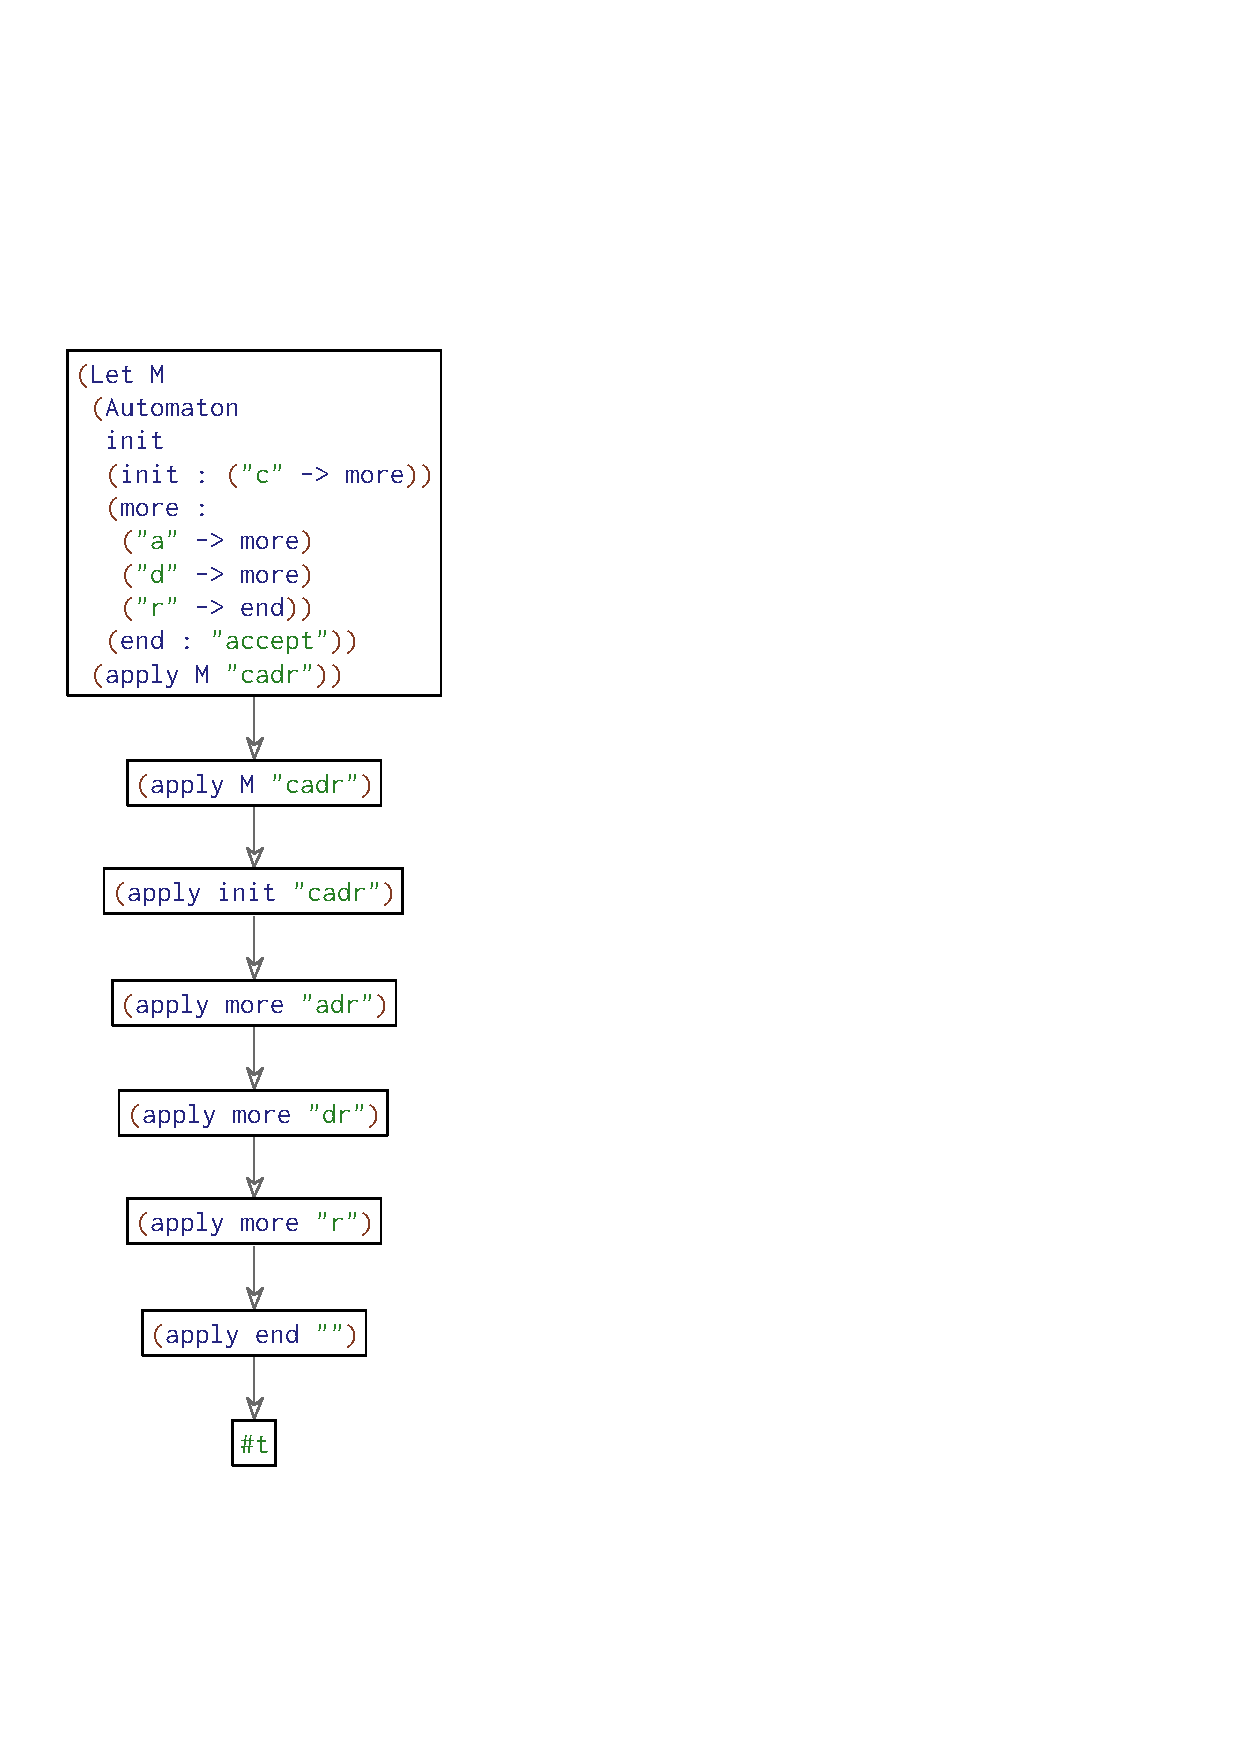
\includegraphics[width=0.45\columnwidth]{img/automaton-example}\hfill\mbox{}
\caption{Automaton macro execution example}
\label{fig:reval-automaton}
\end{figure}


\subsection{Return}
  Having first-class access to the current continuation is a powerful
  mechanism for defining new control flow constructs. Racket does so with
  the built-in function \Code{call/cc}, that takes a function of one
  argument and calls it with the program's current continuation. Using it,
  we can define a \Code{return} sugar that returns early from a function:
  \begin{Codes}
  Return(x) ->
    Let([Bind("\%RES", x)],
        [Apply(Id("\%RET"), [Id("\%RES")])]);

  Function(args, body) ->
    Lambda(args, Apply(Id("call/cc"),
                       [Lambda(["\%RET"], body)]));
  \end{Codes}
  (The definition of \Code{function} is necessary to mark the point that
  \Code{return} should return to.) With this definition in place, we can
  see evaluation sequences such as:
  \begin{Codes}
    (+ 1 ((function (x) (+ 1 (return (+ x 2)))) (+ 3 4)))
\SurfStep (+ 1 ((function (x) (+ 1 (return (+ x 2)))) 7))
\SurfStep (+ 1 (+ 1 (return (+ 7 2))))
\SurfStep (+ 1 (+ 1 (return 9)))
\SurfStep (+ 1 9)
\SurfStep 10
  \end{Codes}
  This example illustrates that our approach is robust enough to work even
  in the presence of dynamic control flow.


\subsection{Pyret: A Case Study}
\label{sec:reval-pyret}

Pyret, shown in \cref{sec:reval-pyret-example}, is a new language. It makes
heavy use of syntactic sugar to emulate the syntax of other programming
languages like Python. This sugar was implemented by people other than
this paper's authors, and written as a manual compiler, not as a set
of rules; it was also implemented without any attention paid to the
limitations of this work. Thus, the language makes for a good case
study for the expressiveness of our work.

We restricted our attention to sugar relevant to evaluation. Pyret has
builtin syntactic forms for writing tests, and can run code both in a
``check'' mode that only runs these tests, or in ``normal'' mode that runs
code. We focused on ``normal'' mode since it is most
relevant to evaluation. There were two pieces of sugar we
were unable to express and one that
required modification to show ideal surface steps; we
describe these in more detail below. 
As \cref{fig:reval-pyretsugar} shows, we were able to handle almost all
of Pyret's sugar. An example of the result in action was shown in
\cref{sec:reval-pyret-example}.

\begin{figure}
\begin{center}\small
\begin{tabular}{l | l c}
  \emph{\Sc{ast} Node} & \emph{Description} & \emph{Implemented?} \\ \hline
  fun & function declaration & yes \\
  when & one-arm conditional & yes \\
  if & multi-arm conditional & yes \\
  cases & multi-arm conditional & yes \\
  cases-else & multi-arm conditional & yes \\
  for & generalized looping construct & yes \\
  op & binary operators & yes \\
  not & negation & yes \\
  paren & grouping construct & yes \\
  left-app & infix notation & yes \\
  list & list expressions & yes \\
  dot & indirect field lookup & yes \\
  colon & direct field lookup & yes \\
  (currying syntax) & allowed in \Code{fun} and \Code{op} & yes \\
\hline
  graph & create cyclic data & no \\
  datatype & datatype declarations & no
\end{tabular}
\end{center}
\caption{Syntactic sugar in normal-mode Pyret}
\label{fig:reval-pyretsugar}
\end{figure}

We were unable to fully handle algebraic datatype declarations
because they splice one block of code into another in a non-compositional
manner; we believe these could be expressed by adding a block
construct that does not introduce a new scope (akin to Scheme's
\Code{begin}).

We were also unable to handle \Code{graph}, which constructs cyclic data.
It has a
complex desugaring that involves creating and updating placeholder values
and compile-time substitution. This could be solved either by expanding
the expressiveness of our system or by adding a new core construct to the
language. There is always a trade-off between the complexity of the core
language and the complexity of the desugaring; when a feature can only be
implemented through a highly non-compositional sugar like this, it may
make sense to instead add the feature to the core language.

Finally, the desugaring for binary operators needed to be modified to show helpful
surface evaluation sequences. The desugaring follows
a strategy similar to that of Python, by applying the \Code{\_plus} method
of the left subexpression to the right subexpression (the \Code{s} terms
are source locations, used for error-reporting):
\begin{Codes}
  Op(s, "+", x, y)  ->
    App(s, Bracket(s, x, Str(s, "_plus")), [y]);
\end{Codes}
Given the term \Code{1 + (2 + 3)}, we would expect evaluation to step
first to \Code{1 + 5} and then to \Code{6}. Unfortunately, {\Resugarer}
shows only this surface evaluation sequence:
\begin{Codes}
    1 + (2 + 3) \SurfStep 6
\end{Codes}
The core evaluation sequence reveals why:
\begin{Codes}
    1.["_plus"](2.["_plus"](3))
\CoreStep <func>(2.["_plus"](3))
\CoreStep <func>(<func>(3))
\CoreStep <func>(5)
\CoreStep 6
\end{Codes}
(\Code{<func>} denotes a resolved functional). To show the
term \Code{1 + 5}, Emulation requires that it desugar
precisely into one of the terms in the core sequence; but it desugars
to \Code{1.["\_plus"](5)}, which has a different shape than any of the
core terms.

The fundamental problem is the order of evaluation induced by this
desugaring: first the left subexpression is evaluated, then the
\Code{\_plus} field is resolved, then the right subexpression is
evaluated, then the ``addition'' is performed. We can obtain a more
helpful surface sequence by instead choosing a desugaring
that forces the left and right subexpressions to be evaluated fully before
resolving the operation, as shown in \cref{fig:reval-alt-plus}.

\begin{figure}[t]
\begin{Codes}
  Op(s, "+", x, y) ->
    Block(s,
    [ Let(s, Bind(s, "temp", ABlank),
             Obj(s, [Field(s, Str(s, "left"), x),
                     Field(s, Str(s, "right"), y)]))
    , App(s, Bracket(s, Bracket(s, Id(s, "temp"),
                                   Str(s, "left")),
                        Str(s, "_plus")),
             [Bracket(s, Id(s, "temp"),
                         Str(s, "right"))])]);
\end{Codes}
\caption{Alternate desugaring of addition}
\label{fig:reval-alt-plus}
\end{figure}
This desugaring constructs a temporary object \Code{\{left: x, right:
  y\}}, and then computes \Code{temp.left.\_plus(temp.right)}. Notice that
this desugaring \emph{slightly} changes the semantics of binary operators;
the difference may be seen when the right subexpression mutates the
\Code{\_plus} field of the left subexpression. In exchange, we obtain the
expected surface evaluation sequence:
\begin{Codes}
    1 + (2 + 3) \SurfStep 1 + 5 \SurfStep 6
\end{Codes}


\section{Obtaining Hygiene}
\label{sec:reval-hygiene}

The implementation discussed in this chapter---{\Resugarer}---is not
hygienic. (For a quick introduction to hygiene, see
\cref{sec:taxonomy-safety}.) In this section, we sketch out how {\Resugarer}
could be modified to be hygienic. More specifically, we show how it
can be modified such that variables defined by users are never bound
by variables defined by sugars, and vice-versa.\marginpar{The version
  of hygiene we are discussing here is the typical
  definition~\cite{hygienic-macros}.  In the next chapter, we will
  give a stronger definition.}

The required modification is simple. Suppose that:
\begin{itemize}[noitemsep]
  \item $\ExpandRecf$ gives fresh names to introduced variables (that
    is, variables on the \Sc{rhs}).
  \item $\UnexpandRecf$ allows any variable name to match against an
    introduced variable.
\end{itemize}
Then both $\ExpandRecf$ and $\UnexpandRecf$ will be hygienic:
user-defined variables and sugar-introduced variables will never be
bound by one another.

During \emph{desugaring}, sugar-introduced variables are those that
appeared as variables in the \Sc{rhs} of a sugar. By assumption, all
of these variables are given fresh names; thus no user-defined
variable can be bound by them, and vice-versa. Why is this proof so
easy, when significant effort has gone into defining hygienic macro
expansion algorithms? It is because we are assuming that sugars are
defined externally to the language, so they aren't intermingled with
user-defined code.

During \emph{resugaring}, it may look like there are no
sugar-introduced variables, since the \Sc{lhs}s of desugaring rules
cannot contain variables. However, the \Sc{lhs} of a rule \emph{can}
contain a pattern variable with a variable in it, and that pattern
variable \emph{can} be dropped on the \Sc{rhs}. In this case,
resugaring will restore that pattern variable, thereby re-introducing
its variables. For example, if \Code{(Lambda x.\ x * 0)} desugars into
\Code{(Lambda x.\ 0)}, then the \Code{x} in \Code{x * 0} will be
re-introduced by resugaring.

Is this re-introduced variable bound by the outer \Code{x}?
Surprisingly, it is not. The key point is that \emph{in the absense of
  surface-language scoping rules, where a variable is bound in a
  surface term is defined by the desugaring of that term.}
Since the inner \Code{x} is dropped during desugaring, it has no
binding site. Thus unexpansion is hygienic: every variable that is
re-introduced during resugaring has no binding site, so there can be
no accidental variable capture. The textual representation of the
surface term is misleading in this case. If {\Resugarer} made the
binding structure of the surface term explicit by, e.g., drawing
arrows to show where variables were bound, then it would be visibly
clear that the inner \Code{x} was not bound by the outer \Code{x}.

This may seem like a cop-out, but it is the best that we can do when
the scope of the surface language is defined only implicitly through
desugaring. In the next chapter, we will show how to \emph{resugar
  core language scope rules} to obtain scope rules for the surface
language, which will lead to a stronger notion of hygiene.

% NOTE (from the perspective of the next chapter):
% If you allow a desugaring rule to delete a pattern variable,
% then resugaring will not technically be hygienic. For example,
% suppose that (lambda x. x) => (lambda x. 3). This is a legit
% desugaring, but during resugaring 'x' will be captured! So I think
% this hygiene violation is OK. HOWEVER, we don't seem to need/want to
% drop pattern variables ANYWAYS, so I'm just stating the stronger
% property.

\section{Related Work}

There is a long history of trying relate compiled code back to its
source. This problem is especially pronounced in debuggers for
optimizing compilers, where the structure of the source can be altered
significantly~\cite{hennessy-debugging}. Most of this literature
is based on black-box
transformations, unlike ours, which we assume we have full control
over.  As a result, this work tends to be very different in flavor
from ours: some of it is focused on providing high-level
representations of data on the heap, which is a strict subproblem of
ours, or of correlating back to source expression \emph{locations}, which
again is weaker than \emph{reconstructing a source term}.
For this reason,
this work is usually also not accompanied by strong semantic
guarantees or proofs of them.

One line of work in this direction is SELF's debugging
system~\cite{self-debugging}. Its compiler provides its debugger with
debugging information at selected breakpoints by (in part) limiting the
optimizations that are performed around them. This is a sensible approach
when the code transformation in question is optimization and can be turned
off, but does not make sense when the transformation is a desugaring
which is necessary to give the program meaning.

Another line of work in this direction is the compile-time macro error
reporting developed by Culpepper, et al.~\cite{fortifying-macros}.
Constructing useful error messages is a difficult task that we have not
yet addressed. It has a different flavor than the problem we address,
though: akin to previous work in debugging, any source terms mentioned in
an error appear directly in the source, rather than having to be
reconstructed.

Deursen, et al.~\cite{deursen:origin-tracking} formalize the concept of
tracking the origins
of terms within term rewriting systems (which in their case represent
the \emph{evaluator}, not the \emph{syntactic sugar} as in our
case). They go on to show various applications, including
visualizing program execution, implementing debugger breakpoints,
and locating the sources of errors.
Their work does not involve the use of syntactic sugar,
however, while our work hinges on the interplay between syntactic
sugar and evaluation. Nevertheless, we
have adopted their notion of origin tracking for our transformations.

Krishnamurthi, et al.~\cite{sk:mcmicmac} develop a macro system meant
to support a variety of tools, such as type-checkers and
debuggers. Tools can provide feedback to users in terms of the
programmer's source using source locations recorded during
transformation. The system does not, however, reconstruct source
terms; it merely point out relevant parts of the original source.  The
source tracking mechanisms are based on Dybvig, et al.'s macro
system~\cite{expansion-passing-style}.

Clements~\cite[page 53]{clements:thesis} implements an algebraic
stepper (similar to ours) for Racket---a language that has
macros---and thus faces precisely the same problem we address in this
paper. That work, however, side-steps these issues by handling a
certain fixed set of macros specially (those in the ``Beginner
Student'' language) and otherwise showing only expanded code.
On the other hand, it proves that its method of instrumenting a program to
show evaluation steps is correct (i.e., the instrumented program shows the
same evaluation steps that the original program produces),
while we only show that the lifted evaluation sequence is correct
with respect to the core stepper. Thus its approach could be
usefully composed with ours to achieve stronger guarantees.

Fisher and Shivers~\cite{ziggurat} develop a framework
for defining static semantics that connect the
surface and core languages. They show how to effectively \emph{lower}
a \emph{static} semantics from a surface language to its core
language. This is complementary to our work, which
shows how to \emph{lift} a \emph{dynamic} semantics from core to surface.
This exposes a fundamental difference in starting assumptions:
they assume the surface language has a static semantics, while we assume
its semantics is \emph{defined} by desugaring.

In a similiar vein, Lorenzen and Erdweg \cite{typechecking-exts} give a
method for ensuring the type soundness of syntactic extensions by lowering
author-provided typing rules for the surface language onto the core
language's type system (and automatically verifying that soundness is
entailed). Thus their work does for type checking what ours does for
evaluation: it provides a surface type checker guaranteed to be sound with
respect to the core language, while ours produces a surface evaluator
guaranteed to emulate the core language.

Model-driven software engineering also draws heavily on
bidirectional transformation, because systems are expected to be written
in a collection of domain-specific languages that are transformed into
implementations. These uses tend to be \emph{static}, rather
than addressing the inverse-mapping problem in the context of system
execution (see the survey by
Stevens~\cite{bidirectional-model-transfs}).
When the problem we address does arise in this area, it is typically the
case that either (i) both the source and target models have
implementations, so that surface-level execution traces can be obtained
by evaluating in the surface language directly~\cite{Perera-slicing}, or
(ii) the surface information sought is more limited than the reduction
sequence we provide (in the same ways as for debuggers for optimizing
compilers, as described earlier).
Applying our results to this area is future work.

\chapter{Resugaring Scope}\label{chap:resugar-scope}

In this chapter, we show how to lift scoping rules defined on a core
language to rules on the surface, a process of \emph{scope inference}.
In the process we introduce a new representation of binding
structure---scope as a preorder---and present a theoretical advance:
proving that a desugaring system preserves $\alpha$-equivalence even
though scoping rules have been provided \emph{only} for the core
language.

This chapter comes from work published in ICFP 2017 under the title
\emph{Inferring Scope through Syntactic Sugar} (co-authored with
Shriram Krishnamurthi and Mitchell Wand)~\cite{pombrio-scope}.

\section{Introduction}

Traditionally,
scoping rules are defined on the core language, not on the
surface. However, many tools depend on source representations. For
instance, editors need to know the surface language's scoping in order
to perform auto-complete, distinguish free from bound variables, or draw
arrows to show bound and binding instances. Likewise, refactorers need
to know binding structure to perform correct transformations.
These tools are hard to construct if scoping is only known
for the core language.

Many tools that exploit binding information for the source
do so by desugaring the program and obtaining its binding in the core
language (this, for instance, is the approach used by
DrRacket~\cite{drscheme} for overlaying binding arrows on the
source).
However, this approach is far from ideal. It requires tools to be able
to desugar programs and to resolve binding in the core
language. This is an intimate level of knowledge of a language, though:
syntactic sugar is supposed to be an abstraction, so external tools
should ideally be unaware that a language even \emph{has} syntactic
sugar. Additionally, this approach fails completely if the source
program cannot be desugared because it is incomplete or syntactically
invalid (as programs are most of the time while editing). It is
therefore better to disentangle the editor from the language,
providing the editor precisely what it needs: scoping rules for the
surface language.

We therefore present a static inference process that, given a
specification of syntactic sugar and scoping rules on a core language,
\emph{automatically constructs} scoping rules for the surface
language. The inferred rules are guaranteed to give the same binding
structure to a surface program as that program would have in the core language
after desugaring (\cref{thm:rscope-resugar}).
Essentially, scope inference ``pushes scope back through the sugar''. We
can think of this as statically lifting a ``lightweight semantics'' of
the language. Thus it is a precursor to lifting other notions of semantics
(such as lifting type-checking rules, as we do in the next chapter)
though of course the mechanics of doing so will depend heavily on the
semantics itself.

The intended application of this work is as follows:
\begin{enumerate}
\item Begin with a core language with known scoping rules, and a set
  of pattern-based desugaring rules. (We give a formal description of
  scope in \cref{sec:rscope-sap}, and a language for specifying scope in
  \cref{sec:rscope-rules}.)
\item Infer surface language scoping rules from the core scoping
  rules. (We give a scope inference algorithm in
  \cref{sec:rscope-resugar}, and show how to make it hygienic in
  \cref{sec:rscope-hygiene}.)
\item Add these inferred scoping rules to various tools that can exploit
  them (Sublime, Atom, CodeMirror, etc.).
\end{enumerate}

An alternative approach would be to specify scoping rules for the
surface language, and verify that they are consistent with the core
language. This approach has been advocated for
scoping~\cite{herman-hygiene,stansifer-romeo},
type systems~\cite{typechecking-exts},
and formal semantics~\cite{ziggurat}.
However, this assumes that language developers are always programming
language experts who are knowledgeable about binding, able to verify consistency, and willing
to do this extra work. These are particularly unsafe assumptions for
domain-specific languages, which we believe are a strong use case for
our technique.

\subsection*{Contributions and Outline}
\begin{description}
\item[Modelling Scope] In \cref{sec:rscope-sap}, we give a formal
  description of scope as a \emph{preorder} 
  (which we motivate through examples in
  \cref{sec:rscope-example}).
  This preorder then defines the name
  binding structure of a program, such as where variable
  references are bound, and which variable declarations shadow others.
\item[Binding Specification Language] In \cref{sec:rscope-rules}, we
  present a \emph{binding specification language}, i.e., a language
  for specifying the name binding structure of a programming
    language. This specification makes it possible to compute the
    scope structure (a preorder) of concrete programs in that language.
  \item[Scope Inference] In \cref{sec:rscope-resugar}, we show how to
  \emph{infer} these scoping rules through syntactic sugar. This is our main contribution. We describe our
  implementation and provide case studies in
  \cref{sec:rscope-impl}, and prove that---given reasonable
  assumptions---desugaring after scope inference will be hygienic in
  \cref{sec:rscope-hygiene}.
\end{description}


\section{Two Worked Examples}\label{sec:rscope-example}

We will begin by building up to our scope inference technique via two
worked examples.
\textbf{They are slightly simplified for expository purposes}. 
\Cref{sec:rscope-rules} describes the generalization, and
\cref{sec:rscope-for-example,sec:rscope-named-let-example}
provide examples.
(While the generalization is sometimes important, it has no effect on the
examples of this section.)

\subsection{Example: Single-arm Let}
For the first example, consider a simple Let construct that allows
only a single binding:
\begin{Table}
  $e$ &$::=$& $\NodeRm{Let}{\DeclX\;e_1\;e_2}$
  & ``Let $\DeclX$ equal $e_1$ in $e_2$'' \\
  &$|$& $\ldots$
\end{Table}
(Here the superscript \textsc{d} indicates that this
occurrence of the variable $\VarX$ is a declaration of $\VarX$.
In general, we
will distinguish \emph{declarations}, i.e., binding sites, from
\emph{references}, i.e., use sites.)

This Let may be desugared to Apply and Lambda by the following desugaring rule, which
we will write using s-expressions:
\begin{LongTable}
  $\NodeRm{Let}{\PVarA\;\PVarB\;\PVarC}$
  &$\To$&
  $\NodeRm{Apply}{\NodeRm{Lambda}{\PVarA\;\PVarC}\;\PVarB}$
\end{LongTable}

Now suppose that we know the scoping rules of Apply and Lambda, and
wish to derive what the scoping rules for Let must be, given
the desugaring rule and assuming the language is statically and lexically
scoped. More precisely, we wish to find a scoping rule
for Let such that the desugaring rules \emph{preserve binding structure}
(and thus neither cause variable capture nor cause
variables to become unbound).

The first step will be to write down what we know about the
scope on the \textsc{rhs} (right hand side) of the rule.
Pictorially, we might draw:
\begin{center}
\sideLabel{\textsc{rhs}}{
\begin{tikzScopeDiagram}[simple]
  \tikzRoot
    {A}{\tikzParentTwo{Apply}
      {B}{\tikzParentTwo{Lambda}
        {C}{\tikzChild{$\PVarA$}}
        {D}{\tikzChild{$\PVarC$}}}
      {G}{\tikzChild{$\PVarB$}}}
  \begin{tikzEdges}
    \tikzEdgeL{C}{D};
  \end{tikzEdges}
\end{tikzScopeDiagram}
}
\end{center}
where the dotted lines show the tree structure of the \textsc{ast}, and
where the teal/solid arrow means that the Lambda's parameter ($\PVarA$) can be
used in its body ($\PVarC$).
Similarly, there are no arrows among the children
of Apply because function application does not introduce any binding.

We also know from lexical scope that any declarations in scope at a
node in an \textsc{ast} should also be in scope at its children. This
can be denoted with upward arrows:
\begin{center}
\sideLabel{\textsc{rhs}}{
\begin{tikzScopeDiagram}[simple]
  \tikzRoot
    {A}{\tikzParentTwo{Apply}
      {B}{\tikzParentTwo{Lambda}
        {C}{\tikzChild{$\PVarA$}}
        {D}{\tikzChild{$\PVarC$}}}
      {E}{\tikzChild{$\PVarB$}}}
  \begin{tikzEdges}
    \tikzEdgeL{C}{D};
    \tikzEdge{A}{B};
    \tikzEdge{A}{E};
    \tikzEdge{B}{C};
    \tikzEdge{B}{D};
  \end{tikzEdges}
\end{tikzScopeDiagram}
}
\end{center}
In general, the meaning of the arrows is that a variable declaration
is in scope at every part of the program which has a (directed) path to it.
(In the case of variable shadowing, the outer declaration is in scope
at the inner declaration, which in turn is in scope at some region;
references in this region will be bound to the dominating inner declaration.)

Now we can begin to infer what the scope must look like on the
\textsc{lhs} (left hand side) of the desugaring rule. We want the rule to
\emph{preserve} binding, therefore there should be a path from one
pattern variable to another in the \textsc{lhs} iff there is a similar path in the
\textsc{rhs}. If there was a path from $\PVarA$ to $\PVarB$ in the
\textsc{lhs} but not in the \textsc{rhs}, that would mean that a
variable (in $\PVarA$) that used to be bound (by $\PVarB$) could
become unbound. Likewise, if there was a path between two pattern variables in the
\textsc{rhs} but not in the \textsc{lhs}, that could result in
unwanted variable capture.

Thus, since there is a path from $\PVarC$ to $\PVarA$ in the rule's
\textsc{rhs}, there must also be a path from $\PVarC$ to $\PVarA$ in the
\textsc{lhs}. This gives:
\begin{center}
  \sideLabel{\textsc{lhs}}{
  \begin{tikzScopeDiagram}[simple]
    \tikzRoot
      {A}{\tikzParentThree{Let}
        {B}{\tikzChild{$\PVarA$}}
        {C}{\tikzChild{$\PVarB$}}
        {D}{\tikzChild{$\PVarC$}}}
    \begin{tikzEdges}
      \tikzEdgeL{B}{D};
    \end{tikzEdges}
  \end{tikzScopeDiagram}
  }
\end{center}
In English, this arrow says that the variable declared at $\PVarA$ is
in scope at the Let's body $\PVarC$, as expected.

There are still some missing arrows, however: there should be down
arrows to indicate that any declaration in scope at the Let should
also be in scope at its children. These can be inferred in a similar
way: whenever there is a path from the root to a pattern variable on the
\textsc{rhs}, there should be a similar path on the \textsc{lhs}.
Since on the \textsc{rhs} there are paths to each pattern variable from the root,
the same should hold true on the \textsc{lhs}:
\begin{center}
\sideLabel{\textsc{lhs}}{
\begin{tikzScopeDiagram}[simple]
  \tikzRoot
    {A}{\tikzParentThree{Let}
      {B}{\tikzChild{$\PVarA$}}
      {C}{\tikzChild{$\PVarB$}}
      {D}{\tikzChild{$\PVarC$}}}
  \begin{tikzEdges}
    \tikzEdgeL{B}{D};
    \tikzEdge{A}{B};
    \tikzEdge{A}{C};
    \tikzEdge{A}{D};
  \end{tikzEdges}
\end{tikzScopeDiagram}
}
\end{center}
This gives a complete scoping rule for this Let construct.


\subsection{Example: Multi-arm Let*}
\label{sec:rscope-example2}

Next, take a more involved example: a multi-armed Let* construct (in
the style of Lisp/Scheme/Racket).
It will have the following grammar:
\begin{Table}
  $e$ &$::=$& $\NodeRm{Let*}{b\;e}$
  & ``Let-bind $b$ in $e$'' \\
  &$|$& $\ldots$ \\
  $b$ &$::=$& $\NodeRm{Bind}{\DeclX\;e\;b}$
  & ``Bind $\DeclX$ to $e$, and bind $b$'' \\
  &$|$&   $\ConstRm{EndBinds}$
  & ``No more bindings''
\end{Table}
This grammar separates out the Let's bindings into nested
subterms.\marginpar{%
We call the bindings just ``Bind'', even though they are specific
  to Let. If a language has other forms of binding as well, ``Bind'' may need a more
  specific name such as ``LetBind''.
}
It is
necessary to do this if more complex binding patterns are allowed,
such as arbitrarily deep pattern-matching.

Let* can then be implemented with two desugaring rules:
\begin{LongTable}
$\NodeRm{Let*}{\NodeRm{Bind}{\PVarA\;\PVarB\;\PVarC}\;\PVarD}$
$\To$
$\NodeRm{Apply}{\NodeRm{Lambda}{\PVarA\;\NodeRm{Let*}{\PVarC\;\PVarD}}\;\PVarB}$
\\ \\
$\NodeRm{Let*}{\ConstRm{EndBinds}\;\PVarA}$
$\To$
$\NodeRm{Begin}{\PVarA}$
\end{LongTable}
These rules would, for example, make the following transformation:
\begin{Table}
$\NodeRm{Let*}{\NodeRm{Bind}{\DeclX\;1\;\NodeRm{Bind}{\DeclY\;2\;\ConstRm{EndBinds}}}\;\NodeRm{Plus}{\RefnX\;\RefnY}}$ \\
\quad $\To$
$\NodeRm{Apply}{\NodeRm{Lambda}{\DeclX\;\NodeRm{Apply}{\NodeRm{Lambda}{\DeclY\;\NodeRm{Plus}{\RefnX\;\RefnY}}\;2}}\;1}$
\end{Table}

Given that we know the scoping rules of Apply, Lambda, and Begin,
we can use them to derive the scoping rules for Let* and Bind. The scoping for
the second rule is trivial, so we will concentrate just on the first rule.

As before, the first step is to write down what we know about the
scope on the \textsc{rhs}:
\begin{center}
\sideLabel{\textsc{rhs}}{
\begin{tikzScopeDiagram}[simple]
  \tikzRoot
    {A}{\tikzParentTwo{Apply}
      {B}{\tikzParentTwo{Lambda}
        {C}{\tikzChild{$\PVarA$}}
        {D}{\tikzParentTwo{Let*}
          {E}{\tikzChild{$\PVarC$}}
          {F}{\tikzChild{$\PVarD$}}}}
      {G}{\tikzChild{$\PVarB$}}}
  \begin{tikzEdges}
    \tikzEdgeL{C}{D};
    \tikzEdge{A}{B};
    \tikzEdge{A}{G};
    \tikzEdge{B}{C};
    \tikzEdge{B}{D};
    \tikzEdge{D}{E};
    \tikzEdge{D}{F};
  \end{tikzEdges}
\end{tikzScopeDiagram}
}
\end{center}
Unlike in the previous example, this diagram is not (necessarily)
complete, since we don't yet know the scoping rule for
Let*. (This will happen when desugaring rules use recursion.)
We have drawn two upward arrows on Let*, despite the fact that we
don't yet know its scoping rule: technically, these arrows should
(and can) be inferred, but we start with them to simplify this example.

Now we can begin to infer what the scope must look like on the
\textsc{lhs}. As before, we want the rule to preserve
binding. Thus, since the \textsc{rhs} has a path from $\PVarC$ to
$\PVarA$ and from $\PVarD$ to $\PVarA$, the same must be true in the
\textsc{lhs} (labeling the arrows for reference):
\begin{center}
\sideLabel{\textsc{lhs}}{
\begin{tikzScopeDiagram}[simple]
  \tikzRoot
    {A}{\tikzParentTwo{Let*}
      {B}{\tikzParentThree{Bind}
        {C}{\tikzChild{$\PVarA$}}
        {D}{\tikzChild{$\PVarB$}}
        {E}{\tikzChild{$\PVarC$}}}
      {F}{\tikzChild{$\PVarD$}}}
  \begin{tikzEdges}
    \tikzEdgeRR{C}{E}[][c];
    \tikzEdge{C}{B}[][b];
    \tikzEdgeL{B}{F}[][a];
  \end{tikzEdges}
\end{tikzScopeDiagram}
}
\end{center}
Notice that we drew the path from $\PVarD$ to $\PVarA$ with \emph{two}
arrows. This is because we will assume that scoping rules are local,
relating only terms and their immediate children.

We have now learned something about the scoping rules for Let* and
Bind! When read in English, these three arrows say that:
\begin{enumerate}
\item[a.] Declarations from a Let*'s binding list are visible in its body.
\item[b.] A Bind's variable declaration is provided by the Bind (so
  that it can be used by the Let*).
\item[c.] A Bind's variable declaration is visible to later Binds in the
  binding list.
\end{enumerate}

This information can now be applied to fill in the previously
incomplete \textsc{rhs} picture. Arrow (a) represents a
fact about the scoping of \emph{every} Let*, so it must also apply in the
\textsc{rhs} (highlighting it orange/dashed for exposition):
\begin{center}
\sideLabel{\textsc{rhs}}{
\begin{tikzScopeDiagram}[simple]
  \tikzRoot
    {A}{\tikzParentTwo{Apply}
      {B}{\tikzParentTwo{Lambda}
        {C}{\tikzChild{$\PVarA$}}
        {D}{\tikzParentTwo{Let*}
          {E}{\tikzChild{$\PVarC$}}
          {F}{\tikzChild{$\PVarD$}}}}
      {G}{\tikzChild{$\PVarB$}}}
  \begin{tikzEdges}
    \tikzEdgeL{C}{D};
    \tikzEdge{A}{B};
    \tikzEdge{A}{G};
    \tikzEdge{B}{C};
    \tikzEdge{B}{D};
    \tikzEdge{D}{E};
    \tikzEdge{D}{F};
    \tikzEdgeL{E}{F}[color=arrowColorHL,dashed];
  \end{tikzEdges}
\end{tikzScopeDiagram}
}
\end{center}
Adding this arrow introduces a path from $\PVarD$ to $\PVarC$,
however, that needs to be reflected back at the \textsc{lhs}!
\begin{center}
\sideLabel{\textsc{lhs}}{
\begin{tikzScopeDiagram}[simple]
  \tikzRoot
    {A}{\tikzParentTwo{Let*}
      {B}{\tikzParentThree{Bind}
        {C}{\tikzChild{$\PVarA$}}
        {D}{\tikzChild{$\PVarB$}}
        {E}{\tikzChild{$\PVarC$}}}
      {F}{\tikzChild{$\PVarD$}}}
  \begin{tikzEdges}
    \tikzEdgeRR{C}{E}[][c];
    \tikzEdge{C}{B}[][b];
    \tikzEdgeL{B}{F}[][a];
    \tikzEdge{E}{B}[color=arrowColorHL,dashed][d];
  \end{tikzEdges}
\end{tikzScopeDiagram}
}
\end{center}
In general, the algorithm is to monotonically add arrows until
reaching the least fixpoint. In this particular case, arrow $d$ is the last
fact to be inferred:
\begin{enumerate}
\item[d.] A Bind also provides any declarations provided by later Binds
  in the binding list.
\end{enumerate}
This concludes the interesting facts to be inferred about the scoping
rules for Let* and Bind. We have ignored the upward arrows that reflect
lexical scope from parent to child for simplicity, but these can
be inferred by the same process.


\subsection{Scope as a Preorder}

In the two preceding examples, we have expressed the scope of a program
diagrammatically with arrows. When reasoning about scope, it will be
helpful to be able to \emph{transcribe} these diagrams into a
textual form.

To do so, recall the (approximate) meaning of the arrows:\marginpar{%
We make the meaning of arrows precise in \cref{sec:rscope-sap-defs}.
}
a declaration is in scope at every part of the program which has a
(directed) path to it, and is shadowed by declarations of the same name
that have a path to it. Thus the arrows are only meaningful insofar as
they produce paths. Furthermore, paths have two important properties:
\begin{enumerate}
  \item They are closed under reflexivity: there is always an (empty) path
    from $a$ to $a$.
  \item They are closed under transitivity: if there is a path from
    $a$ to $b$ and a path from $b$ to $c$, then there is a path from
    $a$ to $c$.
\end{enumerate}
These are also precisely the properties that define a \emph{preorder}.
Thus, we will transcribe scope diagrams as preorders, writing $a \< b$
when there is a path from $a$ to $b$.
For example, in the (incomplete) diagram we inferred for the \textsc{lhs} of the
multi-arm Let* sugar:
\begin{center}
\begin{tikzScopeDiagram}[simple]
  \tikzRoot
    {A}{\tikzParentTwo{Let*}
      {B}{\tikzParentThree{Bind}
        {C}{\tikzChild{$\PVarA$}}
        {D}{\tikzChild{$\PVarB$}}
        {E}{\tikzChild{$\PVarC$}}}
      {F}{\tikzChild{$\PVarD$}}}
  \begin{tikzEdges}
    \tikzEdgeRR{C}{E};
    \tikzEdge{C}{B};
    \tikzEdgeL{B}{F};
    \tikzEdge{E}{B};
  \end{tikzEdges}
\end{tikzScopeDiagram}
\end{center}
The corresponding preorder is:
$\hspace{2em} \PVarD \< \ConstRm{Bind} \< \PVarC \< \PVarA$



\section{Describing Scope as a Preorder}
\label{sec:rscope-sap}

We have informally described the notion of scope as a preorder,
primarily using diagrams. In this section, we will describe it
formally. First, however, we need to lay down some
starting assumptions and basic definitions.

\subsection{Basic Assumptions}
\label{sec:rscope-prelim}

We will make a number of assumptions to make reasoning about scope
more tractable:
  \begin{itemize}
  \item We only deal with scoping that is \emph{static} and \emph{lexical}.
  \item Scoping rules will be as local as possible, only relating a
    term to its \emph{immediate} children. Longer relationships will
    be achieved by transitivity.\marginpar{%
      If we allowed non-local arrows, then in the previous example,
      inference would produce a single arrow from $\PVarD$
      to $\PVarA$ instead of arrows ``a'' and ``b''. Then the orange/dashed arrow
      could \emph{not} be inferred, since it relied on the existence
      of arrow ``a'', and the inference process would fail at its task.
      }
  \item We work on an \textsc{ast}, instead of directly on the surface
    syntax. As mentioned in \cref{sec:formal-reqs},
    variable references (use sites) and declarations
    (binding sites) must be syntactically distinguished in this
    \textsc{ast}.
  \item Each kind of term has a fixed arity. (Indefinite arity is
    possible using a list encoding, as in Let* above.)
\end{itemize}

The last two of these assumptions are already reflected in our
definition of (\textsc{ast}) terms in \cref{sec:formal-term}.
For convenience, we repeat that definition here:

\begin{Table}
constructor $C$ &$::=$& \textit{name} & syntactic construct name \\
term $e$ &$::=$& $\Value$ & primitive value \\
  &$|$& $\Node{C}{e_1 \dd e_n}$ & \Sc{ast} node \\
  &$|$& $\Refn[i]{x}$  & variable reference at position $i$ \\
  &$|$& $\Decl[i]{x}$  & variable declaration at position $i$ \\
\end{Table}
To reiterate, references and declarations have both a name \textsc{x}
(as written in the source), and an \textsc{ast} position $i$
(that uniquely distinguishes them).
Occasionally it will be useful to refer to a variable which could be
either a declaration or a reference: in this case
we omit the superscript, e.g. $\VarXi$.
Likewise, we will omit the position subscript $i$
when there is no ambiguity. We will also sometimes write $C$ in place
of $\Node{C}{e_1\,...\,e_n}$ when there is no danger of ambiguity.

By the last assumption above, we do not support lists
$[e_1 \dd e_n]$ (which have indefinite arity). Instead we require them
to be encoded into fixed-arity constructs.

\subsection{Basic Definitions}
\label{sec:rscope-sap-defs}

  We define scope in terms of a perorder.
  A \emph{preorder} ($\<$) is a reflexive and transitive relation. It
  need not be anti-symmetric, however, so it is possible that $a \< b$
  and $b \< a$ for distinct $a$ and $b$.
We capture scope as a preorder on a term $e$ as follows:

\begin{definition}[Scope]\label{def:rscope-scope}
  A \emph{scope preorder} on a term $e$ is a preorder ($\<$) on the references
  and declarations in $e$ such that references are least in this
  preorder (i.e., nothing is ever smaller than a reference).
\end{definition}
\begin{definition}
  A reference $\RefnXi$ is \emph{in scope of} a declaration
  $\DeclXj$ when $\RefnXi \< \DeclXj$.
\end{definition}
\begin{definition}
  A declaration $\DeclXi$ is \emph{more specific than}
    another $\DeclXj$ when $\DeclXi \< \DeclXj$.
\end{definition}
Note that these definitions rely on the \emph{existence} of a preorder
($\<$), but don't say how to determine it for a given term. We will present
\emph{scoping rules} to do so in \cref{sec:rscope-rules}.
These definitions therefore provide very little on their own, but they can be built upon to define
some common concepts:

\begin{definition}[Bound]
  \label{def:rscope-bound}
  A reference is \emph{bound} by the most specific declaration(s) that
  it has the same name as and is in scope of. More formally, we write:
  \[ \RefnX \Bound \DeclX \Defeq
  \DeclX \in \min \St{\DeclXi}{\RefnX \< \DeclXi} \]
  where $\min S$ finds the (zero or more) least elements of $S$:
\[ \min S \Defeq \St{a \in S}{
  \NotExists{b \in S}
    b \< a \text{ and } a \not\< b}
\]
\end{definition}

\begin{definition}[Unbound]
A reference is \emph{unbound} (or \emph{free}) when it is not bound by
any declaration.
\end{definition}

\begin{definition}[Ambiguously Bound]\label{def:rscope-ambig}
  A variable reference is \emph{ambiguously bound} when it is bound by
  more than one declaration.
\end{definition}

Ambiguous binding may occur, for instance, if two declarations
have the same name and are both parameters to the same function.
In this case, a reference in the body of the function would be
ambiguously bound to both of them.
We also capture the idea of \emph{shadowing}, where a more specific
declaration hides a less specific declaration:

\begin{definition}[Shadowing]
  \label{def:rscope-shadow}
  \marginpar{%
We use the same notation $\square \Bound \square$ for both binding
and shadowing because the definitions are analogous.}
  A declaration \emph{shadows} the most specific declarations that it
  has the same name as and is more specific than. Formally, $\DeclXi$
  shadows $\DeclXj$ when:
  \[ \DeclXi \Bound \DeclXj \Defeq
  \DeclXj \in \min \St{\DeclXk}{i \neq k \text{ and } \DeclXi \< \DeclXk}
  \]
\end{definition}

\subsection{Validating the Definitions}
Since this description of scope is new, readers might wonder
whether our definitions of concepts match their vernacular meaning.
We provide evidence that they do in three forms.

First, we prove a simple lemma below showing that shadowing
behaves as one would expect.
Second, we show (\cref{sec:rscope-sos}) that the notion of scope used in
``Binding as Sets of Scopes''~\cite{flatt:scope} obeys our {\sap}
definitions, for an appropriate choice of preorder $(\<)$.
Finally, we introduce a second, very intuitive definition of
scope called {\sas}, and show that it is equivalent to {\sap} up to
a normalization.

\begin{lemma}[Shadowing]
  If one declaration shadows another, then a reference in scope of the
  shadowing declaration cannot be bound by the shadowed declaration.
\end{lemma}
\begin{proof}
  Suppose that $\DeclXj$ shadows $\DeclXi$ ($\DeclXj$ is the shadowing
  declaration and $\DeclXi$ is the shadowed declaration), and
  $\RefnXk$ is in scope of $\DeclXj$.
  By definition, $\RefnXk$ will be bound by
  $\min \St{\DeclXl}{\RefnXk \< \DeclXl}$.  But $\RefnXk \<
  \DeclXj \< \DeclXi$, so $\DeclXi$ cannot be in this set, and $\RefnXk$
  cannot be bound by $\DeclXi$.
\end{proof}

\subsection{Relationship to ``Binding as Sets of Scopes''}
\label{sec:rscope-sos}
{\Sap} aligns with the notion of scope expressed by Flatt~\cite{flatt:scope}.
In his formulation,
each subterm in the program is labeled with a \emph{set of scopes},
called its \emph{scope set}. A reference's binding (i.e., declaration)
is then found ``as one whose set of scopes is a subset of the
reference's own scopes (in addition to having the same symbolic
name)''. If there is more than one such declaration, a reference is
bound by the one with the largest (superset-wise) scope set. If there
is no unique such element, then the reference is
``ambiguous''~\cite[pp. 3]{flatt:scope}.

This can be expressed in terms of {\sap}. Take the preorder
$(\<)$ to be (the least relation such that):
\begin{Table}
$\RefnXi \< \RefnXi$ \\
$\RefnX \< \DeclY$   iff $\Scopeset{\RefnX} \supseteq \Scopeset{\DeclY}$ \\
$\DeclXi \< \DeclYj$ iff $\Scopeset{\DeclXi} \supseteq \Scopeset{\DeclYj}$
\end{Table}
Then our definition of a reference's binding agrees with Flatt's, and
our definition of an ``ambiguously bound'' reference agrees with his
definition of an ``ambiguous'' reference.

\subsection{Axiomatizing Scope as Sets}
\label{sec:rscope-sas}

In this section, we describe an alternative axiomatization of scope,
called \emph{\sas}.
In {\sas}, instead of there being a preorder over variables, each
declaration has a \emph{scope}, which is the part of the program in
which it can be referenced. For example, the scope of a function's
parameter is that function's body. The axioms for a term $e$ are then:

\begin{description}
\item[Scope]
  Each declaration in $e$ has a \emph{scope}---written
  $\Scope{\DeclX}$---given by the parts of the program in which it can
  be referenced.
  We will say that:
  \begin{itemize}
  \item A reference $\RefnX$ is \emph{in scope of} a declaration
    $\DeclX$ when $\RefnX \in \Scope{\DeclX}$.
  \item One declaration $\DeclX$ is \emph{more specific than} another
    $\DeclY$ when $\Scope{\DeclX} \subseteq \Scope{\DeclY}$.
  \end{itemize}
\item[Binding]
  A reference is \emph{bound} to the most specific declaration that
  it has the same name as and is in scope of, provided such a unique
  element exists. Again, if there is no (unique) most specific
  declaration, we will say that the reference is \emph{ambiguously
    bound}.
%% \item[Renamability]
%%   The scope of a declaration is determined solely by the shape
%%   of the term it is in (and, in particular, not by the name of any
%%  variable).
\end{description}

These axioms differ from the {\sap} definitions in that the relations
``in scope of'' and ``more specific than'' are defined differently.
However, all of the other definitions of \cref{sec:rscope-sap}
(including binding, shadowing, ambiguous declarations, etc.)
are based on the relations ``in scope of'' and
``more specific than''. Thus all of those definitions apply just as
well to {\sas}.

Furthermore, the two axiomatizations of scope we have presented are closely
related. In fact, {\sap} is simply a normalized form of {\sas}.
To begin with, either form can be converted to the other.

\paragraph{\textit{Conv1}: From {\sap} to {\sas}}
Given a preorder ($\<$), define its conversion into a {\sas}
function $\Scope{}$ by:
\[ \Scope{\DeclY} \Defeq
   \St{\RefnX}{\RefnX \< \DeclY}
   \cup
   \St{\DeclX}{\DeclX \< \DeclY} \]

\paragraph{\emph{Conv2}: From {\sas} to {\sap}}
Given a {\sas} function $\Scope{}$, define its conversion into a
preorder ($\<$) by letting ($\<$) be the least relation such that:
\begin{Table}
  $\RefnXi \< \RefnXi$ \\
  $\RefnX \< \DeclY$
  &when& $\RefnX \in \Scope{\DeclY}$ \\
  $\DeclX \< \DeclY$
  &when& $\Scope{\DeclX} \subseteq \Scope{\DeclY}$
\end{Table}

Both of these conversions preserve all of the binding concepts of
\cref{sec:rscope-sap-defs}:

\begin{lemma}[Binding Preservation] \label{thm:rscope-preservation}
  Both $\ConvA{}$ and $\ConvB{}$ preserve ``in scope of'' and ``more
  specific than'' in both directions
  (and thus all of the concepts of \cref{sec:rscope-rules}).
\end{lemma}
\begin{proof}
  Under both conversions, ``in scope of'' is preserved:
  \begin{Table}
    \hphantom{iff}\; $\RefnX$ in scope of $\DeclY$ (under {\SAS}) \\
    iff\; $\RefnX \in \Scope{\DeclY}$ \\
    iff\; $\RefnX \< \DeclY$ \\
    iff\; $\RefnX$ in scope of $\DeclY$ (under {\SAP})
  \end{Table}

  And under both conversions, ``more specific than'' is preserved:
  \begin{Table}
    \hphantom{iff}\;
          $\DeclX$ more specific than $\DeclY$ (under {\SAS}) \\
    iff\; $\Scope{\DeclX} \subseteq \Scope{\DeclY}$ \\
    iff\; $\DeclX \< \DeclY$ \\
    iff\; $\DeclX$ more specific than $\DeclY$ (under {\SAP})
  \end{Table}
\end{proof}

Furthermore, these conversions are inverses in one direction: from
{\sap} to {\sas} back to {\sap}. This implies that there is a normal
form for {\sas}, given by $\ConvA{\ConvB{\Scope{}}}$, such that the
conversions are exact inverses whenever this normal form is used.

We first show that the conversions are inverses in one direction:
\begin{lemma}[Inverses1] \label{lemma:rscope-inverses}
  For every scope preorder ($\<$),
  $\ConvB{\ConvA{\<}} = (\<)$
\end{lemma}
\begin{proof}
  \begin{Table}
    $\RefnXi \< \RefnXj$
    &when& $i = j$ \\
    $\RefnX \< \DeclY$
    &when& $\RefnX \in \Scope{\DeclY}$ \\
    && iff $\RefnX \in \St{\RefnX}{\RefnX \< \DeclY}$ \\
    && iff $\RefnX \< \DeclY$ \\
    $\DeclX \< \DeclY$
    &when& $\Scope{\DeclX} \subseteq \Scope{\DeclY}$ \\
    && iff $\DeclX \< \DeclY$
  \end{Table}
\end{proof}

And they're inverses in the other direction when $\Scope{}$ is in a
\emph{normal form}. Specifically, we will say that a
{\sas} function $\Scope{}$ is in \emph{normal form} when:
\begin{Table}
  &(i)&  $\Forall{\DeclX} \Scope{\DeclX}$ contains only variables \\
  &(ii)& $\Forall{\DeclX} \Forall{\DeclY}
    \DeclX \in \Scope{\DeclY}
    \text{ iff } \Scope{\DeclX} \subseteq \Scope{\DeclY}$
\end{Table}

\begin{lemma}[Inverses2]
  For any {\sas} function $\Scope{}$ in normal form,\\ %NEWLINE
  $\ConvA{\ConvB{\Scope{}}} = \Scope{}$.
\end{lemma}
\begin{proof}
  \begin{LongTable}
    && $\Scope{\DeclY}$ \\
    &$=$& $\St{\RefnX}{\RefnX \< \DeclY} \cup
           \St{\DeclX}{\DeclX \< \DeclY}$
           &($\ConvA{}$) \\
    &$=$& $\St{\RefnX}{\RefnX \in \Scope{\DeclY}} \cup$ \\
       && $\St{\DeclX}{\Scope{\DeclX} \subseteq \Scope{\DeclY}}$
           &($\ConvB{}$) \\
    &$=$& $\St{\RefnX}{\RefnX \in \Scope{\DeclY}} \cup
           \St{\DeclX}{\DeclX \in \Scope{\DeclY}}$
           &(by (ii)) \\
    &$=$& $\Scope{\DeclY}$ &(by (i))
  \end{LongTable}
\end{proof}

The normal form of a {\sas} scope function can be computed as:
\[ \Norm{\Scope{}} = \ConvA{\ConvB{\Scope{}}} \]

\begin{lemma}
  For any {\sas} scope function $\Scope{}$, $\Norm{\Scope{}}$ is in
  fact in normal form.
\end{lemma}
\begin{proof}
  The first requirement---that the range of $\Scope{}$ only contains
  variables---is immediately fulfilled by $\ConvA{}$. The second
  requirement follows from the definitions of $\ConvA{}$ and $\ConvB{}$: \\
  $\DeclX \in \Scope{\DeclY}$
  iff $\DeclX \< \DeclY$
  iff $\Scope{\DeclX} \subseteq \Scope{\DeclY}$
\end{proof}

Putting a {\sas} scope function in normal form preserves its binding
structure. Furthermore, once it is in normal form, converting it to
{\sap} (and back) have no effect.

\begin{lemma}
  $\Norm{}$ preserves ``in scope of'' and ``more specific than''
  (and thus all of the concepts of \cref{sec:rscope-rules}).
\end{lemma}
\begin{proof}
  Follows directly from \cref{thm:rscope-preservation}.
\end{proof}

This concludes the demonstration that {\sap} is simply a normalized
version of {\sas}, and can effectively be used in its place. The
axioms of {\sas} are basic enough that they ought to apply in
basically any lexically-scoped setting; thus {\sap} should too.
We use {\Sap} in this thesis, however, because it is more canonical (per
normalization) and because it more closely aligns with the binding
language described next.



\section{A Binding Specification Language}
\label{sec:rscope-rules}

The previous section presented definitions for \emph{representing} the
scoping of a term. It did not, however, say how to \emph{determine}
the scoping of a term, i.e., what the specific preorder should be. In
this section, we give a language for specifying \emph{scoping rules}
that, given a term, determine a preorder over its variables.

\subsection{Scoping Rules: Simplified}

The basic idea behind our binding language is that the binding structure of
a term should be determined piecewise by its subterms. Thus every term
constructor (e.g., Lambda or Bind) should specify a \emph{scoping rule}
that gives a preorder amongst itself and its children. A term's {\sap}
can then be found by taking the transitive closure of these local
preorders across the whole term.

As an example, take the term
$\NodeRm{Lambda}{\DeclX[1]\;\NodeRm{Plus}{\RefnX[2]\;3}}$.  To find
the bindings of this term, we must know the scoping rules for Lambda
and Plus. A sensible rule for Plus is that a term
$\NodeRm{Plus}{\PVarA\;\PVarB}$ has preorder
$\PVarA \< \NodeRm{Plus}{\PVarA\;\PVarB}$
and $\PVarB\< \NodeRm{Plus}{\PVarA\;\PVarB}$,
meaning that whatever a Plus term is in scope of, its
children are too.
For brevity, we will typically write $\PVarA \< \ConstRm{Plus}$
and $\PVarB\< \ConstRm{Plus}$ instead.
Likewise, a sensible rule for Lambda is that a term
$\NodeRm{Lambda}{\PVarA\;\PVarB}$ has preorder $(\PVarB \< \PVarA
\< \ConstRm{Lambda})$,
meaning that whatever a Lambda term is in scope of, its
children are too, and that $\PVarB$ (its body) is in
scope of $\PVarA$ (its declaration). Put together, and applied to the
example term, these rules give that:
\[  \NodeRm{Lambda}{\DeclX[1]\;\NodeRm{Plus}{\RefnX[2]\;3}} \]
has preorder:
\[
  \RefnX[2], 3 \<
  \ConstRm{Plus} \< \DeclX[1] \< \ConstRm{Lambda}
\]
Thus $\RefnX[2] \Bound \DeclX[1]$ by \cref{def:rscope-bound}, as it should be.


\subsection{A Problem}

This isn't quite the whole picture, though. Consider the term
\[
\NodeRm{Lambda}{\DeclX[1]\;
  \NodeRm{Let*}{
    \NodeRm{Bind}{\DeclX[2]\;\RefnX[3]\;\ConstRm{EndBinds}}\;
    \RefnX[4]}}
\]

What will these scoping rules look like? Whatever they are, they
should cause $\DeclX[2]$ to shadow $\DeclX[1]$, $\RefnX[3]$ to be
bound by $\DeclX[1]$, and $\RefnX[4]$ to be bound by $\DeclX[2]$.
Formally, we should have:
\[ \DeclX[2] \Bound \DeclX[1] \text{ and }
   \RefnX[3] \Bound \DeclX[1] \text{ and }
   \RefnX[4] \Bound \DeclX[2]
\]
which implies that, at a minimum:
\[ \DeclX[2] \< \DeclX[1] \text{ and }
   \RefnX[3] \< \DeclX[1] \text{ and }
   \RefnX[4] \< \DeclX[2]
\]

This places a set of requirements on the scoping rules for Lambda,
Let*, and Bind. For instance, $\RefnX[3] \< \DeclX[1]$ can only be
achieved if $\RefnX[3] \< \ConstRm{Bind} \< \ConstRm{Let*} \< \DeclX[1]$.
Continuing this way gives the requirements (shown both pictorially and
textually):

\begin{scopeDescription}
\begin{center}
\begin{tikzScopeDiagram}[simple]
  \tikzRoot
    {A}{\tikzParentTwo{Lambda}
      {B}{\tikzChild{$\DeclX[1]$}}
      {C}{\tikzParentTwo{Let*}
        {D}{\tikzParentThree{Bind}
          {E}{\tikzChild{$\DeclX[2]$}}
          {F}{\tikzChild{$\RefnX[3]$}}
          {G}{\tikzChild{EndBinds}}}
        {H}{\tikzChild{$\RefnX[4]$}}}}
      
  \begin{tikzEdges}
    \tikzEdgeL{B}{C};
    \tikzEdge{C}{D};
    \tikzEdgeL{D}{E};
    \tikzEdge{D}{F};
    \tikzEdgeL{E}{D};
    \tikzEdgeL{D}{H};
  \end{tikzEdges}
\end{tikzScopeDiagram}
\end{center}
\begin{Table}
  \ConstRm{Let*} &$\<$& $\DeclX[1]$ \\
  \ConstRm{Bind} &$\<$& \ConstRm{Let*} \\
  $\RefnX[4]$    &$\<$& \ConstRm{Bind} \\
  $\DeclX[2]$    &$\<$& \ConstRm{Bind} \\
  $\RefnX[3]$    &$\<$& \ConstRm{Bind} \\
  \ConstRm{Bind} &$\<$& $\DeclX[2]$
\end{Table}
\end{scopeDescription}

However, this puts $\RefnX[3]$ in scope of $\DeclX[2]$, and as a
result, $\RefnX[3]$ will be bound by $\DeclX[2]$! The problem is that
Bind is trying to provide $\DeclX[2]$, to make it available in the
body of Let*, but in doing so it incidentally makes it available in the
Bind's definition (to $\RefnX[3]$). This is not how scoping
dependencies should flow, and in the next two subsections we present
the full, un-simplified version of our scoping rules that avoid this
problem.

\subsection{The Solution}
\label{sec:rscope-the-solution}

The solution is to separate the bindings a term \emph{imports} (i.e.,
requires) from the bindings it \emph{exports} (i.e., provides). In the
running example, for instance, the Bind \emph{imports} $\DeclX[1]$,
and \emph{exports} $\DeclX[1]$ and $\DeclX[2]$ (with $\DeclX[2]$
shadowing $\DeclX[1]$). We will call imports and exports \emph{ports}.

The scoping rules can now be re-interpreted with this in mind. Given a
term $e$, they will determine a preorder not over the subterms of $e$
(like we have presented it so far), but instead over the \emph{ports}
of the subterms of $e$. With this in mind, we offer four kinds of bindings:\footnote{
  There is a close analogy between ports and attributes in attribute
  grammars~\cite{knuth-attribute-grammar}:
  namely, imports are analogous to inherited
  attributes and exports are analogous to synthesized attributes.
  The paths between imports and exports that are allowed by our
  binding language (e.g., child export to parent export, but not
  child export to parent import) are precisely the relationships
  between inherited and synthesized attributes that are allowed in
  attribute grammars. Most algorithms for evaluating attribute
  grammars disallow cycles, however, while our preorders allow them.
}
\begin{enumerate}
\item[A.] \SpecBind{j}{i}: A term may make its $i$'th child's bindings
  available in its $j$'th child. If so, any declarations
  \emph{exported} by child $i$ will be \emph{imported} by child $j$.
\item[B.] \SpecImpt{i}: A term's $i$'th child may import its
  parent's declarations. If so, it \emph{imports} the declarations \emph{imported}
  by its parent. (This is almost universal:
  declarations in scope at a node in an \textsc{ast} should
  also be in scope at its children. However, we do allow a term to
  hide all bindings from its child, if it so desires.)
\item[C.] \SpecExpt{i}: A term's $i$'th child may export its
  declarations to its parent. If so, the term \emph{exports} child $j$'s
  \emph{exports}.
\item[D.] \SpecSelf: A term may take the declarations it
  \emph{imported}, and \emph{export} them. (This is not terribly useful
  in practice, but we offer it for completion.)
\end{enumerate}
These four kinds of paths may be represented graphically,
showing imports as $\ImSymbCirc$ and exports as $\ExSymbCirc$:

\begin{center}
\begin{tikzScopeDiagram}
  \tikzRoot
    {A}{\tikzParentTwo{Parent}
      {B}{\tikzChild{Child1}}
      {C}{\tikzChild{Child2}}}
  \begin{tikzEdges}
    \tikzEdge{A-}{B-}[][B];
    \tikzEdgeLL{B+}{C-}[][A];
    \tikzEdge{C+}{A+}[][C];
    \tikzEdgeRRR{A-}{A+}[][D];
  \end{tikzEdges}
\end{tikzScopeDiagram}
\end{center}

With these new bindings in mind, the requirements for the example from
the previous subsection become:

\begin{scopeDescription}
\begin{center}
\begin{tikzScopeDiagram}
  \tikzRoot
    {A}{\tikzParentTwo{Lambda}
      {B}{\tikzChild{$\DeclX[1]$}}
      {C}{\tikzParentTwo{Let*}
        {D}{\tikzParentThree{Bind}
          {E}{\tikzChild{$\DeclX[2]$}}
          {F}{\tikzChild{$\RefnX[3]$}}
          {G}{\tikzChild{EndBinds}}}
        {H}{\tikzChild{$\RefnX[4]$}}}}

  \begin{tikzEdges}
    \tikzEdgeLL{B+}{C-};
    \tikzEdge{C-}{D-};
    \tikzEdge{D-}{E-};
    \tikzEdge{D-}{F-};
    \tikzEdgeRRRR{E-}{E+};
    \tikzEdge{E+}{D+};
    \tikzEdgeLL{D+}{H-};
  \end{tikzEdges}
\end{tikzScopeDiagram}
\end{center}
\begin{LongTable}
  \\ \\
  $\im{}$\ConstRm{Let*}       &$\<$& $\ex{}\DeclX[1]$ \\
  $\im{}$\ConstRm{Bind}      &$\<$& $\im{}$\ConstRm{Let*}  \\
  $\im{}\RefnX[4]$ &$\<$& $\ex{}$\ConstRm{Bind} \\
  $\im{}\DeclX[2]$ &$\<$& $\im{}$\ConstRm{Bind} \\
  $\im{}\RefnX[3]$ &$\<$& $\im{}$\ConstRm{Bind} \\
  $\ex{}\DeclX[2]$ &$\<$& $\im{}\DeclX[2]$ \\
  $\ex{}$\ConstRm{Bind}      &$\<$& $\ex{}\DeclX[2]$
\end{LongTable}
\end{scopeDescription}

Under this new preorder, $\RefnX[3] \Bound \DeclX[1]$ and $\RefnX[4]
\Bound \DeclX[2]$ as desired.


\subsection{Scoping Rules: Unsimplified}

We have given an intuition behind our scoping rules;
now we present them formally.

Each port will have one of two \emph{signs} (import or export):
\begin{Table}
$d$ &$::=$& $\ImSymb$ & (import) \\
   &$\mid$& $\ExSymb$ & (export)
\end{Table}
A \emph{port}, then, pairs a term $e$ with a sign:
\begin{Table}
$a,b,c$ &$::=$& $\im{}e \;|\; \ex{}e$ &(port)
\end{Table}

A set of \emph{scope rules} $\Sigma$ gives a relation
for each term constructor $C$ that describes the scoping relationships
between a term constructed with $C$ and its subterms:
\begin{definition} \label{def:rscope-scope-rules}
  A set of \emph{scope rules} $\Sigma$ is a partial map from term
  constructors $C$ of arity $n$ to binary relations over
  $\{1,\,...,\,n,\Exp,\Imp\}$, such that:
  \begin{itemize}
  \item The relation is transitive.
  \item $\Exp$ is a least element ($\NotExists{a} (a,\,\Exp) \in \Sigma[C]$)
  \item $\Imp$ is a greatest element ($\NotExists{a} (\Imp,\,a) \in \Sigma[C]$)
  \end{itemize}
\end{definition}
Here $i$ represents the $i$th child term,
$\Exp$ represents the parent term's exports, and
$\Imp$ represents the parent term's imports.
We will call pairs in the relation (e.g., $(1,\,\Imp)$) \emph{facts},
and will equate them with their description in our binding
language (so that $(1,\,\Imp) = \SpecImpt{1}$).
The sign on the port on $i$ can be determined knowing that the fact it is part of must be
one of the four kinds of bindings described in \cref{sec:rscope-the-solution}.
We will write $e' \Subterm e$ to mean that $e'$ is a subterm of $e$,
and write $a \Subterm e$ to mean
$\Exists{e'} (a=\im{e'} \text{ or } a=\ex{e'}) \text{ and } e' \Subterm e$.

As an example of scope rules, the rules for Lambda are:
\[
\Sigma[\text{Lambda}] = \{(1,\,\Imp),\,(2,\,\Imp),\,(2,\,1)\} = \{\SpecImpt{1},\,\SpecImpt{2},\,\SpecBind{2}{1}\}
\]

These scope rules determine the scoping for individual (sub)terms.
The scoping of a \emph{full} term is found by applying the scoping rules
locally at each subterm, then taking the reflexive transitive closure
of this global relation:
\begin{definition}
The \emph{scoping} of a full term $e$ under scoping rules $\Sigma$
is the set of judgements of the form $\SaysScope{e}{a}{b}$
defined by the ``Declarative Rules'' and ``Shared Rules'' of 
\cref{fig:rscope-SD}.
\end{definition}

The judgments in the figure have the form
$\SaysScope{e}{a}{b}$, which means that
``$a \< b$ in term $e$ using scoping rules $\Sigma$''.
A judgment is \emph{well formed} when $a, b \Subterm e$.
(Later, we will also use judgments of the form $\SaysScope{p}{a}{b}$; these
are governed by identical rules, allowing each term $e$ to instead be
a pattern $p$.)

Rules SD-Import, SD-Export, SD-Bind, and S-ReExport capture the
direct meaning of the scoping rules.
S-Refl, S-Refl2, and SD-Trans give the transitive reflexive
closure.
SD-Decl allows declarations to extend the current scope.
S-Lift says that facts learned about a subterm remain true in
the whole term.

\begin{figure}[ht]
  \begin{flushleft}
    \hspace{5em}\TypeLabel{\SaysScope{e}{a}{b}}
  \end{flushleft}
  \[ \textbf{Declarative Rules} \]
  \[
  \inference[SD-Trans]
      {\SaysScope{e}{a}{b} \quad \SaysScope{e}{b}{c}}
      {\SaysScope{e}{a}{c}}
  \]

  \[
  \inference[SD-Import]
      {\SigPImpt{i}}
      {\SaysScope{\NodeStd}{\im e_i}{\im \NodeStd}}
  \]

  \[
  \inference[SD-Export]
      {\SigPExpt{i}}
      {\SaysScope{\NodeStd}{\ex{}\NodeStd}{\ex e_i}}
  \]
  \[
  \inference[SD-Bind]
      {\SigPBind{i}{j}}
      {\SaysScope{\NodeStd}{\im e_i}{\ex e_j}}
  \]

  \[ \textbf{Shared Rules (Declarative \& Algorithmic)} \]
  \[
  \inference[S-Refl1]
      {}
      {\SaysScope{e}{\im e}{\im e}}
  \qquad
  \inference[S-Refl2]
      {}
      {\SaysScope{e}{\ex e}{\ex e}}
  \]

  \[    
  \inference[S-Lift]
      {\SaysScope{e_i}{a}{b}}
      {\SaysScope{\NodeStd}{a}{b}}
  \]

  \[
  \inference[S-Decl]
      {}
      {\SaysScope{\DeclX}{\ex{}\DeclX}{\im{}\DeclX}}
  \]
  \[
  \inference[S-ReExport]
      {\SigPSelf}
      {\SaysScope{\NodeStd}{\ex{}\NodeStd}{\im{}\NodeStd}}
  \]

  \[ \textbf{Algorithmic Rules} \]
  \[
  \inference[SA-Import]
      {\SaysScope{e_i}{a}{\im e_i} \quad
       \SigPImpt{i}}
      {\SaysScope{\NodeStd}{a}{\im{}\NodeStd}}
  \]
  \[
  \inference[SA-Export]
      {\SigPExpt{i} \quad
       \SaysScope{e_i}{\ex e_i}{a}}
      {\SaysScope{\NodeStd}{\ex{}\NodeStd}{a}}
  \]

  \[
  \inference[SA-Bind]
      {\SaysScope{e_i}{a}{\im e_i} \quad
       \SigPBind{i}{j} \quad
       \SaysScope{e_j}{\ex e_j}{b}}
      {\SaysScope{\NodeStd}{a}{b}}
  \]

\caption{Scope Checking}
\label{fig:rscope-SD}
\end{figure}

These rules are not, however, syntax-directed. We give a
syntax-directed version of the rules in the figure, under
``Algorithmic Rules'' and ``Shared Rules''.
These two rule sets are equivalent:

\begin{theorem}[Algorithmic Scope Checking]\label{thm:rscope-rules}
The declarative and algorithmic scope
checking rules (\cref{fig:rscope-SD}) [with shared rules common to both]
are equivalent.
\end{theorem}
  \begin{proof}\label{proof:rscope-rules}
  We will show that the Algorithmic (SA-) and Declarative (SD-) rules
  are equivalent by giving translations in both directions
  (omitting the symbol $\Sigma$ throughout for brevity).
  \cref{fig:rscope-rules-proof-1,fig:rscope-rules-proof-4} give the translations.
  The translations make use of the fact that the scoping rule relations
  are transitive.
  
  The conversion from SA to SD is straightforward.
  However, the conversion from SD to SA is more difficult,
  as it has to handle the many ways the SD-Trans rule can be used.
  It proceeds by recursively pushing SD-Trans toward the leaves of the
  derivation.
  
  The following table shows which inference rules can occur above
  SD-Trans (and are thus included in
  \cref{fig:rscope-rules-proof-1,fig:rscope-rules-proof-3}),
  and which are impossible (and thus not included):
  \begin{center}
  \begin{tabular}{r | c c c c c}
    left \textbackslash\ right & re-export & export & import & bind & lift \\
    \hline
   re-export & \xmark & \xmark & \xmark & \xmark & \xmark
  \\ export  & \xmark & \xmark & \checkmark & \checkmark & \checkmark
  \\ import  & \xmark & \xmark & \xmark & \xmark & \xmark
  \\ bind    & \xmark & \xmark & \checkmark & \checkmark & \checkmark
  \\ lift    & \xmark & \xmark & \checkmark & \checkmark & \checkmark
  \end{tabular}
  \end{center}
\end{proof}

These scope checking rules say how to find a preorder over all of the
\emph{ports} in a term.
However, \cref{sec:rscope-sap} is based only on preorders over the
\emph{variables} in a term. In fact, {\sap} could be used with a
\emph{different} binding language, so long as it can be used to
extract a preorder.

This is obtained as the restriction of
the entire preorder to variables, as captured by the following rule:
\[
  \TypeLabel{\SaysScope{e}{\VarX}{\VarY}}
  \hspace{3em}
  \inference[S-Var]
     {\SaysScope{e}{\im{}\VarXi}{\im{}\VarYj}}
     {\SaysScope{e}{\VarXi}{\VarYj}}
  \hspace{6em}
\]

  The definitions for binding and shadowing
  (\cref{def:rscope-bound,def:rscope-shadow}) can then be expressed as inference rules:
  \[
    \TypeLabel{\SaysScopeBound{e}{\VarX}{\VarY}}
    \hspace{3em}
    \inference[S-Bound]
        {\DeclX \in \min
          \St{\DeclXi}{\SaysScope{e}{\RefnX}{\DeclXi}}}
        {\SaysScopeBound{e}{\RefnX}{\DeclX}}
    \hspace{5em}
  \]
  \[
    \hspace{5em}
    \inference[S-Shadow]
        {\DeclX[j] \in \min \St{\DeclX[k]}{i \neq k \text{ and } \SaysScope{e}{\DeclX[i]}{\DeclX[k]}}}
        {\SaysScopeBound{e}{\DeclX[i]}{\DeclX[j]}}
  \]
  These definitions form a scope preorder:
\begin{lemma}
  For any set of scoping rules $\Sigma$ and term $e$, the relation
  $\St{(\VarXi, \VarXj)}{\SaysScope{e}{\VarXi}{\VarXj}}$ is a scope
  preorder satisfying the requirements of \cref{def:rscope-scope}.
\end{lemma}
  \begin{proof}[Proof sketch]
      The relation is a preorder by the derivation rules S-Refl1,
      S-Refl2, and SD-Trans. We must also show that references
      are least. Suppose instead that $\VarXi \< \RefnXj$ for some
      $i \neq j$. Then $\im{}\VarXi \< \im{}\RefnXj$ (by S-Var), which is
      syntactically impossible to achieve by the declarative judgements.
  \end{proof}


\subsection{Well-Boundedness}

\Cref{def:rscope-bound} (on being bound) can be used to define $\alpha$-equivalence. Two
terms are $\alpha$-equivalent if (i) each term is ``well-bound'';
(ii) they have the same ``shape'' (i.e.,
they are identical ignoring their variable names); and (iii) for every
binding $\RefnX \Bound \DeclX$ in one term, an analogous binding
exists in the same location in the other term. To formalize what
``same location'' means, we will use a \emph{join} operator
($e \bowtie e'$) that checks that $e$ and $e'$ have the same shape and
finds a bijection between their variable occurrences as a witness to
this fact:
\begin{LongTable}
  $\DeclXi$ &$\bowtie$& $\DeclYj$ &$=$& $\{\DeclXi \leftrightarrow \DeclYj\}$ \\
  $\RefnXi$ &$\bowtie$& $\RefnYj$ &$=$& $\{\RefnXi \leftrightarrow \RefnYj\}$ \\
  $\mathit{const}$ &$\bowtie$& $\mathit{const}$ &$=$& $\emptyset$ \\
  $\Node{C}{\Seqn[1]{e}[n]}$ &$\bowtie$& $\Node{C}{\Seqn[1]{e'}[n]}$
  &$=$& $\bigcup_{i \in 1..n} e_i \bowtie e_i'$ \\
  $e$ &$\bowtie$& $e'$           &$=$& \textsc{undefined} &otherwise
\end{LongTable}

Likewise, to formalize ``well-bound'', we will use the rules to
determine when two declarations
\emph{conflict}; for instance if they have the same name and are both
parameters to the same function.
We will consider terms with conflicting declarations to be ill-bound.
\begin{definition}[Conflicting Declarations]
  \label{def:rscope-conflict}
  Two variable declarations $\DeclXi$ and $\DeclXj$ \emph{conflict} in
  a term $e$ when:
  \[
  \inference[S-Conflict]
    { \SaysScope{e}{a}{\DeclXi}
      \quad \SaysScope{e}{a}{\DeclXj} \\
      \min_{\Sigma,e} \{ \DeclXi, \DeclXj \} = \{ \DeclXi, \DeclXj \}}
    { \SaysScopeConflict{e}{\DeclXi}{\DeclXj} }
  \]
\end{definition} \noindent
(If a variable reference is \emph{ambiguously bound}
(\cref{def:rscope-ambig}), then its bindings declarations must be in conflict.)

A term $e$ is \emph{well-bound} with respect to scoping rules $\Sigma$
when every
reference is bound by exactly one declaration, and there are no
conflicting declarations:
\[
\inference[S-WB]
          { \Forall{\RefnX \!\in\! e} \ExistsUnique{\DeclX \!\in\! e}
            \SaysScopeBound{e}{\RefnX}{\DeclX} \\
            \NotExists{\DeclX[i],\DeclX[j] \!\in\! e}
            \SaysScopeConflict{e}{\DeclX[i]}{\DeclX[j]}}
          { \SaysScopeWB{e} }
\]

The definition of $\alpha$-equivalence with respect to the scoping rules
$\Sigma$ is then:
\begin{definition}[$\alpha$-equivalence]
  \label{def:rscope-eqa}
\[
  \inference[S-$\alpha$-Eqv]
      { \SaysScopeWB{e} \quad \SaysScopeWB{e'} \quad e \bowtie e' = \psi \\
        \Forall{\RefnX,\DeclX}{\SaysScopeBound{e}{\RefnX}{\DeclX} \text{ iff }
        \SaysScopeBound{e'}{\psi(\RefnX)}{\psi(\DeclX)}}}
      {\SaysScopeEqa{e}{e'}}
\]
(We will also talk about $\alpha$-equivalence and well-boundedness of
patterns. The definitions are identical.)
\end{definition}

In \cref{sec:rscope-catalog}, we show a catalog of scoping rules
that can be expressed in our binding language.

%% % Interpretation
%% % (An intermediate formulation that simplifies the above)
%% \begin{Table}
%% $\interpSign[d]{0}{\Node{n}{\Seqn[1]{e}[k]}}$
%%   &$=$& $\port{n}{\negport{d}}$ \\
%% $\interpSign[d]{i}{\Node{n}{\Seqn[1]{e}[k]}}$
%%   &$=$& $\port{e_i}{d}$
%%   &when $i > 0$
%% \end{Table}
%% \begin{Table}
%% ... \\
%% $\interpSign[\im]{j}{s, \seq{e_i}}$
%%   &$\<$& $\interpSign[\ex]{k}{s, \seq{e_i}}$
%%   &for each $s = \Node{n}{\seq{e_i}} \in e$ \\
%% &&&and $[j] \<: [k] \in \sign{n}$ \\
%% ...
%% \end{Table}



\section{Inferring Scope}
\label{sec:rscope-resugar}

In this section we show how to infer scope by lifting scoping
rules from a core language to the surface language.
The input to this inference process is twofold: first, the
core language must have associated scoping rules, and second, the
syntactic sugar must be given as a set of pattern-based rewrite rules.
The output of scope inference is a set of scoping rules for the surface
language.

The process is loosely analogous to type inference:
type inference finds the most general type annotations such that a
program type-checks; scope inference will find the smallest set of
surface scoping rules under which desugaring preserves $\alpha$-equivalence.
More precisely, given a core language with scoping rules $\SigmaCore$,
and a desugaring $\Desugar{}$, our algorithm finds scoping rules $\SigmaSurf$
that preserves $\alpha$-equivalence (\cref{thm:rscope-hygiene}), so that:
\[ \SaysScopeEqa[\SigmaSurf]{e}{e'} \text{\quad implies\quad }
   \SaysScopeEqa[\SigmaCore]{\Desugar{e})}{\Desugar{e'})}
\]
Furthermore, $\SigmaSurf$ will be least, so that if
$\SigmaSurf'$ also has this property, then
$\Forall{C} \SigmaSurf[C] \subseteq \SigmaSurf'[C]$.

The general algorithm for scope inference is given in
\cref{fig:rscope-resugar}. The next three subsections explain our assumptions
about desugaring, and then the algorithm.

\begin{figure*}
\begin{LongTable}
  $\displaystyle \Op{inferScope}{\Sigma,\,\{p_i \To p_i'\}_{i \in 1..n}}$
  &$\Defeq$&
  Let $\SigmaSurf = \displaystyle \Op{solve}{\Sigma,\,
    \bigcup_{i \in 1..n} \Op{genConstrs}{p_i \To p_i'}}$ \\
  && $\Op{checkScope}{\SigmaSurf,\,\{p_i \To p_i'\}_{i \in 1..n}}$ \\
  && Return $\SigmaSurf$
  \vspace{0.9em} \\
  $\displaystyle \Op{genConstrs}{p \To p'}$
  &$\Defeq$&
  $\displaystyle \left\{
  \Op{genConstr}{a \< b,\;p \To p'} \right\}_{a,b \in H}$ \\
  &&where $H = \PVars{p} \cup \PVars{p'} \cup \{\Root\}$
  \vspace{0.9em} \\
  $\Op{genConstr}{a \< b,\; p \To p'}$
  &$\Defeq$&
  $\left(\Op{genConj}{a \< b,\; p}, \Op{genConj}{a \< b,\; p'}\right)$ \\
  &&where $(p, q)$ means a constraint ``$p$ iff $q$''
  \vspace{0.9em} \\
  $\Op{genConj}{a \< b,\; p}$
  &$\Defeq$&
  Smallest $\SigmaSurf$ such that $\SaysScope{p}{a}{b}$. \\
  && (To compute this, take the premises of
     the (unique) \\
  && derivation of $\SaysScope{p}{a}{b}$ using the \\
  && Algorithmic Scope Checking rules (\cref{fig:rscope-SD}).)
  \vspace{0.9em} \\
  $\displaystyle \Op{solve}{\SigmaCore,\,constraints}$
  &$\Defeq$&
  \parbox[t][][t]{0.8\linewidth}{
    Initialize $\SigmaSurf$ = $\SigmaCore$ \\
    Until fixpoint:
    \begin{itemize}
    \item If a fact $F$ in a constraint is in $\SigmaSurf$: \\
      \Indent Delete $F$ from the constraint
    \item If one side of a constraint is empty: \\
      \Indent Delete the constraint \\
      \Indent Add the other side to $\SigmaSurf$ \\
      \Indent\Indent (maintaining transitive closure)
    \item If any fact in $\SigmaSurf$ is in the complement of $\SigmaCore$: \\
      \Indent ERROR: Reject this sugar
    \end{itemize}
    Return $\SigmaSurf$
    }
  \vspace{0.9em} \\
  $\displaystyle \Op{checkScope}{\Sigma,\,\{p_i \To p_i'\}_{i \in 1..n}}$
  &$\Defeq$&
  For each rule $p \To p'$: \\
  &&\quad Assert that if $\SaysScope{p}{a}{b}$
          and $a \in p'$ then $b \in p'$ \\
          && \Indent (otherwise ERROR) \\
  &&\quad Assert that each reference $\RefnX \in p'$ is bound by a \\
          && \Indent unique declaration $\DeclX \in p'$
\end{LongTable}
\caption{Scope Inference Algorithm}
\label{fig:rscope-resugar}
\end{figure*}

\subsection{Assumptions about Desugaring} \label{sec:rscope-des-assumptions}

To briefly recap, we assume that desugaring is given by a set of
rewrite rules of the form $p \To p'$, where $p$ and $p'$ are patterns:
\begin{Table}
pattern $p$ &$::=$& $\Value$ & primitive value \\
  &$|$& $\Node{C}{p_1 \dd p_n}$ & \Sc{ast} node \\
  &$|$& $\Refn[i]{x}$  & variable reference \\
  &$|$& $\Decl[i]{x}$  & variable declaration
\end{Table}
Furthermore, desugaring must obey the requirements of
\cref{sec:formal-reqs}, and references and declarations in the
\Sc{rhs} of a rule must be given fresh names during expansion.

When desugaring, there may be more than one rewrite rule that applies
to a given term. \emph{None of the results of this chapter depend on
the order of the rewrites; even a non-deterministic desugaring is allowed.}
A more typical choice is to apply rules in outside-in order, as
described in \cref{sec:formal-desugar}, and as is done by Scheme-style
\Code{syntax-rules} macros~\cite{scheme5}.

In general, a rewrite will look like:
\[ p_0[p[e_1,...,e_n]] \To p_0[p'[e_1,...,e_n]] \]
where $p_0$ and $p$ are patterns, and $p[e_1,...,e_n]$ denotes
replacing the $n$ pattern variables of pattern $p$ with
terms $e_1,...,e_n$. (In \cref{sec:rscope-example}, $p$ was
called the \textsc{lhs}, and $p'$ the \textsc{rhs}.)
The outer pattern $p_0$ is important
because when a piece of sugar expands, while its \emph{expansion}
doesn't typically depend on its surrounding context, its binding
structure might. For example, $p_0$ might be $\NodeRm{Lambda}{\DeclX\;\PVar}$,
and $\RefnX$ inside the pattern variable may be unbound without it.


\subsection{Constraint Generation}
\label{sec:rscope-constr}

The first step to scope inference is generating a set of constraints
for each desugaring rule that, if satisfied, ensure that it will
preserve binding structure. 
Specifically, fix a rewrite rule $p \To p'$.
It is important that this rewrite does not change the binding of any
variable \emph{outside} of $p$. To achieve this, it will suffice that
the preorder on the \emph{boundary} of $p$ is the same as the
preorder among the boundary of $p'$. The boundary, here, is the set of
pattern variables in $p$, together with the root (i.e., the whole term).
For example, in $p_0[p[e_1,...,e_n]]$, $\PVar_i$ bounds $e_i$, and $p$ (the root)
bounds $p_0$. In general, we will call this property
\emph{scope-equivalence}:
\begin{definition}[Scope-equivalence of patterns] \WhitePhantom{.}\\ %NEWLINE
  $\SaysScopeEqv{p}{p'}$ means that
  $\Forall{a, b \in \{\PVar_1,...,\PVar_n,\Root\}}$
  \[ \SaysScope{p}{a}{b} \text{ iff } \SaysScope{p'}{a}{b} \]
  where $\Root$ (``root'') stands in for $p$ or $p'$, as appropriate,
  and omitted port signs are determined by what our binding language allows:
  \begin{Table}
    $\SaysScope{p}{\PVar_i}{\PVar_j}$ &$\Defeq$&
    $\SaysScope{p}{\im{}\PVar_i}{\ex{}\PVar_j}$
    \\
    $\SaysScope{p}{\PVar_i}{\Root}$ &$\Defeq$&
    $\SaysScope{p}{\im{}\PVar_i}{\im{}p}$
    \\
    $\SaysScope{p}{\Root}{\PVar_j}$ &$\Defeq$&
    $\SaysScope{p}{\ex{}p}{\ex{}\PVar_j}$
    \\
    $\SaysScope{p}{\Root}{\Root}$ &$\Defeq$&
    $\SaysScope{p}{\ex{}p}{\im{}p}$
  \end{Table}
\end{definition}

When two patterns are scope-equivalent, rewriting one to the other
within a term does not change the scope of the rest of the term:
\begin{definition}[Scope-preservation]
  A rewrite
  \[ p_0[p[e_1,...,e_n]] \To p_0[p'[e_1,...,e_n]] \]
  \emph{preserves scope} relative to a set of scoping rules $\Sigma$
  if $\forall\,a,b \Subterm p_0,e_1,...,e_n$ (i.e.,
  each of $a$ and $b$ lies in one of $p_0,e_1,...,e_n$):
  \[ \SaysScope{p_0[p[e_1,...,e_n]]}{a}{b} \text{ iff }
     \SaysScope{p_0[p'[e_1,...,e_n]]}{a}{b} \]
\end{definition}

\begin{lemma}[Scope-equivalent patterns preserve scope]
  \label{lemma:rscope-scope-preservation}
  If $\SaysScopeEqv{p}{p'}$, then any rewrite
  $p_0[p[e_1,...,e_n]] \To p_0[p'[e_1,...,e_n]]$
  preserves scope.
\end{lemma}
  \begin{proof}
    We will prove the forward implication of the \textit{iff} in
    scope-preservation; the reverse is symmetric.
    View the ($\<$) preorder as a directed graph.
    Our given is that there is a path from $a$ to $b$ in
    $p_0[p[e_1,...,e_n]]$, where neither $a$ nor $b$ lies in $p$.
    Some subpaths of this path may traverse $p$; these subpaths are
    bounded by
    $\im{}e_1,\ex{}e_1,...,\im{}e_n,\ex{}e_n,\im{}p,\ex{}p$.
    The fact that $\SaysScopeEqv{p}{p'}$ means that these subpaths can be
    converted to subpaths in $p'$, bounded instead by
    $\im{}e_1,\ex{}e_1,...,\im{}e_n,\ex{}e_n,\im{}p',\ex{}p'$.
    Replace these subpaths. Now the whole path goes from $a$ to $b$ in
    $p_0[p'[e_1,...,e_n]]$.
  \end{proof}

We can use scope-equivalence to turn a rewrite rule $p \To p'$ into a
set of constraints that hold iff the rewrite rule preserves
scope. There will be one constraint for every pair $(a, b)$ from the
boundary. Each constraint will have the form:
\[f_1 \wedge f_2 \wedge ... f_n \texttt{ iff } f_1' \wedge f_2' \wedge ... f_m' \]
where each $f_i$ is a fact (e.g. $\SigBind{Let}{1}{2}$). This constraint is
found by stating that the premises of the derivation of
$\SaysScope{p}{a}{b}$ hold iff the premises of the derivation
$\SaysScope{p'}{a}{b}$ hold. These derivations are guaranteed to be unique,
and can found efficiently, because the algorithmic scope-checking
rules (\cref{fig:rscope-SD}) are syntax-directed.

As an example of this constraint generation, take the desugaring rule
for Let:
\begin{LongTable}
  $\NodeRm{Let}{\PVarA\;\PVarB\;\PVarC}$
  &$\To$&
  $\NodeRm{Apply}{\NodeRm{Lambda}{\PVarA\;\PVarC}\;\PVarB}$
\end{LongTable}
One of the necessary constraints says that:
\begin{Table}
&& $\SaysScope{\NodeRm{Let}{\PVarA\;\PVarB\;\PVarC}}{\PVarA}{\PVarB}$ \\
&iff& $\SaysScope{\NodeRm{Apply}{\NodeRm{Lambda}{\PVarA\;\PVarC}\;\PVarB}}{\PVarA}{\PVarB}$
\end{Table}

Each side of this ``iff'' has a unique derivation using the
algorithmic scope-checking rules (\cref{fig:rscope-SD}).
Replacing each side with the premises of its derivation
yields the constraint:
\begin{Table}
  $\SigBindRm{Let}{1}{2}$ iff $\SigBindRm{App}{1}{2} \wedge \SigImptRm{Lam}{1}$
\end{Table}

Since the boundary has size four ($\PVarA$, $\PVarB$, $\PVarC$, and $\Root$),
continuing this way leads to a total of $4^2=16$ constraints:
\begin{center}\begin{tabular}
  {r @{\;\;} c @{\;\;} r @{\,} c @{\,} r}

  $\SigBindRm{Let}{1}{1}$
  &iff& && $\SigBindRm{Lam}{1}{1}$ \\

  $\SigBindRm{Let}{1}{2}$
  &iff& $\SigBindRm{App}{1}{2}$ &$\wedge$& $\SigImptRm{Lam}{1}$ \\

  $\SigBindRm{Let}{1}{3}$
  &iff& && $\SigBindRm{Lam}{1}{2}$ \\

  $\SigImptRm{Let}{1}$
  &iff& $\SigImptRm{App}{1}$ &$\wedge$& $\SigImptRm{Lam}{1}$ \\

  $\SigBindRm{Let}{2}{1}$
  &iff& $\SigBindRm{App}{2}{1}$ &$\wedge$& $\SigExptRm{Lam}{1}$ \\

  $\SigBindRm{Let}{2}{2}$
  &iff& $\SigBindRm{App}{2}{2}$ && \\

  $\SigBindRm{Let}{2}{3}$
  &iff& $\SigBindRm{App}{2}{1}$ &$\wedge$& $\SigExptRm{Lam}{2}$ \\

  $\SigImptRm{Let}{2}$
  &iff& $\SigImptRm{App}{2}$ && \\

  $\SigBindRm{Let}{3}{1}$
  &iff& && $\SigBindRm{Lam}{2}{1}$ \\

  $\SigBindRm{Let}{3}{2}$
  &iff& $\SigBindRm{App}{1}{2}$ &$\wedge$& $\SigImptRm{Lam}{2}$ \\

  $\SigBindRm{Let}{3}{3}$
  &iff& && $\SigBindRm{Lam}{2}{2}$ \\

  $\SigImptRm{Let}{3}$
  &iff& $\SigImptRm{App}{1}$ &$\wedge$& $\SigImptRm{Lam}{2}$ \\

  $\SigExptRm{Let}{1}$
  &iff& $\SigExptRm{App}{1}$ &$\wedge$& $\SigExptRm{Lam}{1}$ \\

  $\SigExptRm{Let}{2}$
  &iff& $\SigExptRm{App}{2}$ && \\
  
  $\SigExptRm{Let}{3}$
  &iff& $\SigExptRm{App}{1}$ &$\wedge$& $\SigExptRm{Lam}{2}$ \\
  
  $\SigSelfRm{Let}$
  &iff& $\SigSelfRm{App}$ && \\
\end{tabular}\end{center}

We have just described how to generate constraints---covering the
$\mathit{gen}$ functions in \cref{fig:rscope-resugar}---and the previous lemma shows
that the constraints generated this way capture our aim in scope
inference. We now turn to solving these constraints.


\subsection{Constraint Solving}

These constraints can be solved by searching for their least
fixpoint, starting with the initial knowledge of the scoping rules for
the core language. Finding the \emph{least} fixpoint is sensible,
because by default, declarations should not be in scope.
Since all of the constraints have the form of an
``iff'' between conjunctions, the least fixpoint exists and can be
found by monotonically growing the set of known facts.

Solving for the least fixpoint gives a set of scoping rules for the
surface and core languages such that the desugaring rules preserve
this scope. Since the least fixpoint was seeded with the known scoping
rules for the core language, its output will contain at least those
facts.  However, they may have inferred \emph{additional}, incorrect
facts about the scope of the core language. For instance, consider the
following ``Lambda flip flop'' rule (where $\ConstRm{Flip}$ and
$\ConstRm{Flop}$ are constants, i.e., nodes of arity 0):
\begin{Table}
  $\NodeRm{LambdaFF}{\ConstRm{Flip}\,\PVar_1\,\PVar_2} \To
  \NodeRm{Lambda}{\PVar_1\,\PVar_2}$
  \\ \\
  $\NodeRm{LambdaFF}{\ConstRm{Flop}\,\PVar_1\,\PVar_2} \To
  \NodeRm{Lambda}{\PVar_2\,\PVar_1}$
\end{Table}
In traditional hygienic macro expansion systems this desugaring is
considered to be OK: the scope of a term is \emph{defined} by the
scope of its desugaring, which may vary on things such as the choice
between Flip and Flop constants. However, we will take the opposite
view: this desugaring should be rejected because the scope it produces
for LambdaFF cannot be captured by (reasonable) static scoping rules.

Let us work through scope inference for this example. From the first
rule, we can learn (from the Lambda on the \textsc{rhs}) that
$\SigBind{\text{LambdaFF}}{3}{2}$, and from the second rule, we can learn that
$\SigBind{\text{LambdaFF}}{2}{3}$. Applying either of these facts to the
\emph{other} rule gives that $\SigBind{\text{Lambda}}{1}{2}$: the \emph{body} of
the Lambda is in scope at its \emph{parameter}!  This contradicts the
known signature for Lambda (we know that $\SigNotBind{\text{Lambda}}{1}{2}$),
so these rules would be rejected.
In general, scope inference fails when the least fixpoint contains
facts about the scope of a core language construct that are not part
of that construct's signature.

\subsection{Ensuring Hygiene}

We have described how to infer scope by generating and then solving
constraints. There are two checks we should
perform, however, to ensure that desugaring cannot produce unbound
identifiers. These checks are performed by $\Op{checkScope}{}$
in \cref{fig:rscope-resugar}:
\begin{itemize}

\item
Any references introduced on the \textsc{rhs} of a sugar must
be bound. For instance, a sugar could not simply expand to $\RefnX$,
because that would be unbound.

\item
A sugar cannot delete a pattern variable that might contain a bound
declaration. For instance, it could not rewrite
$\NodeRm{lambda}{\PVarA\,\PVarB}$ to $\PVarB$, because $\PVarB$ might
contain a reference bound by a declaration in $\PVarA$. In general,
if a sugar deletes any pattern variable, then it must also delete all smaller
pattern variables (those that are less in the preorder).

\end{itemize}
These two checks ensure that sugars cannot cause unbound identifier
exceptions. Besides obviously being a problem, we would like to
prevent this because it violates our notion of \emph{hygiene}.
However, these problematic sugars would not be considered unhygienic
in the traditional sense.

Traditionally, research on hygiene has focused on preventing sugars
from accidentally capturing user-defined references and vice versa.
For instance, if a user binds $\DeclXi$ and then uses $\RefnX$
inside a sugar, and the sugar locally binds $\DeclXj$, then $\RefnX$
should not be bound by $\DeclXj$. These hygiene violations are called
``introduced-binder'' and ``introduced-reference'' violations,
respectively. There are also more subtle violations in which
desugaring makes observations about declaration
equality~\cite{adams-hygiene}.

However, there is a simpler goal we can aim for that gets at the heart
of the problem, and subsumes all of these specific properties.
The goal is that if two programs are $\alpha$-equivalent, then they
will still be $\alpha$-equivalent after a desugaring $\Desugar{}$:
\[ \SaysScopeEqa[\SigmaSurf]{e}{e'} \text{ \,implies\, }
   \SaysScopeEqa[\SigmaCore]{\Desugar{e}}{\Desugar{e'}}
\]
(Recall from \cref{def:rscope-eqa} that $\alpha$-equivalence is parameterized
by $\Sigma$. Therefore, in the above antecedent and consequent,
$\alpha$-equivalence is respectively defined by $\SigmaSurf$ and
$\SigmaCore$.)

This prevents accidental variable capture because $\alpha$-renaming
the captured variable would cause it to not be captured, changing the
$\alpha$-equivalence-class of the program. It also prevents the
introduction of unbound identifiers, because a program with an unbound
identifier is not $\alpha$-equivalent to any other program (it is
outside the domain of $\alpha$-equivalence).

Most hygiene papers don't mention this criterion for a simple reason:
$=_\alpha$ is not defined on their surface language, so they cannot even
state the requirement. Recent exceptions to this
rule~\cite{herman-hygiene,stansifer-romeo}
get around it by requiring sugar-writers to supply scoping rules
for the surface language. These scoping rules then define
$\alpha$-equivalence for the surface language.
In contrast, we \emph{infer} scoping rules for the surface language,
and can then ask whether these inferred rules preserve
$\alpha$-equivalence. In \cref{sec:rscope-hygiene} we will show that they do,
so long as inference was successful and $\Op{scopeCheck}{}$ passed.

This covers the $\Op{solve}{}$ algorithm in \cref{fig:rscope-resugar}, and
completes our description of scope inference: (i) find constraints for
every desugaring rule; (ii) find their least fixpoint, starting
with the known scoping rules for the core language; and (iii) check
that none of the sugars can produce unbound identifiers.


\subsection{Discussion of the Hygiene Property}

One may wonder how useful of a property preserving $\alpha$-equivalence is.
To put it strongly: what good is it for
desugaring to preserve $\alpha$-equivalence, when $\alpha$-equivalence
for the surface language was \emph{made up}?  In fact, there is a
situation in which preserving $\alpha$-equivalence is useless.
Suppose that $e_1 =_\alpha e_2$ in the surface language was \emph{defined} to mean
that $\Desugar{e_1} =_\alpha \Desugar{e_2}$ in the core language,
where $\Desugar{}$ is a naive, scope-unaware desugaring. Then
desugaring will preserve $\alpha$-equivalence, despite not being
hygienic!

It is therefore crucial that our binding language cannot express this
(rather insane) notion of surface-language $\alpha$-equivalence. It
is the \emph{weakness} (i.e., sanity) of our binding language that
leads to the \emph{strength} of our hygiene property. While ``sanity''
is a somewhat subjective notion, we can at least show that our binding
language passes one basic litmus test. Any set of scope rules in our
binding language will lead to a notion of $\alpha$-equivalence that is
invariant under permuting variable names (that is, it is
\emph{equivariant}~\cite{nominal-logic}):
\begin{lemma}
  If $\sigma$ is a permutation of variable names and
  $\SaysScopeEqa[\Sigma]{e}{e'}$, then
  $\SaysScopeEqa[\Sigma]{\sigma(e)}{\sigma(e')}$.
\end{lemma}
\begin{proof}[Proof sketch]
  A formula $\phi(a_1, \dd, a_n)$ is \emph{equivariant} if for all
  arguments $a_1, \dd, a_n$, and for all permuations $\sigma$ of variable names,
  $\phi(a_1, \dd, a_n) \text{ iff } \phi(\sigma(a_1), \dd,
  \sigma(a_n))$. We wish to show that $\alpha$-equivalence in our
  binding language is equivariant. The only parts of $\alpha$-equivalence
  (\cref{def:rscope-eqa}) that inspect variable names are the various
  rules that implicitly check that two variables have the same name
  (such as S-Decl and S-WB). However, equality checking is
  equivariant. Furthermore, formulas that do not inspect or modify
  names are equivariant, and any composition of equivariant formulas
  is itself equivariant. Thus $\alpha$-equivalence is equivariant.
\end{proof}
The ``insane'' notion of $\alpha$-equivalence above---that defines
surface language $\alpha$-equivalence in terms of a naive
desugaring---does not respect variable permutation, and thus cannot be
expressed in our binding language.


\subsection{Correctness and Runtime}

The $\Op{inferScope}{}$ algorithm correctly solves the constraints:

\begin{theorem}[Rewrites preserve scope]\label{thm:rscope-resugar}
  \WhitePhantom{.}\\%Newline
  Let $\SigmaSurf =
  \Op{inferScope}{\SigmaCore,\,\{p_i \To p_i'\}_{i \in 1..n}}$.
  Then any rewrite of the form
  $p_0[p_i[e_1,...,e_n]] \To p_0[p_i'[e_1,...,e_n]]$
  will preserve scope.
  Furthermore, $\SigmaSurf$ is least (it is contained in every other
  set of scoping rules that would be preserved).
\end{theorem}
  \begin{proof}
    By construction, the constraints generated by $\Op{inferScope}{}$
    ensure that $\SaysScopeEqv[\SigmaSurf]{p_i}{p_i'}$ for each $i$.
    By \cref{lemma:rscope-scope-preservation},
    this implies that any rewrite
    $p_0[p_i[e_1,...,e_n]] \To p_0[p_i'[e_1,...,e_n]]$ will preserve scope.
    Thus it suffices to show that $\Op{solve}{}$ does, in fact, find the
    least solution to the constraints given $\SigmaCore$.
  
    $\Op{solve}{}$ works with scope signatures $\SigmaCore$ and
    $\SigmaSurf$, and a set of constraints $\mathbb{C}$:
    \begin{Table}
      $F_{11}' \wedge  F_{12}' \wedge ...$ &iff&
      $F_{11}'' \wedge F_{12}'' \wedge ...$ \\
      $F_{21}' \wedge  F_{22}' \wedge ...$ &iff&
      $F_{21}'' \wedge F_{22}'' \wedge ...$ \\
      &...&
    \end{Table}
    At any point during the evaluation of $\Op{solve}{}$, let the
    \emph{meaning} $\phi$ of $\SigmaCore$, $\SigmaSurf$, and $Cs$ be:
    \[ \bigwedge_{F \in \SigmaSurf}\hspace{-0.5em}F \wedge
       \bigwedge_{F \in \SigmaCore}\hspace{-0.5em}F \wedge
       \bigwedge_{F \in \overline \SigmaCore}\hspace{-0.5em}\neg F \wedge
       \bigwedge_i \left(\bigwedge_j F_{ij}' \text{ iff } \bigwedge_k F_{ik}''\right)
    \]
    That is,
    \begin{enumerate}[noitemsep]
      \item Every fact in $\SigmaSurf$ is true
      \item Every fact in $\SigmaCore$ is true
      \item Every fact in the core language but \emph{not} in
        $\SigmaCore$ is false (i.e., we assume that $\SigmaCore$ lists
        \emph{all} scoping rules for the core language)
      \item The constraints hold.
    \end{enumerate}
  
    Upon initialization during $\Op{solve}{}$, $\phi$ follows from
    $\SigmaCore$ and $\mathbb{C}$. Furthermore, every step of $\Op{solve}{}$
    maintains $\phi$. There are three kinds of steps to consider, and
    each follows from a logical equivalence:
    \begin{itemize}[noitemsep]
    \item ``If a fact $F$ in a constraint is in $\SigmaSurf$:
      Delete $F$ from the constraint.''
      \[ F \wedge (F \wedge F_2 \wedge ...
         \text{ iff } F_1' \wedge F_2' \wedge ...)
         \equiv
         F \wedge (F_2 \wedge ...
         \text{ iff } F_1' \wedge F_2' \wedge ...)
      \]
    \item ``If one side of a constraint is empty:
      Delete the constraint;
      Add the other side to $\SigmaSurf$ (maintaining trans. closure).''
      \[ (\mathit{true} \text{ iff } F_1 \wedge ... \wedge F_n)
         \equiv
         F_1 \wedge ... \wedge F_n
      \]
    \item ``If any fact $F$ in $\SigmaSurf$ is in the complement of
      $\SigmaCore$: ERROR''
      \[ F \wedge \neg F \equiv \mathit{false} \]
    \end{itemize}
  
    Finally, when $\Op{solve}{}$ halts, it is because the facts in $\mathbb{C}$
    and $\SigmaSurf$ are disjoint, and every constraint in $\mathbb{C}$ has at
    least one fact on each side. Therefore it is valid to obtain a
    minimal set of facts by setting every
    fact in $\overline\SigmaSurf$ to $\mathit{false}$; doing so will
    satisfy $\mathbb{C}$ by making both sides of every remaining constraint
    false. Thus we have shown that the final $\SigmaSurf$:
    \[ \bigwedge_{F \in \SigmaSurf}\hspace{-0.5em}F \wedge
       \bigwedge_{F \in \overline \SigmaSurf}\hspace{-0.5em}\neg F
    \]
    is a minimal solution to the initial $\SigmaCore$ and $\mathbb{C}$:
    \[ \bigwedge_{F \in \SigmaCore}\hspace{-0.5em}F \wedge
       \bigwedge_{F \in \overline \SigmaCore}\hspace{-0.5em}\neg F \wedge
       \bigwedge_i \left(\bigwedge_j F_{ij}' \text{ iff } \bigwedge_k F_{ik}''\right)
    \]
    Thus the surface language scoping rules $\SigmaSurf$ found by
    $\Op{solve}{}$ are valid and minimal, given the core language scoping rules
    $\SigmaCore$ plus the constraints $\mathbb{C}$.
  \end{proof}
  
  \begin{corollary}[Desugaring preserves scope]
    \WhitePhantom{.}\\%Newline
    Let $\SigmaSurf =
    \Op{inferScope}{\SigmaCore,\,\{p_i \To p_i'\}_{i \in 1..n}}$.
    Then desugaring with the rules $\{p_i \To p_i'\}_{i \in 1..n}$
    will preserve scope.
  \end{corollary}
  \begin{proof}
    Induct on the number of rewrites performed.
  \end{proof}

  Furthermore, scope inference runs in time
  $O(\Sigma_{C \in \mathit{surf}} \Arity{C}^3)$:

  \begin{lemma}
    $\Op{inferScope}{\Sigma,\,\mathbb{C}}$ runs in time
    $O(\Op{size}{\mathbb{C}} + \Sigma_{C \in \mathit{surf}} \Arity{C}^3)$.
  \end{lemma}

  \begin{proof}
    The running time of $\Op{inferScope}{}$ is dominated by
    $\Op{solve}{}$, which in turn is dominated by two operations:
    iterating over the facts in $\mathbb{C}$, and adding facts to $\SigmaSurf$.
    Iterating over the facts in $\mathbb{C}$ takes time $\Op{size}{\mathbb{C}}$, where
    $\Op{size}{\mathbb{C}}$ is the total number of facts in $\mathbb{C}$.  Each fact
    added to $\SigmaSurf$ requires maintaining the transitive closure of
    $\SigmaSurf$, for the constructor $C$ of the fact. This can be done
    with an amortized cost of $O(\Arity{C})$ per $C$-fact added.  (To
    add a fact $\FactP{a}{b}$ that does not appear in $\SigmaSurf$,
    insert it and then recursively add $\FactP{a}{c}$ for every fact
    $\FactP{b}{c}$, and add $\FactP{c}{b}$ for every fact $\FactP{c}{a}$.)
    Since there are $O(\Arity{C}^2)$ possible $C$-facts to add, this
    adds an additional $O(\Sigma_{C \in \mathit{surf}} \Arity{C}^3)$
    running time.
  \end{proof}

The cubic parameter is concerning, but not a problem in practice for a
number of reasons. First, $\Arity{C}$ tends to be small.
Second, this algorithm is run off-line, and once per language.
Finally, as we discuss in \cref{sec:rscope-impl}, in practice the running
time is extremely small.


\section{Implementation and Evaluation}
\label{sec:rscope-impl}
 
We have implemented the scope inference algorithm. Beyond what is
shown in this chapter, the implementation also allows (i) marking
variables as \emph{global references} that should refer to globally
available identifiers in the expanded program, such as \Code{print},
and (ii) a select form of copying a pattern variable, where the pattern variable contains a
declaration and the copy is meant to be a reference of the same name.
The implementation is available at \url{https://github.com/brownplt/scope-graph}.

Besides the examples shown earlier, we have tested this
implementation on sugars from three languages:
\begin{itemize}
  \item All of the sugars that bind values in the Pyret language
    (pyret.org): namely \texttt{for} expressions, \texttt{let}
    statement clustering (nested bindings are grouped into a single
    \texttt{let}), and \texttt{function} declarations.
  \item Haskell list comprehensions, which include guards, generators,
    and local bindings.
  \item All of the sugars that bind values in R5RS
    Scheme~\cite{scheme5}: namely \texttt{let}, \texttt{let*},
    \texttt{letrec}, and \texttt{do}.
\end{itemize}

Some of the desugarings use ellipses in their definition, and thus had
to be translated to match our fixed-arity assumption. (To do so, we
introduced auxiliary \textsc{ast} constructors and used those to express the
equivalent looping.) \texttt{letrec}
required one further adjustment to successfully infer scope.\footnote{
  The change was to have the desugaring distinguish between the letrec
  having zero bindings or one-or-more bindings. This prevented a
  fact of the form \SpecBind{i}{i} from being applied to the binding
  list of the desugared \texttt{let}, which would make its bindings
  recursive. We have not found a principled account for why this
  was necessary.
} After
that, our tool successfully inferred scope for all of the sugars
except for Scheme's \texttt{do}. In the rest of this section, we will
describe many of these sugars in more detail, ending with \texttt{do}.

In practice, the running times are very modest. In our implementation in
Rust (\url{rust-lang.org}) all of the sugars we have tested run in
about 18ms on a generic desktop, of which ~8ms is parsing
time.\marginpar{The original publication gave a total running time of
  130ms because the code was compiled without \Code{cargo -{}-release}.}
Therefore, the speed is even fast enough for scope inference to
be used as part of a language developer's rapid prototyping workflow.

\subsection{Case Study: Pyret \texttt{for} Expressions}
\label{sec:rscope-for-example}
Consider the ``for expressions'' of the Pyret language:
\begin{verbatim}
for fold(p from 1, n from range(1, 6)):
  p * n
end # Produces 5! = 120
\end{verbatim}
  This example desugars into:
\begin{verbatim}
fold(lam(p, n): p * n end, 1, range(1, 6))
\end{verbatim}
  In general, the \Code{for} syntax takes a function
  expression, any number of \Code{from} clauses, and a body. It desugars
  into a call to the function, passing it as arguments (i) a lambda whose
  parameters are the \textsc{lhs}s of each \Code{from} and whose body
  is the body of the \Code{for}, and (ii) the
  \textsc{rhs} of each \Code{from}.

  Our system produces the following scoping rules for \Code{for},
  shown both textually and pictorially:\marginpar{%
In the textual representation of the scoping rules, we give names
to a node's children. Formally, these should be indices.
}

\begin{scopeDescription}
\begin{center}
\begin{tikzScopeDiagram}
  \tikzRoot
    {A}{\tikzParentThree{For}
      {B}{\tikzChild{func}}
      {C}{\tikzChild{froms}}
      {D}{\tikzChild{body}}}
      
  \begin{tikzEdges}
    \tikzEdgeR{C+}{D-};
    \tikzEdge{A-}{D-};
    \tikzEdge{A-}{C-};
    \tikzEdge{A-}{B-};
  \end{tikzEdges}
\end{tikzScopeDiagram}
\end{center}
\begin{ScopeRules}
  \RuleImpt{For}{func} \\
  \RuleImpt{For}{froms} \\
  \RuleImpt{For}{body} \\
  \RuleBind{For}{body}{froms}
\end{ScopeRules}
\end{scopeDescription}

\vspace{1em}
\begin{scopeDescription}
\begin{center}
\begin{tikzScopeDiagram}
  \tikzRoot
    {A}{\tikzParentThree{From}
      {B}{\tikzChild{param}}
      {C}{\tikzChild{arg}}
      {D}{\tikzChild{froms}}}

  \begin{tikzEdges}
    \tikzEdge{A-}{B-};
    \tikzEdge{A-}{C-};
    \tikzEdge{A-}{D-};
    \tikzEdge{B+}{A+};
    \tikzEdge{D+}{A+};
  \end{tikzEdges}
\end{tikzScopeDiagram}
\end{center}
\begin{ScopeRules}
  \RuleImpt{From}{param} \\
  \RuleImpt{From}{arg} \\
  \RuleImpt{From}{froms} \\
  \RuleExpt{From}{param} \\
  \RuleExpt{From}{froms}
\end{ScopeRules}
\end{scopeDescription}


\subsection{Case Study: Haskell List Comprehensions}
\label{sec:list-rscope-example}
Haskell list comprehensions consist of sugar for \emph{boolean
  guards} that filter the list, \emph{generators} that specify the
domain of the elements in the list, and \emph{local bindings}.
To quote the language standard~\cite[section 3.11]{haskell-language}:
``List comprehensions satisfy these identities, which may be used as a
translation into the kernel:''
\begin{Table}
  \texttt{[ e | True ]}
  &=& \texttt{[e]}
  & (Base case)
  \\
  \texttt{[ e | q ]}
  &=& \texttt{[ e | q, True ]}
  & (Base case)
  \\
  \texttt{[ e | b, Q ]}
  &=& \texttt{if b then [ e | Q ] else []}
  & Boolean guards
  \\
  \texttt{[ e | p <- l, Q ]}
  &=& \texttt{let ok p = [ e | Q ]} \\
  &&  \texttt{\phantom{....}ok \_ = []} \\
  &&  \texttt{in concatMap ok l}
  & Generators
  \\
  \texttt{[ e | let decls, Q ]}
  &=& \texttt{let decls in [ e | Q ]}
  & Local bindings
\end{Table}
``where $e$ ranges over expressions,
$p$ over patterns, $l$ over list-valued expressions, $b$ over boolean
expressions, $decls$ over declaration lists, $q$ over qualifiers, and
$Q$ over sequences of qualifiers.''

For example, the perfect numbers (those equal to the sum of their
divisors) can be calculated by:
\[
\texttt{[n | n <- [1..], let d = divisors n, sum d == n]}
\]

Our system successfully infers the scope of these sugars. We will
describe them one at a time. First, list comprehensions
\texttt{[e | Q]} consist of an expression $e$ and a list of
\emph{qualifiers} $Q$. Any declarations exported by $Q$ (such as $n$
above) should be in scope at $e$:

\begin{scopeDescription}
\begin{center}
\begin{tikzScopeDiagram}
  \tikzRoot
    {A}{\tikzParentTwo{\;[e $\vert$ Q]\;}
      {B}{\tikzChild{\;e\tall\;}}
      {C}{\tikzChild{\;Q\;}}}

  \begin{tikzEdges}
    \tikzEdge{A-}{B-};
    \tikzEdge{A-}{C-};
    \tikzEdgeLLL{C+}{B-};
  \end{tikzEdges}
\end{tikzScopeDiagram}
\end{center}
\begin{ScopeRules}
  \RuleImpt{ListComprehension}{e} \\
  \RuleImpt{ListComprehension}{Q} \\
  \RuleBind{ListComprehension}{e}{Q}
\end{ScopeRules}
\end{scopeDescription}

Boolean guards $b, Q$ have a boolean expression $b$ that is used to
filter the list, and a sequence of more qualifiers $Q$. The scope of a
boolean guard expression is simple: besides lexical scope, any
declarations from $Q$ are exported:

\begin{scopeDescription}
\begin{center}
\begin{tikzScopeDiagram}
  \tikzRoot
    {A}{\tikzParentTwo{\;b, Q\;}
      {B}{\tikzChild{\;b\tall\;}}
      {C}{\tikzChild{\;Q\;}}}

  \begin{tikzEdges}
    \tikzEdge{A-}{B-};
    \tikzEdge{A-}{C-};
    \tikzEdge{C+}{A+};
  \end{tikzEdges}
\end{tikzScopeDiagram}
\end{center}
\begin{ScopeRules}
  \RuleImpt{LC\_Guard}{b} \\
  \RuleImpt{LC\_Guard}{Q} \\
  \RuleExpt{LC\_Guard}{Q}
\end{ScopeRules}
\end{scopeDescription}

A generator expression \texttt{p $\leftarrow$ l, Q} binds elements of
list $l$ to pattern $p$. $p$ is bound in $Q$, and the declarations of
both $p$ and $Q$ are exported:

\begin{scopeDescription}
\begin{center}
\begin{tikzScopeDiagram}
  \tikzRoot
    {A}{\tikzParentThree{\;p $\leftarrow$ l, Q\;}
      {B}{\tikzChild{\;p\tall\;}}
      {C}{\tikzChild{\;l\tall\;}}
      {D}{\tikzChild{\;Q\;}}}

  \begin{tikzEdges}
    \tikzEdge{A-}{B-};
    \tikzEdge{A-}{C-};
    \tikzEdge{A-}{D-};
    \tikzEdgeRRR{B+}{D-};
    \tikzEdge{B+}{A+};
    \tikzEdge{D+}{A+};
  \end{tikzEdges}
\end{tikzScopeDiagram}
\end{center}
\begin{ScopeRules}
  \RuleImpt{LC\_Generator}{p} \\
  \RuleImpt{LC\_Generator}{l} \\
  \RuleImpt{LC\_Generator}{Q} \\
  \RuleBind{LC\_Generator}{Q}{p} \\
  \RuleExpt{LC\_Generator}{p} \\
  \RuleExpt{LC\_Generator}{Q}
\end{ScopeRules}
\end{scopeDescription}

Finally, local bindings $decls$ are bound in the rest of the
qualifiers $Q$, and also exported:

\begin{scopeDescription}
\begin{center}
\begin{tikzScopeDiagram}
  \tikzRoot
    {A}{\tikzParentTwo{\;let decls, Q\;}
      {B}{\tikzChild{\;decls\tall\;}}
      {C}{\tikzChild{\;Q\;}}}

  \begin{tikzEdges}
    \tikzEdge{A-}{B-};
    \tikzEdge{A-}{C-};
    \tikzEdgeRR{B+}{C-};
    \tikzEdge{B+}{A+};
    \tikzEdge{C+}{A+};
  \end{tikzEdges}
\end{tikzScopeDiagram}
\end{center}
\begin{ScopeRules}
  \RuleImpt{LC\_Let}{decls} \\
  \RuleImpt{LC\_Let}{Q} \\
  \RuleBind{LC\_Let}{Q}{decls} \\
  \RuleExpt{LC\_Let}{decls} \\
  \RuleExpt{LC\_Let}{Q}
\end{ScopeRules}
\end{scopeDescription}


\subsection{Case Study: Scheme's Named-Let}
\label{sec:rscope-named-let-example}

The Scheme language standard defines two variants of
the \texttt{let} sugar. The regular variant of \texttt{let} has the syntax
\texttt{(let ((x val) ...) body)}, and binds each declaration \texttt{x}
to the corresponding \texttt{val} in \texttt{body}. The scope of this
variant can be inferred similarly to how we inferred the scope of
\texttt{let*} in \cref{sec:rscope-example}.

The other variant is called ``named'' let. Its syntax is
\texttt{(let f ((x val) ...) body)}, and it behaves like the regular
\texttt{let} except that it additionally binds \texttt{f} to
\texttt{(lambda (x ...) body)}. It can thus be used for recursive
computations, such as reversing a list:
\begin{lstlisting}
(define (reverse lst)
  (let rev ([unreversed lst]
            [reversed empty])
    (if (empty? unreversed)
        reversed
        (rev (cdr unreversed)
             (cons (car unreversed) reversed)))))
\end{lstlisting}

Named-let desugars by the rule:\marginpar{%
We describe Racket's desugaring because it is slightly more clear
  (using better variable names, and putting the application inside of
  the \texttt{letrec}). These differences have no effect on scope
  inference.
}
\begin{lstlisting}
(define-syntax-rule
  ;;; The named let sugar:
  (let proc-id ([arg-id init-expr] ...) body)
  ;;; Desugars into:
  (letrec ([proc-id (lambda (arg-id ...) body)])
    (proc-id init-expr ...)))
\end{lstlisting}

We will represent the \textsc{ast} for named-let expressions with the grammar:
\begin{Table}
  $e$ &$::=$&
    $\NodeRm{Let}{\DeclX\;b\;e}$
      & ``Named-let: bind initial values $b$ and recursive function $\DeclX$ in $e$'' \\
    &$|$& $\ldots$ \\
  $b$ &$::=$&
    $\NodeRm{Bind}{\DeclX\;e\;b}$
      & ``Bind $\DeclX$ to $e$, and bind $b$'' \\
    &$|$&   $\ConstRm{EndBinds}$
      & ``No more bindings''
\end{Table}

Translating the desugaring to use this grammar, our system correctly
infers the binding structure:

\begin{scopeDescription}
\begin{center}
\begin{tikzScopeDiagram}
  \tikzRoot
    {A}{\tikzParentThreeWide{Let}
      {B}{\tikzChild{proc-id}}
      {C}{\tikzChild{bindings}}
      {D}{\tikzChild{body}}}

  \begin{tikzEdges}
    \tikzEdge{B+}{C-};
    \tikzEdgeRR{B+}{D-};
    \tikzEdge{C+}{D-};
    \tikzEdge{A-}{D-};
    \tikzEdge{A-}{C-};
    \tikzEdge{A-}{B-};
  \end{tikzEdges}
\end{tikzScopeDiagram}
\end{center}
\hspace{2em} % push
\begin{ScopeRules}
  \RuleImpt{Let}{proc-id} \\
  \RuleImpt{Let}{bindings} \\
  \RuleImpt{Let}{body} \\
  \RuleBind{Let}{bindings}{proc-id} \\
  \RuleBind{Let}{body}{proc-id} \\
  \RuleBind{Let}{body}{bindings}
\end{ScopeRules}
\end{scopeDescription}

\vspace{1em}
\begin{scopeDescription}
\begin{center}
\begin{tikzScopeDiagram}
  \tikzRoot
    {A}{\tikzParentThreeWide{Bind}
      {B}{\tikzChild{arg-id}}
      {C}{\tikzChild{init-expr}}
      {D}{\tikzChild{bindings}}}

  \begin{tikzEdges}
    \tikzEdge{B+}{A+};
    \tikzEdge{D+}{A+};
    \tikzEdge{A-}{D-};
    \tikzEdge{A-}{C-};
    \tikzEdge{A-}{B-};
  \end{tikzEdges}
\end{tikzScopeDiagram}
\end{center}
\hspace{2em} % shove
\begin{ScopeRules}
  \RuleImpt{Bind}{arg-id} \\
  \RuleImpt{Bind}{init-expr} \\
  \RuleImpt{Bind}{bindings} \\
  \RuleExpt{Bind}{arg-id} \\
  \RuleExpt{Bind}{bindings}
\end{ScopeRules}
\end{scopeDescription}

\noindent
While this correctly reflects the scoping of named-let, observe that
it permits the let-bindings to shadow the function name. This follows
because \texttt{(arg-id ...)} can shadow
\texttt{proc-id} in the macro definition. Of course, if a program
actually did this, it would render the named part of the named-let
useless! Nevertheless, we faithfully reflect the language, and indeed
our inferred scope may be a useful diagnostic to the language designer.

\subsection{Case Study: Scheme's \texttt{do}}

Scheme's \texttt{do} expression can be used to perform what
\texttt{do-while} and \texttt{for} loops might do in another
language. For instance, this \texttt{do} expression reads three
numbers off of \texttt{stdin}, before displaying their sum.
\begin{lstlisting}
(do ((sum 0)
     (i 0 (+ i 1)))
  ((= i 3) (display "The sum is: ") (display sum) (newline))
    (set! sum (+ sum (string->number (read-line)))))
\end{lstlisting}

In general, \texttt{do} binds a list of variables [\texttt{sum} and
\texttt{i}] to initial values [\texttt{0} and \texttt{0}], and then
repeatedly evaluates the body of the loop [\texttt{(set! sum ...)}]  and
updates the variables according to optional step expressions
[\texttt{(+ i 1)}] until a condition [\texttt{(= i 3)}] is met, at which
point it evaluates a final sequence of expressions [\texttt{(display
  "The sum is: ") (display sum) (newline)}].

The desugaring of \texttt{do} is given by~\cite[derived forms]{scheme5}:
\begin{lstlisting}
  (define-syntax do (syntax-rules ()
    ((do ((var init step ...) ...)
         (test expr ...)
         command ...)
    (letrec ((loop (lambda (var ...)
                     (if test
                       (begin #f expr ...)
                       (begin command ...
                        (loop (do "step" var step ...) ...))))))
      (loop init ...)))
    ((do "step" x) x)
    ((do "step" x y) y)))
\end{lstlisting}

We will focus on the scope of the binding list, as scope inference
fails on it. Its correct scope is:\\%Newline (strangely necessary)
\begin{scopeDescription}
\begin{center}
\begin{tikzScopeDiagram}
  \tikzRoot
    {A}{\tikzParentFour{DoBind}
      {B}{\tikzChild{var}}
      {C}{\tikzChild{init}}
      {D}{\tikzChild{step}}
      {E}{\tikzChild{binds}}}

  \begin{tikzEdges}
    \tikzEdge{A-}{B-};
    \tikzEdge{A-}{C-};
    \tikzEdge{A-}{D-};
    \tikzEdge{A-}{E-};
    \tikzEdge{B+}{A+};
    \tikzEdge{E+}{A+};
    \tikzEdgeRRR{B+}{D-};
    \tikzEdgeLLL{E+}{D-};
  \end{tikzEdges}
\end{tikzScopeDiagram}
\end{center}
\hspace{3.7em}%Not sure why these overlap by default.
\begin{ScopeRules}
  \RuleImpt{DoBind}{var} \\
  \RuleImpt{DoBind}{init} \\
  \RuleImpt{DoBind}{step} \\
  \RuleImpt{DoBind}{binds} \\
  \RuleExpt{DoBind}{var} \\
  \RuleExpt{DoBind}{binds} \\
  \RuleBind{DoBind}{step}{var} \\
  \RuleBind{DoBind}{step}{binds}
\end{ScopeRules}
\end{scopeDescription}

While our binding language can express this scope, our algorithm is
unable to handle inferring scope for it: it incorrectly infers that
\texttt{var} is in scope at \texttt{init}. In more detail, whatever a
desugaring does, it must at some point take apart the binding
list. However, once one of the declarations \texttt{var} has been
removed from the list, it must have a path to the rest of the
list. Unfortunately that path will put both \texttt{init} \emph{and}
\texttt{step} in scope of it. Therefore we cannot infer scope for this
macro. In general, we cannot handle binding lists in which the
bindings are visible in some expressions within the list
(\texttt{step}) but not others (\texttt{init}).

This can naturally be fixed by putting \texttt{do} in the core
language, but can also be addressed by altering the \emph{syntax}
slightly: separating the \texttt{init} list from the \texttt{step}
list (which are semantically different entities) in the \textsc{ast}
would avoid this unwanted conflation.
More broadly, however, we believe that
extending scope inference to work on desugaring rules with ellipses
can solve this problem directly, as it is only the intermediate
steps where the binding list is deconstructed that pose a problem.
This raises questions that we leave for future work.\footnote{
  What do scope specifications over arbitrary-length lists look like?
  Can the $i$th element be bound in the $(i\!+\!1)$st element (e.g., for
  \texttt{let*})? How about $(i\!+\!1)$ in $i$, or $i$ in $j$ for all $i$ and $j$? How
  does scope inference handle these cases, while still being
  correct, fast, and hygienic?}

  \subsection{Catalog of Scoping Rules (Extended)}
  \label{sec:rscope-catalog}
  In \cref{fig:rscope-catalog}, we demonstrate the expressiveness of our
  scoping rule language by showcasing a small catalog of scoping rules.
  They are shown diagrammatically. Some arrows have been omitted when
  they are implied by transitivity (e.g., the arrow between
  \ConstRm{Lambda} and its \ConstRm{(body)} is omitted). The names written for the
  children of each term (such as ``(arg)'' and ``$\DeclX$'') are
  only expository, but meant to suggest a grammar the language might follow.
  
  \emph{Single-binding Lambda and Let}
  shows scoping rules for Lambda and Let when they have only a single
  binding position. \emph{Multi-argument Lambda} extends this to functions
  of more than one argument. Notice that the scoping rule for Lambda
  is the same in each case: the only difference is that one is meant to
  be used with a single declaration while the other is meant to use a
  Param.
  
  The next three rules describe the binding for Scheme-style Let, Let*,
  and Letrec let-bindings. Akin to Lambda, the rules for various Lets
  are identical; only their bindings differ.
  
  \emph{Pattern Matching} shows a rule for (nestable) pattern
  matching (or deconstructive assignment to) a pair. Its ``left'' and
  ``right'' children would typically be variable declarations, although
  they could themselves be nested pattern matches. Its ``MatchPair''
  construct can be used in any of the binding sites of the other scoping
  constructs.
  
  Finally, we show the (correctly) inferred scope for the three sugars
  in Pyret that bind values:
  \begin{itemize}
  
  \item For ``loops'' are actually syntactic sugar for the application of a
    higher-order function (like \Code{map}).
  
  \item Pyret has both statement and expression forms of \Code{let}. The
    statements desugar into \Code{let} expressions, which then merge
    with adjacent \Code{let}s to form a single binding block.
  
  \item Pyret function declarations desugar into lambdas with explicit
    recursive bindings.
  
  \end{itemize}

  \begin{figure*}
  \begin{Wide}

    \begin{center}
    \begin{tabular}{p{8em} c @{\hspace{-1em}} c @{\hspace{-1em}} c}
  
    \textbf{Single-binding Lambda and Let}&
    \begin{tikzScopeDiagram}
      \tikzRoot
          {A}{\tikzParentTwo{Lambda1}
            {B}{\tikzChild{$\DeclX$}}
            {C}{\tikzChild{(body)}}}
      \begin{tikzEdges}
        \tikzEdge{A-}{B-};
        \tikzEdgeLL{B+}{C-};
      \end{tikzEdges}
    \end{tikzScopeDiagram}&
    \begin{tikzScopeDiagram}
      \tikzRoot
          {A}{\tikzParentThree{Let1}
            {B}{\tikzChild{$\DeclX$}}
            {C}{\tikzChild{(val)}}
            {D}{\tikzChild{(body)}}}
      \begin{tikzEdges}
        \tikzEdge{A-}{B-};
        \tikzEdge{A-}{C-};
        \tikzEdgeLL{B+}{D-};
      \end{tikzEdges}
    \end{tikzScopeDiagram}
  
    \\
  
    \textbf{Multi-argument Lambda}&
    \begin{tikzScopeDiagram}
      \tikzRoot
          {A}{\tikzParentTwo{Lambda}
            {B}{\tikzChild{(params)}}
            {C}{\tikzChild{(body)}}}
      \begin{tikzEdges}
        \tikzEdge{A-}{B-};
        \tikzEdgeLL{B+}{C-};
      \end{tikzEdges}
    \end{tikzScopeDiagram}&
    \begin{tikzScopeDiagram}
      \tikzRoot
          {A}{\tikzParentTwo{Param}
            {B}{\tikzChild{$\DeclX$}}
            {C}{\tikzChild{(params)}}}
      \begin{tikzEdges}
        \tikzEdge{A-}{B-};
        \tikzEdge{A-}{C-};
        \tikzEdge{B+}{A+};
        \tikzEdge{C+}{A+};
      \end{tikzEdges}
    \end{tikzScopeDiagram}
  
    \\
  
    \textbf{Multi-arm Let}&
      \begin{tikzScopeDiagram}
        \tikzRoot
            {A}{\tikzParentTwo{Let}
              {B}{\tikzChild{(binds)}}
              {C}{\tikzChild{(body)}}}
        \begin{tikzEdges}
          \tikzEdge{A-}{B-};
          \tikzEdgeLL{B+}{C-};
        \end{tikzEdges}
      \end{tikzScopeDiagram}&
      \begin{tikzScopeDiagram}
        \tikzRoot
            {A}{\tikzParentThree{Bind}
              {B}{\tikzChild{$\DeclX$}}
              {C}{\tikzChild{(val)}}
              {D}{\tikzChild{(binds)}}}
        \begin{tikzEdges}
          \tikzEdge{A-}{B-};
          \tikzEdge{A-}{C-};
          \tikzEdge{A-}{D-};
          \tikzEdge{B+}{A+};
          \tikzEdge{D+}{A+};
        \end{tikzEdges}
      \end{tikzScopeDiagram}
  
      \\
  
      \textbf{Multi-arm Let* (Pyret)}&
      \begin{tikzScopeDiagram}
        \tikzRoot
            {A}{\tikzParentTwo{Let*}
              {B}{\tikzChild{(binds)}}
              {C}{\tikzChild{(body)}}}
        \begin{tikzEdges}
          \tikzEdge{A-}{B-};
          \tikzEdgeLL{B+}{C-};
        \end{tikzEdges}
      \end{tikzScopeDiagram}&
      \begin{tikzScopeDiagram}
        \tikzRoot
            {A}{\tikzParentThree{Bind*}
              {B}{\tikzChild{$\DeclX$}}
              {C}{\tikzChild{(val)}}
              {D}{\tikzChild{(binds)}}}
        \begin{tikzEdges}
          \tikzEdge{A-}{B-};
          \tikzEdge{A-}{C-};
          \tikzEdgeLL{B+}{D-};
          \tikzEdge{D+}{A+};
        \end{tikzEdges}
      \end{tikzScopeDiagram}
      
      \\
  
      \textbf{Multi-arm Letrec}&
      \begin{tikzScopeDiagram}
        \tikzRoot
            {A}{\tikzParentTwo{Letrec}
              {B}{\tikzChild{(binds)}}
              {C}{\tikzChild{(body)}}}
        \begin{tikzEdges}
          \tikzEdge{A-}{B-};
          \tikzEdgeLL{B+}{C-};
        \end{tikzEdges}
      \end{tikzScopeDiagram}&
      \begin{tikzScopeDiagram}
        \tikzRoot
            {A}{\tikzParentThreeWide{Bindrec}
              {B}{\tikzChild{$\DeclX$}}
              {C}{\tikzChild{(val)}}
              {D}{\tikzChild{(binds)}}}
        \begin{tikzEdges}
          \tikzEdge{A-}{B-};
          \tikzEdge{B+}{A+};
          \tikzEdgeRR{B+}{D-};
          \tikzEdgeLL{D+}{B-};
          \tikzEdge{B+}{C-};
        \end{tikzEdges}
      \end{tikzScopeDiagram}
  
    \\
      
    \textbf{Pattern Matching}&
    \begin{tikzScopeDiagram}
      \tikzRoot
          {A}{\tikzParentTwo{MatchPair}
            {B}{\tikzChild{(left)}}
            {C}{\tikzChild{(right)}}}
      \begin{tikzEdges}
        \tikzEdge{A-}{B-};
        \tikzEdge{A-}{C-};
        \tikzEdge{B+}{A+};
        \tikzEdge{C+}{A+};
      \end{tikzEdges}
    \end{tikzScopeDiagram}
  
    \\
  
    \textbf{For Loops (Pyret)}&
    \begin{tikzScopeDiagram}
      \tikzRoot
        {A}{\tikzParentThreeWide{For}
          {B}{\tikzChild{(iter)}}
          {C}{\tikzChild{(binds)}}
          {D}{\tikzChild{(body)}}}
        \begin{tikzEdges}
          \tikzEdge{A-}{B-};
          \tikzEdge{A-}{C-};
          \tikzEdge{A-}{D-};
          \tikzEdgeRRR{C+}{D-};
        \end{tikzEdges}
    \end{tikzScopeDiagram}&
    \begin{tikzScopeDiagram}
      \tikzRoot
        {A}{\tikzParentThree{Bindfor}
          {B}{\tikzChild{$\DeclX$}}
          {C}{\tikzChild{(val)}}
          {D}{\tikzChild{(binds)}}}
        \begin{tikzEdges}
          \tikzEdge{A-}{B-};
          \tikzEdge{A-}{C-};
          \tikzEdge{A-}{D-};
          \tikzEdge{B+}{A+};
          \tikzEdge{D+}{A+};
        \end{tikzEdges}
    \end{tikzScopeDiagram}
  
    \\
  
    \textbf{Functions (Pyret)}&
     \multicolumn{2}{c}{
    \begin{tikzScopeDiagram}
      \tikzRoot
        {A}{\tikzParentFour{Function}
          {B}{\tikzChild{F}}
          {C}{\tikzChild{(params)}}
          {D}{\tikzChild{(body)}}
          {E}{\tikzChild{(stmts)}}}
         \begin{tikzEdges}
           \tikzEdge{A-}{B-};
           \tikzEdge{A-}{C-};
           \tikzEdge{A-}{D-};
           \tikzEdge{A-}{E-};
           \tikzEdge{B+}{A+};
           \tikzEdge{E+}{A+};
           \tikzEdgeLL{B+}{C-};
           \tikzEdgeLL{C+}{D-};
           \tikzEdgeR{B+}{E-};
         \end{tikzEdges}
    \end{tikzScopeDiagram}
    }
    \\
  
    \end{tabular}
    \end{center}
      
  \end{Wide}
  \caption{Catalog of Scoping Rules %\\ Newline here would be nice, but breaks the build
    (Arrows that follow from transitivity omitted)}
  \label{fig:rscope-catalog}
  \end{figure*}


\section{Proof of Hygiene}
\label{sec:rscope-hygiene}

We will show that our scope inference algorithm (when successful)
always produces surface scoping rules such that desugaring is
hygienic. Again, we say that a desugaring $\Desugar{}$ is hygienic when it
preserves $\alpha$-equivalence:
\[ \SaysScopeEqa[\SigmaSurf]{e}{e'} \text{\quad implies\quad }
   \SaysScopeEqa[\SigmaCore]{\Desugar{e}}{\Desugar{e'}}
\]
We will show this by way of a theorem that provides a necessary and
sufficient condition for hygiene,
assuming that desugaring obeys our assumptions.
Recall that our definition of $\alpha$-equivalence is
strong, including that both terms are well-bound; thus we will need
to show that the result of desugaring remains well-bound (so long as
its input is).

To discuss the properties required for this theorem,
we will divide variables into categories:
variables in $\Desugar{e}$ are either New (fresh) or Copied from $e$,
and variables in $e$ are either Used (if they were copied) or Unused
otherwise. Formally,
let $\phi$ be the mapping from \emph{copied} variables in $\Desugar{e}$ to
their sources in $e$, and:
\begin{Table}
  $\mathit{Used}$   &$\Defeq$& $\Range{\phi}$ \\
  $\mathit{Unused}$ &$\Defeq$& $\Op{vars}{e} - \Range{\phi}$ \\
  $\mathit{Copied}$ &$\Defeq$& $\Domain{\phi}$ \\
  $\mathit{New}$    &$\Defeq$& $\Op{vars}{\Desugar{e}} - \Domain{\phi}$
\end{Table}
(where $\Op{vars}{e}$ is the set of \emph{all} variables in $e$).

We now turn to the properties required for hygiene.
We will first list some clearly necessary properties, and then show
that they are also sufficient.

First, $\Desugar{}$ must avoid variable capture; thus $\Desugar{e}$ cannot contain
bindings between new variables (introduced by $\Desugar{}$) and copied
variables (taken from $e$):

\begin{property} \label{rscope-prop1}
  \WhitePhantom{.}
\begin{LongTable}
  $\forall{\RefnX \!\in\! \mathit{Copied}}.$
  && $\forall{\DeclX \!\in\! \mathit{New}}.$
  && $\SaysScopeNotBound{\Desugar{e}}{\RefnX}{\DeclX}$ \\

  $\forall{\RefnX \!\in\! \mathit{New}}.$
  && $\forall{\DeclX \!\in\! \mathit{Copied}}.$
  && $\SaysScopeNotBound{\Desugar{e}}{\RefnX}{\DeclX}$ \\
\end{LongTable}
\end{property}

Second, $\Desugar{}$ must preserve binding structure among the variables
it copies:\marginpar{%
\Cref{rscope-prop2} does not appear in prior work on hygiene because such
  work typically assumes that the binding structure of a surface term
  is \emph{defined by} the binding structure of its desugaring,
  causing this property to be true by definition.
}

\begin{property} \label{rscope-prop2}
  \WhitePhantom{.}
\begin{LongTable}
  $\forall{\RefnX,\DeclX \!\in\! \mathit{Copied}}.$ \\
     $\SaysScopeBound{\Desugar{e}}{\RefnX}{\DeclX}$ iff 
     $\SaysScopeBound{e}{\phi(\RefnX)}{\phi(\DeclX)}$
\end{LongTable}
\end{property}

Finally, $\Desugar{}$ must preserve well-boundedness. Thus, it must not cause a
reference to become unbound or introduce a new unbound reference:

\begin{property} \label{rscope-prop3}
  \WhitePhantom{.}
\begin{LongTable}
  $\forall{\RefnX \!\in\! \mathit{Used}}.$
  && $\forall{\DeclX \!\in\! \mathit{Unused}}.$
  && $\SaysScopeNotBound{e}{\RefnX}{\DeclX}$ \\

  $\forall{\RefnX \!\in\! \mathit{New}}.$
  && $\exists!{\DeclX \!\in\! \mathit{New}}.$
  && $\SaysScopeBound{\Desugar{e}}{\RefnX}{\DeclX}$ \\
\end{LongTable}
\end{property}

While these three properties are clearly necessary, it is by no means
clear that they are sufficient to guarantee $\alpha$-equivalence
preservation. However, the following theorem shows that they
are both necessary and sufficient to ensure that
$\Desugar{}$ preserves $\alpha$-equivalence:

\begin{theorem}[Fundamental Hygiene Theorem] \label{thm:rscope-hygiene}
Let $\Desugar{}$ be a desugaring function over terms with respect to
scoping rules $\Sigma$ that obeys the assumptions of \cref{sec:rscope-prelim}.
Then $\Desugar{}$ respects $\alpha$-equivalence iff
for every (well-bound) input term $e$ (numbering by property number):
\begin{LongTable}
  1. $\forall{\RefnX \!\in\! \mathit{Copied}}.$
  && $\forall{\DeclX \!\in\! \mathit{New}}.$
  && $\SaysScopeNotBound{\Desugar{e}}{\RefnX}{\DeclX}$ \\

  1. $\forall{\RefnX \!\in\! \mathit{New}}.$
  && $\forall{\DeclX \!\in\! \mathit{Copied}}.$
  && $\SaysScopeNotBound{\Desugar{e}}{\RefnX}{\DeclX}$ \\

  2. $\forall{\RefnX \!\in\! \mathit{Copied}}.$
  && $\forall{\DeclX \!\in\! \mathit{Copied}}.$
  && $\SaysScopeBound{\Desugar{e}}{\RefnX}{\DeclX}$ \\
  &&&& iff\; $\SaysScopeBound{e}{\phi(\RefnX)}{\phi(\DeclX)}$ \\

  3. $\forall{\RefnX \!\in\! \mathit{Used}}.$
  && $\forall{\DeclX \!\in\! \mathit{Unused}}.$
  && $\SaysScopeNotBound{e}{\RefnX}{\DeclX}$ \\

  3. $\forall{\RefnX \!\in\! \mathit{New}}.$
  && $\exists!{\DeclX \!\in\! \mathit{New}}.$
  && $\SaysScopeBound{\Desugar{e}}{\RefnX}{\DeclX}$
\end{LongTable}
where $\phi$ is the mapping from \emph{copied} variables in $\Desugar{e}$ to
their sources in $e$.
\end{theorem}

  \begin{proof}\label{proof:rscope-hygiene}
    $\Desugar{}$ respects $\alpha$-equivalence iff (i) $\Desugar{}$ maps well-bound terms
    to well-bound terms, and (ii) $\alpha$-renaming any declaration
    $\DeclX$ in any well-bound term $e$ does not change the binding
    structure of $\Desugar{e}$.
  
    Address parts (i) and (ii) in reverse order.
  
    For part (ii), do a case analysis on $\DeclX$. In both cases, let
    $e$ be the input term.
    \begin{enumerate}
    \item ($\DeclX \in \mathit{Unused}$) $\alpha$-varying $\DeclX$ renames
      both $\DeclX$ and also $\RefnX$ for every $\RefnX \Bound \DeclX$
      in $e$.
      Renaming $\DeclX$ itself is fine: since it doesn't appear in
      $\Desugar{e}$, it cannot change the binding structure of $\Desugar{e}$.
      Now do case analysis on every such $\RefnX$:
      \begin{enumerate}
        \item ($\RefnX \in \mathit{Unused}$) Similarly, this case is OK
          because $\RefnX$ does not appear in $\Desugar{e}$.
        \item ($\RefnX \in \mathit{Used}$) This case is problematic:
          renaming $\RefnX$ in $e$ will rename $\Image{\RefnX}$ in $\Desugar{e}$,
          which will cause its binding to change. Thus:
          \begin{equation}
            \Forall{\RefnX \in \mathit{Used}}
            \Forall{\DeclX \in \mathit{Unused}}
            \SaysScopeNotBound{e}{\RefnX}{\DeclX}
          \end{equation}
      \end{enumerate}
    \item ($\DeclX \in \mathit{Used}$) $\alpha$-varying $\DeclX$
      renames both $\DeclX$ and $\RefnX$ for every $\RefnX \Bound \DeclX$
      in $e$. Renaming $\DeclX$ is problematic iff
      $\Exists{\RefnXi}$ s.t. $\SaysScopeBound{\Desugar{e}}{\RefnXi}{\DeclXi}$
      where $\DeclXi \in \Image{\DeclX}$ but $\RefnXi \not\in
      \Image{\RefnX}$ for some $\RefnX \Bound \DeclX$
      (hence $\RefnXi$'s binding will change when $\DeclX$ is renamed).
      Thus:
      \begin{equation}
        \text{If } \SaysScopeBound{\Desugar{e}}{\RefnXi}{\DeclXi}
        \text{ and } \phi(\DeclXi) \text{ exists},
        \text{ then } \phi(\RefnXi) \text{ exists and }
        \phi(\RefnXi) \Bound \phi(\DeclXi)
      \end{equation}
  
      That dealt with the direct effects of renaming $\DeclX$.
      Now consider the effects of renaming $\RefnX$ for some
      $\SaysScopeBound{e}{\RefnX}{\DeclX}$. Do case analysis on every such $\RefnX$:
      \begin{enumerate}
        \item ($\RefnX \in \mathit{Unused}$) Renaming $\RefnX$ in $e$ is
          OK since it does not appear in $\Desugar{e}$.
        \item ($\RefnX \in \mathit{Used}$) Consider some
          $\RefnXi \in \Image{\RefnX}$.
          Let $\RefnXi \Bound \DeclXi \in \Desugar{e}$ (it must be bound, since
          $\Desugar{e}$ is well-bound).
          For the binding of $\RefnXi$ to not change when $\DeclX$ (and $\RefnX$) is
          renamed, $\DeclXi$ must be in $\Image{\DeclX}$. Thus:
          \begin{equation}
            \text{If } \SaysScopeBound{\Desugar{e}}{\RefnXi}{\DeclXi}
            \text{ and } \phi(\RefnXi) \text{ exists }, \text{ then } \phi(\DeclXi) \text{ exists, and }
            \phi(\RefnXi) \Bound \phi(\DeclXi)
          \end{equation}
      \end{enumerate}
    \end{enumerate}
    
    For part (i), $\Desugar{e}$ must be well-bound. The only bindings
    not covered by the above cases are bindings from
    $\mathit{New}$ to $\mathit{New}$. Thus:
    \begin{equation}
      \Forall{\RefnX \in \mathit{New}}
      \ExistsUnique{\DeclX \in \mathit{New}}
      \RefnX \Bound \DeclX \in \Desugar{e}
    \end{equation}
  
    This gives four equations that hold iff $\Desugar{}$ is hygienic.
    Equation (1) corresponds to the first part of the theorem's Property
    (3). Equations (2) and (3) together correspond to Properties (1) and
    (2). Finally, equation (4) corresponds to the second part of
    Property (3).
  \end{proof}

We can now see that $\Op{inferScope}{}$ is hygienic. Property 1 is
easily ensured by giving variables fresh names, which is one of our
assumptions about desugaring. Property 2 follows from our inference
process: since desugaring preserves scope by \cref{thm:rscope-resugar},
bindings between variables must not change. Finally, property 3 is
exactly what $\Op{checkScope}{}$ checks.

\section{Hygiene for Evaluation Resugaring}
\label{sec:rscope-eval-hygiene}

We can also use this hygiene theorem to show how to make the
resugaring system from the previous chapter (\Resugarer) hygienic,
both during expansion and during unexpansion. Two things must be
done. First, when {\Resugarer} desugars, it must (unsurprisingly) give
newly introduced variables fresh names, and when resugaring it should
account for these fresh names when matching. Second, this chapter's scope
inference must be applied. This, unfortunately, disallows sugars that
contain ellipses, although we are currently working to lift this
restriction. Remember that scope inference serves a dual % TODO!
purpose: it not only infers scope rules, it also rejects bad sugars
for which no valid scope rules exist.

While it may seem strange to use a scope inference process simply to
make a system hygienic, keep in mind that we use a very strong
definition of hygiene in this chapter. This definition refers to
properties such as ``desugaring may not cause a variable to become
unbound'' that are not even defined without the existence of surface
scope rules. Presumably, a weaker version of hygiene could be
achieved more easily (although it is not quite as simple as using an
off-the-shelf hygienic expansion system, as it isn't immediately clear
how that should interact with unexpansion).

With that said, we can state and prove the lemma:
\begin{lemma}
  Let $\Rs$ be a set of desugaring rules, and let $\SigmaCore$ be
  scope rules for its core langauge. Suppose that:
  \begin{itemize}[noitemsep]
  \item $\ExpandRecf$ gives fresh names to introduced variables (that
    is, variables on the \Sc{rhs}).
  \item $\UnexpandRecf$ allows any variable name to match against an
    introduced variable.
  \item No rule in $\Rs$ drops a pattern variable.
  \item $\SigmaSurf = \Op{inferScope}{\SigmaCore,\,\Rs}$.
  \end{itemize}
  Then both $\ExpandRecf$ and $\UnexpandRecf$ preserve
  $\alpha$-equivalence.
\end{lemma}
\begin{proof}[Proof sketch]
  We will apply the hygiene theorem in both directions: both forward
  (during expansion) and in reverse (during unexpansion). There are
  two sets of requirements for the theorem: the assumptions about
  resugaring in \cref{sec:rscope-prelim}, and properties
  (1)--(3) in this section. We must show that both sets of
  requirements hold both forward and in reverse:
  \subsubsection{Assumptions about desugaring (\cref{sec:rscope-prelim})}
  The three assumptions in \cref{sec:formal-reqs} are also assumed for
  evaluation resugaring (in \cref{sec:reval-wf}), so the
  \emph{forward} versions of them hold. Now consider the reverse versions:
  \begin{itemize}[noitemsep]
  \item[] \emph{Assumption (1, reverse)} is a basic well-formedness
    requirement (a pattern variable on the \Sc{rhs} but not the
    \Sc{lhs} does not make sense).
  \item[] \emph{Assumption (2, reverse)} is identical to Assumption (2, forward).
  \item[] \emph{Assumption (3, reverse)} does not hold: rules'
    \Sc{rhs}s often \emph{do} contain variables. Thus we must argue
    that unexpanding a rule whose \Sc{rhs} contains variables does not
    modify $\alpha$-equivalence. Since the variables in the term being
    unexpanded were freshly named during desugaring, no other
    variables in the term could possibly be bound by or bound to
    them. Thus removing them (all at once) preserves $\alpha$-equivalence.
  \item[] \emph{Assumption (4, reverse)} is vacuously true, since the
    \Sc{lhs} is assumed to not contain variables (\cref{sec:reval-wf}).
  \end{itemize}
  \subsubsection{Properties (1)--(3)}
  \begin{itemize}[noitemsep]
  \item[] \emph{Property (1, forward)} holds because we assume
    variables are given fresh names.
  \item[] \emph{Property (1, reverse)} is vacuously true because we
    assume that pattern variables are not dropped, so
    $\mathit{Unused}$ is empty.
  \item[] \emph{Property (2, forward)} follows from our scope
    inference process: since desugaring preserves scope by
    \cref{thm:rscope-resugar}, bindings between variables must not
    change.
  \item[] \emph{Property (2, reverse)} also follows from our scope
    inference process, which shows that desugaring rules preserve
    scope. Preserving scope is a symmetric property, and will hold
    just as well if you run the rule in reverse.
  \item[] \emph{Property (3, forward)} is checked by the
    \Op{checkScope}{} subroutine of the \Op{inferScope}{} function; if the
    check failed, then \Op{inferScope}{} would have failed.
  \item[] \emph{Property (3, reverse)}: consider the two equations of
    this property in turn. The first is equivalent to the first
    equation in Property (1, forward), which we already showed. The
    second is vacuously true (since $\mathit{Unused}$ is empty), as
    well as following from the surface term being well-bound.
  \end{itemize}
  Thus the hygiene theorem applies in both directions, so both
  $\ExpandRecf$ and $\UnexpandRecf$ are hygienic.
\end{proof}

% NOTE: If you allow a desugaring rule to delete a pattern variable,
% then resugaring will not technically be hygienic. For example,
% suppose that (lambda x. x) => (lambda x. 3). This is a legit
% desugaring, but during resugaring 'x' will be captured! So I think
% this hygiene violation is OK. HOWEVER, we don't seem to need/want to
% drop pattern variables ANYWAYS, so I'm just stating the stronger
% property.



%%%%%%%%%%%%%%%%%%%%%%%%%% Future work %%%%%%%%%%%%%%%%%%%%%%%%%%%%%%%

%% \section{Future Work} \label{sec:future}

%% We have shown how scope can be resugared in a principled way, modulo
%% certain assumptions. However, some languages violate these
%% assumptions. Here, we discuss three important directions for bridging
%% the gap to these languages.

%% \subsection{Breaking Hygiene} \label{sec:future-hygiene}
%% Certain language constructs break hygiene by definition. Most
%% commonly, a construct may \emph{implicitly} declare a variable. For
%% instance, \Code{this} may be implicitly bound in the body of a
%% method. We believe that allowing selective hygiene violations
%% like this should be a mostly straightforward extension of the theory.
%% As a roadmap:
%% \begin{itemize}
%% \item The definition of {\sap} should change, to allow constant
%%   variable names to be part of the partial order. For instance,
%%   \Code{method} may have $(\Code{this}, 2) \in \Sigma[\Code{method}]$,
%%   assuming that $2$ names the method's body.
%% \item The declarative and algorithmic scope checking rules will need
%%   to be extended with rules for constant names; this will require a
%%   large expansion of the proof of \cref{thm:rules}.
%% \item We believe that scope resugaring will be largely unmodified:
%%   instead of lifting partial orders over holes, it will lift partial orders over
%%   holes plus constant names (desugaring rules will need to declare
%%   whether variables they introduce are meant to be capturing or
%%   non-capturing, as already happens in some macro systems~\cite{syntax-case}).
%% \end{itemize}

%% \subsection{Extending Sugar Rules}
%% In this paper, we assume that desugaring rules are pattern-based and
%% name-agnostic (\cref{def:name-agnostic}).
%% While the name-agnosticism assumption is part and
%% parcel of hygiene, the pattern restriction can potentially be
%% lifted. A particularly attractive direction is to develop a
%% binding-safe meta programming language based on {\sap}. The primary
%% difficulty is that the embedded language's scope partial order must be
%% expressed in the host language's type system (for instance,
%% a pair $(a, b)$ where $a$ and $b$ are embedded-language terms
%% and $b$ is in scope of $a$ must have a \emph{different type} than a
%% pair of terms $(a, b)$ where neither $a$ nor $b$ are in scope of
%% the other).

%% We have developed an exploratory prototype of such a system in
%% Haskell, encoding scope partial orders in Haskell's type
%% system. It aims to ensure that functions on terms in the embedded
%% language preserve binding (i.e., given a term as input containing a
%% bound reference $x$, no function can produce an output where that same
%% variable $x$ is bound by a different declaration). We will submit it
%% for artifact evaluation.

%% \subsection{Extending the Binding Language}
%% While our binding language compares favorably to others
%% (\refsec{sec:related}), there are still binding constructs
%% it cannot describe.
%% \begin{description}
%% \item[Modules] ``Modules'', as described in Neron et al.s'
%%   scope graphs~\cite{neron-scope},
%%   cover not only importing and exporting modules,
%%   but also other uses of ``explicit name spaces'' such as OO classes.
%%   While we have found a small extension of our binding language to
%%   handle modules, it relies on breaking the transitivity of {\sap},
%%   which is an essential axiom used, e.g., in \cref{thm:rules}.
%%   Therefore we do not yet know how namespacing constructs can be
%%   resugared.

%% \item[Visibility Annotations] It is sometimes useful to declare how
%%   visible a declaration should be, e.g., private to a module or public
%%   to other modules. This seems closely linked to the above
%%   ``modules'', since the visibility is usually relative to some
%%   namespace boundary (such as the body of the module it is declared
%%   in).
%% \item[Records] Another useful extension would be handling records and
%%   dot-lookup. Doing so clearly requires a type system for the surface
%%   language, which is far beyond the scope of this work. Ideally, the
%%   type system would be acquired by resugaring the core language type
%%   system. Such a ``type resugaring'' would be very valuable in other
%%   settings too.
%% \end{description}


\section{Related Work}
\label{sec:rscope-related}


Below, we discuss work related to two aspects of our approach to
scope inference. However, none of them infer scope through syntactic
sugar; we therefore believe that the central contribution of this
chapter is novel.

\subsection{Hygienic Expansion}

The real goal of hygienic expansion is to preserve
$\alpha$-equivalence: $\alpha$-renaming a program should not change
its meaning. Typically, however, $\alpha$-equivalence is only
\emph{defined} for the core language. Thus, traditional approaches to
hygiene have had to focus on avoiding specific issues like
variable capture~\cite{hygienic-macros}.
Recent work by Adams advances the theory by
giving an algorithm-independent set of issues to
avoid~\cite{adams-hygiene}. However, even this work lacks the ground truth of
$\alpha$-equivalence preservation to base its claims on.

In contrast, Herman et al.
advocate that sugar specify the binding structure of the constructs
they introduce, and build a system that does so~\cite{herman-hygiene}.
Stansifer et al. follow with a more powerful system
called Romeo based on the same approach~\cite{stansifer-romeo}.
(We will discuss the binding languages used by these two tools in the
next subsection.)
Since we \emph{infer} scope rules for the surface language, we can
verify that desugaring preserves $\alpha$-equivalence without
requiring scope annotations on sugars.

Erdweg et al. put forward an interesting alternative approach to hygiene
with the \emph{name-fix} algorithm~\cite{erdweg-hygiene}.
\emph{Name-fix} assumes that the scoping for the surface language is
known. Instead of using this information to \emph{avoid} unwanted
variable capture in the first place, \emph{name-fix} uses it
to \emph{detect} variable capture and rename variables as necessary to
repair it after the fact. Erdweg et al.\ prove that \emph{name-fix}
preserves $\alpha$-equivalence, but for a \emph{weaker} definition
of $\alpha$-equivalence than ours that doesn't include
well-boundedness (thus allowing desugaring to produce unbound variables).

This chapter's work differs from the above work: we assume that scope is defined
\emph{only} for the core language, and not for the
surface language (\`a la Erdweg) or for individual rewrite rules (\`a la Herman).
This assumption is also made by traditional capture-avoiding work on
hygiene. However, by inferring scoping rules from the core to
the surface language, we gain two benefits: (i) we can prove that our
approach is correct with respect to the \emph{ground truth} of
$\alpha$-equivalence preservation (\cref{thm:rscope-hygiene}), and (ii)
we can produce a set of standalone scoping rules for the surface
language. To our knowledge, this approach has not been taken before.


\subsection{Scope}

We will divide related work on scoping into two main categories.
First, ``Modeling Scope'' discusses ways in which the scope of a term
can be \emph{represented}. Our description of scope as a
preorder (\cref{sec:rscope-sap}) falls in this category.
Second, ``Binding Specification Languages'' discusses ways in which scope
can be \emph{determined} for a given term. Our binding
language (\cref{sec:rscope-rules}) falls in this category.

\paragraph{Modeling Scope}

Our description of {\sap} is similar to the view
expressed by Flatt in ``Binding as Sets of Scopes''~\cite{flatt:scope}.\marginpar{%
{\Sap} and Flatt's Sets of Scopes were discovered
  independently: {\sap} arose from some
  of the ideas from Romeo~\cite{stansifer-romeo}.
}
In fact, Flatt's notion of scope can be expressed as a preorder,
as we show in \cref{sec:rscope-sos}.

Neron et al. describe \emph{scope graphs}, which are also based on a
similar view, but have a more complicated set of definitions~\cite{neron-scope}.
Unlike {\sap}, however, scope graphs include mechanisms for handling
module scope, which gives it the ability to model both modules and
also other constructs like objects and field lookup.
Our {\sap} binding language can actually be extended to
handle modules, but doing so breaks our transitivity
assumption, which we need to infer scope, so we have left it out of
this chapter and consider this a problem for
future work.

\paragraph{Binding Specification Languages}

Our preorder-based binding specification language is novel, but
similar in expressiveness to many others.  It is perhaps most similar
to Stansifer et al.'s Romeo~\cite{stansifer-romeo}.
The primary difference between the two is that
Romeo has slightly more expressive power: given two declarations
$\DeclX[1]$ and $\DeclX[2]$, it is possible in Romeo for $\DeclX[1]$
to shadow $\DeclX[2]$ in one part of a term, but $\DeclX[2]$ to shadow
$\DeclX[1]$ in a different part of a term.\footnote{
  In Romeo, this would be expressed using the $\rhd$ combinator,
  as $\beta_1 \rhd \beta_2$ and $\beta_2 \rhd \beta_1$.
} It is not clear
if this power has any practical applications, but we choose to avoid
it both for aesthetic reasons (we do not believe two declarations
should be allowed to shadow one another), and to simplify scope
inference (which would otherwise have to manipulate formulas over
Romeo's combinators, instead of merely preorders).

In a similar vein, Sewell et al. present a semantics engineering
workbench called Ott, which includes a comparable binding
specification language~\cite{sewell-ott-jfp}. Like Romeo, Ott would allow two declarations
to each shadow one another in different places. Furthermore, it gives
additional power, by allowing terms to \emph{name} what they provide.
For instance, a term could export \emph{two} binding lists, one named
``value-bindings'' and one named ``type-bindings''.

Weirich et al. present a binding specification language called
Unbound, which can be expressed using {\sap} (and
hence is no more expressive than it)~\cite{weirich-scope}.
They implement Unbound in Haskell, and give language-agnostic
implementations of operations such as constructing and deconstructing
terms, determining $\alpha$-equivalence, and performing substitution.
In Unbound, binding is specified via a set of \emph{binding combinators}.
  These binding combinators can be expressed as a preorder.\footnote{
  The translation of Unbound to {\sap} is as follows. \Code{Name}
  constructs a declaration or reference, depending on whether it is a
  term or Pattern. Patterns $P$ have scoping rules that state
  $\SigPExpt{i}$ and $\SigPImpt{i}$ for every $i$. terms $e$ have
  scoping rules that state $\SigImpt{e}{i}$ for every $i$. Finally,
  each of the four binding combinators obey the scoping rule for
  patterns or for terms, as appropriate, in addition to the following
  facts:
  \begin{center}
  \begin{tabular}{l l @{\quad} l l}
    Bind $P$ $e$   & $\{\SigBind{\text{Bind}}{2}{1}\}$ &
    Embed $e$      & $\emptyset$ \\
    Rebind $P$ $P$ & $\{\SigBind{\text{Rebind}}{2}{1}\}$ &
    Rec $P$        & $\{\SigBind{\text{Rec}}{1}{1}\}$
  \end{tabular}
  \end{center}
}

There are many more binding specification
languages~\cite{aczel-church-rosser,pottier-caml,nabl}.
We have chosen what we believe to be a representative sample for
comparison. We have shown that our binding specification language
compares favorably in expressiveness, while simultaneously being
simple enough to enable scope inference.

\section{Discussion and Conclusion}
We have presented what we believe is the first algorithm for
inferring scoping rules through syntactic sugar. It makes use
of our description of scope as a preorder in
\cref{sec:rscope-sap}, and our binding language for specifying the
scope of a programming language in \cref{sec:rscope-rules}. The case studies
in \cref{sec:rscope-impl} show that all of the aspects of this work
are able to deal with many interesting scoping constructs from real
languages.

We see three clear directions in which to try to extend scope
inference. First, support for ellipses in sugar definitions would make
writing sugars easier. Second, allowing named imports and exports---\`a
la Ott~\cite{sewell-ott-jfp}---would make sugars like \texttt{do}
inferable.  Third, modules---\`a la Scope Graphs~\cite{neron-scope}---are
necessary for inferring scope for modules and for classes. These last
two changes are relatively straightforward extensions to our binding
language, but research questions when applied to scope inference.

\newpage

\begin{figure*}[h!]
  \begin{sideways}
  \begin{minipage}{18cm}
    \small
    \begin{center}\textbf{SA $\to$ SD}\end{center}
    \begin{Table}&&
      \inference[SA-Import]
        {\SaysScopeS{e_i}{a}{\im e_i} \quad
         \SigPImpt{i}}
        {\SaysScopeS{\NodeStd}{a}{\im{}\NodeStd}}
    \\ \\ &$\Longrightarrow$&
    \inference[SD-Trans]
      {\inference[S-Lift]
        {\SaysScopeS{e_i}{a}{\im e_i}}
        {\SaysScopeS{\NodeStd}{a}{\im e_i}}
      \quad
      \inference[SD-Import]
        {\SigPImpt{i}}
        {\SaysScopeS{\NodeStd}{\im e_i}{\im \NodeStd}}}
      {\SaysScopeS{\NodeStd}{a}{\im \NodeStd}}
    \\ \\ &&
      \inference[SA-Export]
        {\SigPExpt{i} \quad
         \SaysScopeS{e_i}{\ex e_i}{a}}
        {\SaysScopeS{\NodeStd}{\ex{}\NodeStd}{a}}
    \\ \\ &$\Longrightarrow$&
    \inference[SD-Trans]
      {\inference[SD-Export]
        {\SigPExpt{i}}
        {\SaysScopeS{\NodeStd}{\ex \NodeStd}{\ex e_i}}
      \quad
      \inference[S-Lift]
        {\SaysScopeS{e_i}{\ex e_i}{a}}
        {\SaysScopeS{\NodeStd}{\ex e_i}{a}}\phantom{}}
      {\SaysScopeS{\NodeStd}{\ex \NodeStd}{a}}
    \\ \\ &&
    \inference[SA-Bind]
        {\SaysScopeS{e_i}{a}{\im e_i} \quad
         \SigPBind{i}{j} \quad
         \SaysScopeS{e_j}{\ex e_j}{b}}
        {\SaysScopeS{\NodeStd}{a}{b}}
    \\ \\ &$\Longrightarrow$&
    \inference[SD-Trans$^2$]
      {\hspace{-3em}
        \inference[S-Lift]
        {\SaysScopeS{e_i}{a}{\im e_i}}
        {\SaysScopeS{\NodeStd}{a}{\im e_i}}
      \quad
      \inference[SD-Bind]
        {\SigPBind{i}{j}}
        {\SaysScopeS{\NodeStd}{\im e_i}{\ex e_j}}
      \quad
      \inference[S-Lift]
        {\SaysScopeS{e_j}{\ex e_j}{b}}
        {\SaysScopeS{\NodeStd}{\ex e_j}{b}}\phantom{}}
      {\SaysScopeS{\NodeStd}{a}{b}}
      \\ \\
    \end{Table}

  \end{minipage}
  \end{sideways}
  \caption{Proof of \cref{thm:rscope-rules}}
  \label{fig:rscope-rules-proof-1}
\end{figure*}

\begin{figure*}[h!]
  \begin{sideways}
  \begin{minipage}{18cm}
    \small
    
    \begin{center}\textbf{SD $\to$ SA}\end{center}
  
    \begin{Table}&&
    \inference[SD-Export]{
      \SigPExpt{i}
    }{
      \SaysScopeS{\NodeStd}{\ex \NodeStd}{\ex e_i}
    }
    \quad$\Longrightarrow$\quad
    \inference[SA-Export]{
      \SigPExpt{i} \quad
      \inference[S-Refl2]{
      }{
        \SaysScopeS{e_i}{\ex e_i}{\ex e_i}
      }
    }{
      \SaysScopeS{\NodeStd}{\ex \NodeStd}{\ex e_i}
    }
    \\ \\ &&
    \inference[SD-Import]{
      \SigPImpt{i}
    }{
      \SaysScopeS{\NodeStd}{\im e_i}{\im \NodeStd}
    }
    \quad$\Longrightarrow$\quad
    \inference[SA-Import]{
      \SigPImpt{i}
      \quad
      \inference[S-Refl1]{
      }{
        \SaysScopeS{e_i}{\im e_i}{\im e_i}
      }
    }{
      \SaysScopeS{\NodeStd}{\im e_i}{\im \NodeStd}
    }
    \\ \\ &&
    \inference[SD-Trans]{
      \inference[S-Refl1]{}{\SaysScopeS{e}{\im e}{\im e}}
      \quad
      \inference{D}{\SaysScopeS{e}{\im e}{a}}\phantom{}
    }{
      \SaysScopeS{e}{\im e}{a}
    }
    \quad$\Longrightarrow$\quad
    \inference{D}{\SaysScopeS{e}{\im e}{a}}
    \qquad \text{(likewise for S-Refl2)}
    \\ \\ &&
    \inference[SD-Bind]{
      \SigPBind{i}{j}
    }{
      \SaysScopeS{\NodeStd}{\im e_i}{\ex e_j}
    }
    \quad$\Longrightarrow$\quad
    \inference[SA-Bind]{
      \inference[S-Refl1]{}{\SaysScopeS{e_i}{\im e_i}{\im e_i}}
      \quad
      \SigPBind{i}{j}
      \quad\phantom{}
      \inference[S-Refl2]{}{\SaysScopeS{e_j}{\ex e_j}{\ex e_j}}\phantom{}
    }{
      \SaysScopeS{\NodeStd}{\im e_i}{\ex e_j}
    }
    \\ \\ &&
    \inference[SD-Trans]{
      \hspace{-4em}
      \inference[SA-Bind]{
        \SaysScopeS{e_i}{a}{\im e_i}
        \quad
        \SigPBind{i}{j}
        \quad
        \SaysScopeS{e_j}{\ex e_j}{b}
      }{
        \SaysScopeS{\NodeStd}{a}{b}
      }
      \quad
      \inference[SA-Bind]{
        \SaysScopeS{e_j}{b}{\im e_j}
        \quad
        \SigPBind{j}{k}
        \quad
        \SaysScopeS{e_k}{\ex e_k}{c}
      }{
        \SaysScopeS{\NodeStd}{b}{c}
      }\phantom{}
    }{
      \SaysScopeS{\NodeStd}{a}{c}
    }
    \\ \\ &$\Longrightarrow$&
    \inference[SA-Bind]{
      \SaysScopeS{e_i}{a}{\im e_i}
      \quad
      \inference{
        \SigPBind{i}{j}
        \quad
        \SigPBind{j}{k}
      }{
        \SigPBind{i}{k}
      }
      \quad
      \SaysScopeS{e_k}{\ex e_k}{c}
    }{
      \SaysScopeS{\NodeStd}{a}{c}
    }
    \\ \\ &&
    \inference[SD-Trans]{
      \inference[SA-Bind]{
        \SaysScopeS{e_i}{a}{\im e_i}
        \quad
        \SigPBind{i}{j}
        \quad
        \SaysScopeS{e_j}{\ex e_j}{b}
      }{
        \SaysScopeS{\NodeStd}{a}{b}
      }
      \quad
      \inference[S-Lift]{
        \SaysScopeS{e_j}{b}{c}
      }{
        \SaysScopeS{\NodeStd}{b}{c}
      }\phantom{}
    }{
      \SaysScopeS{\NodeStd}{a}{c}
    }
    \\ \\ &$\Longrightarrow$&
    \inference[SA-Bind]{
      \SaysScopeS{e_i}{a}{\im e_i}
      \quad
      \SigPBind{i}{j}
      \quad
      \inference[SD-Trans]{
        \SaysScopeS{e_j}{\ex e_j}{b}
        \quad
        \SaysScopeS{e_j}{b}{c}
      }{
        \SaysScopeS{e_j}{\ex e_j}{c}
      }
    }{
      \SaysScopeS{\NodeStd}{a}{c}
    }
    \end{Table}
    
  \end{minipage}
  \end{sideways}
  \caption{Proof of \cref{thm:rscope-rules} (continued)}
  \label{fig:rscope-rules-proof-2}
\end{figure*}
  
  
\begin{figure*}[h!]
  \begin{sideways}
  \begin{minipage}{18cm}
    \small
  
    \begin{center}\textbf{SD $\to$ SA (cont.)}\end{center}

    \begin{Table}&&
    \inference[SD-Trans]{
      \inference[S-Lift]{
        \SaysScopeS{e_i}{a}{b}
      }{
        \SaysScopeS{\NodeStd}{a}{b}
      }
      \quad
      \inference[SA-Bind]{
        \SaysScopeS{e_i}{b}{\im e_i}
        \quad
        \SigPBind{i}{j}
        \quad
        \SaysScopeS{e_j}{\ex e_j}{c}
      }{
        \SaysScopeS{\NodeStd}{b}{c}
      }\phantom{}
    }{
     \SaysScopeS{\NodeStd}{a}{c}
    }
    \\ \\ &$\Longrightarrow$&
    \inference[SD-Bind]{
      \inference[SD-Trans]{
        \SaysScopeS{e_i}{a}{b}
        \quad
        \SaysScopeS{e_i}{b}{\im e_i}
      }{
        \SaysScopeS{e_i}{a}{\im e_i}
      }
      \quad
      \SigPBind{i}{j}
      \quad
      \SaysScopeS{e_j}{\ex e_j}{c}
    }{
      \SaysScopeS{\NodeStd}{a}{c}
    }
    \\ \\ &&
    \inference[SD-Trans]{
      \inference[S-Lift]{
        \SaysScopeS{e_i}{a}{b}
      }{
        \SaysScopeS{\NodeStd}{a}{b}
      }
      \quad
      \inference[S-Lift]{
        \SaysScopeS{e_i}{b}{c}
      }{
        \SaysScopeS{\NodeStd}{b}{c}
      }\phantom{}
    }{
      \SaysScopeS{\NodeStd}{a}{c}
    }
    \\ \\ &$\Longrightarrow$&
    \inference[S-Lift]{
      \inference[SD-Trans]{
        \SaysScopeS{e_i}{a}{b}
        \quad
        \SaysScopeS{e_i}{b}{c}
      }{
        \SaysScopeS{e_i}{a}{c}
      }
    }{
      \SaysScopeS{\NodeStd}{a}{c}
    }
    \\ \\ &&
    \inference[SD-Trans]{
      \inference[SA-Export]{
        \SigPExpt{i}
        \quad
        \SaysScopeS{e_i}{\ex e_i}{a}
      }{
        \SaysScopeS{\NodeStd}{\ex \NodeStd}{a}
      }
      \quad
      \inference[SA-Import]{
        \SaysScopeS{e_i}{a}{\im e_i}
        \quad
        \SigPImpt{i}
      }{
        \SaysScopeS{\NodeStd}{a}{\im \NodeStd}
      }\phantom{}
    }{
      \SaysScopeS{\NodeStd}{\ex \NodeStd}{\im \NodeStd}
    }
    \\ \\ &$\Longrightarrow$&
    \inference[S-ReExport]{
      \inference{
        \SigPExpt{i}
        \quad
        \SigPImpt{i}
      }{
        \SigPSelf
      }
    }{
      \SaysScopeS{\NodeStd}{\ex \NodeStd}{\im \NodeStd}
    }
    \\ \\ &&
    \inference[SD-Trans]{
      \inference[SA-Export]{
        \SigPExpt{i}
        \quad
        \SaysScopeS{e_i}{\ex e_i}{a}
      }{
        \SaysScopeS{\NodeStd}{\ex \NodeStd}{a}
      }
      \quad
      \inference[S-Lift]{
        \SaysScopeS{e_i}{a}{b}
      }{
        \SaysScopeS{\NodeStd}{a}{b}
      }\phantom{}
    }{
      \SaysScopeS{\NodeStd}{\ex \NodeStd}{b}
    }
    \\ \\ &$\Longrightarrow$&
    \inference[SA-Export]{
      \SigPExpt{i}
      \quad
      \inference[SD-Trans]{
        \SaysScopeS{e_i}{\ex e_i}{a}
        \quad
        \SaysScopeS{e_i}{a}{b}
      }{
        \SaysScopeS{e_i}{\ex e_i}{b}
      }
    }{
      \SaysScopeS{\NodeStd}{\ex \NodeStd}{b}
    }
    \end{Table}
  \end{minipage}
  \end{sideways}
  \caption{Proof of \cref{thm:rscope-rules} (continued)}
  \label{fig:rscope-rules-proof-3}
\end{figure*}

\begin{figure*}[h!]
  \begin{sideways}
  \begin{minipage}{18cm}
    \small
  
    \begin{center}\textbf{SD $\to$ SA (cont.)}\end{center}
    
    \begin{Table}
    \\ \\ &&
    \inference[SD-Trans]{
      \inference[S-Lift]{
        \SaysScopeS{e_i}{a}{b}
      }{
        \SaysScopeS{\NodeStd}{a}{b}
      }
      \quad
      \inference[SA-Import]{
        \SaysScopeS{e_i}{b}{\im e_i}
        \quad
        \SigPImpt{i}
      }{
        \SaysScopeS{\NodeStd}{b}{\im \NodeStd}
      }\phantom{}
    }{
      \SaysScopeS{\NodeStd}{a}{\im \NodeStd}
    }
    \\ \\ &$\Longrightarrow$&
    \inference[SA-Import]{
      \inference[SD-Trans]{
        \SaysScopeS{e_i}{a}{b}
        \quad
        \SaysScopeS{e_i}{b}{\im e_i}
      }{
        \SaysScopeS{e_i}{a}{\im e_i}
      }
      \quad
      \SigPImpt{i}
    }{
      \SaysScopeS{\NodeStd}{a}{\im \NodeStd}
    }
    \\ \\ &&
    \inference[SD-Trans]{
      \inference[SA-Bind]{
        \SaysScopeS{e_i}{a}{\im e_i}
        \quad
        \SigPBind{i}{j}
        \quad
        \SaysScopeS{e_j}{\ex e_j}{b}
      }{
        \SaysScopeS{\NodeStd}{a}{b}
      }
      \quad
      \inference[SA-Import]{
        \SaysScopeS{e_j}{b}{\im e_j}
        \quad
        \SigPImpt{j}
      }{
        \SaysScopeS{\NodeStd}{b}{\im \NodeStd}
      }\phantom{}
    }{
      \SaysScopeS{\NodeStd}{a}{\im \NodeStd}
    }
    \\ \\ &$\Longrightarrow$&
    \inference[SA-Import]{
      \SaysScopeS{e_i}{a}{\im e_i}
      \quad
      \inference{
        \SigPBind{i}{j}
        \quad
        \SigPImpt{j}
      }{
        \SigPImpt{i}
      }
    }{
      \SaysScopeS{\NodeStd}{a}{\im \NodeStd}
    }
    \\ \\ &&
    \inference[SD-Trans]{
      \inference[SA-Export]{
        \SigPExpt{i}
        \quad
        \SaysScopeS{e_i}{\ex e_i}{a}
      }{
        \SaysScopeS{\NodeStd}{\ex \NodeStd}{a}
      }
      \quad
      \inference[SA-Bind]{
        \SaysScopeS{e_i}{a}{\im e_i}
        \quad
        \SigPBind{i}{j}
        \quad
        \SaysScopeS{e_j}{\ex e_j}{b}
      }{
        \SaysScopeS{\NodeStd}{a}{b}
      }\phantom{}
    }{
      \SaysScopeS{\NodeStd}{\ex \NodeStd}{b}
    }
    \\ \\ &$\Longrightarrow$&
    \inference[SA-Export]{
      \inference{
        \SigPExpt{i}
        \quad
        \SigPBind{i}{j}
      }{
        \SigPExpt{j}
      }
      \quad
      \SaysScopeS{e_j}{\ex e_j}{b}
    }{
      \SaysScopeS{\NodeStd}{\ex \NodeStd}{b}
    }
    \end{Table}
  
  \end{minipage}
  \end{sideways}
  \caption{Proof of \cref{thm:rscope-rules} (continued)}
  \label{fig:rscope-rules-proof-4}
  \end{figure*}

\chapter{Resugaring Types}\label{chap:resugar-types}

% Formatting specific to this chapter
\newcommand{\reflem}[1]{lemma \ref{lemma:rtype-#1} (#1)}
\newcommand{\Reflem}[1]{Lemma \ref{lemma:rtype-#1} (#1)}
\newcommand{\refass}[1]{assumption \ref{assumption:rtype-#1} (#1)}
\newcommand{\Refass}[1]{Assumption \ref{assumption:rtype-#1} (#1)}


Type systems and syntactic sugar are both valuable to programmers, but
sometimes at odds. While sugar is a valuable mechanism for
implementing realistic languages, the expansion process obscures
program source structure. As a result, type errors can reference terms
the programmers did not write (and even constructs they do not know),
baffling them. The language developer must also manually construct
type rules for the sugars, to give a typed account of the surface
language. In this chapter, we address these problems by presenting a
process for automatically reconstructing type rules for the surface
language using rules for the core. We have implemented this theory,
and show several interesting case studies.

This chapter comes from work published in PLDI 2018 under the title
\emph{Inferring Type Rules for Syntactic Sugar} (co-authored with
Shriram Krishnamurthi)[CITE: to appear].

\section{Introduction}

While both desugaring and type checking are valuable, they typically
interact poorly. Type checking occurs either before or after
desugaring, and there can be major problems with each.

Suppose type-checking occurs on the desugared code. This has the
virtue of keeping the type-checker's target language more
tractable. However, errors are now going to be generated in terms of
desugared code, and it is not always clear how to report these in
terms of the surface language. This is further complicated when the
code violates implicit type assumptions made by the sugar, which
likely results in a confusing error message.

Alternatively, suppose we type-check surface code. This too is
problematic. It turns syntactic sugar into a burden by
forcing the type-checker to expand with the size of the surface
language. This is especially bad in languages with macro-like
facilities, because the macro author must now also know how to extend
a type-checker. This destroys a valuable division of labor: macro
authors may be experts in a domain but not in programming language
theory.  Furthermore, the enlarged type-checker must respect
desugaring: i.e., every program must type in exactly the same way in
the surface as it would have after desugaring.

\paragraph{Inferring a Surface Type System}

We offer a way out of this dilemma. Given typing rules for the core
language, and syntactic sugar written as pattern-based rules, we show
how to \emph{infer} type rules for the surface language.

Notice that this is not a \emph{complete} solution to the problem: we
provide type rules, but not a full type checker with quality error
messages. This could be done automatically or manually.
Automatically extending a type checker while maintaining good error
messages is (we believe) an open, and independently valuable, problem.
Alternatively, the type rules can (as usual) be added to the type
checker by hand.

Whichever method is used, these new rules can be
added to the documentation for the language, providing a typed account
of the surface. These rules are also a useful \emph{diagnostic},
enabling the author of the sugar, or an expert on the language's
types, to confirm that the inferred typing rules are expected; when
they are not, these suggest a flaw in the desugaring. This diagnostic
comes very early in the pipeline: it relies only on the sugar
\emph{definition}, and so is available before a sugar is ever used.

This approach depends crucially on a particular guarantee, which our
system will provide:
\begin{quotation}
  A surface program has a type in the inferred surface type
  system iff its desugaring has that type in the core type system.
\end{quotation}
Thus, a well-typed program under the inferred surface rules
will desugar into a well-typed program under the original core rules.
As a result, an ill-typed program will always be caught in the surface
type system, and an ill-typed sugar will be rejected by our
algorithm \emph{at definition time} rather than having to wait until
it is used. Since the inferred type rules are guaranteed to be correct,
they become a valid documentation of the
surface language's type structure.

\section{Type Resugaring} \label{sec:rtype-walkthrough}

Our overall aim is to be able to generate type judgments for the
surface language given desugaring rules and judgments for the core,
i.e., to perform \emph{type resugaring}. Type resugaring, in which
\emph{type rules} are inferred \emph{through syntactic sugar},
should be distinguished from ordinary type
inference, in which \emph{types} are inferred \emph{within a program}.
We wish to obtain type rules for the surface
language that are faithful to the core language type rules:
type checking using resugared type rules should produce
the same result as first desugaring and then type checking using the
core type rules.
Specifically, if $\overline{\Icore}$ are the core language type rules and
$\overline{\Isurf}$ are the resugared surface type rules, then
\begin{goal} \label{goal:rtype-faithful}
\[
\saysJ{\overline{\Isurf}}{\saysT{\Gamma}{e}{t}}
\Iff
\saysJ{\overline{\Icore}}{\saysT{\Gamma}{\Desugar{e}}{t}}
\]
\end{goal}
\noindent
where $\saysJ{\overline{I}}{J}$ means that judgment $J$ is provable by
inference rules $\overline{I}$, and $\Desugar{e}$ means the desugaring
of expression $e$.

Notice the assumption implicit in this equation: the right-hand-side
says $t$, rather than $\Desugar{t}$. We are handling desugaring of
expressions, but not of types. It is sometimes desirable to introduce
a new type by way of translation into an existing type: for instance,
introducing Booleans and implementing them in terms of Integers.
We leave this more general problem---resugaring type
rules, when types can contain sugars---to future work.

To see how type resugaring might proceed, let us work through an
example. Take a simple \Code{and} sugar, defined by:
\[
\DesugarRule{$\alpha$ and $\beta$}{if $\alpha$ then $\beta$ else false}
\]

\newcommand{\tandr}{\texttt{t-and$^\rightarrow$}}
\newcommand{\tandl}{\texttt{t-and$^\leftarrow$}}
Our goal is to construct a type rule for \Code{and} that is faithful
to the core language, meaning that (using \cref{goal:rtype-faithful}):
\begin{Table}
  &&    $\saysJ{\overline{\Isurf}}{\saysTt{\Gamma}{($\alpha$ and $\beta$)}{t}}$ \\
  &iff& $\saysJ{\overline{\Icore}}{\saysT{\Gamma}{\Desugar{\texttt{$\alpha$ and $\beta$}}}\texttt{t}}$
\end{Table}
Expanding out the sugar:
\begin{Table}
&&    $\saysJ{\overline{\Isurf}}{\saysTt{\Gamma}{($\alpha$ and $\beta$)}{t}}$ \\
&iff& $\saysJ{\overline{\Icore}}{\saysTt{\Gamma}{(if $\Desugar{\alpha}$ then $\Desugar{\beta}$ else false)}{t}}$
\end{Table}
It is seemingly straightforward to obtain this property. We just have to add this
inference rule to $\overline{\Isurf}$:
\begin{prooftree}
  \RZero{\saysTt{\Gamma}{(if $\Desugar{\alpha}$ then $\Desugar{\beta}$ else false)}{t}}
  \ROne[\tandr]{\saysTt{\Gamma}{($\alpha$ and $\beta$)}{t}}
\end{prooftree}
and perhaps also its converse:
\begin{prooftree}
  \RZero{\saysTt{\Gamma}{($\alpha$ and $\beta$)}{t}}
  \ROne[\tandl]{\saysTt{\Gamma}{(if $\Desugar{\alpha}$ then $\Desugar{\beta}$ else false)}{t}}
\end{prooftree}
The rule \tandr can be read as ``to prove that
\texttt{($\alpha$ and $\beta$)} has type $t$ under type environment
$\Gamma$ in the surface language, prove that its desugaring has type
$t$ under $\Gamma$ in the core language''. This is useful because it
provides a way to prove a type in the surface language by way of the
core language type rules.

Its converse \tandl, however, is not helpful: there is no need to use the
surface language when trying to prove a type in the core
language. Furthermore, \tandl is actually redundant: since
\tandr is the only type rule mentioning \Code{and}, \tandl
is admissible. Therefore, we only need \tandr.

In this particular case, we have added only the rule \tandr,
but in general we would add one such rule for each sugar. This could
be called the \emph{augmented} type system: it is the core language
type system, plus one extra rule per sugar, such that we obtain a type
system for the surface language.

Type checking in this augmented type system is akin to desugaring the
program and type checking in the core language. For example, the
program \Code{true and false} has the type derivation:
\begin{prooftree} % Squeezing this is much better for readability than any of the alternatives.
  \RZero{}
  \ROne{\squeeze{0.3em}{\saysTt{}{true}{Bool}}}
  \RZero{}
  \ROne{\squeeze{0.3em}{\saysTt{}{false}{Bool}}}
  \RZero{}
  \ROne{\squeeze{0.3em}{\saysTt{}{false}{Bool}}}
  \RThree[t-if]{\saysTt{}{(if true then false else false)}{Bool}}
  \ROne[\tandr]{\saysTt{}{(true and false)}{Bool}}
\end{prooftree}

Since the extension
type rules (like \tandr) always succeed, any type errors will
be found in the core language. For example, if the first argument to
\Code{and} was not a boolean, this will be discovered by the \texttt{t-if}
rule, not by the \tandr rule! Thus, while the augmented type
system technically obeys \cref{goal:rtype-faithful}, it breaks the
abstraction that ought to be provided by syntactic sugar. Type errors
made in the surface language should be reported with respect to
surface language constructs. This can be achieved with a second
goal:
\begin{goal} \label{goal:rtype-abstraction}
  Type rules for surface constructs should not mention core constructs.
\end{goal}
Let us see how we can accomplish this.
The essential insight is that every type derivation of
\Code{and} will share a common form. It will always follow the
template:
\begin{prooftree}
  \RZero{D_\alpha}
  \ROne{\squeeze{0.5em}{\saysTt{\Gamma}{$\alpha$}{Bool}}}
  \RZero{D_\beta}
  \ROne{\squeeze{0.5em}{\saysTt{\Gamma}{$\beta$}{Bool}}}
  \RZero{}
  \ROne[t-false]{\squeeze{0.2em}{\saysTt{\Gamma}{false}{Bool}}}
  \RThree[t-if]{\saysTt{\Gamma}{(if $\alpha$ then $\beta$ else false)}{Bool}}
  \ROne[\tandr]{\saysTt{\Gamma}{($\alpha$ and $\beta$)}{Bool}}
\end{prooftree}
where the sub-derivations $D_\alpha$ and $D_\beta$ depend on $\alpha$
and $\beta$. Notice that the rest of the derivation is constant:
\emph{every} type-derivation of \Code{$\alpha$ and $\beta$} has this
form. Thus there is no reason to re-derive it every time we
type-check. Instead, we can remove this ``cruft'' to obtain a simpler
type rule for \Code{and}:
\begin{prooftree}
  \RZero{\saysTt{\Gamma}{$\alpha$}{Bool}}
  \RZero{\saysTt{\Gamma}{$\beta$}{Bool}}
  \RTwo[t-and]{\saysTt{\Gamma}{($\alpha$ and $\beta$)}{Bool}}
\end{prooftree}
This type rule now satisfies our two goals, and is a valid and useful
type rule for the surface language. Indeed, it hides the
implementation of \Code{and} and instead focuses just on its
(expected) type structure.

The important step was determining the ``template'' derivation. We
presented it above without fanfare, but how can it automatically be
discovered? Let us look into this with a slightly more
complex example, an \Code{or} sugar\marginpar{%
The \Code{let} in the desugaring of \Code{or} prevents the
  duplicate evaluation of $\alpha$.}:
\[\DesugarRule
  {$\alpha$ or $\beta$}
  {let x = $\alpha$ in if x then x else $\beta$}\]
As before, we want to find a derivation for the sugar's
\Sc{rhs} (right-hand-side). That is, we should search for a derivation of the
judgment:
\[ \saysTt{\Gamma}{(let x = $\alpha$ in if x then x else $\beta$)}{t} \]
We can begin by applying the core type rules, obtaining a partial derivation,
shown at the top of \cref{fig:rtype-or}. However, the core type rules
(unsurprisingly) cannot prove the judgments about pattern variables
(marked with {\qmark}). Each pattern variable stands for an unknown
surface term, so its derivation will vary between different uses
of the \Code{or} sugar. Since we do not know what type it will have,
we will assign it a globally fresh type variable, using the rule \Code{t-premise}:
\begin{prooftree}
  \RZero{\text{fresh } x}
  \dashedLine\ROne[t-premise]{\saysT{\Gamma}{\alpha}{x}}
\end{prooftree}
(This rule will be generalized in \cref{sec:rtype-recursion} and
\cref{sec:rtype-fresh}.) We write this rule with a dashed line because it is
in a sense incomplete: it serves as a placeholder for a subderivation
that would be filled in if the pattern variable were instantiated.
Using this rule finishes the derivation, giving the bottom derivation
in \cref{fig:rtype-or}. Notice that \Code{t-premise} can be used to
prove $\saysTtt{\Gamma}{$\alpha$}{A}$, because $\alpha$ is a pattern
variable, but cannot be used to prove $\saysTtt{\Gamma,x:A}{x}{A}$,
because \Code{x} is not a pattern variable.

\begin{figure*}[t]
  \begin{Wide}
    \small
  \raggedright
%An incomplete derivation for \Code{or}:
\begin{prooftree}
  \RZero{{\qmark}}
  \ROne{\saysTtt{\Gamma}{$\alpha$}{A}}
  \RZero{}
  \ROne[t-id]{\saysTtt{\Gamma,x:A}{x}{A}}
  \RZero{\squeeze{0.5em}{A = \texttt{Bool}}}
  \RZero{}
  \ROne[t-id]{\saysTtt{\Gamma,x:A}{x}{A}}
  \RZero{{\qmark}}
  \ROne{\saysTtt{\Gamma,x:A}{$\beta$}{B}}
  \RZero{\squeeze{0.5em}{A = B}}
  \RFive[t-if]{\saysTtt{\Gamma,x:A}{if x then x else $\beta$}{B}}
  \RTwo[t-let]{\saysTtt{\Gamma}{let x = $\alpha$ in if x then x else $\beta$}{B}}
%  \ROne[t-or$^\rightarrow$]{\saysTtt{\Gamma}{$\alpha$ or $\beta$}{B}}
\end{prooftree}

%A complete derivation for \Code{or}, using \Code{t-premise}:
\begin{prooftree}
  \RZero{}
  \dashedLine\ROne[t-prem.]{\squeeze{0.5em}{\saysTtt{\Gamma}{$\alpha$}{A}}}
  \RZero{}
  \ROne[t-id]{\saysTtt{\Gamma,x:A}{x}{A}}
  \RZero{\squeeze{1em}{A = \texttt{Bool}}}
  \RZero{}
  \ROne[t-id]{\saysTtt{\Gamma,x:A}{x}{A}}
  \RZero{}
  \dashedLine\ROne[t-prem.]{\squeeze{0.5em}{\saysTtt{\Gamma,x:A}{$\beta$}{B}}}
  \RZero{\squeeze{1em}{A = B}}
  \RFive[t-if]{\saysTtt{\Gamma,x:A}{if x then x else $\beta$}{B}}
  \RTwo[t-let]{\saysTtt{\Gamma}{let x = $\alpha$ in if x then x else $\beta$}{B}}
\end{prooftree}
\caption{Derivation of \Code{or}.
  Top: an incomplete derivation.
  Bottom: a complete derivation, using \Code{t-premise}.
}
\label{fig:rtype-or}
\end{Wide}
\end{figure*}

As seen, pattern variables introduce type variables. Solving for these
type variables in general requires unification.
We therefore split the search for a derivation: first
we find a potential derivation with equality constraints (as in
\cref{fig:rtype-or}), then we solve these constraints (via an ordinary
unification algorithm). Solving the constraints of \cref{fig:rtype-or} gives
the substitution $\{ A=\Code{Bool},\,B=\Code{Bool} \}$.
Finally, gathering the premises and conclusion of the derivation
and applying the substitution to them produces the type rule for
\Code{or}:
\begin{prooftree}
  \RZero{\saysTt{\Gamma}{$\alpha$}{Bool}}
  \RZero{\saysTt{\Gamma}{$\beta$}{Bool}}
  \RTwo[t-or]{\saysTt{\Gamma}{$\alpha$ or $\beta$}{Bool}}
\end{prooftree}

\paragraph{Our Overall Approach}
Putting all this together, we can describe our type resugaring
algorithm.
For each desugaring rule, such as the \Code{or} sugar from above:
\begin{enumerate}
  \item Construct a generic type judgment from the sugar's
    \Sc{rhs},\\ % NEWLINE
    e.g. $\saysTtt{\Gamma}{(let x = $\alpha$ in if x then x else $\beta$)}{t}$
  \item Search for a derivation of this judgment using the core
    language type rules
    plus the \Code{t-premise} rule from above. Fail if no derivation,
    or if multiple derivations, are found. For example, this will
    find the derivation shown in \cref{fig:rtype-or}.
  \item Gather the equality constraints from the derivation.
    Additionally, if multiple premises (i.e., judgments proved by the
    \Code{t-premise} rule) are of the same expression, add equality
    constraints that these expressions have the same type. Solve the
    unification problem. (If there are any unconstrained variables,
    they become free variables in the type rule.)

    For example, in \Code{or}, there are two equality constraints:
    $A = \Code{Bool}$ and $A = B$. The
    \Code{t-premise} rule is used only once for $\alpha$ and once for
    $\beta$, so no additional constraints are needed. The solution is
    $\{A = \Code{Bool},\,B=\Code{Bool}\}$.
  \item Form a type rule whose premises are the judgments proved by
    \Code{t-premise} from the derivation in step (2), and whose
    conclusion is a generic type judgment from the sugar's \Sc{lhs}.
    Apply the unification from step (3). This is the resugared surface %
    type rule.
\end{enumerate}

We have implemented a prototype of this approach, called SweetT.
SweetT is written in Racket~\cite{plt-tr1} (\url{racket-lang.org}),
and makes use of the semantics engineering tool Redex~\cite{redex}.
\emph{All of the examples in this chapter run in SweetT},
albeit with a different, more parenthetical, syntax.


\section{Theory}

In this section, we describe the assumptions that type resugaring will
rely on, and then prove that it obeys
\cref{goal:rtype-faithful} and \cref{goal:rtype-abstraction} given these assumptions.
Roughly speaking, these assumptions are:
\begin{itemize}
  \item Desugaring rules must obey the basic ``Well-Formedness
    Criteria'' of \cref{sec:formal-reqs}.
  \item Desugaring rules must be defined using pattern-based rules,
    and their \Sc{lhs}s must be disjoint (\cref{sec:rtype-req-desugar}).

    (This is the second ``Restriction on Desugaring Rules'' from
    \cref{sec:formal-reqs}. We relax the first restriction given
    there: pattern variables may be used more than once in a pattern.)
  \item The type system used
    to resugar must support pattern variables and partial
    derivations, and they must obey obvious laws (\cref{sec:rtype-req-type}).
  \item The core language type rules must be syntax directed
    (also \cref{sec:rtype-req-type}). This will fail, for instance, on a
    type system with non-algorithmic subtyping.
  \item Our implementation of SweetT must be correct
    (\cref{sec:rtype-req-resugar}). (As must Redex, which we use to find
    derivations.)
  \item Finally, SweetT's unification algorithm must be able to handle
    the sugars given. \Cref{sec:rtype-arity} gives an example of extending it.
    Additionally, our implementation supports directly recursive sugars
    (as shown in \cref{sec:rtype-recursion}), but not sugars that are
    defined in terms of other sugars.
\end{itemize}

The rest of this section describes these assumptions in more
detail. As a prelude, \cref{fig:rtype-notation} provides a guide to the
notation we will use throughout the chapter.

\begin{figure}\InABox{
  \paragraph{Notation Explanation}
  \begin{Table}
    $e$ &$::=$& $\Value$
    & (primitive value) \\
    &$|$& $\Node{C}{e_1 \dd e_n}$
    & (\Sc{ast} node) \\
    &$|$& $x$ & (variable) \\
    $p$ &$::=$& $\alpha$
    & (pattern variable) \\
    &$|$& $\Value$ \\
    &$|$& $\Node{C}{p_1 \dd p_n}$ \\
    &$|$& $x$ \\
    $t$ &$::=$& $type$
    & (type) \\
    $\Gamma$ &$::=$& $\cdot$ $|$ $\Gamma,\,x:t$
    & (type environment) \\
    $J$ &$::=$& $\saysT{\Gamma}{p}{t}$
    & (type judgment) \\
    $I$ &$::=$& $\seq{J} / J$
    & (inference rule) \\
    $\overline{I}$ &$::=$& $\seq{I}$
    & (set of inference rules) \\
    $\gamma$ &$::=$& $\{\alpha \to e,\,\dots\}$
    & (substitution) \\
    $\Lang$ &$::=$& $\{p \To p',\,\dots\}$
    & (desugaring rules)
  \end{Table}
  Our approach relies on being able to use $p$ in two different
  ways: (i) from one perspective $p$ is one side of a syntactic
  sugar rule, and any $\alpha$ inside is a pattern variable; (ii) from
  the other perspective, $p$ is an expression inside a type
  rule, in which $\alpha$ is a metavariable. The convention of the
  first perspective is to call $p$ as $C$, but we choose
  instead to use $p$ to emphasize the other perspective.

  In addition, to the above notation, we will also write:
  \begin{description}
  \item[$\saysJ{\overline{I}}{J}$] to mean that judgment $J$ is
    provable under inference rules $\overline{I}$ (i.e., there is a
    derivation that proves $J$).
  \item[$\saysVD{\overline{I}}{\seq{J}}{J}$] to mean that there is a
    derivation that proves $J$ with unproven leaves $J_i$.
  \item[$(\Subs{\gamma}{p})$] to denote applying substitution $\gamma$
    to pattern $p$.
  \end{description}
}\caption{Notation explanation}
\label{fig:rtype-notation}  
\end{figure}




\subsection{Requirements on Desugaring}\label{sec:rtype-req-desugar}

First, we require that desugaring rules be pattern-based.
Each desugaring rule has a \Sc{lhs} and a \Sc{rhs}, which
are terms $p$ that may contain pattern variables. Desugaring proceeds
by recursively expanding these rules, replacing the \Sc{lhs}
with the \Sc{rhs}. Formally:

\begin{Table}
  \TypeLabel{\Desugar{e} = e}
  $\Desugar{\Value}$
  &$=$& $\Value$ \\
  $\Desugar{x}$
  &$=$& $x$ \\
  $\Desugar{\Subs{\gamma}{p}}$
  &$=$& $\Subs{(\Desugar{\gamma})}{(\Lang[p])}$ \\
  && if $p = (C\,p_1\dots p_n)$ and $C$ is in the surface langauge \\
  $\Desugar{C\,\seq{e}}$
  &$=$& $(C\,\Desugar{e_1}\dots\Desugar{e_n})$ \\
  && if $C$ is in the core language \\
\end{Table}
where $\Desugar{\cdot}$ is desugaring, $\Lang$ represents the
desugaring rules, $\Lang[p]$ is the \Sc{rhs} of the desugaring
rule whose \Sc{lhs} is $p$, and desugaring a substitution
$\gamma$ means desugaring its expressions: $\Desugar{\{\alpha \mapsto
  e, ...\}} = \{\alpha \mapsto \Desugar{e}, ...\}$.

Likewise, desugaring can be extended in the obvious way to desugar
judgments and type environments:
\begin{Table}
  $\Desugar{\saysT{\Gamma}{p}{t}}$
  &$=$& $\saysT{\Gamma}{\Desugar{p}}{t}$ \\
  $\Desugar{\{x \to p, \dots\}}$
  &$=$& $\{x \to \Desugar{p}, \dots\}$
\end{Table}

Unsurprisingly, substitution distributes over pattern-based desugaring:
\begin{lemma}[Distributivity of Substitution and Desugaring]
  \label{lemma:rtype-distributivity}
  \[\Desugar{\Subs{\gamma}{J}} = \Subs{\Desugar{\gamma}}{\Desugar{J}}\]
\end{lemma}
\begin{proof}
  Let $J = \saysT{\Gamma}{p}{t}$.
  By definition, $\Desugar{\saysT{\Gamma}{p}{t}} = \saysT{\Gamma}{\Desugar{p}}{t}$.
  Induct on $p$.

  \textit{Base case: $e$ is a primitive value}:\\
  $\Desugar{\Subs{\gamma}{\Value}} = \Value = \Subs{\Desugar{\gamma}}{\Value}$.
  
  \textit{Base case: $e$ is a variable}: likewise.

  \textit{Base case: $e$ is a pattern variable $\alpha$}:\\
  $\Desugar{\Subs{\gamma}{\alpha}}
  = \Desugar{\gamma[\alpha]}
  = (\Desugar{\gamma})[\alpha]
  = \Subs{\Desugar{\gamma}}{\alpha}
  = \Subs{\Desugar{\gamma}}{\Desugar{\alpha}}$.

  \textit{Inductive case: $e$ is a compound term
    $\Subs{\{\alpha_1 \mapsto e_1, ...\}}{p}$}:\\
  \begin{Table}
    && $\Desugar{\Subs{\gamma}{(\Subs{\{\alpha_1 \mapsto e_1, ...\}}{p})}}$ \\
    &=& $\Desugar{\Subs{\{\alpha_1 \mapsto (\Subs{\gamma}{e_1}), ...\}}{p}}$
    & (substitution) \\
    &=& $\Subs{\{\alpha_1 \mapsto \Desugar{\Subs{\gamma}{e_1}}, ...\}}{p'}$
    & where $\mathcal{L}[p] = p'$ \\
    &=& $\Subs{\{\alpha_1 \mapsto (\Subs{\Desugar{\gamma}}{\Desugar{e_1}}), ...\}}{p'}$
    & (I.H.) \\
    &=& $\Subs{\Desugar{\gamma}}{(\Subs{\{\alpha_1 \mapsto \Desugar{e_1}, ...\}}{p'})}$
    & (substitution) \\
    &=& $\Subs{\Desugar{\gamma}}{\Desugar{\Subs{\{\alpha_1 \mapsto e_1, ...\}}{p}}}$
    & (desugar)
  \end{Table}
\end{proof}

We also assume that the \Sc{lhs}s of each desugaring rule are
disjoint, so that there is never any ambiguity as to which resugaring
rule to apply (this is the last assumption of \cref{sec:formal-reqs}). That is:
\begin{assumption}[Unique Desugaring]\label{assumption:rtype-unique-sugar}
  For every pair $p_1$ and $p_2$ of sugar \Sc{lhs}s, there are no
  substitutions $\gamma_1$ and $\gamma_2$ such that
  $\Subs{\gamma_1}{p_1} = \Subs{\gamma_2}{p_2}$.
\end{assumption}
This is everything we need of desugaring.

\subsection{Requirements on the Type System}\label{sec:rtype-req-type}

Let us now change focus to the type system.
In the \Code{and} example in \cref{sec:rtype-walkthrough}, we made implicit
assumptions about the core type system. We stated that \emph{every} type
derivation of \Code{($\alpha$ and $\beta$)} must share a common template,
and we implicitly assumed that this template could not depend on
$\alpha$ or on $\beta$.
This is certainly not true of every conceivable type system.
Type resugaring will rely on three assumptions about the
type system in order to make the approach we outlined work.

Before we describe these assumptions, notice that the type derivations
found by resugaring (e.g., in \cref{fig:rtype-or}) contain pattern
variables. Thus the type system used by resugaring is not exactly the
language's type system: it is an extension of the type system that
handles pattern variables (and partial derivations, discussed
shortly). It is this extended type system we will be discussing in
this section. With that said, we can state the assumptions.

First, we will assume that the type system
supports pattern variables: it
must be possible to search for type derivations of a judgment whose
term contains pattern variables. Furthermore, a judgment with pattern
variables must hold iff that judgment holds under all substitutions
for those pattern variables:

\begin{assumption}[Substitution into Derivations]
  \label{assumption:rtype-substitution}
  A derivation (possibly containing pattern variables) is provable iff it is
  provable under all substitutions:
  \[\text{
    $\saysVD{\overline{I}}{\seq{J}[n]}{J}$
    \quad iff \quad $\Forall{\gamma} \saysVD{\overline{I}}{\seq{\Subs{\gamma}{J}}[n]}{\Subs{\gamma}{J}}$
  }\]
  Likewise for rules:
  \[\text{
    $\saysVJ{\overline{I}}{\seq{J}[n]}{J}$
    \quad iff \quad $\Forall{\gamma} \saysVJ{\overline{I}}{\seq{\Subs{\gamma}{J}}[n]}{\Subs{\gamma}{J}}$
  }\]
\end{assumption}

Next, we assume that the type system supports \emph{partial
  derivations} that may contain unjustified judgments in their leaves,
which we will call their \emph{premises}. If a partial derivation is
provable, and its premises are provable, then its conclusion must also
be provable:

\begin{assumption}[Composition of Derivations]
  \label{assumption:rtype-composition}
  The composition of provable derivations is provable: \\
  \[\text{
  If  $\saysVD{\overline{I}}{\seq{J}[n]}{J}$
  and $\Forall{i} \saysJ{\overline{I}}{J_i}$,
  then $\saysJ{\overline{I}}{J}$.
  }\]
\end{assumption}

Finally, we would like the core type system to be
\emph{deterministic} in a particular way.
Say that a judgment is \emph{abstract} if it contains pattern
variables, or \emph{concrete} otherwise.
We would like that if an \emph{abstract} partial derivation
$\seq{J}[n] \to J$ applies to a \emph{concrete}
judgment $\Subs{\gamma}{J}$ that can be proven, then the proof of
$\Subs{\gamma}{J}$ \emph{must} use $\seq{J}[n] \to J$,
and thus prove as intermediate steps $\Subs{\gamma}{J_i}$ for each $i \in 1..n$.
Formally, we define determinism as:

\begin{definition}[Determinism]
  \label{def:rtype-determinism}
  A set of inference rules $\overline{I}$ is \emph{deterministic} when,
  for any concrete judgment $\Subs{\gamma}{J}$:
  
  If $\saysJ{\overline{I}}{\Subs{\gamma}{J}}$
  and $\saysVD{\overline{I}}{\seq{J}[n]}{J}$,
  then $\saysD{\overline{I}}{\Subs{\gamma}{J_i}}$ for each $i \in 1..n$.
\end{definition}

Instead of assuming outright that the core language is deterministic,
we can prove it from a more conservative assumption. We will assume
that there is never any ambiguity
as to which type rule applies to a concrete judgment $J$, i.e., that
the type system is syntax directed:

\begin{assumption}[Syntax Directedness]
  \label{assumption:rtype-unique-rule}
  At most one type rule in $\overline{\Icore}$ ever applies to a concrete
  judgment $J$.
\end{assumption}

Under this assumption, the core language can be proven
deterministic. This will be essential for our proof of
\cref{goal:rtype-faithful}.

\begin{lemma}[Determinism]
  \label{lemma:rtype-determinism}
  Suppose that at most one type rule in $\overline{I}$ ever applies to a
  concrete judgment $J$.
  Then $\overline{I}$ is deterministic.
\end{lemma}
\begin{proof}
  Suppose that 
  $\saysJ{\overline{I}}{\Subs{\gamma}{J}}$
  and $\saysVD{\overline{I}}{\seq{J}[n]}{J}$.
  We aim to show that $\saysD{\overline{I}}{\Subs{\gamma}{J_i}}$ for each $i \in 1..n$.
  
  Induct on the derivation
  $\saysVD{\overline{I}}{\seq{J}[n]}{J}$.
  Let the bottommost step in the derivation be
  $\saysVJ{\overline{I}}{J_1' \dots J_m'}{J}$, and call this rule $R$.
  By \refass{substitution}, \newline
  $\saysVJ{\overline{I}}{\Subs{\gamma}{J_1'} \dots \Subs{\gamma}{J_m'}}{\Subs{\gamma}{J}}$.
  Since, by \refass{unique-rule}, only one rule can apply to the
  judgment $\Subs{\gamma}{J}$, no rule other than $R$ may apply.
  Hence the derivation of $\Subs{\gamma}{J}$ \emph{must} have
  $\saysVJ{\overline{I}}{\Subs{\gamma}{J_1'} \dots \Subs{\gamma}{J_m'}}{\Subs{\gamma}{J}}$
  as the bottommost step.
  Thus for each $i \in 1..m$:
  \begin{itemize}
  \item $\saysJ{\overline{I}}{\Subs{\gamma}{J'_i}}$, and
  \item There is a subset $\seq[i_1]{J}[i_l]$ of
    $\seq{J}$ such that $\saysVD{\overline{I}}{\seq[i_1]{J}[i_l]}{J'_i}$.
    Since each judgment $\seq{J}$ must be used in the derivation
    $\saysD{\overline{I}}{J}$, the union of these subsets must be
    the full set $\seq{J}$.
  \end{itemize}
  For each $i \in 1..m$, by the inductive hypothesis, \newline
  $\saysJ{\overline{I}}{\seq[i_1]{\Subs{\gamma}{J}}[i_l]}$.
  Since the union of these sets is $\Subs{\gamma}{J_1}\dots\Subs{\gamma}{J_n}$, we are done.

  (Note that in the base case, $n = 0$, and the result is vacuously
  true.)
\end{proof}
\begin{corollary}[Core Determinism]
  \label{lemma:rtype-core-determinism}
  If a core language $\overline{\Icore}$ obeys \refass{unique-rule},
  then it is deterministic.
\end{corollary}
\begin{proof}
  Follows from the lemma, together with \refass{unique-rule}.
\end{proof}
  


\subsection{Requirements on Resugaring}\label{sec:rtype-req-resugar}

Our final set of requirements is on the behavior of the type
resugaring algorithm. Thus it is essentially a specification for our
implementation: {SweetT} is correct iff it obeys the requirements of
this subsection.

Let us look at what it means to successfully resugar a desugaring rule
$p_\Sc{lhs} \To p_\Sc{rhs} \in \Lang$.
Resugaring will search for a partial derivation of the sugar's \Sc{rhs}:
\[ \saysVD{\overline{\Icore}}{\seq{J}}{J_\Sc{rhs}} \]
where $\seq{J}$ are provable using the \Code{t-premise} rule and
$J_\Sc{rhs}$ has the form $J_\Sc{rhs} = \saysT{\Gamma}{p_\Sc{rhs}}{t}$.
(Our implementation uses Redex's \Code{build-derivations} function to
perform this search.)
If such a derivation is found, and is unique, then we will write:
\[ \ResugarTy{\overline{\Icore}}{p_\Sc{lhs} \To p_\Sc{rhs}}
 = \seq{J} / J_\Sc{lhs} \]
where $J_\Sc{lhs} = \saysT{\Gamma}{p_\Sc{lhs}}{t}$,
and we will add the type rule $\seq{J} / J_\Sc{lhs}$ to $\overline{\Isurf}$. Therefore:

\begin{assumption}[Resugaring]
  \label{assumption:rtype-resugaring}
  Suppose that \newline
  $\ResugarTy{\overline{\Icore}}{p_\Sc{lhs} \To p_\Sc{rhs}}
  = \seq{J} / (\saysT{\Gamma}{p_\Sc{lhs}}{t})$.
  Then:
  \[ \saysVD{\overline{\Icore}}{\seq{J}}{\Desugar{\saysT{\Gamma}{p_\Sc{lhs}}{t}}} \]
\end{assumption}
\noindent
This is the correctness criterion for resugaring.

For the upcoming proof, we will also need that the surface language be
deterministic in the sense of \cref{def:rtype-determinism}. This is provable
using \refass{unique-sugar}:

\begin{lemma}[Surface Determinism]
  \label{lemma:rtype-surface-determinism}
  If resugaring succeeds, then $\Isurf$ is \emph{deterministic}.
  Repeating the definition of determinism, this means that:

  If $\saysJ{\Isurf}{\Subs{\gamma}{J}}$
  and $\saysVD{\Isurf}{\seq{J}[n]}{J}$,
  then $\saysD{\Isurf}{\Subs{\gamma}{J_i}}$ for each $i \in 1..n$.
\end{lemma}
\begin{proof}
  To start, we will show that at most one resugared type rule may
  apply to a concrete judgment $J$. Suppose, for the sake of
  contradiction, that two distinct rules apply, with conclusions $J_1$
  and $J_2$. Let the expressions in $J$, $J_1$, and $J_2$ be $e$,
  $e_1$, and $e_2$ respectively. Since both rules can be applied to
  $J$, there must be substitutions $\gamma_1$ and $\gamma_2$ such that
  $\Subs{\gamma_1}{J_1} = \Subs{\gamma_2}{J_2} = J$. Thus
  $\Subs{\gamma_1}{e_1} = \Subs{\gamma_2}{e_2} = e$. However, this
  contradicts \refass{unique-sugar}. Thus at most one type rule
  in $\Isurf$ may apply to a concrete judgment.

  Then, by \cref{lemma:rtype-determinism}, $\Isurf$ is deterministic.
\end{proof}


\subsection{Main Theorem}

We now prove that---given the requirements of this section---type
resugaring obeys \cref{goal:rtype-faithful}. This theorem applies to
the core of our approach, but ignores some details for simplicity: for
example, it ignores the fact that type rules may have side conditions,
and it assumes by fiat that our derivation search process works
correctly (see \cref{assumption:rtype-resugaring}).
\begin{theorem} \label{thm:rtype-faithful}
  Grant assumptions 1--5 from this section,
  let $\Lang = p_\Sc{lhs}\To_\Sc{rhs}\dots$,
  and suppose that \newline
  $\ResugarTy{\overline{\Icore}}{p_\Sc{lhs}\To_\Sc{rhs}}\dots = \overline{\Isurf}$.
  Then for all surface type judgments $\Jsurf$\,:
  
  \[\saysJ{\overline{\Isurf}}{\Jsurf} \ \text{ iff }\
  \saysJ{\overline{\Icore}}{\Desugar{\Jsurf}} \]
\end{theorem}
\begin{proof}
  Given in \cref{fig:rtype-faithful}.
\end{proof}
\begin{figure*}\begin{flushleft}
  \begin{Wide}
  \begin{proof}
  Split on the ``iff''.

  \textbf{Forward implication (``soundness''):}
  Induct on the derivation proving that $\saysJ{\overline{\Isurf}}{\Jsurf}$.
  Let $\seq{J}/J_0 = \ResugarTy{\overline{\Icore}}{\_}$ be the rule in $\Isurf$
  used to prove $\Jsurf$, and let $\gamma$ be the substitution such
  that $\Jsurf = \Subs{\gamma}{J_0}$.
  Then:
  \begin{Table}
    &&
    $\saysJ{\overline{\Isurf}}{\Jsurf}$
    & assumption
    \\
    &iff&
    $\saysJ{\overline{\Isurf}}{\Subs{\gamma}{J_0}}$
    & equality
    \\
    &implies&
    $\saysJ{\overline{\Isurf}}{\Subs{\gamma}{J_i}}$ for $i \in 1..n$
    & by \cref{lemma:rtype-surface-determinism} (surface determinism)
    \\
    &implies&
    $\saysJ{\overline{\Icore}}{\Desugar{\Subs{\gamma}{J_i}}}$ for $i \in 1..n$
    & inductive hypothesis
  \end{Table}

  Also:
  \begin{Table}
    &&
    $\saysVJ{\overline{\Icore}}{\seq{J}[n]}{\Desugar{J_0}}$
    & by \refass{resugaring}
    \\
    &implies&
    $\saysVJ{\overline{\Icore}}
      {\Subs{\Desugar{\gamma}}{J_1}\dots\Subs{\Desugar{\gamma}}{J_n}}
      {\Subs{\Desugar{\gamma}}{\Desugar{J_0}}}$
    & by \refass{substitution}
    \\
    &iff&
    $\saysVJ{\overline{\Icore}}
      {\Subs{\Desugar{\gamma}}{\Desugar{J_1}}\dots\Subs{\Desugar{\gamma}}{\Desugar{J_n}}}
      {\Subs{\Desugar{\gamma}}{\Desugar{J_0}}}$
    & since $\Desugar{J_i} = {J_i}$
    \\
    &iff&
    $\saysVJ{\overline{\Icore}}
      {\Desugar{\Subs{\gamma}{J_1}}\dots\Desugar{\Subs{\gamma}{J_n}}}
      {\Desugar{\Subs{\gamma}{J_0}}}$
    & by \reflem{distributivity}
    \\
    &iff&
    $\saysVJ{\overline{\Icore}}
      {\Desugar{\Subs{\gamma}{J_1}}\dots\Desugar{\Subs{\gamma}{J_n}}}
      {\Desugar{\Jsurf}}$
    & equality
  \end{Table}

  Thus $\saysJ{\overline{\Icore}}{\Desugar{\Jsurf}}$ by \refass{composition}.
  
  \textbf{Reverse implication (``completeness''):}
  Induct on the derivation proving that $\saysJ{\overline{\Icore}}{\Desugar{\Jsurf}}$.
  Let $\seq{J}/J_0 = \ResugarTy{\overline{\Icore}}{\_}$ be the rule in $\overline{\Isurf}$
  for the (outermost) sugar in $\Jsurf$'s expression,
  and let $\gamma$ be the substitution such
  that $\Jsurf = \Subs{\gamma}{J_0}$.
  Then:
  \begin{Table}
    &&
    $\saysJ{\overline{\Icore}}{\Desugar{\Jsurf}}$
    & assumption
    \\
    &iff&
    $\saysJ{\overline{\Icore}}{\Desugar{\Subs{\gamma}{J_0}}}$
    & equality
    \\
    &implies&
    $\saysJ{\overline{\Icore}}{\Subs{\Desugar{\gamma}}{\Desugar{J_0}}}$
    & by \reflem{distributivity}
    \\
    &Also:&
    $\saysVD{\overline{\Icore}}{\seq{J}[n]}{\Desugar{J_0}}$
    & by \refass{resugaring}
    \\
    &implies&
    $\saysJ{\overline{\Icore}}{\Subs{\Desugar{\gamma}}{J_1}\dots\Subs{\Desugar{\gamma}}{J_n}}$
    & by \cref{lemma:rtype-core-determinism} (core determinism)
    \\
    &iff&
    $\saysJ{\overline{\Icore}}{\Subs{\Desugar{\gamma}}{\Desugar{J_1}}\Subs{\Desugar{\gamma}}{\Desugar{J_n}}}$
    & since $\Desugar{J_i} = {J_i}$
    \\
    &iff&
    $\saysJ{\overline{\Icore}}{\Desugar{\Subs{\gamma}{J_1}}\dots\Desugar{\Subs{\gamma}{J_1}}}$
    & by \reflem{distributivity}
    \\
    &implies&
    $\saysJ{\overline{\Isurf}}{\Subs{\gamma}{J_1}\dots\Subs{\gamma}{J_n}}$
    & inductive hypothesis
  \end{Table}

  Also:
  \begin{Table}
    &&
    $\saysVJ{\overline{\Isurf}}{\seq{J}[n]}{J_0}$
    & by \refass{resugaring}
    \\
    &implies&
    $\saysVJ{\overline{\Isurf}}{\seq{\Subs{\gamma}{J}}[n]}{\Subs{\gamma}{J_0}}$
    & by \refass{substitution}
    \\
    &iff&
    $\saysVJ{\overline{\Isurf}}{\seq{\Subs{\gamma}{J}}[n]}{\Subs{\gamma}{\Jsurf}}$
    & equality
  \end{Table}

  Thus $\saysJ{\overline{\Isurf}}{\Jsurf}$ by \refass{composition}.
  \end{proof}
  \caption{Proof of \cref{thm:rtype-faithful}.} \label{fig:rtype-faithful}
  \end{Wide}
\end{flushleft}\end{figure*}

Furthermore, resugaring obeys \cref{goal:rtype-abstraction}, essentially by
construction:
\begin{lemma}
  Resugaring obeys \cref{goal:rtype-abstraction}: type rules for surface
  constructs never mention core constructs.
\end{lemma}
\begin{proof}
  Let $\ResugarTy{\Icore}{p_\Sc{lhs} \To p_\Sc{rhs}} = \seq{J} / J_\Sc{lhs}$
  be any surface rule. We aim to show that $\seq{J}$ and $J_\Sc{lhs}$ do
  not mention core constructs $C$. By \refass{resugaring},
  $\saysVD{\Icore}{\seq{J}}{\Desugar{J_\Sc{lhs}}}$, where $\seq{J}$ are all provable
  using \Code{t-premise}. We gave the \Code{t-premise} rule in \cref{sec:rtype-walkthrough},
  and generalize it in \cref{sec:rtype-fresh} and \cref{sec:rtype-globals}. However, in \emph{all} of its
  versions, the judgment must be over a surface term. Thus $\seq{J}$
  do not mention core constructs.

  Finally, the expression in $J_\Sc{lhs}$ is the \textsc{lhs} of a
  desugaring rule, and is thus by definition a surface term.
  Therefore, given our assumptions listed in this section, resugaring
  obeys \cref{goal:rtype-abstraction}.
\end{proof}



\section{Desugaring Features} \label{sec:rtype-desugaring}

There are several important features of desugaring that make the above
story more interesting. We describe them in this section.


\subsection{Calculating Types}
\label{sec:rtype-calctype}

Consider the desugaring of \Code{let} into the application of a
\Code{lambda}:
\[
\DesugarRule{let $x$ = $\alpha$ in $\beta$}
            {($\lambda$ $x:{\qmark}\,.$ $\beta$)($\alpha$)}
\]
What is the missing type? It needs to match the type of $\alpha$, but
there is no way to express this using the kind of desugaring rules we
have presented so far. We therefore extend the desugaring language
with a feature called \Code{calc-type}. In this example, it can be used
as follows:

\[\LongDesugarRule{let $x$ = $\alpha$ in $\beta$}
                {calc-type $\alpha$ as $X$ in ($\lambda$ $x:X\,.$ $\beta$)($\alpha$)}\]

This binds the type variable $X$ to the type of $\alpha$ in the
rest of the desugaring.

In general, \Code{calc-type} may be used in expression position on the
\Sc{rhs} of a desugaring rule, and its meaning is that:
\[\Code{calc-type $p_1$ as $t$ in $p_2$}\]
desugars to $p_2$, in which the type $t$ has been unified with the
type of $p_1$, thus allowing the free type variables of $t$ to be used
in $p_2$.\footnote{
\Code{calc-type} can also be used to force a more specific surface
  type rule than would be inferred. For example,
  \Code{(calc-type $\alpha$ as List<$X$> in ...)} will lead to a
  surface type rule that enforces that $\alpha$ is a list.
  This is used in the Haskell list comprehension example of
  \cref{sec:rtype-eval-case} and in the \Code{or} example of \cref{sec:rtype-arity}.
} Notice that this requires desugaring and type checking to be
interspersed. This is not surprising, since the desugaring of
\Code{let} involves determining a type.

This feature needs to be reflected in our type system. We do so with
the type rule:
\begin{prooftree}
  \RZero{\saysT{\Gamma}{p_1}{t_1}}
  \RZero{t_1 = t}
  \RZero{\saysT{\Gamma}{p_2}{t_2}}
  \RThree[t-calc-type]{\saysT{\Gamma}{\Code{(calc-type $p_1$ as $t$ in $p_2$)}}{t_2}}
\end{prooftree}

With this type rule, we can find a type derivation for \Code{let},
shown in \cref{fig:rtype-calc-type-ex}.
\begin{figure*}[h!]
  \begin{prooftree}
    \RZero{}
    \dashedLine\ROne[t-premise]{\saysTt{\Gamma}{$\alpha$}{A}}
    \RZero{\Code{A = t}}
    \RZero{}
    \dashedLine\ROne[t-premise]{\saysTt{\Gamma,\Code{x}:\Code{t}}{$\beta$}{D}}
    \ROne[t-lambda]{\saysTt{\Gamma}{($\lambda$ x:t. $\beta$)}{t $\to$ D}}
    \RZero{}
    \dashedLine\ROne[t-premise]{\saysTt{\Gamma}{$\alpha$}{t}}
    \RTwo[t-app]{\saysTt{\Gamma}{($\lambda$ x:t. $\beta$)($\alpha$)}{D}}
    \RThree[t-calc-type]{\saysTt{\Gamma}{
        (calc-type $\alpha$ as t in ($\lambda$ x:t. $\beta$) $\alpha$)}{D}}
    \ROne[t-let]{\saysTt{\Gamma}{\Code{let x = $\alpha$ in $\beta$}}{D}}
  \end{prooftree}
  \caption{Type derivation of \Code{let}}
  \label{fig:rtype-calc-type-ex}
\end{figure*}
It leads to the type rule:
\begin{prooftree}
  \RZero{\saysTt{\Gamma}{$\alpha$}{A}}
  \RZero{\saysTt{\Gamma,\Code{x}:\Code{A}}{$\beta$}{B}}
  \RTwo[t-let]{\saysTt{\Gamma}{let x = $\alpha$ in $\beta$}{B}}
\end{prooftree}

Here we can see an advantage of type resugaring. As noted above, to
type check \Code{let} in the core, type checking and desugaring must
be interspersed. However, to type check \Code{let} in the surface,
only this resugared rule is needed.


\subsection{Recursive Sugars} \label{sec:rtype-recursion}

Consider boolean guards in Haskell list comprehensions, which are
defined by the desugaring rule (in Haskell's syntax):
\[\DesugarRule{[$\alpha$ | $\beta$, $\gamma$]}{if $\beta$ then [$\alpha$ | $\gamma$] else []}\]
This sugar, unlike those we have seen up to this point, is
defined recursively: its \Sc{rhs} contains a
list comprehension. Our resugaring algorithm, as described so far,
will fail to find a type derivation for this sugar. It will get to the
judgment $\saysT{\Gamma}{\Code{[$\alpha$ | $\gamma$]}}{\_}$,
but lack any way to prove this judgment, because
the \texttt{t-premise} rule does not match.

Our solution is to generalize the \texttt{t-premise} rule to allow any
judgment about a surface term to be
accepted as a premise. Notice that the term \Code{[$\alpha$ | $\gamma$]}
is a surface term: when desugaring, pattern variables such as $\alpha$ and
$\gamma$ will only ever be bound to surface terms, and thus they
themselves should be considered part of the surface language. We
therefore refine the \texttt{t-premise} rule as:
\begin{prooftree}
  \RZero{\text{fresh } x}
  \RZero{p \text{ is a surface term}}
  \dashedLine\RTwo[t-premise]{\saysT{\Gamma}{p}{x}}
\end{prooftree}
    

Furthermore, this is the most general rule we can make:
\cref{goal:rtype-abstraction} states that surface type rules must never
mention core constructs, so \texttt{t-premise} can allow judgments over
surface terms but nothing more.


\subsection{Fresh Variables} \label{sec:rtype-fresh}

Take the sugar \Code{const}, which produces a constant function:
\[
\DesugarRule{const $\alpha$}{$\lambda$ $x:\text{Unit}.$ $\alpha$}
\]

It is important that $x$ be given a fresh name, or else this
sugar might accidentally capture a user-defined variable called $x$
which is used in $\alpha$.
This is easy to add to desugaring: each desugaring rule
will specify a set of ``capturing'' variables that are \emph{not}
freshly generated, and all other introduced variables will be given
fresh names.\marginpar{%
Picking fresh names for sugar-introduced variables suffices
  for hygiene because our sugars are declared
  outside the language.}
(We use a capturing rather than fresh set to choose hygiene by
default.)

This feature must also be reflected in the surface type system.
First, let $\mathcal{F}$ be the set of introduced variables that are
not marked as captured. We then add the type rule:
\begin{prooftree}
  \RZero{\saysT{\Gamma}{p}{t}}
  \RZero{\hspace{-1em}p \text{ is a surface term}}
  \RZero{\hspace{-1em}\seq[1]{x}[n] \in \mathcal{F}}
  \RThree[t-fresh]{\saysT{\Gamma, x_1:t_1 \dots x_n:t_n}{p}{t}}
\end{prooftree}
to remove unnecessary fresh variables from the type environment, and
by modifying \Code{t-premise} to only work on judgments so limited:\marginpar{%
Our implementation combines \Code{t-fresh} and \Code{t-premise} into
one rule for convenience, but the effect is the same.
}
  
\begin{prooftree}
  \RZero{p \text{ is a surface term}}
  \RZero{\hspace{-1em}\Forall{x \in \Gamma} x \not\in \mathcal{F}}
  \RZero{\hspace{-1em}\text{fresh } x'}
  \dashedLine\RThree[t-premise]{\saysT{\Gamma}{p}{x'}}
\end{prooftree}

What exactly is \Code{t-fresh} saying?
It is a form of weakening, but with two extra restrictions.
First, the variables being weakened are variables that will be given
fresh names during desugaring. Second, the expression $e$ is a surface
term. Together, these imply that $e$ cannot contain $\seq[1]{x}[n]$,
so it \emph{should} be safe to remove them from $\Gamma$.
One way this could fail is if the language does not admit
weakening, for example if it has a linear type system.
We therefore assume that:
\begin{assumption}
  The rule:
  \begin{prooftree}
    \RZero{x \not\in \Gamma}
    \RZero{x \not\in e}
    \RZero{\saysT{\Gamma, x:t'}{e}{t}}
    \RThree{\saysT{\Gamma}{e}{t}}
  \end{prooftree}
  is admissible in the core type system.
\end{assumption}
This rule can be used to ``reverse'' any use of \Code{t-fresh}, so if
it is admissible then applying \Code{t-fresh} greedily can never lead
a derivation into a dead end.


\subsection{Globals}
\label{sec:rtype-globals}

Sugars may rely on library functions. For instance, Haskell's list
comprehension sugar makes use of the library function \Code{concatMap}
(which is \Code{map} followed by list concatenation). We therefore
allow the declaration of ``global'' names, together with their type,
with the understanding that this name will be available to the
desugared code (with the given type).\marginpar{%
The ability to reference ``globals'' is but a poor approximation to
  a macro system that allows macros and code to be interspersed, in
  which a macro may reference any identifier it is in scope of.
  However, type resugaring in this setting is a much harder
  problem which we leave to future work.
}

The declared globals effectively form a primordial type environment,
available in conjunction with the ordinary type environment. For
example, if \Code{+} desugars into a call to a global \Code{plus}, the
type rule for \Code{+} is actually (using \Code{N} as shorthand for \Code{Number}):
\begin{prooftree}
\RZero{\saysTt{\Code{plus}:\Code{N,N$\to$N},\;\Gamma}
  {$\alpha$}{N}}
\RZero{\saysTt{\Code{plus}:\Code{N,N$\to$N},\;\Gamma}
  {$\beta$}{N}}
\RTwo{\saysTt{\Code{plus}:\Code{N,N$\to$N},\;\Gamma}
  {$\alpha$ + $\beta$}{N}}
\end{prooftree}
However, this is both verbose and unusual, so we opt to leave the
$\Code{N,N$\to$N}$ implicit. We do so by adding the type rule:
\begin{prooftree}
  \RZero{globals[x] = t}
  \ROne[t-global]{\saysT{\Gamma}{x}{t}}
\end{prooftree}
which allows \Code{plus} to be left out of $\Gamma$.

\subsection{Variable Arities}\label{sec:rtype-arity}

We support syntactic constructs with variable arity by having a sort
called $e^{*}$ that represents a sequence of expressions:
\begin{Table}
  $e^{*}$ &$::=$& $\epsilon$      & empty sequence \\
          &$|$& $\cons{e}{e^{*}}$ & nonempty sequence \\
          &$|$& $\PVarA$          & pattern variable
\end{Table}
{SweetT} supports these sequences by providing:
\begin{itemize}
  \item The above grammar production, allowing a language's grammar to
    refer to $e^{*}$.
  \item Proper handling of sequences in the unification algorithm, allowing them to
    be resugared.
  \item Built-in operations for accessing the $n$'th element of a
    sequence, and for asserting that a type judgment holds for
    all expressions in a sequence.
\end{itemize}
{SweetT} likewise supports sequences of types, $t^{*}$,
and records of both expressions and types.

Using this feature, a simple variable-arity \Code{or} sugar can have
production rule \nodeTt{or}{$e^{*}$}, and desugaring rules:

  $\DesugarRule{\nodeTt{or}{\cons{$\PVarA$}{$\epsilon$}}}
              {$\PVarA$}$

  $\DesugarRule{\nodeTt{or}{\cons{$\PVarA$}{\cons{$\PVarB$}{$\PVarC$}}}}
              {if $\PVarA$ then true else
                \nodeTt{or}{\cons{$\PVarB$}{$\PVarC$}}}$

Type resugaring produces one type rule for each desugaring rule:
\begin{prooftree}
  \RZero{\saysT{\Gamma}{\alpha}\Code{A}}
  \ROne[sugar-or-1]{\saysT{\Gamma}{\nodeTt{or}{\cons{\PVarA}{\epsilon}}}\Code{A}}
\end{prooftree}
\begin{prooftree}
  \RZero{\saysT{\Gamma}{\nodeTt{or}{\cons{\PVarB}{\PVarC}}}{\Code{Bool}}}
  \RZero{\saysT{\Gamma}{\alpha}{\Code{Bool}}}
  \RTwo[sugar-or-2]{\saysT{\Gamma}{\nodeTt{or}{\cons{\PVarA}{\cons{\PVarB}{\PVarC}}}}{\Code{Bool}}}
\end{prooftree}

The first rule may appear to be too general, but it accurately reflects the
sugar as written: \nodeTt{or}{\cons{3}{$\epsilon$}} is a synonym for
3 and has type Number. However, we can statically restrict the
singleton \Code{or} to accept only booleans using \Code{calc-type}:

  $\DesugarRule{\nodeTt{or}{\cons{$\PVarA$}{$\epsilon$}}}
               {\texttt{calc-type $\PVarA$ as Bool in $\PVarA$}}$

\noindent
at which point the resugared type rule becomes:
\begin{prooftree}
  \RZero{\saysT{\Gamma}{\alpha}{Bool}}
  \ROne[sugar-or-1]{\saysT{\Gamma}{\nodeTt{or}{\cons{\PVarA}{\epsilon}}}{Bool}}
\end{prooftree}
as probably desired.


\section{Implementation}\label{sec:rtype-implementation}

We have implemented a prototype of our tool in PLT
Redex~\cite{redex}, a semantics engineering tool.
It can be found at \url{cs.brown.edu/research/plt/dl/pldi2018/}.
Among other features, Redex
allows one to define judgment forms, and given a judgment form
can search for derivations of it.

{SweetT} takes as input:
\begin{itemize}
\item The syntax of a language, given as a grammar in Redex.
\item Core language type rules, defined as a judgment form in Redex.
  We require that these rules be written using equality constraints:
  if two premises in a type rule would traditionally describe equality
  by repeating a type variable, SweetT instead requires that the
  rule be written using two different type variables, with an
  equality constraint between them---thus making the
  unification explicit.\marginpar{%
This is necessary because re-using the same type variable would
    invoke Redex's pattern-matching algorithm. This is usually
    sufficient, because Redex is meant to type a complete term.
    However, we are typing a partial term, and instead need a more
    general unification algorithm. So instead, {SweetT} gathers
    equations and performs unification itself.
  }
\item Desugaring rules, given by a \Sc{lhs} and \Sc{rhs}. Each
  rule has a \emph{capture list} of variables to be treated
  unhygienically, as described in \cref{sec:rtype-fresh}, and the \Sc{rhs} of a
  rule may make use of \Code{calc-type}, as described in
  \cref{sec:rtype-calctype}.
\item Type definitions of globals, as described in \cref{sec:rtype-globals}.
\end{itemize}

{SweetT} then provides a \Code{resugar} function that follows the
process outlined at the end of \cref{sec:rtype-walkthrough}, together with the extensions
described in \cref{sec:rtype-desugaring}. If \Code{resugar} succeeds, it produces the
resugared type rule, as well as the derivation which led to it. If it
fails, it announces that no derivation was found (or, less likely,
that more than one was found, in violation of \refass{unique-rule}).

\Refass{resugaring} is essentially a specification for \Code{resugar}, and we believe
our implementation obeys this property. We provide empirical evidence
for this fact, and for the power of {SweetT}, in the next section.

\section{Evaluation}

There is no standard benchmark for work in this area. Therefore,
we evaluate our approach in two ways.
First, we try resugaring on a number of sugars we create atop existing
\emph{type systems}, to ensure
that it can support that variety of type systems. Second, we show some
\emph{case studies} which validate that it can handle interesting
sugars.

\subsection{Type Systems}\label{sec:rtype-eval-type}

We evaluate {SweetT} by implementing a number of type systems from
Types and Programming Languages (\textsc{tapl}~\cite{tapl}).
We tested the type systems in Part II of \textsc{tapl}
(except for references, pg. 167), as well as two
later systems (subtyping and existentials). Altogether, this is:
\begin{itemize}[noitemsep]
\item Booleans (pg. 93)
\item Numbers (pg. 93)
\item Simply Typed Lambda Calculus (pg. 103)
\item Unit (pg. 119)
\item Ascription (pg. 122)
\item Let binding (pg. 124)
\item Pairs (pg. 126)
\item Tuples (pg. 128)
\item Records (pg. 129)
\item Sums (pg. 132)
\item Variants (pg. 136)
\item General recursion (pg. 144)
\item Lists (pg. 147)
\item Error handling (pg. 174)
\item Algorithmic subtyping (pg. 212)
\item Existential types (pg. 366)
\end{itemize}
We tested each type system by picking one or more sugars that made use
of its features, resugaring them to obtain type rules, and validating
the resulting type rules by hand. All of them resugared
successfully.

Three type systems required extending {SweetT}'s unification
algorithm: records and lists needed builtin support, as described in
\cref{sec:rtype-arity}, and subtyping required adding subtyping constraints,
as well as a new \Code{t-sub-premise} rule.\marginpar{%
The \Code{t-sub-premise} rule is like \Code{t-premise}, but for
  subtyping judgments instead of type judgments.
}
References (pg. 167) would have required changing the form of
judgments, from $\saysT{\Gamma}{e}{t}$ to
$\saysT{\Gamma,\gamma}{e}{t}$ where $\gamma$ is a store environment,
which would be a more extensive change.

\subsection{Case Studies}\label{sec:rtype-eval-case}

We describe six case studies below.

The first three are simpler than the rest. We describe them briefly,
and show them in \cref{fig:rtype-examples-1,fig:rtype-examples-2}. For each, the figure first shows
the relevant core language type rules, then the sugar, then its core
derivation, and finally the resugared type rule. To make them fit, we
show all of the derivations \emph{after} unification, eliminating
equality constraints.

The last three case studies are more complex, so we discuss them more
but do not show their type derivations (which do not fit on a page).


\paragraph{Letrec}
The \Code{letrec} sugar (\cref{fig:rtype-examples-1}) introduces
recursive bindings using $\lambda$ and \Code{fix} (the fixpoint
operator).

\paragraph{$\lambda$ret}
The \Code{$\lambda$ret} sugar (\cref{fig:rtype-examples-1}) implements
\Code{return} in functions using \textsc{tapl}-style exceptions (using
\Code{String} as the fixed exception type). The variable \Code{return}
is marked as capturing in the sugar, and thus appears explicitly in
the resulting type rule.

\paragraph{Upcast}
The \Code{upcast} sugar (\cref{fig:rtype-examples-2}) converts an expression
to a supertype of its type via $\eta$-expansion. Notice that the core
language type system contains subtyping judgments, as mentioned in
\cref{sec:rtype-eval-type}.


\paragraph{Foreach}

We consider a functional \Code{foreach} loop, that performs a map on a
list, and also provides \Code{break} within the loop. If \Code{break}
is called, the loop halts and returns the elements processed so far.
Its desugaring is:
\begin{verbatim}
foreach x list body
=>
letrec loop : ((List a) -> (List b) -> (List b)) =
  (λ (lst : (List a)) (acc : (List b))
    if (isnil lst)
    then acc
    else
      try
        let break = (λ (_ : Unit) raise "") in
        let x = head lst in
        loop (tail lst) (cons body acc)
      with (λ (_ : String) acc))
in reverse (loop list nil)
\end{verbatim}
where \Code{reverse} is a global (\cref{sec:rtype-globals})
with type \Code{[i] -> [i]}.
In addition, this sugar is declared to capture the
variable \Code{break} (see \cref{sec:rtype-fresh}).

The resugared type rule for \Code{foreach} is show in \cref{fig:rtype-foreach}.
It demonstrates how different variables must be handled.
In the desugaring, when \Code{body} is used, several variables are in scope:
\Code{loop}, \Code{lst}, \Code{acc}, \Code{break}, and \Code{x}.
However, in the resugared type rule, only \Code{break} and \Code{x}
are in scope in the judgment for \Code{body}: \Code{x} because
it is an argument to the sugar, and \Code{break} because it is
declared as capturing.

\begin{figure*}
\begin{prooftree}
  \RZero{\saysTtt{\Gamma}{$list$}\Code{List $D$}}
  \RZero{\saysTtt{\Gamma,x:D,break:(\Code{Unit} \to B)}{$body$}{F}}
  \RTwo[t-foreach]{\saysTtt{\Gamma}{foreach $x$ $list$ $body$}\Code{List $F$}}
\end{prooftree}
\caption{\Code{foreach} type rule}\label{fig:rtype-foreach}
\end{figure*}


\paragraph{Haskell List Comprehensions}

List comprehensions~\cite[section 3.11]{haskell-language} are
given by the following transformation:
\begin{verbatim}
  [e | True]         = [e]
  [e | q]            = [e | q, True]
  [e | b, Q]         = if b then [e | Q] else []
  [e | p <- l, Q]    = let ok p = [e | Q]
                           ok _ = []
                       in concatMap ok l
  [e | let decls, Q] = let decls in [e | Q]
\end{verbatim}
A Haskell list comprehension has the form \Code{[e | Q]}, where
\Code{e} is an expression and \Code{Q} is a list of \emph{qualifiers}.
There are three kinds of qualifiers, which are visible in the rules
above: (i) boolean guards \Code{b} perform a filter; (ii) generators
\Code{p <- l} perform a map; and (iii) \Code{let decls} declare local
bindings.

We will ignore first two rules (which are uninteresting base cases),
and focus on the last three, that introduce qualifiers.
To resugar these three kinds of qualifiers, we declare
\Code{concatMap} as a global with type \Code{(i -> [o]) -> [i] -> [o]},
as described in \cref{sec:rtype-globals}.
We also simplify the generator desugaring to
consist of a single variable binding, because that is what is
available in the \textsc{tapl} core language we are desugaring to.
Finally, we use \Code{calc-type} (\cref{sec:rtype-calctype}) to determine the
type of elements in generators.
Thus, we are resugaring these slightly modified rules:
\begin{verbatim}
  [e | b, Q] = if b then [e | Q] else []
  [e | x <- l, Q] = calc-type l as [t] in
      concatMap (\(x :: t) -> [e | Q]) l
  [e | let x = e2, Q] = (let x = e2 in [e | Q])
\end{verbatim}
{SweetT} resugars these rules, producing the following type
rules (transcribed into Haskell syntax)\marginpar{``hlc'' stands for ``Haskell
list comprehension''.}:

\begin{prooftree}
  \RZero{\saysTtt{\Gamma}{[$e$ | $Q$]}{$ C$}}
  \RZero{\saysTtt{\Gamma}{$b$}{Bool}}
  \RTwo[t-hlc-guard]{\saysTtt{\Gamma}{[$e$ | $b$, $Q$]}{$ C$}}
\end{prooftree}

\begin{prooftree}
  \RZero{\saysTtt{\Gamma,x:t}{[$e$ | $Q$]}{[$o$]}}
  \RZero{\saysTtt{\Gamma}{$l$}{[$t$]}}
  \RTwo[t-hlc-gen]{\saysTtt{\Gamma}{[$e$ | $x$ <- $l$, $Q$]}{[$o$]}}
\end{prooftree}

\begin{prooftree}
  \RZero{\saysTtt{\Gamma,x:A}{[$e$ | $Q$]}{$ B$}}
  \RZero{\saysTtt{\Gamma}{$e_2$}{$ A$}}
  \RTwo[t-hlc-let]{\saysTtt{\Gamma}{[$e$ | let $x$ = $e_2$, $Q$]}{$ B$}}
\end{prooftree}



\paragraph{Newtype}

Let us now look at a desugaring of \Code{new-type} into existential
types. The core language will have constructs for packing and unpacking
existentials:
\begin{prooftree}
  \RZero{\saysTtt{\Gamma}{$e$}{[$X$ \mapsto $U$]$t$}}
  \ROne[t-pack]{\saysTtt{\Gamma}
    {pack ($U$ $e$) as ($\exists$ $X$ $t$)}
    \texttt{($\exists$ $X$ $t$)}}
\end{prooftree}

\begin{prooftree}
  \RZero{\saysTtt{\Gamma}{$e_1$}\texttt{($\exists$ $X$ $t_1$)}}
  \RZero{\saysTtt{\Gamma,x:t_1}{$e_2$}\texttt{$t_2$}}
  \RTwo[t-unpack]{\saysTtt{\Gamma}
    {unpack $e_1$ as ($\exists$ $X$ $x$) in $e_2$}
    \texttt{$t_2$}}
\end{prooftree}

We define a \Code{new-type} sugar that presents a concrete type \Code{T}
as an abstract type \Code{X}, and provides wrapping and unwrapping
functions (with user-chosen names) that convert from
\Code{T} to \Code{X} and from \Code{X} to \Code{T} respectively. The desugaring is:
\begin{lstlisting}
new-type ($wrap$ $unwrap$) of $T$ as $X$ in $body$
$\To$
unpack (pack ($T$ (pair id id)
        as ($\exists$ $X$ (Pair ($T \to X$) ($X \to T$)))))
as ($\exists$ X w)
in let $wrap$ = fst w in
   let $unwrap$ = snd w in
   $body$
\end{lstlisting}
where \Code{id} is a global (\cref{sec:rtype-globals})
identity function.

This sugar is successfully resugared to give the type rule:

\begin{prooftree}
  \RZero{\saysTtt{\Gamma,u:X \to T,w:T \to X}{$body$}{A}}
  \ROne[t-new-type]{\saysTtt{\Gamma}
    {new-type ($w$ $u$) of $T$ as $X$ in $body$}
    {A}}
\end{prooftree}
Notice that this type rule does not mention existentials in any way,
thereby hiding the underlying implementation method and sparing the
programmer from needing to understand anything but \Code{new-type} itself.



\section{Related Work}
\label{s:rtype-relwork}

% Compare desugaring power? Most of these are written in host language.

\paragraph{Work with the Same Goal}

We know of a few pieces of work with the same end goal as us: to take a
language with syntactic sugar, and type check it without allowing for
the possibility of a user seeing a type error in the core language.

In Lorenzen and Erdweg's \emph{SoundExt}~\cite{SoundExt},
desugaring comes \emph{before} type checking.
Their formalism takes (i) a
type system for the core language, (ii) a type system for the surface
language, and (iii) desugaring rules. It then statically verifies that
the surface type system is consistent with the core type system.  More
precisely, they ensure that, for any program, \emph{if} that program
type-checks in the surface language, \emph{then} its desugaring must
type-check in the core language. Our approach has a critical
advantage over theirs: we do not require
type rules to be written for the surface language, but rather infer
them. This simplifies the process of extending the language, restoring
the adage ``oh, that's \emph{just} syntactic sugar''. We believe this
is especially valuable to authors of, say, domain-specific languages,
who are experts in a domain but may not be in the definition of type
systems.

Lorenzen and Erdweg's later \emph{SoundX}~\cite{SoundX} shows how
to \emph{integrate} desugaring and
type rules, so that the \emph{same} rule can serve both to extend
desugaring and to extend the type system. Essentially, the \Sc{lhs} of
a desugaring rule is given as a type rule, and the \Sc{rhs} is given as
an expression (per usual). Again, the difference with our work is that
we do not require type rules to be written for the surface language.

%``https://www.cs.indiana.edu/~sabry/papers/macroml.pdf''
%``Explicitly Heterogeneous Metaprogramming with MetaHaskell''

In a similar vein, both Granz et al.'s MacroML~\cite{MacroML} and Mainland's
MetaHaskell~\cite{MetaHaskell} are staged programming languages. They provide
the same guarantee as SoundExt and SoundX: in the words of Mainland, ``Well-typed
metaprograms should only generate well-typed object terms.''
Therefore, as with our work, a user is guaranteed never to see a type
error in desugared code.  Unlike SweetT, these staged systems allow macro
definitions to be interspersed with code. On the other hand, they do
not allow macros to check the type of an expression (as in our
\Code{calc-type}, \cref{sec:rtype-calctype}), or to inspect code (they can
only \emph{build} code up from smaller fragments).

Omar et al. provide a syntactic extension mechanism for Wyvern called
``type-specific languages'' (TSLs)~\cite{Wyvern-TSL}. They note that syntactic extensions often
conflict with each other, but can be resolved based on the type that
the syntax is checked against. As a simple example, Python uses
the same syntax \Code{\{...\}} for both sets and dictionaries. The syntax
\Code{\{\}} is thus ambiguous, but this could be resolved by checking
whether the type context expected a set or a dictionary. This is the
purpose of TSLs. Like MacroML and MetaHaskell, Wyvern TSLs can only
construct code, and cannot inspect or deconstruct it. (This is
sufficient for their main intended use case, which is defining
language literals.)

Finally, Heeren et al., and later Serrano and Hage, show how to
augment a type system with new hand-written error
messages~\cite{type-error-inference,type-error-edsl}. They do so in
the context of embedded \textsc{dsl}s that are implemented without
syntactic sugar (which is why their work does not immediately apply to
our situation). When coding in such an embedded \textsc{dsl},
programmers would normally be confronted with type errors arising from
the implementation of the \textsc{dsl}. This line of work allows the
\textsc{dsl} author to write custom error messages that instead frame
the error in terms of the \textsc{dsl}.


\paragraph{Work with Similar Goals}

There are many systems that type check
\emph{after} desugaring; they
potentially show a programmer a type error
in code the programmer did not write.
Some of these are type systems
retrofitted onto languages with macros, such as  
Type Racket~\cite{languages-as-libraries} and
Typed Clojure~\cite{typed-clojure}.
They at best use sourcemaps, providing an accurate line
number for a potentially confusing message.
There are also metaprogramming
systems added to languages with types, such as those of
Haskell~\cite{TemplateHaskell}, Ocaml~\cite{Camlp5}, and
Scala~\cite{scala-macros}.
They permit grammar extension,
and allow desugaring to be defined as an arbitrary function
from \textsc{ast} to \textsc{ast}.
However, while their metasyntactic types capture the syntactic category of an
expression (for instance \Code{Exp} vs. \Code{Name} in TemplateHaskell),
they do not reflect the object types (e.g., expressions of type
\Code{Int} vs. expressions of type \Code{String}).
As a result, they need to type check after desugaring.
(Contrast this to MetaHaskell and MacroML, described above.)

% For example, in Typed Racket, the macro
% \Code{(define-syntax-rule (of-one f) (f "one"))},
% when invoked with \Code{(of-one add1)} produces an error message that
% blames the string \Code{"one"}. This is misleading, however: it is
% most likely the \emph{argument} to \Code{of-one} that needs to be corrected.
% In contrast, SweetT infers a type for \Code{of-one} that expects a
% function of type \Code{String $\to$ A}, which would instead blame \Code{add1}.

Lerner et al.'s \Sc{Seminal}~\cite{seminal} is a system for generating
error messages in an unusual way: if a program fails to type check,
then it searches for one or more small modification to the program
such that it \emph{would} type check, and presents these to the
programmer as suggested changes. At a high-level, \Sc{Seminal} has a
similar goal to type resugaring: it presents suggested modifications
in terms of the program that the programmer wrote, rather than (as per
type inference) presenting type errors in terms of a mismatch between
type annotations that the programmer did not write.

Fisher and Shivers' Ziggurat~\cite{ziggurat} is a framework for defining a
hierarchy of language levels, that makes it easy to attach static
analysis of any sort to each level. However, it does not analyze the
analysis, so it is possible for one level's analysis to conflict
with that of another.

Similar work has been done for \emph{scope rules}. For an overview,
see \cref{sec:rscope-related}.


%% This would be a nice table, but I'm not sure how to categorize some
%% of its entries. E.g., does MetaHaskell infer sugar types?
%% Yes, but not explicitly?
%% Lorenzen says that MetaHaskell has dynamic soundness, but I'm not
%% sure I believe him.
%% 
%% \begin{figure*}
%% \begin{tabular}{l | l l l l l l}
%%   \textbf{Work} & \textbf{Domain} & \textbf{w.r.t. Desugar} & \textbf{Inference?}
%%   & \textbf{Static?} & \textbf{Safe?} & \textbf{Context Info?} \\
%%   \hline
%%   $\lambda_m$, Romeo & scope & before & \xmark & \cmark & \cmark & \textbf{-} \\
%%   Scope resugaring & scope & before & \cmark & \cmark & \cmark & \textbf{-} \\
%%   \hline
%%   SoundX & types & before & \xmark & \cmark & \cmark & \xmark \\
%%   SoundExt & types & before & \xmark & \cmark & \cmark & \cmark \\
%%   Camlp4, TemplateHaskell, MetaHaskell & types & after & \xmark & \xmark & \cmark & \xmark \\
%%   MetaML & types & before & \xmark & \cmark & \cmark & \xmark \\
%%   Scala Macros, Wyvern TLSs & types & before & \xmark & \xmark & \cmark & \cmark \\
%%   Ziggurat & any & before \& after & \xmark & \cmark & \xmark & \xmark \\
%%   \textbf{SweetT} & types & before & \cmark & \cmark & \cmark & \cmark \\
%% \end{tabular}

%% \caption{Related Work}
%% \label{fig:rtype-related-work}
%% \end{figure*}


\paragraph{Work with a Different Goal}

Our work could be contrasted with Chang et al.'s \emph{Turnstile}~\cite{turnstile}.
Turnstile is a macro-based framework for defining type systems.
However, while it uses desugaring in the \emph{implementing} language,
it has no support for sugar in the \emph{implemented} language. To
this end, it is a competitor to other lightweight language modeling
tools (like Redex), and we could have used Turnstile
instead of Redex as the basis for our work (we settled on Redex for
various practical reasons).

\section{Discussion and Conclusion}

In this chapter, we have presented an algorithm and system for type resugaring: given
syntactic sugar over a typed language, it reconstructs type rules for
that sugar. These rules can be added to a type-checker to check the
sugar directly (and produce error messages at the level of the sugar,
rather than its expanded code), and also be added to the documentation
of the surface language. We show that the system can handle a variety
of language constructs, and that it successfully suppresses the
details of what the sugar expands to.

We discussed restrictions on the pattern language of sugars in \cref{sec:rtype-req-desugar}
and the underlying type system in \cref{sec:rtype-req-type,sec:rtype-req-resugar}. We also presented
some limitations of the implementation in \cref{sec:rtype-eval-type}. It is
worth investigating to see if these restrictions can be lifted to make
this idea even more broadly applicable.

In principle, not much in our work has specifically been about
\emph{types}. Therefore, this idea could just as well be applied to
other syntax-driven deductive systems, such as a natural
semantics~\cite{gk:natural-semantics}
or structural operational semantics~\cite{gdp:struct-op-sem}. This would
correspondingly enable the creation of semantic rules at the level of
the surface language, which can not only enrich a language's
documentation but also facilitate its use in, say, a proof assistant.

\begin{figure*}[h!]
\BoxedHeading{Sugars: Letrec and $\lambda$ret}

\TinyHeading{Core Type Rules:}\newline
\begin{minipage}[b]{0.3\textwidth}
  \begin{prooftree}
    \RZero{\saysTt{\Gamma,\Code{x}:\Code{T}}{e}{U}}
    \ROne[t-lambda]{\saysTt{\Gamma}{$\lambda$ x:T. e}{(T $\to$ U)}}
  \end{prooftree}
\end{minipage}
\begin{minipage}[b]{0.5\textwidth}
  \begin{prooftree}
    \RZero{\saysTt{\Gamma}{f}{T $\to$ U}}
    \RZero{\saysTt{\Gamma}{e}{T}}
    \RTwo[t-apply]{\saysTt{\Gamma}{(f e)}{U}}
  \end{prooftree}
\end{minipage}
\begin{minipage}[b]{0.4\textwidth}
  \begin{prooftree}
    \RZero{\saysTt{\Gamma}{e}{T $\to$ T}}
    \ROne[t-fix]{\saysTt{\Gamma}{(fix e)}{T}}
  \end{prooftree}
\end{minipage}

\begin{minipage}[b]{0.45\textwidth}
  \begin{prooftree}
    \RZero{\saysTt{\Gamma}{e}{Str}}
    \ROne[t-raise]{\saysTt{\Gamma}{(raise e)}{T}}
  \end{prooftree}
\end{minipage}
\begin{minipage}[b]{0.45\textwidth}
  \begin{prooftree}
    \RZero{\saysTt{\Gamma}{e}{T}}
    \RZero{\saysTt{\Gamma}{e$_\text{catch}$}{Str $\to$ T}}
    \RTwo[t-try]{\saysTt{\Gamma}{try e with e$_\text{catch}$}{T}}
  \end{prooftree}
\end{minipage}

\TinyHeading{Desugaring Rules:}
\[
\qquad\DesugarRule
    {letrec x : C = a in b}
    {($\lambda$ x:C. b) (fix ($\lambda$ x:C. a))}
\]
\begin{Codes}
\(\lambda\)ret x:T. b
\(\To\) \(\lambda\) x:T. try (let return = (\(\lambda\) v:Str. raise v) in b) with (\(\lambda\) v:Str. v)
\end{Codes}
\qquad \Code{$\lambda$ret} is a function with \Code{return}
automatically bound (i.e., marked as capturing) to escape from the function.

\TinyHeading{Core Derivations:}\newline
\begin{prooftree}
  \RZero{}
  \dashedLine\ROne[t-premise]{\saysTt{\Gamma,\Code{x}:\Code{C}}{b}{D}}
  \ROne[t-lambda]{\saysTt{\Gamma}{($\lambda$ x:C. b)}{C $\to$ D}}
  \RZero{}
  \dashedLine\ROne[t-premise]{\saysTt{\Gamma,\Code{x}:\Code{C}}{a}{C}}
  \ROne[t-lambda]{\saysTt{\Gamma}{($\lambda$ x:C. a)}{C $\to$ C}}
  \ROne[t-fix]{\saysTt{\Gamma}{(fix ($\lambda$ x:C. a))}{C}}
  \RTwo[t-apply]{\saysTt{\Gamma}{(($\lambda$ x:C. b) (fix ($\lambda$ x:C. a)))}{D}}
  \ROne[t-letrec$^\rightarrow$]{\saysTt{\Gamma}{letrec x : C = a in b}{D}}
\end{prooftree}
{\tiny
\begin{prooftree}
  \RZero{}
  \ROne[t-id]{\saysTt{\Gamma,\Code{x}:\Code{T},\Code{v}:\Code{Str}}{v}{Str}}
  \ROne[t-raise]{\saysTt{\Gamma,\Code{x}:\Code{T},\Code{v}:\Code{Str}}{raise v}{A}}
  \ROne[t-$\lambda$]{\saysTt{\Gamma,\Code{x}:\Code{T}}{($\lambda$ v:Str. raise v)}{Str $\!\!\to\!\!$ A}}
  \RZero{}
  \ROne[t-prem.]{\saysTt{\Gamma,\Code{x}:\Code{T},\Code{return}:\Code{Str $\to$ A}}{b}{Str}}
  \RTwo[t-let]{\saysTt{\Gamma,\Code{x}:\Code{T}}{(let return = ($\lambda$ v:Str. raise v) in b)}{Str}}
  \RZero{}
  \ROne[t-id]{\saysTt{\Gamma,\Code{x}:\Code{T},\Code{v}:\Code{Str}}{v}{Str}}
  \ROne[t-$\lambda$]{\saysTt{\Gamma,\Code{x}:\Code{T}}{($\lambda$ v:Str. v)}{Str $\!\!\to\!\!$ Str}}
  \RTwo[t-try]{\saysTt{\Gamma,\Code{x}:\Code{T}}{(try (let return = ($\lambda$ v:Str. raise v) in b) with ($\lambda$ v:Str. v))}{Str}}
  \ROne[t-$\lambda$]{\saysTt{\Gamma}{$\lambda$ x:T. (try (let return = ($\lambda$ v:Str. raise v) in b) with ($\lambda$ v:Str. v))}{T $\!\!\to\!\!$ Str}}
  \ROne[t-$\lambda$ret$^\rightarrow$]{\saysTt{\Gamma}{($\lambda$ret x:T. b)}{T $\!\!\to\!\!$ Str}}
\end{prooftree}
}

\TinyHeading{Resugared Type Rules:}\newline
  \begin{prooftree}
    \RZero{\saysTt{\Gamma,\Code{x}:\Code{C}}{a}{C}}
    \RZero{\saysTt{\Gamma,\Code{x}:\Code{C}}{b}{D}}
    \RTwo[t-letrec]{\saysTt{\Gamma}{letrec x : C = a in b}{D}}
  \end{prooftree}
  \begin{prooftree}
    \RZero{\saysTt{\Gamma,\,\Code{x}:\Code{T},\,\Code{return}:\Code{(Str $\to$ A)}}{b}{Str}}
    \ROne[t-$\lambda$ret]{\saysTt{\Gamma}{($\lambda$ret x:T. b)}{T $\to$ Str}}
  \end{prooftree}

\caption{Derivation examples}
\label{fig:rtype-examples-1}
\end{figure*}


\begin{figure*}[h!]
\BoxedHeading{Sugar: Upcast}

\TinyHeading{Core Type Rules:}\newline
\begin{minipage}[b]{0.3\textwidth}
  \begin{prooftree}
    \RZero{\Code{x:T $\in$ $\Gamma$}}
    \ROne[t-id]{\saysTt{\Gamma}{x}{T}}
  \end{prooftree}
\end{minipage}
\begin{minipage}[b]{0.4\textwidth}
  \begin{prooftree}
    \RZero{\saysTt{\Gamma,\Code{x}:\Code{T}}{e}{U}}
    \ROne[t-lambda]{\saysTt{\Gamma}{$\lambda$ x:T. e}{(T $\to$ U)}}
  \end{prooftree}
\end{minipage}
  \begin{prooftree}
    \RZero{\saysTt{\Gamma}{f}{T $\to$ U}}
    \RZero{\saysTt{\Gamma}{e}{T$'$}}
    \RZero{\Code{T$'$ $<:$ T}}
    \RThree[t-apply]{\saysTt{\Gamma}{(f e)}{U}}
  \end{prooftree}

\TinyHeading{Desugaring Rule:}
\[
\DesugarRule
    {upcast a as C}
    {($\lambda$ x:C. x) a}
\]

\TinyHeading{Core Derivation:}
\begin{prooftree}
  \RZero{}
  \ROne[t-id]{\saysTt{\Gamma,\Code{x}:\Code{C}}{x}{C}}
  \ROne[t-lambda]{\saysTt{\Gamma}{($\lambda$ x:C. x)}{C $\to$ C}}
  \RZero{}
  \dashedLine\ROne[t-premise]{\saysTt{\Gamma}{a}{A}}
  \RZero{}
  \dashedLine\ROne[t-sub-premise]{\Code{A $<:$ C}}
  \RThree[t-apply]{\saysTt{\Gamma}{(($\lambda$ x:C. x) a)}{C}}
  \ROne[t-upcast$^\rightarrow$]{\saysTt{\Gamma}{upcast a as C}{C}}
\end{prooftree}

\TinyHeading{Resugared Type Rule:}
\begin{prooftree}
  \RZero{\saysTt{\Gamma}{a}{A}}
  \RZero{\Code{A $<:$ C}}
  \RTwo[t-upcast]{\saysTt{\Gamma}{upcast a as C}{C}}
\end{prooftree}

\caption{Derivation examples (cont.)}
\label{fig:rtype-examples-2}
\end{figure*}

\section{Demos}

This section shows SweetT in action. \Cref{fig:rtype-demo} shows a sample
usage of SweetT, and \cref{fig:rtype-sample1,fig:rtype-sample2,fig:rtype-sample3} show
many sugars and their resugared type rules. These sugars are mostly
very simple; their purpose is not to show that SweetT can handle
interesting sugars (this is what the case studies of
\cref{sec:rtype-eval-case} are for), but rather to show that it can handle
several different type systems. In particular, these sugars, together
with those shown earlier in this chapter, make use of all of the TAPL type
system features listed in \cref{sec:rtype-eval-type}.
\begin{figure*}[h!]
\paragraph{An example of SweetT usage, that defines a 'not' sugar:}
\begin{lstlisting}
  #lang racket

  (require redex)
  (require "../resugar.rkt")
  
  (define-resugarable-language demo
    #:keywords(if true false Bool)
    (e ::= ....
       (if e e e))
    (v ::= ....
       true
       false)
    (t ::= ....
       Bool)
    (s ::= ....
       (not s)))
  
  (define-core-type-system demo
    [($\vdash$ $\Gamma$ e_1 t_1)
     ($\vdash$ $\Gamma$ e_2 t_2)
     ($\vdash$ $\Gamma$ e_3 t_3)
     (con (t_1 = Bool))
     (con (t_2 = t_3))
     ------ t-if
     ($\vdash$ $\Gamma$ (if e_1 e_2 e_3) t_3)]
  
    [------ t-true
     ($\vdash$ $\Gamma$ true Bool)]
  
    [------ t-false
     ($\vdash$ $\Gamma$ false Bool)])
  
  (define rule_not
    (ds-rule "not" #:capture()
             (not ~a)
             (if ~a false true)))
  
  (view-sugar-type-rules demo $\vdash$ (list rule_not))
\end{lstlisting}
\paragraph{Infers the following resugared type rule:}
\begin{prooftree}
\RZero[]{$(Γ ⊢ ~a : Bool)$}
\ROne[not]{$(Γ ⊢ (not ~a) : Bool)$}
\end{prooftree}

\caption{Sample SweetT usage}\label{fig:rtype-demo}
\end{figure*}


\begin{SidewaysFigure}
\begin{tabular}{l l l @{}}
  \Sample{Booleans}
  & \begin{BVerbatim}
(ds-rule "unless" #:capture()
  (unless ~a ~b)
  (if ~a unit ~b))
    \end{BVerbatim}
  & \Img{unless}
  \\
  \Sample{Nats}
  & \begin{BVerbatim}
(ds-rule "ifzero" #:capture()
  (ifzero ~a ~b ~c)
  (if (iszero ~a) ~b ~c))
\end{BVerbatim}
  & \Img{ifzero}
  \\
  \Sample{STLC}
  & \begin{BVerbatim}
(ds-rule "let" #:capture()
  (let x = ~a in ~b)
    (calctype ~a as t in
      ((λ (x : t) ~b) ~a)))
\end{BVerbatim}
  & \Img{let}
  \\
  \Sample{Unit}
  & \begin{BVerbatim}
(ds-rule "thunk" #:capture()
  (thunk ~a)
  (λ (x : Unit) ~a))
\end{BVerbatim}
  & \Img{thunk}
  \\
  \Sample{Ascription}
  & \begin{BVerbatim}
(ds-rule "sametype" #:capture()
  (sametype ~a ~b)
  (calctype ~b as x_t in
    (~a as x_t)))
\end{BVerbatim}
  & \Img{sametype}
  \\
  \Sample{Let}
  & \begin{BVerbatim}
(ds-rule "or" #:capture()
  (or ~a ~b)
  (let x = ~a in (if x x ~b)))
\end{BVerbatim}
  & \Img{or}

\end{tabular}

\caption{Sample sugars, pg.1}\label{fig:rtype-sample1}
\end{SidewaysFigure}




\begin{SidewaysFigure}
\begin{tabular}{l l l @{}}

  \Sample{Pair}
  & \begin{BVerbatim}
(ds-rule "let-pair" #:capture()
  (let-pair x y = ~a in ~b)
  (calctype ~a as (Pair t_1 t_2) in
    (let p = ~a in
      (let x = (fst p) in
        (let y = (snd p) in
          ~b)))))
    \end{BVerbatim}
  & \Img{let-pair}
  \\

  \Sample{Tuple}
  & \begin{BVerbatim}
(ds-rule "tuple2" #:capture()
  (tuple2 ~a ~b)
  (tuple (cons ~a (cons ~b ϵ))))
    \end{BVerbatim}
  & \Img{tuple2}
  \\

  \Sample{Record}
  & \begin{BVerbatim}
(ds-rule "rec-point" #:capture()
  (rec-point ~a ~b)
  (record (field x ~a (field y ~b ϵ))))
    \end{BVerbatim}
  & \Img{rec-point}
  \\

  \Sample{Sum}
  & \begin{BVerbatim}

(ds-rule "sum-map" #:capture()
  (sum-map ~a ok ~b)
  (case ~a of
    (inl err => (inl err))
    (inr ok => (inr ~b))))
    \end{BVerbatim}
  & \Img{sum-map}
      
\end{tabular}
\caption{Sample sugars, pg.2}\label{fig:rtype-sample2}
\end{SidewaysFigure}

\begin{SidewaysFigure}
\begin{tabular}{l l l @{}}

  \Sample{Variant}
  & \begin{BVerbatim}

;Show that variants make sums irrelevant
(ds-rule "inl" #:capture()
  (inl* ~l)
  (calctype ~l as t_l in
    (variant l = ~l as
      (Variant (field l t_l
               (field r t_r ϵ))))))
    \end{BVerbatim}
  & \Img{inl}
  \\
  \Sample{Variant}
  & \begin{BVerbatim}
(ds-rule "inr" #:capture()
  (inr* ~r)
  (calctype ~r as t_r in
    (variant r = ~r as
      (Variant (field l t_l
               (field r t_r ϵ))))))
    \end{BVerbatim}
  & \Img{inr}
  \\
  \Sample{Variant}
  & \begin{BVerbatim}
(ds-rule "case" #:capture()
  (case* ~e of (x => ~l) (y => ~r))
  (case ~e of (cons (l = x => ~l)
              (cons (r = y => ~r) ϵ))))
    \end{BVerbatim}
  & {\scriptsize\Img{case}}
  \\
  \Sample{Fixpoint}
  & \begin{BVerbatim}
(ds-rule "letrec" #:capture()
  (letrec x : ~t = ~a in ~b)
    ((λ (x : ~t) ~b)
      (fix (λ (x : ~t) ~a)))))
    \end{BVerbatim}
  & \Img{letrec}

\end{tabular}
\caption{Sample sugars, pg.3}\label{fig:rtype-sample3}
\end{SidewaysFigure}

%\include{chapters/implementation}
%\include{chapters/conclusion} % &future work
%\part{Appendix}
%
\chapter{Appendix}


% Expressions & Grammars
\newcommand{\lit}[1]{\textbf{#1}}
\newcommand{\expr}[2]{(#1\,#2)}
\newcommand{\var}[1]{\textrm{\textsc{#1}}}

% Grammars
\newcommand{\exprs}[3]{(#1\,#2\,#3^{*})}
\newcommand{\production}[2]{#1 \leftarrow #2}
\newcommand{\saysG}[3]{#1 \vdash #2\,:\,#3}

% Scope
\newcommand{\SaysScopeCheck}[6]{#1 \vdash #2 : #3 ; #4 ; #5 ; #6}


\subsection{Terms}

We will call \textsc{ast} terms \emph{expressions} and write them in
s-expression form. Atomic terms are either variables or literals
(i.e. syntactic constants), and compound terms are built with
\emph{term constructors} $P$:

\begin{Table}
  $e$
  &$::=$& $\lit{lit}$ &(literal) \\
  &$|$&   $\var{x}$ &(variable) \\
  &$|$&   $\expr{P}{e_1 ... e_n}$ &(\textsc{ast} node)
\end{Table}

\subsection{Tree Grammars}

A \emph{tree grammar} [CITE] is to trees as a context-free grammar is
to strings. Thus it can be viewed either as a set of instructions for
how to iteratively and nondeterministically rewrite a starting
\emph{nonterminal} to a final tree; \emph{or} it can be viewed as a
specification of a grammar that a tree may or may not follow. We will
take the latter view.

Definitionally, a tree grammar consists of a number of
\emph{productions} that map \emph{nonterminals} $s$ to
\emph{patterns}:
\begin{Table}
  $G$
  &$::=$& $\left\{ \begin{array}{l}
    \production{s_1}{\emph{pattern}_1} \\
    \ddd \\
    \production{s_n}{\emph{pattern}_n}
    \end{array}\right.$ \\
  \\
  $\emph{pattern}$
  &$::=$& $\expr{P}{s_1 \dd s_n}$ &(regular pattern) \\
  &$|$&
  $\exprs{P}{s_1 \dd s_n}{s_{n+1}}$
  &(ellipses pattern) \\
  &$|$&   $\emph{literal}$ &(matches literals) \\
  &$|$&   $\emph{var}$ &(matches variables)
\end{Table}

The \emph{meaning} of a tree grammar (again, we are viewing the
grammar as a \emph{specification}) is that for each production
``$\production{s}{\emph{pattern}}$'', if a term matches the
\emph{pattern}, then it also matches the nonterminal $s$. Formally:

\[
\fbox{$\saysG{G}{e}{s}$}
\]

\[
\inference
    [G-literal]
    {}
    {\saysG{G}{\lit{lit}}{\emph{literal}}}
\quad
\inference
    [G-variable]
    {}
    {\saysG{G}{\var{x}}{\emph{variable}}}
\]
    
\[
\inference
    [G-node]
    {\Forall{i \in 1..n} \saysG{G}{e_i}{s_i} \\
      \production{s}{\expr{P}{s_1 \dd s_n}} \in G}
    {\saysG{G}{\expr{P}{e_1 \dd e_n}}{s}}
\quad
\inference
    [G-ellipses]
    {\Forall{i \in 1..n} \saysG{G}{e_i}{s_i} \\
      \Forall{j \in 1..k} \saysG{G}{e_{n+j}}{s} \\
      \production{s}{\exprs{P}{s_1 \dd s_n}{s}} \in G}
    {\saysG{G}{\expr{P}{e_1 \dd e_n \dd e_{n+k}}}{s}}
\]


\section{Scope Checking}

(See \cref{fig:scope}.)

\begin{figure}
\TypeLabel{\SaysScopeCheck{\Sigma}{e}
  {\{\Decl{x}\}}
  {\{\Refn{x}\}}
  {\{\Decl{x}\}}
  {\{\Refn{x}\mapsto\Decl{x}\}}}

\Inference[scope-e-decl]{}{
  \SaysScopeCheck{\Sigma}{\Decl{x}}{\{\Decl{x}\}}{\{\}}{\{\Decl{x}\}}{\{\}}
}

\Inference[scope-e-refn]{}{
  \SaysScopeCheck{\Sigma}{\Refn{x}}{\{\}}{\{\Refn{x}\}}{\{\}}{\{\}}
}

\Inference[scope-e-con]{
  \Sigma[C] = \sigma \vspace{0.1em} \IS\\
  \SaysScopeCheck{\Sigma}{e_i}{P_i}{R_i}{B_i} \text{ for } i \in 1..n \IS\\
  S = \SetSuchThat{
    \Decl[a]{x} \mapsto \Decl[b]{x}
  }{
    \Decl[a]{x} \in P_i,\;
    \Decl[b]{x} \in P_j,\;
    \Bind{\sigma}{i}{j}
  } \IS\\
  B = \SetSuchThat{
    \Refn[a]{x} \mapsto \Decl[b]{x}
  }{
    \Refn[a]{x} \in R_i,\;
    \Decl[b]{x} \in P_j,\;
    \Bind{\sigma}{i}{j},\;
    \Decl[b]{x} \not\in \Domain{S}
  } \IS\\
  R = \SetSuchThat{
    \Refn[a]{x}
  }{
    \Refn[a]{x} \in R_i,\;
    \NotExists{\Decl[b]{x}}{\Refn[a]{x} \mapsto \Decl[b]{x} \in B\}}
  } \IS\\
  P = \SetSuchThat{
    \Decl[a]{x}
  }{
    \Decl[a]{x} \in P_i,\;
    \Prov{\sigma}{i},\;
    \Decl[a]{x} \not\in \Domain{S}
  }
}{
  \SaysScopeCheck{\Sigma}{\Core{C}{e_1 ... e_n}}{P}{R}{B \cup B_1 \cup \ddd \cup B_n}
}


\Inference[scope-p-con]{
  \Sigma[C] = \sigma \vspace{0.1em} \IS\\
  \SaysScopeCheck{\Sigma}{p_i}{P_i}{R_i}{B_i} \text{ for } i \in 1..n \IS\\
  S = \SetSuchThat{
    a \mapsto b
  }{
    a \in P_i,\;
    b \in P_j,\;
    \Bind{\sigma}{i}{j},\;
    \SaysCanShadow{F}{a}{b}
  } \IS\\
  B = \SetSuchThat{
    a \mapsto b
  }{
    a \in R_i,\;
    b \in P_j,\;
    \Bind{\sigma}{i}{j},\;
    b \not\in \Domain{S},\;
    \SaysCanBind{F}{a}{b}
  } \IS\\
  R = \SetSuchThat{
    a
  }{
    a \in R_i,\;
    (\NotExists{b}{a \mapsto b \in B\}}
    \text{ or $a$ is a pattern var})
  } \IS\\
  P = \SetSuchThat{
    a
  }{
    a \in P_i,\;
    \Prov{\sigma}{i},\;
    a \not\in \Domain{S}
  }
}{
  \SaysScopeCheck{\Sigma}{\Core{C}{p_1 ... p_n}}{P}{R}{B \cup B_1 \cup \ddd \cup B_n}
}

Two checks to make: fresh vars don't bind to non-fresh vars, and named
vars only bind to vars of the same name:
\begin{multicols}{3}
  \Inference{}{
    \SaysCanBind{F}{\Refn[1]{x}}{\Decl[2]{x}}
  }
  \Inference{
    x \not\in F
  }{
    \SaysCanBind{F}{\Refn[1]{x}}{\PVarA}
  }
  \Inference{
    x \not\in F
  }{
    \SaysCanBind{F}{\PVarA}{\Decl[1]{x}}
  }
  \Inference{}{
    \SaysCanBind{F}{\PVarA}{\PVarB}
  }
  \Inference{}{
    \SaysCanShadow{F}{\Decl[1]{x}}{\Decl[2]{x}}
  }
  \Inference{
    x \not\in F
  }{
    \SaysCanShadow{F}{\Decl[1]{x}}{\PVarA}
  }
\end{multicols}

\caption{Scope Checking Rules}
\label{fig:scope}
\end{figure}


\bibliographystyle{plain}
\bibliography{justin}

\end{document}
